%% set 'singlespace' option to set entire thesis to single space, and define "\printmode" to remove all hyperlinks for printed copies of the thesis. Delete all output files before changing this mode -- it will turn hyperref package on and off
%\documentclass[12pt,lot, lof, singlespace]{puthesis}
%\newcommand{\printmode}{}

%%% For the electronic copy, use doublespacing, define "\proquestmode" to use outlined links, instead of colored links. 


\documentclass[12pt, lot, lof]{puthesis}

\usepackage{color}

\usepackage[utf8]{inputenc}
\usepackage[spanish]{babel}
\usepackage{subcaption}

\usepackage{mathtools}
\usepackage{amssymb}


\usepackage[nopostdot]{glossaries}
\usepackage{lmodern}
\usepackage{lipsum}
\usepackage{sidecap}

\newcommand{\proquestmode}{}
% I prefer proquestmode to be off for electronic copies for normal use, since the colored links are less distracting. However when printed in black and white, the colored links are difficult to read. 

%%% For early drafts without some of the frontmatter
% Also see the "ifodd" command below to disable more frontmatter
%\documentclass[12pt]{puthesis}


%%%%%%%%%%%%%%%%%%%%%%%%%%%%%%%%%%%%%%%%%%%%%%%%%%%%%%%%%%%%%\
%%%% Datos

\title{Detección de ataques de presentación en sistemas ABC}
\submitted{Junio 2020}
\copyrightyear{2020}
\author{David Ortega del Campo}
\adviser{Cristina Conde Vilda}
\department{Tecnologías de la Información y las Comunicaciones}


%%%%%%%%%%%%%%%%%%%%%%%%%%%%%%%%%%%%%%%%%%%%%%%%%%%%%%%%%%%%%\
%%%% Tweak float placements
% From: http://mintaka.sdsu.edu/GF/bibliog/latex/floats.html "Controlling LaTeX Floats"
% and based on: http://www.tex.ac.uk/cgi-bin/texfaq2html?label=floats
% LaTeX defaults listed at: http://people.cs.uu.nl/piet/floats/node1.html

% Alter some LaTeX defaults for better treatment of figures:
    % See p.105 of "TeX Unbound" for suggested values.
    % See pp. 199-200 of Lamport's "LaTeX" book for details.
    %   General parameters, for ALL pages:
    \renewcommand{\topfraction}{0.85}	% max fraction of floats at top
    \renewcommand{\bottomfraction}{0.6}	% max fraction of floats at bottom
    %   Parameters for TEXT pages (not float pages):
    \setcounter{topnumber}{2}
    \setcounter{bottomnumber}{2}
    \setcounter{totalnumber}{4}     % 2 may work better
    \setcounter{dbltopnumber}{2}    % for 2-column pages
    \renewcommand{\dbltopfraction}{0.66}	% fit big float above 2-col. text
    \renewcommand{\textfraction}{0.15}	% allow minimal text w. figs
    %   Parameters for FLOAT pages (not text pages):
    \renewcommand{\floatpagefraction}{0.66}	% require fuller float pages
	% N.B.: floatpagefraction MUST be less than topfraction !!
    \renewcommand{\dblfloatpagefraction}{0.66}	% require fuller float pages

% The documentclass already sets parameters to make a high penalty for widows and orphans. 

%%%%%%%%%%%%%%%%%%%%%%%%%%%%%%%%%%%%%%%%%%%%%%%%%%%%%%%%%%%%%\
%%% paquetes
%\usepackage{amsfonts}
\usepackage{glossaries}
%%% Para las figuras
\usepackage{graphicx}
%\usepackage{subfig,rotate}
%%% Para los comentarios
\usepackage{verbatim}
%%% Para las tablas y las tablas largas de varias paginas
\usepackage{multirow} 
\usepackage{longtable}



% \usepackage{rotating}
\usepackage{pdflscape}

% Booktabs produces far nicer tables than the standard LaTeX tables.
%   see: http://en.wikibooks.org/wiki/LaTeX/Tables
\usepackage{booktabs}

%set parameters for longtable:
% default caption width is 4in for longtable, but wider for normal tables
\setlength{\LTcapwidth}{\textwidth}



%%%%%%%%%%%%%%%%%%%%%%%%%%%%%%%%%%%%%%%%%%%%%%%%%%%%%%%%%%
%%% Printed vs. online formatting
\ifdefined\printmode
    % Copia impresa El paquete url entiende las URL (con saltos de línea adecuados) sin vincularlas
    \usepackage{url}
\else
    \ifdefined\proquestmode
        %ProQuest copy -- http://www.princeton.edu/~mudd/thesis/Submissionguide.pdf

        % ProQuest requires a double spaced version (set previously). They will take an electronic copy, so we want links in the pdf, but also copies may be printed or made into microfilm in black and white, so we want outlined links instead of colored links.
        \usepackage{hyperref}
        \hypersetup{bookmarksnumbered}

        % copy the already-set title and author to use in the pdf properties
        \makeatletter
        \hypersetup{pdftitle=\@title,pdfauthor=\@author}
        \makeatother
    \else
        % Online copy
        % adds internal linked references, pdf bookmarks, etc

        % turn all references and citations into hyperlinks:
        %  -- not for printed copies
        % -- automatically includes url package
        % options:
        %   colorlinks makes links by coloring the text instead of putting a rectangle around the text.
        \usepackage{hyperref}
        \hypersetup{colorlinks,bookmarksnumbered}

        % copy the already-set title and author to use in the pdf properties
        \makeatletter
        \hypersetup{pdftitle=\@title,pdfauthor=\@author}
        \makeatother

        % make the page number rather than the text be the link for ToC entries
        %\hypersetup{linktocpage}
    \fi % proquest or online formatting
\fi % printed or online formatting


%%%%%%%%%%%%%%%%%%%%%%%%%%%%%%%%%%%%%%%%%%%%%%%%%%%%%%%%%%%%%\
%%%% Define commands
% Define any custom commands that you want to use.
% For example, highlight notes for future edits to the thesis
%\newcommand{\todo}[1]{\textbf{\emph{TODO:}#1}}

% create an environment that will indent text
% see: http://latex.computersci.org/Reference/ListEnvironments
% 	\raggedright makes them left aligned instead of justified
\newenvironment{indenttext}{
    \begin{list}{}{ \itemsep 0in \itemindent 0in
    \labelsep 0in \labelwidth 0in
    \listparindent 0in
    \topsep 0in \partopsep 0in \parskip 0in \parsep 0in
    \leftmargin 1em \rightmargin 0in
    \raggedright
    }
    \item
  }
  {\end{list}}

% another environment that's an indented list, with no spaces between items -- if we want multiple items/lines. Useful in tables. Use \item inside the environment.
% 	\raggedright makes them left aligned instead of justified
\newenvironment{indentlist}{
    \begin{list}{}{ \itemsep 0in \itemindent 0in
    \labelsep 0in \labelwidth 0in
    \listparindent 0in
    \topsep 0in \partopsep 0in \parskip 0in \parsep 0in
    \leftmargin 1em \rightmargin 0in
    \raggedright
    }
}
{\end{list}}



%%%%%%%%%%%%%%%%%%%%%%%%%%%%%%%%%%%%%%%%%%%%%%%%%%%%%%%%%%%%%\
%%%% Front-matter

% For early drafts, you may want to disable some of the frontmatter. Simply change this to "\ifodd 1" to do so.
    % front-matter disabled while writing 
\ifodd 0chapters
    \renewcommand{\maketitlepage}{}
    \renewcommand*{\makecopyrightpage}{}
    \renewcommand*{\makeabstract}{}
\else

    \abstract{
        Evaluación de los sistemas ABC como sistemas biométricos, detención de sus puntos débiles y propuestas de mejora para los futuros sistemas ABC.

% This is a \LaTeX{} template and document class for Ph.D. dissertations at Princeton University. It was created in 2010 by Jeffrey Dwoskin, and adapted from a template provided by the math department. Their original version is available at: \url{http://www.math.princeton.edu/graduate/tex/puthesis.html}

% This is \textbf{NOT} an official document. Please verify the current Mudd Library dissertation requirements~\cite{mudd2009} and any department-specific requirements before using this template or document class.


% Your abstract can be any length, but should be a maximum of 350 words for a Dissertation for ProQuest's print indicies (or 150 words for a Master's Thesis); otherwise it will be truncated for those uses~\cite{proquest2006}.


% Dwoskin Ph.D. Dissertation Template --- version 1.0, 5/19/2010


    }
    
    \acknowledgements{
        %\color{red}Estos son los agradecimientos del paper de Secrypt\color{black}

Este trabajo ha sido parte del proyecto \gls{ABC4EU} y ha recibido financiación de la Unión Europea Séptimo Programa Marco de Investigación, desarrollo tecnológico y demostración en el marco de acuerdo de subvención No $312797$. Este trabajo ha sido ya forma parte del proyecto \gls{BIOinPAD} y ha recibió financiación del Ministerio de Economía, industria y competitividad en el marco de la referencia TIN$2016-80644-P$.

%\color{red}Estos son los agradecimientos del OnTheFly\color{black}

Este trabajo fue apoyado parcialmente por: El proyecto de investigación BIOinPAD del Ministerio de Economía de España (ref. TIN$2016$-$80644$-P) y el proyecto \gls{ABC4EU} del $7$PM de la Comisión Europea (acuerdo de subvención $312797$). Agradecemos especialmente el apoyo de la Dirección General de Policía de España.


    }
    \dedication{Gracias a todos aquellos que me han ayudado y soportado.}

\fi  %disable frontmatter


\setglossarystyle{altlistgroup}
\makenoidxglossaries{
    \newglossaryentry{ABC}
{
    name        = {ABC},
    plural      = {ABCs},
    description = {\textit{Automatic Border Control}.}
}

\newglossaryentry{ABC4EU}
{
    name        = {ABC4EU},
    text        = \mbox{ABC4EU},
    description = {Proyecto europeo \GLS{FP7} dedicado a la investigación en el campo de los sistemas \GLS{ABC} \cite{ABC4EUOnline}.}
}

\newglossaryentry{ACC}
{
    name        = {ACC},
    description = {Ratio de la precisión de un sistema.}
}

\newglossaryentry{ACER}
{
    name        = {ACER},
    description = {\textit{Attack Clasificated Error Rate}.}
}

\newglossaryentry{AFIS-ABIS}
{
    name        = {AFIS-ABIS},
    text        = {\mbox{AFIS-ABIS}},
    description = {\textit{Automated Biometric Fingerprint Identification System}. Sistema encargado del almacenamiento, la edición, y la búsqueda de los datos biométricos de los viajeros en los sistemas \GLS{ABC}.}
}

\newglossaryentry{AFIS}
{
    name        = {AFIS},
    description = {\textit{Automated Fingerprint Identification System}. Sistema para la identificación de huellas dactilares mantenida por el FBI.}
}

\newglossaryentry{AGAST}
{
    name        = {AGAST},
    description = {\textit{Adaptive and Generic Accelerated Segment Test}. Algoritmo de detección y descripción de puntos de interés en una imagen. Basado en FAST y descrito en el estudio \cite{mair2010_agast}.}
}

\newglossaryentry{AIT}
{
    name        = {AIT},
    description = {\textit{Austrian Institute of Technology}. Institución encargada del proyecto Modentity \cite{ModentityOnline}.}
}

\newglossaryentry{antispoofing}
{
    name        = {antispoofing},
    text        = {\textit{antispoofing}},
    description = {Métodos \textit{software} o \textit{hardware} para evitar los ataques de presentación (\GLS{PA}) o \textit{\gls{spoofing}}.}
}

\newglossaryentry{AlexNet}
{
    name        = {AlexNet},
    description = {Arquitectura \GLS{CNN} para visión artificial presentada en la publicación \cite{krizhevsky2012imagenet}.}
}

\newglossaryentry{APCER}
{
    name        = {APCER},
    description = {\textit{Attack Presentation Classification Error Rate}. Ataques de presentación considerados \textit{bona-fide}.}
}

\newglossaryentry{ARH}
{
    name        = {ARH},
    description = {Empresa dedicada al desarrollo de sistemas ABC.}
}

\newglossaryentry{autoencoder}
{
    name        = {autoencoder},
    text        = {\textit{autoencoder}},
    description = {Arquitectura \GLS{CNN}, basada en un codificador y un decodificador, habitualmente se emplea para procesos de eliminación de ruido y de compresión.}
}

\newglossaryentry{BCP}
{
    name        = {BCP},
    description = {\textit{Border Crossing Point}. Punto de control fronterizo.}
}

\newglossaryentry{BFF}
{
    name        = BFF,
    description = {\textit{\Gls{bona-fide} Frames}. En el sistema \gls{FlyPAD},el porcentaje de fotogramas que el módulo \gls{PAD} considera \textit{bona-fide}, en un \textit{tracking valido}, para sea considerado un \textit{tracking bona-fide}.}
}

\newglossaryentry{BIOinPAD}
{
    name        = BIOinPAD,
    text        = \mbox{BIOinPAD},
    description = {\textit{BIO-Inspired Face Recognition From Multiple Viewpoints. Evauation in a Presentation Attack Detection Environment} Proyecto de investigación de la URJC dedicado a la detección de ataques con sensores bioinspirados.}
}

\newglossaryentry{biometria}
{
    name        = biometría,
    description = {Uso de rasgos físicos o de comportamiento para la identificación de individuos.}
}

\newglossaryentry{bona-fide}
{
    name        = bona-fide,
    text        = {\mbox{\textit{bona-fide}}},
    description = {Una presentación \textit{bona-fide} consiste en la presentación por parte de un individuo de sus datos biométricos reales al sistema biométrico.}
}

\newglossaryentry{BPCER}
{
    name        = BPCER,
    description = {\textit{Bona-Fide Presentation Classification Error Rate}. Presentaciones \textit{bona-fide} consideradas como ataques.}
}

\newglossaryentry{BRISQUE}
{
    name        = BRISQUE,
    description = {Índice para evaluar la calidad de las imágenes.}
}

\newglossaryentry{BSI}
{
    name        = BSI,
    description = {\textit{Bundes-Amt für Sicherheit in der Informations-Technik}. Institución dedicada a la certificación y a la creación de estándares \cite{BSIOnline}.}
}

\newglossaryentry{BSIF}
{
    name        = BSIF,
    description = {\textit{Binary Robust Independent Elementary Features}. Descriptor de imágenes basado en \GLS{SIFT}, presentado en el estudio \cite{kannala2012bsif}.}
}

\newglossaryentry{BVS}
{
    name        = BVS,
    description = {\textit{Biometric Verification System}, Subsistema de los sistemas \GLS{ABC} que se encarga de verificar la información biométrica del viajero.}
}

\newglossaryentry{captura}
{
    name        = {captura},
    description = {captura biométrica. Subsistema de un sistema biométrico que se encarga de la adquisición del rasgo biométrico a analizar.}
}

\newglossaryentry{CASIA}
{
    name        = {CASIA},
    description = {Organización con múltiples base de datos biométricas.}
}

\newglossaryentry{CCD}
{
    name        = {CCD},
    description = {\textit{charge-coupled device.}.Sensor compuesto de una matriz de cédulas fotoeléctricas que permiten registrar la imágenes en las cámaras digitales.}
}

\newglossaryentry{CEN}
{
    name        = {CEN},
    description = {\textit{European Committee for Standardization}.Organización europea para el normalizado y la estandarización en sistemas electrónicos e informáticos \cite{CENOnline}}
}

\newglossaryentry{CF}
{
    name        = CF,
    description = {\textit{Consecutive Frames}. En el sistema \gls{FlyPAD}, el número de \textit{frames} consecutivos en los que se ha detectado una identidad para considera un \text{tracking} como \textit{tracking} valido.}
}

\newglossaryentry{chip}
{
    name        = {chip},
    text        = \textit{<<chip>>},
    description = {Información biométrica del viajero almacena en los \gls{eMRTD} y que debe cumplir las especificaciones de \GLS{ICAO} \cite{ICAOOnline}.}
}

\newglossaryentry{chip bona-fide}
{
    name        = {chip bona-fide},
    text        = \textit{<<chip \mbox{bona-fide}>>},
    description = {Información biométrica del viajero almacena en los \gls{eMRTD}, que no ha sido manipulada y que presenta únicamente los rasgos biométricos del viajero genuino de la documentación.}
}

\newglossaryentry{chip morphing}
{
    name        = {chip morphing},
    text        = \textit{<<chip morphing>>},
    description = {Información biométrica del viajero que ha sido almacenada en sus \gls{eMRTD} y que ha sido manipulada mediante \gls{morphing}.}
}

\newglossaryentry{Cognitec}
{
    name        = {Cognitec},
    description = {Empresa dedicada al desarrollo de \textit{software} de reconocimiento facial \cite{cognitec2019url}.}
}

\newglossaryentry{COT}
{
    name        = {COT},
    plural      = {COTS},
    description = {\textit{Commercial Off-The-Shelf}. \textit{Software} comercial.}
}

\newglossaryentry{challenge response}
{
    name        = {challenge–response},
    text        = \mbox{\textit{challenge–response}},
    description = {Estrategia de los sistemas para la identificación de usuarios. Consiste en plantear un reto que requiere una determinada actuación voluntaria o involuntaria por parte del usuario.}
}

\newglossaryentry{CNN}
{
    name        = {CNN},
    description = {\textit{Convolutional Neural Networks}. Redes neuronales densas, inspiradas en la arquitectura perceptrón multicapa \cite{goodfellow2016deep}.}
}

\newglossaryentry{CMOS}
{
    name        = {CMOS},
    description = {\textit{complementary Metal-Oxide-Semiconductor}.Sensor compuesto de una matriz de cédulas fotoeléctricas que permiten registrar la imágenes en las cámaras digitales.}
}

\newglossaryentry{contactless}
{
    name        = {contactless},
    text        = {\textit{contactless}},
    description = {Paradigma \textit{Human-Machine Interface} (HMI) basado en una tecnología de sensores que no requieren contacto.}
}

\newglossaryentry{CSD}
{
    name        = {CSD},
    description = {\textit{Camera to Subject Distance}. Distancia entre la persona y el dispositivo de captura en una captura facial. \GLS{ICAO} Doc $9303$ \cite{doc20069303} fija valores mínimos para esta distancia en los documentos de viaje.}
}

\newglossaryentry{dactilar}
{
    name        = {biometría dactilar},
    text        = {dactilar},
    description = {Tipo de biométrica que usa como rasgo identificador las huellas dactilares.}
}

\newglossaryentry{D-EER}
{
    name        = D-EER,
    text        = {\mbox{D-EER}},
    description = {\textit{Detection Equal Error Rate}. Indica el valor en el falsas aceptaciones se igualan a los falsos rechazos. En el caso de PAD cuando el APCER se igual con BPCER.}
}

\newglossaryentry{de-morphing}
{
    name        = {de-morphing},
    text        = \mbox{\textit{<<de-morphing>>}},
    description = {Proceso de extracción de las identidades involucradas en el un \gls{morphing} facial.}
}

\newglossaryentry{Dermalog}
{
    name        = {Dermalog},
    description = {Empresa dedicada al desarrollo de \textit{software} de reconocimiento dactilar \cite{DermalogOnline}.}
}

\newglossaryentry{DET}
{
    name        = DET,
    description = {\textit{Error Trade-Off}. Gráfica que permite represar los ratios de error de un sistema.}
}

\newglossaryentry{Dlib}
{
    name        = Dlib,
    description = {Librería con algoritmos de \textit{machine learning} \cite{dlibOnline}.}
}

\newglossaryentry{DNI-e}
{
    name        = DNI-e,
    text        = \mbox{DNI-e},
    description = {Documento Nacional de Identidad electrónico. Documento de identidad en España. Cumple la normativa \gls{eID} de \GLS{ICAO} \cite{doc20069303}.}
}

\newglossaryentry{DMN}
{
    name        = {DMN},
    description = {\textit{De-morphing Network}. Arquitectura de \GLS{CNN} implementada y entrada para realizar el proceso de \gls{de-morphing} entre dos imágenes.}
}

\newglossaryentry{DVT}
{
    name        = {DVT},
    description = {\textit{Delaunay-Voronoi triangulation}. Algoritmo para la construcción de \gls{morphing} facial.}
}

\newglossaryentry{DPI}
{
    name        = {dpi},
    description = {\textit{Dot Per Pixel}. Medida de la resolución de una imagen que indica los píxeles por pulgada en un dispositivo o lo puntos por pulgada en una impresión.}
}

\newglossaryentry{EBTS}
{
    name        = {EBTS},
    description = {\textit{Electronic Biometric Transmission Specification}, Departamento del FBI \cite{FBIBioOnline} dedicada a los sistemas biometricos.}
} 

\newglossaryentry{EEN}
{
    name        = {EEN},
    description = {\textit{Enterprise Europe Network}, Red de empresas de asesoramiento a otras empresas de la \GLS{EU} \cite{EENOnline}.}
}

\newglossaryentry{eDL}
{
    name        = {eDL},
    description = {Base de datos consultada por lo sistemas \GLS{ABC} con información sobre le viajero.}
}

\newglossaryentry{EER}
{
    name        = {EER},
    description = {\textit{Equal Error Rate}. Indica el valor en el falsas aceptaciones \GLS{FAR} se iguala a los falsos rechazos \GLS{FRR}.}
}

\newglossaryentry{EES}
{
    name        = {EES},
    description = {\textit{Entry/Exit System}, Proceso de cruce de fronteras que se realiza en la \gls{e-gate}.}
}

\newglossaryentry{EIC}
{
    name        = {EIC},
    description = {\textit{International Electrotechnical Commission}. Organización europea para la definición de estándares.}
}

\newglossaryentry{eID}
{
    name        = {eID},
    description = {Estandar de ICAO \cite{ICAOOnline}, para los documentos de identidad \cite{doc20069303}. También se conoce así a una de las bases de datos que consultan los sistemas \GLS{ABC} con información de la identidad del viajero.}
}

\newglossaryentry{eigenfaces}
{
    name        = {eigenfaces},
    text        = \textit{eigenfaces},
    description = {Descriptor para la clasificación de caras. Expuesto en el estudio \cite{turk1991face}.}
}

\newglossaryentry{ePass}
{
    name        = {ePass},
    description = {Base de datos que consultan los sistemas \GLS{ABC} con información del viajero.}
}

\newglossaryentry{EPCER}
{
    name        = {EPCER},
    description = {\textit{Equal Presentation Classification Error Rate}. Tasa de error en la que coinciden los valores de \GLS{APCER} y de \GLS{BPCER}.}
}

\newglossaryentry{EPA}
{
    name        = {EPA},
    description = {\textit{Enrollment Presentation Attack} Ataques de presentación que se producen en la etapa de registro de un sistema \GLS{ABC} \textit{<<Segregated Two Step>>}.}
}

\newglossaryentry{EVPA}
{
    name        = {EVPA},
    description = {\textit{Enrolment \& Verification Presentation Attack} Ataques de presentación que se producen en la etapa de registro y en la etapa de verificación de un sistema \GLS{ABC} \textit{<<Segregated Two Step>>}.}
}

\newglossaryentry{embedding}
{
    name        = {embedding},
    plural      = {embeddings},
    text        = \textit{embedding},
    description = {Matriz generada por un codificador \GLS{CNN} y que contiene la información necesaria para la reconstrucción de la imagen codificada o para su verificación \cite{schroff2015facenet}.}
}

\newglossaryentry{eMRTD}
{
    name        = {eMRTD},
    description = {\textit{Electronic machine-readable travel document}. Documento legible por sistemas automáticos.}
}

\newglossaryentry{ergonomia}
{
    name        = {ergonomía},
    description = {Disciplina que analiza y optimiza la interacción humana con los elementos de un sistema.}
}

\newglossaryentry{eRP}
{
    name        = {eRP},
    description = {\textit{Electronic Residence Permit}. Documento electrónico que otorga el permiso de residencia en un país determinado. el formato de este tipo de documentos viene definido por \GLS{ICAO} \cite{ICAOOnline}}
}

\newglossaryentry{estereovision}
{
    name        = {estereovisión},
    description = {Construcción de información tridimensional de profundidad a partir de dos imágenes.}
}

\newglossaryentry{ETIAS}
{
    name        = {ETIAS},
    description = {\textit{European Travel Information and Authorisation System}. Sistema de pre-registro para \GLS{TCNVE} en el área \Gls{Schengen}. Aprobada por la en en $2018$ y comienza a ser operativa en $2022$ \cite{union2018directiveETIAS}.}
}

\newglossaryentry{EU}
{
    name        = {EU},
    description = {\textit{European Union}. Unión política y económica de $28$ países del continente europeo \cite{EUOnline}.}
}

\newglossaryentry{eVRC}
{
    name        = {eVRC},
    description = {\textit{Electronic Vehicle Registration Certificate}. Documento de registro de vehículos. Definido por \GLS{ICAO} \cite{ICAOOnline}.}
}

\newglossaryentry{eVISA}
{
    name        =eVISA,
    description = {\textit{Electronic Visa}. Visado electrónico. Documento definido por \GLS{ICAO} \cite{ICAOOnline}.}
}

\newglossaryentry{e-gate}
{
    name        = {e-gate},
    plural      = {e-gates},
    text        = {\mbox{\textit{e-gate}}},
    description = {Dispositivo en el que normalmente se realiza el proceso de validación (\GLS{EES}). Se caracteriza por tener una compuerta que impide el paso mientras no se produzca una identificación correcta.}
}

\newglossaryentry{e-kiosk}
{
    name        = {e-kiosk},
    text        = {\mbox{\textit{e-kiosk}}},
    description = {Dispositivo en el que normalmente se realiza el proceso de registro (\GLS{RTP}).}
}

\newglossaryentry{e-passport}
{
    name        = {e-passport},
    text        = {\mbox{\textit{e-passport}}},
    description = {Pasaporte electrónico que cumple las especificaciones de eMRTD fijadas por la ICAO.}
}

\newglossaryentry{FaceNet}
{
    name        = {FaceNet},
    description = {Reconocedor facial basado en CNN publicado en 2015 en el estudio \cite{schroff2015facenet}}
}

\newglossaryentry{facial}
{
    name        = {biometría facial},
    text        = {facial},
    description = {Tipo de biométrica que usa como rasgo identificador el rostro.}
}

\newglossaryentry{FADO}
{
    name        = {FADO},
    description = {\textit{False and Authentic Documents Online}. Base de datos con el formato de los pasaportes originales de cada país e información sobre tipos de falsificaciones en documentos de viaje.}
}

\newglossaryentry{FAR}
{
    name        = {FAR},
    description = {\textit{False Acceptance Ratio}. Tasa de errores de falsa aceptación.}
}

\newglossaryentry{FAST}
{
    name        = {FAST},
    description = {\textit{Features from Accelerated Segment Test}. Algoritmo de detección y descripción de de la características en una imagen. Descrito en el estudio  \cite{rosten2006machine}.}
}

\newglossaryentry{FastPass}
{
    name        = {FastPass},
    description = {Proyecto europeo FP$7$ dedicado a la investigación en el campo de los sistemas ABC \cite{FastPassOnline}.}
}

\newglossaryentry{FLIR}
{
    name        = {FLIR},
    description = {Empresa dedicada a la fabricación de sistemas infrarrojos, térmicos y de visión nocturna \cite{FLIROnline}.}
}

\newglossaryentry{FlyPAD}
{
    name        = {FlyPAD},
    description = {\textit{On the fly Presentation Attack Detecction}. Sistema de detección de ataques de presentación de forma dinámica.}
}

\newglossaryentry{FMR}
{
    name        = {FMR},
    description = {\textit{False Match Rate}. Error de falsa aceptación \GLS{FAR}.}
}

\newglossaryentry{FNMR}
{
    name        = {FNMR},
    description = {\textit{False Non-Match Rate}. Error de falso rechazo \GLS{FRR}.}
}

\newglossaryentry{FPR}
{
    name        = {FPR},
    description = {\textit{False Positive Rate}.}
}

\newglossaryentry{FP7}
{
    name        = {FP7},
    description = {Categoría de proyectos europeos adscritos al \textit{Seventh Framework Programme}.}
}

\newglossaryentry{FNR}
{
    name        = {TPR},
    description = {\textit{False Negative Rate}.}
}

\newglossaryentry{FRAV}
{
    name        = {FRAV},
    description = {\textit{Face Recognition and Artificial Vision}, Grupo de investigación de \GLS{URJC} \cite{FRAVOnline}.}
}

\newglossaryentry{FRAV-ABC}
{
    name        = {FRAV-ABC},
    text        = {\mbox{\textit{FRAV-ABC}}},
    description = {Base de datos con ataques creada por el grupo de investigación  \GLS{FRAV} de \GLS{URJC}.}
}

\newglossaryentry{FRAV-ABC-Attack}
{
    name        = {FRAV-ABC-Attack},
    text        = {\mbox{\textit{FRAV-ABC-Attack}}},
    description = {Base de datos con ataques creada por el grupo de investigación \GLS{FRAV} de \GLS{URJC} durante la implantación de los sistemas \GLS{ABC} del proyecto \GLS{ABC4EU}. Además de imágenes \gls{chip} de pasaportes incluye presentaciones \gls{vivo bona-fide} y ataques, en un sistemas \GLS{ABC} en un cruce de fronteras real.}
}

\newglossaryentry{FRAV-Morphing}
{
    name        = {FRAV-Morphing},
    text        = {\mbox{\textit{FRAV-Morphing}}},
    description = {Base de datos con ataques de \gls{morphing}, creada por el grupo de investigación \GLS{FRAV} de \GLS{URJC}. Está construida con  \gls{FRAV-ABC} y se divide en tren subconjuntos \gls{FRAV-Morphing-Test}, \gls{FRAV-Morphing-Val} y \gls{FRAV-Morphing-Train}.}
}

\newglossaryentry{FRAV-Morphing-Train}
{
    name        = {FRAV-Morphing-Train},
    text        = {\mbox{\textit{FRAV-Morphing-Train}}},
    description = {Subconjunto de datos de \textit{\gls{FRAV-Morphing}} para el entrenamiento de sistemas \GLS{MAD}.}
}

\newglossaryentry{FRAV-Morphing-Val}
{
    name        = {FRAV-Morphing-Val},
    text        = {\mbox{\textit{FRAV-Morphing-Val}}},
    description = {Subconjunto de datos de \textit{\gls{FRAV-Morphing}} para la validación de sistemas \GLS{MAD}.}
}

\newglossaryentry{FRAV-Morphing-Test}
{
    name        = {FRAV-Morphing-Test},
    text        = {\mbox{\textit{FRAV-Morphing-Test}}},
    description = {Subconjunto de datos de \textit{\gls{FRAV-Morphing}} para realizar test de sistemas \GLS{MAD}.}
}

\newglossaryentry{FRAV-Morphing-Test-PS-300}
{
    name        = {FRAV-Morphing-Test-P\&S-300},
    text        = {\mbox{\textit{FRAV-Morphing-Test-P}\&\textit{S-300}}},
    description = {Base de datos con ataques de \gls{morphing}, basada en \gls{FRAV-Morphing-Test} con sus imágenes impresas y escaneadas a $300$ \gls{DPI}, creada por el grupo de investigación \GLS{FRAV} de \GLS{URJC}.}
}

\newglossaryentry{FRAV-Morphing-Test-PS-150}
{
    name        = {FRAV-Morphing-Test-P\&S-150},
    text        = {\mbox{\textit{FRAV-Morphing-Test-P}\&\textit{S-150}}},
    description = {Base de datos con ataques de \gls{morphing}, basada en \gls{FRAV-Morphing-Test} con sus imágenes impresas y escaneadas a $150$ \gls{DPI}, creada por el grupo de investigación \GLS{FRAV} de \GLS{URJC}.}
}

\newglossaryentry{FRAV-OnTheFly}
{
    name        = {FRAV-OnTheFly},
    text        = {\mbox{\textit{FRAV-OnTheFly}}},
    description = {Base de datos multimodal de ataques de presentación en sistemas \GLS{ABC} \gls{OnTheFly} creada en laboratorio, por el grupo de investigación \GLS{FRAV} de \GLS{URJC}.}
}

\newglossaryentry{FRAV-ABC-OnTheFly}
{
    name        = {FRAV-ABC-OnTheFly},
    text        = {\mbox{\textit{FRAV-ABC-OnTheFly}}},
    description = {Base de datos multimodal de ataques de presentación en sistemas \GLS{ABC} \gls{OnTheFly} creada en un sistema \GLS{ABC} real en el puerto de Algeciras (España), por el grupo de investigación \GLS{FRAV} de \GLS{URJC}.}
}

\newglossaryentry{FRAV-Attack}
{
    name        = {FRAV-Attack},
    text        = {\mbox{\textit{FRAV-Attack}}},
    description = {Base de datos multimodal de ataques de presentación creada por el grupo de investigación \GLS{FRAV} de \GLS{URJC}.}
}

\newglossaryentry{frontex}
{
    name        = {frontex},
    description = {Agencia Europea de la Guardia de Fronteras y Costas \cite{FRONTEXOnLine}}
}

\newglossaryentry{FRR}
{
    name        = FRR,
    description = {\textit{False rejections Rate}. Tasa de errores de falso rechazo,}
}

\newglossaryentry{FS-SPN}
{
    name        = {FS-SPN},
    text        = \mbox{FS-SPN},
    description = {\textit{Fourier Spectrum of Sensor Pattern Noise}. Evaluación del ruido de una imagen analizando su espectro de Furier. Descrito en el estudio \cite{zhang2018face}.}
}

\newglossaryentry{FTA}
{
    name        = {FTA},
    description = {\textit{Failure to Adquire}. Fallo en el subsistema de captura (\GLS{FTD} o \GLS{FTC}) o en la extracción de caracteristicas (\GLS{FTP}) en un sistema biométrico .}
}

\newglossaryentry{FTC}
{
    name        = {FTC},
    description = {\textit{Failure to Capture}. Fallo en el subsistema de captura de un sistema biométrico.}
}

\newglossaryentry{FTD}
{
    name        = {FTD},
    description = {\textit{Failure to Detect}. Fallo en la detección del subsistema de captura de un sistema biométrico.}
}

\newglossaryentry{FTE}
{
    name        = {FTE},
    description = {\textit{Failure to Enroll}. Fallo al construir la plantilla de referencia de un usuario al registrarlo en un sistema biométrico.}
}

\newglossaryentry{FTIR}
{
    name        = {FTIR},
    description = {\textit{Frustrated Total Internal Reflexion}. Tipo de lectores de huellas de tipo óptico, basados en la reflexión de la luz a través un prisma.}
}

\newglossaryentry{FTP}
{
    name        = {FTP},
    description = {\textit{Failure to Process}. Fallo en la extracción de las características de un rasgo en un sistema biométrico.}
}
   
\newglossaryentry{GAP}
{
    name        = {GAP},
    description = {\textit{Pluging} para \GLS{Gimp} para la construcción de \gls{morphing} facial.}
}

\newglossaryentry{genuino}
{
    name        = {genuino},
    description = {Viajero que es el propietario legítimo de la documento que porta.}
}

\newglossaryentry{GAN}
{
    name        = {GAN},
    description = {\textit{Generative Adversarial Networks}.}
}

\newglossaryentry{Gemalto}
{
    name        = {Gemalto},
    description = {Empresa dedicada al desarrollo de sistemas ABC.}
}

\newglossaryentry{Gimp}
{
    name        = {Gimp},
    description = {Programa para de diseño gráfico con un \textit{pluging} GAP que permite hacer \gls{morphing} faciales}
}

\newglossaryentry{HOG}
{
    name        = {HOG},
    description = {\textit{Histogram of Oriented Gradients}. Descriptor de imágenes presentado en \cite{mcconnell1986method} y usado por primera vez en biometría facial en el articulo \cite{shu2011histogram}}
}

\newglossaryentry{HMI}
{
    name        = {HMI},
    description = {\textit{Human-Machine Interface}.Parte del software o del hardware encargado de la comunicación entre el sistema y el usuario.}
}

\newglossaryentry{HMM}
{
    name        = {HMM},
    description = {\textit{Hidden Markov Model}. Modelos ocultos de Markov. Modelo estadístico para el reconocimiento de patrones.}
}

\newglossaryentry{IATA}
{
    name        = {IATA},
    description = {\textit{International Air Transport Association}. Asociación de lineas aéreas internacionales que representan el 82\% del trafico mundial.}
}

\newglossaryentry{ICAO}
{
    name        = {ICAO},
    description = {\textit{International Civil Aviation Organization}. También conocida como OACI, Organización de Aviación Civil Internacional \cite{ICAOOnline}}
}

\newglossaryentry{IEC}
{
    name        = {IEC},
    description = {\textit{International Electrotechnical Commission}. Organización internacional para el normalizado y la estandarización en sistemas electrónicos e informáticos \cite{IECOnline}.}
}

\newglossaryentry{IED}
{
    name        = {IED},
    description = {\textit{Inter Eye Distance}. Distancia entre el centro de cada ojo en una captura de biometría facial. \GLS{ICAO} Doc $9303$ \cite{doc20069303} fija valores mínimos para esta distancia en los documentos de viaje.}
}

\newglossaryentry{INDRA}
{
    name        = {INDRA},
    text        = \mbox{INDRA},
    description = {INDRA. Empresa dedicada al desarrollo de sistemas ABC.}
}

\newglossaryentry{Innovative}
{
    name        = {Innovative},
    text        = \mbox{Innovative},
    description = {Empresa dedicada al desarrollo de sistemas ABC.}
}

\newglossaryentry{INTERPOL}
{
    name        = {INTERPOL},
    text        = \mbox{INTERPOL},
    description = {\textit{International Criminal Police Organization} \cite{INTERPOLOnline}.}
}

\newglossaryentry{impostor}
{
    name        = {impostor},
    description = {Viajero que se está haciendo pasar por otro, suplantando su identidad.}
}

\newglossaryentry{IOM}
{
    name        = {IOM},
    description = {\textit{Iris on the Move} Biometría del \gls{iris} con adquisición no estática. Presentada en el el estudio \cite{matey2006iris}.}
}

\newglossaryentry{IR}
{
    name        = {IR},
    description = {Radiación infrarroja, Radiación electromagnética con longitud de onda mayor que la de la luz visible y frecuencia menor.}
}

\newglossaryentry{iris}
{
    name        = {biometría iris},
    text        = {iris},
    description = {Membrana del ojo con un patrón único en cada individuo que puede usarse como rasgo identificativo en biometría. Es uno de los rasgos biométricos recomendados por \GLS{ICAO} para la identificación de pasaportes en sistemas \GLS{ABC} \cite{doc20069303}.}
}

\newglossaryentry{ISO}
{
    name        = {ISO},
    description = {\textit{International Organization for Standardization}.}
}

\newglossaryentry{JPEG}
{
    name        = {JPEG},
    description = {\textit{Joint Photographic Experts Group}. Formato de compresión y de codificación de imágenes.}
}

\newglossaryentry{JPG2000}
{
    name        = {JPG2000},
    description = {\textit{Joint Photographic Experts Group}. Formato de compresión y de codificación de imágenes recomendados en los estándares \GLS{ISO}/\GLS{IEC} $19794$ \cite{ISO/Format} para los sistemas biométricos.}
}

\newglossaryentry{K-NN}
{
    name        = {K-NN},
    text        = {\mbox{K-NN}},
    description = {\textit{k-nearest neighbors} Clasificador supervisado basado en la distancia en entre muestras.}
}

\newglossaryentry{landmark}
{
    name        = {landmark},
    plural      = {landmarks},
    description = {Puntos de refería. Los \textit{landmark} faciales son un conjunto de puntos característicos de una imagen facial (iris, cejas, labios etc.)}
}
 
\newglossaryentry{LBP}
{
    name        = {LBP},
    description = {\textit{Local Binary Pattern}. Descriptor de imágenes, descrito en la publicación \cite{ojala2000gray}.}
}

\newglossaryentry{LFW}
{
    name        = {LFW},
    description = {\textit{Labeled Faces in the Wild}. Base de datos para estudios de biometría facial \cite{huang2008labeled}.}
}

\newglossaryentry{liveness}
{
    name        = {liveness},
    text        = {\textit{liveness}},
    description = {Características o cualidades que indican la viveza en la presentación a un sistema biométrico.}
}

\newglossaryentry{liveness detection}
{
    name        = {liveness detection},
    text        = {\mbox{\textit{liveness detection}}},
    description = {Algoritmos que tratan de detectar \gls{liveness} en la adquisición biométrica.}
}

\newglossaryentry{LSTM}
{
    name        = {LSTM},
    description = {\textit{Long short-term memory}. Redes neuronales de aprendizaje profundo cuyas conexiones tienen retroalimentación. Suele usarse con para procesar datos secuenciales, como vídeos.}
}

\newglossaryentry{nacional-ID}
{
    name        = {nacional-ID},
    text        = {\mbox{nacional-ID}},
    description = {Documento nacional de identidad de cada país. Algunos \GLS{ABC} son capaces de procesar este tipo de documentos si cumplen la normativa de \GLS{ICAO} \cite{doc20069303} para este tipo de documentos.}
}

\newglossaryentry{NFC}
{
    name        = {NFC},
    description = {\textit{Near Field Communication}. Tecnología que permite la comunicación entre dispositivos cercanos ($\pm$10cm).}
}

\newglossaryentry{NFIQ}
{
    name        = {NFIQ},
    description = {\textit{NIST Fingerprint Image Quality}. Algoritmo estándar desarrollado por \GLS{NIST} para evaluar la calidad de las imágenes de huellas dactilar.}
}

\newglossaryentry{NIST}
{
    name        = {NIST},
    description = {\textit{National Institute of Standards and Technology}.Agencia estadounidense encargada de la creación de estándares tecnológicos.}
}

\newglossaryentry{NN}
{
    name        = {NN},
    description = {\textit{Nearest Neighbour Classifier}. Clasificador basado en la regla del vecino más cercano.}
}

\newglossaryentry{MAD}
{
    name        = {MAD},
    plural      = {MADs},
    description = {\textit{Morphing Attack Detection}. Métodos \GLS{PAD} para ataques \gls{morphing}.}
}

\newglossaryentry{MAD sin referencia}
{
    name        = {MAD sin referencia},
    text        = {\mbox{MAD sin referencia}},
    description = {\textit{Nor Reference Morphing Attack Detection}. Métodos de \GLS{MAD} cuando se dispone de una única imagen, la imagen posiblemente alterada.}
}

\newglossaryentry{MAD diferencial}
{
    name        = {MAD Diferencial},
    text        = {\mbox{MAD Diferencial}},
    plural      = {MAD Diferenciales},
    description = {\textit{Diferential Morphing Attack Detection}. Métodos de \GLS{MAD} cuando se dispone de dos imágenes: El posible \gls{morphing} y una imagen de alguna de la identidades combinadas.}
}

\newglossaryentry{MSE}
{
    name        = {MSE},
    description = {\textit{Mean Squared Error}. Estimación del error que se usa para los entrenamientos de \GLS{CNN}.}
}

\newglossaryentry{Replay Mobile}
{
    name        = {Replay Mobile},
    text        = {\mbox{\textit{Replay Mobile}}},
    description = {Base de datos de ataques de presentación realizados con la pantalla de un dispositivo móvil.}
}

\newglossaryentry{mantrap}
{
    name        = {mantrap},
    text        = {\textit{mantrap}},
    description = {Dispositivo de lo sistemas ABC que por seguridad retine al pasajero durante la identificación.}
}

\newglossaryentry{micro-texturas}
{
    name        = {micro-texturas},
    text        = {\mbox{micro-texturas}},
    description = {Detalles no perceptibles de la imágenes, con información descriptiva que puede ser extraída mediante métodos como \GLS{LBP} \cite{ojala2000gray}.}
}

\newglossaryentry{MobilePass}
{
    name        = {MobilePass},
    description = {Proyecto europeo FP$7$ para el desarrollo de sistemas ABC móviles.}
}

\newglossaryentry{MorphDB}
{
    name        = {MorphDB},
    description = {Base de datos de ataques de \gls{morphing} \cite{ferrara2017face}.}
}

\newglossaryentry{Modentity}
{
    name        = {Modentity},
    text        = {\mbox{Modentity}},
    description = {Proyecto de KIRAS (\textit{Austrian Security Research Programme}) dedicado a la investigación de sistemas biométricos móviles.}
}

\newglossaryentry{MODI}
{
    name        = {MODI},
    description = {\textit{MODI-Vision for identification}. Empresa dedicada al desarrollo de sistemas ABC.}
}

\newglossaryentry{mono-modal}
{
    name        = {mono-modal},
    plural      = {mono-modales},
    text        = \mbox{mono-modal},
    description = {Sistemas biométricos que usan un sólo rasgo biométrico para realizar la identificación.}
}

\newglossaryentry{MorGAN}
{
    name        = {MorGAN},
    description = {Base de datos con imágenes \gls{morphing} facial construida con redes convolucionales \GLS{GAN} \cite{damer2018morgan}.}
}

\newglossaryentry{morphing}
{
    name        = {morphing},
    text        = {\mbox{\textit{morphing}}},
    description = {Proceso de fusión de dos o más imágenes en una. Puede usarse como ataque de presentación que consiste en la fusión de varias identidades en una única imagen.}
}

\newglossaryentry{MMPMR}
{
    name        = {MMPMR},
    description = {\textit{Mated Morph PresentationMatch Rate}. Ratio propuesta para medir la vulnerabilidad de un sistema biométrico facial a los ataques de \gls{morphing} \cite{scherhag2017biometric}.}
}

\newglossaryentry{MRTD}
{
    name        = {MRTD},
    description = {\textit{Machine Readable Travel Document}. Maquinas capaces de leer pasaportes y otros documentos de viaje que cumplan los estándares fijados por ICAO Doc $9303$ (avalados por ISO y por IEC (ISO/IEC $7501$-$1$))}
}

\newglossaryentry{MRZ}
{
    name        = {MRZ},
    description = {\textit{Machine Readable Zone}. Región de los \gls{eMRTD} con información del viajero en formato texto que puede ser leída mediante \GLS{OCR}. Definido en ICAO Doc. $9303$ \cite{doc20069303} y avalado por ISO y por IEC (ISO/IEC $7501$-$1$) \cite{ISO/PADFramework}}
}

\newglossaryentry{MSU MFSD}
{
    name        = {MSU MFSD},
    text        = {\mbox{MSU MFSD}},
    description = {Base de datos de ataques de presentación.}
}

\newglossaryentry{multi-biometria}
{
    name        = {multi-biometría},
    plural      = {multi-biometrías},
    text        = {\textit{multi-biometría}},
    description = {Uso de distintos rasgos biométricos, diferentes capturas o distintos clasificadores para la identificación de usuarios.}
}

\newglossaryentry{multi-modal}
{
    name        = {multi-modal},
    plural      = {multi-modales},
    text        = {\mbox{multi-modales}},
    description = {Uso de distintos rasgos biométricos para la identificación de usuarios.}
}

\newglossaryentry{OCR}
{
    name        = {OCR},
    description = {\textit{Optical Character Recognition}. Reconocimiento de caracteres para la digitalización de textos.}
}

\newglossaryentry{ONU}
{
    name        = {ONU},
    description = {Organización de las Naciones Unidas. Organización que trata de  prevenir conflictos y poner de acuerdo a las partes implicadas \cite{ONUOnline}.}
}

\newglossaryentry{OnTheFly}
{
    name        = {OnTheFly},
    text        = {\textit{OnTheFly}},
    description = {Tipo de captura de objeto o individuos en movimiento. Los sistemas \GLS{ABC} con este tipo de captura se conoce como \GLS{ABC} \textit{OnTheFly}.}
}

\newglossaryentry{OpenCV}
{
    name        = {OpenCV},
    description = {Biblioteca de \textit{software} libre especializada en visión artificial \cite{openCVOnline}.}
}

\newglossaryentry{ORB}
{
    name        = {ORB},
    description = {\textit{Oriented fast and Rotated BRIEF}. Algoritmo de detección y de descripción de  características.}
}

\newglossaryentry{PA}
{
    name        = {PA},
    description = {\textit{Presentation Attack}. Ataque al subsistema de captura de sistema biométrico que consiste en la suplantación de alguno de los usuarios del sistema. También conocido como \gls{spoofing}.}
}

\newglossaryentry{PAI}
{
    name        = {PAI},
    plural      = {PAIs},
    description = {\textit{Presentation Attack Instrument}. Rasgo biométrico u objeto empleado para realizar un ataque de presentación.}
}

\newglossaryentry{PAD}
{
    name        = {PAD},
    description = {\textit{Presentation Attack Detection}. Sistema automático que detecta los ataques de presentación}
}

\newglossaryentry{Personalausweis}
{
    name        = {Personalausweis},
    text        = {\mbox{\textit{Personalausweis}}},
    description = {Documento de identidad en Alemania. Cumple la normativa \gls{eID} de ICAO \cite{doc20069303}.}
}

\newglossaryentry{PIDaaS}
{
    name        = {PIDaaS},
    description ={\textit{Private Identity as a Service}. Proyecto europeo del 7º Programa Marco de Innovación y Competitividad (CIP).}
}

\newglossaryentry{PKD}
{
    name        = {PKD},
    description = {\textit{Public Key Directory}. Base de datos de \GLS{ICAO} con las claves públicas necesarias para validar y autentificar los pasaportes electrónicos.}
}

\newglossaryentry{PKI}
{
    name        = {PKI},
    description = {\textit{Public Key Infraestructure}.Conjunto de tecnologías para sistemas de cifrado y firma digital.}
}

\newglossaryentry{PNG}
{
    name        = {PNG},
    description = {\textit{Portable Network Graphics}. Formato de compresión y de codificación de imágenes recomendados en los estándares \GLS{ISO}/\GLS{IEC} $19794$ \cite{ISO/Format} para los sistemas biométricos.}
}

\newglossaryentry{PMDB}
{
    name        = {PMDB},
    description = {Base de datos sobre ataques de \gls{morphing} \cite{ferrara2017face}.}
}

\newglossaryentry{PRNU}
{
    name        = {PRNU},
    description = {\textit{Photo Response Non-Uniformity}. Medida de calidad de las imágenes atendiendo a factores de luminosidad y ruido. Propuesto por primera vez en \cite{lukas2006digital} para detectar el dispositivo origen de una imagen por su patrón de ruido.}
}

\newglossaryentry{Replay Attack}
{
    name        = {Replay Attack},
    text        = {\mbox{\textit{Replay Attack}}},
    description = {Base de datos publica con ataques de presentación.}
}

\newglossaryentry{RFID}
{
    name        = {RFID},
    description = {\textit{Radio Frequency Identification}. Chip que almacena información para la identificación automática de objetos o personas. Los \gls{eMRTD} incluyen este tipo de chip con los datos del viajero.}
}

\newglossaryentry{RGB}
{
    name        = {RGB},
    description = {Modelo de color basado en la intensidad de tres colores primarios rojo el verde y el azul.}
}

\newglossaryentry{ROC}
{
    name        = {ROC},
    description = {\textit{Relative Operating Characteristic}. Gráfica que permite visualizar y comparar el rendimiento de un clasificador binario.}
}

\newglossaryentry{RMMR}
{
    name        = {MMPMR},
    description = {\textit{Relative Morph Match Rate}. Ratio propuesta para medir la vulnerabilidad de un sistema biométrico facaial a los ataques de \gls{morphing} \cite{scherhag2017biometric}.}
}

\newglossaryentry{RTP}
{
    name        = {RTP},
    description = {\textit{Register Traveller Programme}, Proceso de registro del viajero.}
}

\newglossaryentry{SBC}
{
    name        = {SBC},
    description = {\textit{Schengen Border Code}, Código que establece las normas a cumplir dentro de las fronteras de la zona \Gls{Schengen} \cite{SBCode2016}.}
}
 
\newglossaryentry{Schengen}
{
    name        = {Schengen},
    text        = {\mbox{\textit{Schengen}}},
    description = {Acuerdo que elimina los controles de frontera entre algunos países europeos y no europeos.}
}

\newglossaryentry{SIFT}
{
    name        = SIFT,
    description = {\textit{Scale Invariant Feature Transform}. Descriptor de imágenes presentado en el articulo \cite{lowe2004distinctive}.}
}

\newglossaryentry{SIS}
{
    name        = SIS,
    description = {Sistema de Información de \gls{Schengen}. Base de datos con información de personas y de objetos para controlar y garantizar la seguridad del espacio \gls{Schengen}. (Actualmente SIS II)}
}

\newglossaryentry{spoofing}
{
    name        = soopfing,
    description = {Ataque al subsistema de captura de sistema biométrico que consiste en la suplantación de alguno de los usuarios del sistema. También conocido como \textit{Presentation Attack} (\GLS{PA}).}
}

\newglossaryentry{SURF}
{
    name        = SURF,
    description = {\textit{Speeded Up Robust Features}. Descriptor de imágenes presentado en el articulo \cite{bay2008speeded}.}
}

\newglossaryentry{SVM}
{
    name        = SVM,
    plural      = SVMs,
    description = {\textit{Support Vector Machine} Algoritmo de aprendizaje supervisado.}
}

\newglossaryentry{TCN}
{
    name        = TCN,
    description = {\textit{Third Country Nationals}. Personas cuya nacionalidad requiere visados para otros países. Los viajeros del área \Gls{Schengen} con nacionalidades de países no miembros son TCN.}
}

\newglossaryentry{TCNVE}
{
    name        = TCNVE,
    description = {\textit{Third Country Nationals Visa-exempt}. Viajeros \GLS{TCN} que no requieren de visado ni de permiso de residencia para acceder a los países miembros del área \Gls{Schengen}.}
}

\newglossaryentry{TCNVH}
{
    name        = TCNVH,
    description = {\textit{Third Country Nationals Visa Holders}. Viajeros \GLS{TCN} que requieren de un visado o de permiso de residencia para acceder a los países miembros del área \Gls{Schengen}.}
}

\newglossaryentry{TDA}
{
    name        = TDA,
    description = {\textit{Topological Data Analysis}. Analiza las micro-texturas de una imagen. Con imágenes suele implementarse mediante descriptores \GLS{LBP}.}
}

\newglossaryentry{token}
{
    name        = token,
    text        = \textit{token},
    description = {Elemento físico o lógico que algunos sistemas \GLS{ABC} requieren para la identificación del los viajeros.}
}

\newglossaryentry{tokenless}
{
    name        = tokenless,
    text        = \mbox{\textit{tokenless}},
    description = {Tipo de sistemas \GLS{ABC} que no requieren de un \gls{token} para la identificación del los viajeros.}
}

\newglossaryentry{token-required}
{
    name        = token-required,
    text        = {\mbox{\textit{token-required}}},
    description = {Tipo de sistemas \GLS{ABC} que requieren de un \gls{token}, físico o lógico, para la identificación del los viajeros.}
}

\newglossaryentry{touchless}
{
    name        = touchless,
    text        = {\textit{touchless}},
    description ={Paradigma \textit{Human-Machine Interface} (HMI) basado en una tecnología de sensores que no requieren contacto.}
}

\newglossaryentry{TPR}
{
    name        = TPR,
    description = {\textit{True Positive Rate}.}
}

\newglossaryentry{URJC}
{
    name        = {URJC},
    description = {Universidad Rey Juan Carlos \cite{urjcOnline}.}
}

\newglossaryentry{usabilidad}
{
    name        = {usabilidad},
    description = {Disciplina que analiza y optimiza los sistemas de forma que sean fáciles de utilizar por los usuarios.}
}

\newglossaryentry{UV}
{
    name        = {UV},
    description = {Ultravioleta. Intervalo de las frecuencias de onda de la luz que no es visible por el ojo humano. }
}

\newglossaryentry{VGG19}
{
    name        = VGG19,
    description = {Arquitectura CNN para visión artificial presentada en la publicación \cite{simonyan2014very}.}
}

\newglossaryentry{VGG-Face}
{
    name        = VGG-Face,
    text        = {\mbox{VGG-Face}},
    description = {Arquitectura CNN bassada en VGG19 especializada en el reconocimiento facial, presentada en la publicación \cite{parkhi2015deep}.}
}

\newglossaryentry{Viola-Jones}
{
    name        = Viola-Jones,
    text        = {\mbox{\textit{Viola-Jones}}},
    description ={Algoritmo para la detección habitualmente empleado para la detección de caras en imágenes \cite{viola2004robust}.}
}

\newglossaryentry{vivo}
{
    name        = {vivo},
    text        = {\textit{<<vivo>>}},
    description = {Información biométrica del viajero capturada directamente por los dispositivos \GLS{ABC}. La presentación puede ser un \gls{vivo bona-fide} o un \gls{vivo ataque}.}
}

\newglossaryentry{vivo bona-fide}
{
    name        = {vivo bona-fide},
    text        = {\textit{<<vivo \mbox{bona-fide}>>}},
    description = {Información biométrica del viajero capturada directamente por los dispositivos \GLS{ABC} cuando se realiza una presentación \gls{bona-fide}.}
}

\newglossaryentry{vivo ataque}
{
    name        = {vivo ataque},
    text        = {\textit{<<vivo ataque>>}},
    description = {Información biométrica del viajero capturada directamente por los dispositivos \GLS{ABC} cuando se realiza un presentación de ataque con algún \GLS{PAI}.}
}

\newglossaryentry{vivo registro}
{
    name        = {vivo registro},
    text        = {\textit{<<vivo registro>>}},
    description = {Información biométrica del viajero capturada directamente por los dispositivos \GLS{ABC} en la etapa \GLS{RTP}.}
}

\newglossaryentry{vivo registro bona-fide}
{
    name        = {vivo registro bona-fide},
    text        = {\textit{<<vivo registro \mbox{bona-fide}>>}},
    description = {Información biométrica del viajero capturada directamente por los dispositivos \GLS{ABC} en la etapa \GLS{RTP} con una presentación \gls{bona-fide}.}
}

\newglossaryentry{vivo registro ataque}
{
    name        = {vivo registro ataque},
    text        = {\textit{<<vivo registro ataque>>}},
    description = {Información biométrica del viajero capturada directamente por los dispositivos \GLS{ABC} en la etapa \GLS{RTP} con una presentación de ataque.}
}

\newglossaryentry{vivo validacion}
{
    name        = {vivo validación},
    text        = {\textit{<<vivo validación>>}},
    description = {Información biométrica del viajero capturada directamente por los dispositivos \GLS{ABC} en la etapa \GLS{EES}.}
}

\newglossaryentry{vivo validacion bona-fide}
{
    name        = {vivo registro bona-fide},
    text        = {\textit{<<vivo registro \mbox{bona-fide}>>}},
    description = {Información biométrica del viajero capturada directamente por los dispositivos \GLS{ABC} en la etapa \GLS{EES} con una presentación de \gls{bona-fide}.}
}

\newglossaryentry{vivo validacion ataque}
{
    name        = {vivo registro ataque},
    text        = {\textit{<<vivo registro ataque>>}},
    description = {Información biométrica del viajero capturada directamente por los dispositivos \GLS{ABC} en la etapa \GLS{EES} con una presentación de ataque.}
}

\newglossaryentry{VIS}
{
    name        = VIS,
    description = {\textit{Visa Information System}. Base de datos con la información de visados de corta duración entre los Estados Schengen.}
}

\newglossaryentry{visa}
{
    name        = {visa},
    description = {Permiso de estancia temporal en un país.}
}

\newglossaryentry{VisionBox}
{
    name        = {VisionBox},
    text        = {\textit{VisionBox}},
    description = {Empresa dedicada al desarrollo de sistemas ABC.}
}

\newglossaryentry{VIZ}
{
    name        = {VIZ},
    description = {\textit{Visual Inspection Zone}. Área preparada para una inspección visual dentro la hoja de datos en los documentos \gls{eMRTD} definidos por \gls{ICAO} en \cite{doc20069303}.}
}

\newglossaryentry{VPA}
{
    name        = {VPA},
    description = {\textit{Verification Presentation Attack} Ataques de presentación que se producen en la etapa de verificación de un sistema \GLS{ABC} \textit{<<Segregated Two Step>>}.}
}

\newglossaryentry{VRC}
{
    name        = {VRC},
    description = {\textit{Vehicle Registration Certificate}. Base de datos con información e registro de vehículos, usada por algunos sistemas controles de frontera.}
}

\newglossaryentry{WLMP}
{
    name        = {WLMP},
    description = {\textit{Weighted Local Magnitude Patterns}. Descriptor de texturas de la imagen, similar \GLS{LBP} pero sin binarizar el descriptor del píxel.}
}

\newglossaryentry{YCbCr}
{
    name        = {YCbCr},
    description = {Espacio de color para sistemas de imagen digital, basada en las diferencias de cromatancia del rojo, del azul y del amarillo.}
}

\newglossaryentry{YTF}
{
    name        = {YTF},
    description = {\textit{YouTube Faces}. Base de datos para estudios de biometría facial con caras extraídas de \textit{YouTube} \cite{wolf2011face}.}
}

\newglossaryentry{ZeroFAR}
{
    name        = {ZeroFAR},
    description = {Valor del error de falso rechazo (\GLS{FRR}) cuando el error de falsa aceptación (\GLS{FAR}) es $0$.}
}

\newglossaryentry{ZeroFRR}
{
    name        = {ZeroFRR},
    description = {Valor del error de falsa aceptación (\GLS{FAR}) cuando el error de falso rechazo (\GLS{FRR}) es $0$.}
}

}

\begin{document}

\makefrontmatter

%Si ha desactivado la materia frontal, puede insertar el toc manualmente
\tableofcontents\clearpage

%%%%%%%%%%%     INTRODUCCION    %%%%%%%%%%
\chapter{Introducción\label{ch:intro}}

% La biometría se basa en las características biológicas o de comportamiento de un individuo para su identificación \cite{ISO/DefinicionBiometria}. Los sistemas biométricos de identificación se han generalizado de tal manera que es posible encontrarlos desde un dispositivo personal hasta en los cruces de fronteras.

Vivimos en un mundo cada vez más globalizado y al mismo tiempo existe cada vez un mayor interés en \textbf{reforzar las fronteras} y en distinguir entre \textbf{viajeros \textit{legales} e \textit{ilegales}}.

\medskip
\textbf{Pasaportes y fronteras} 
\medskip

Hasta el siglo XV no surge la palabra pasaporte como la combinación de dos palabras francesas (\textit{<<pass>>}, pasar  y \textit{<<porte>>}, puerto o puerta) que se refería al documento en el que se indicaban las ciudades a las que podía acceder un viajero, pero existen, a lo largo de la historia, algunas referencias a otros documentos de viaje. 

El que se considera el primer visado se remonta al año $450$ a.c, cuando \mbox{Artajerjes I} de Persia, emitió un documento que  permitía viajar de forma segura por toda Judea a su lacayo Nehemías. También en la antigua china, durante la dinastía Quing se emitían unos documentos (el \textit{zhuan}) que permitían moverse libremente por todo el territorio imperial. Este documento proporcionaba además del nombre y la edad, ciertas características biométricas que permitían identificar al titular del documento. 

En la Europa medieval los limites entre países eran casi simbólicos y sólo las ciudades de cierta importancia se protegían mediante fortificaciones y murallas que tenían sobretodo un objetivo de defensa militar, pero también permitían a las autoridades de dichas ciudades evitar la entrada de personas no deseadas: Vagabundos, mendigos o enfermos. Por ejemplo, para que los ciudadanos pudieran viajar por las ciudades del califato se requería el \textit{bara'a}, un documento que certificaba su tributación y demostraba que habían pagado sus impuestos.

% Con el crecimiento de las ciudades las fronteras fueron cobrando mayor importancia. Y durante el siglo XV surge la palabra pasaporte como la combinación de dos palabras francesas (\textit{pass}, pasar  y\textit{porte}, puerto o puerta). 

En el siglo XIV aparece la idea moderna de un pasaporte. Enrique V de Inglaterra impone un documento como prueba de ciudadanía permitía el acceso a las ciudades de su reino sin necesidad de pagar las tasas correspondientes. Y a finales del siglo XVIII, durante las guerras jacobinas en Francia, se empleaban pasaportes, o más bien proto-visados que garantizaban la estancia en un determinado país.

Durante el siglo XIX se empezaron a realizar controles de inmigración para acceder a los países, pero fue durante la Primera Guerra Mundial ($1914$) cuando se produjo el verdadero impulso de estos controles y de los pasaportes. Algunos países, como Inglaterra, empezaron a incluir fotografías y descripciones del aspecto de los viajeros para incrementar la seguridad en los cruces de frontera hasta que finalmente la Liga de las Naciones, la actual \GLS{ONU}, en $1920$ estandarizó un formato para los pasaportes europeos. 

% Durante la recensión económica de $1873$ se  empezaron a realizar controles de inmigración para acceder a los países, atendiendo al origen étnico del viajero y a su nacionalidad. Pero no fue hasta la primera guerra mundial hasta que estos controles se hicieron más estrictos. También durante la Primera Guerra Mundial en $1914$ los pasaportes ingleses comenzaron a incluir fotografías y una descripción física del viajero para incrementar la seguridad a raíz de que un espía alemán \textit{Carl Hans Lody} entrará ilegalmente en el país con un pasaporte estadounidense. 

% En $1920$ se puede considerar el nacimiento del pasaporte moderno ya que surgen los primeros pasaportes estandarizados por la liga de las naciones para controlar la emigración a países europeos. 

% Y tuvieron que pasar $60$ años, hasta $1980$ cuando la \textit{International Civil Aviation Organization} (\gls{ICAO}), crea el primer estándar de pasaporte legibles por una máquina.

\begin{figure}[ht]
     \centering
     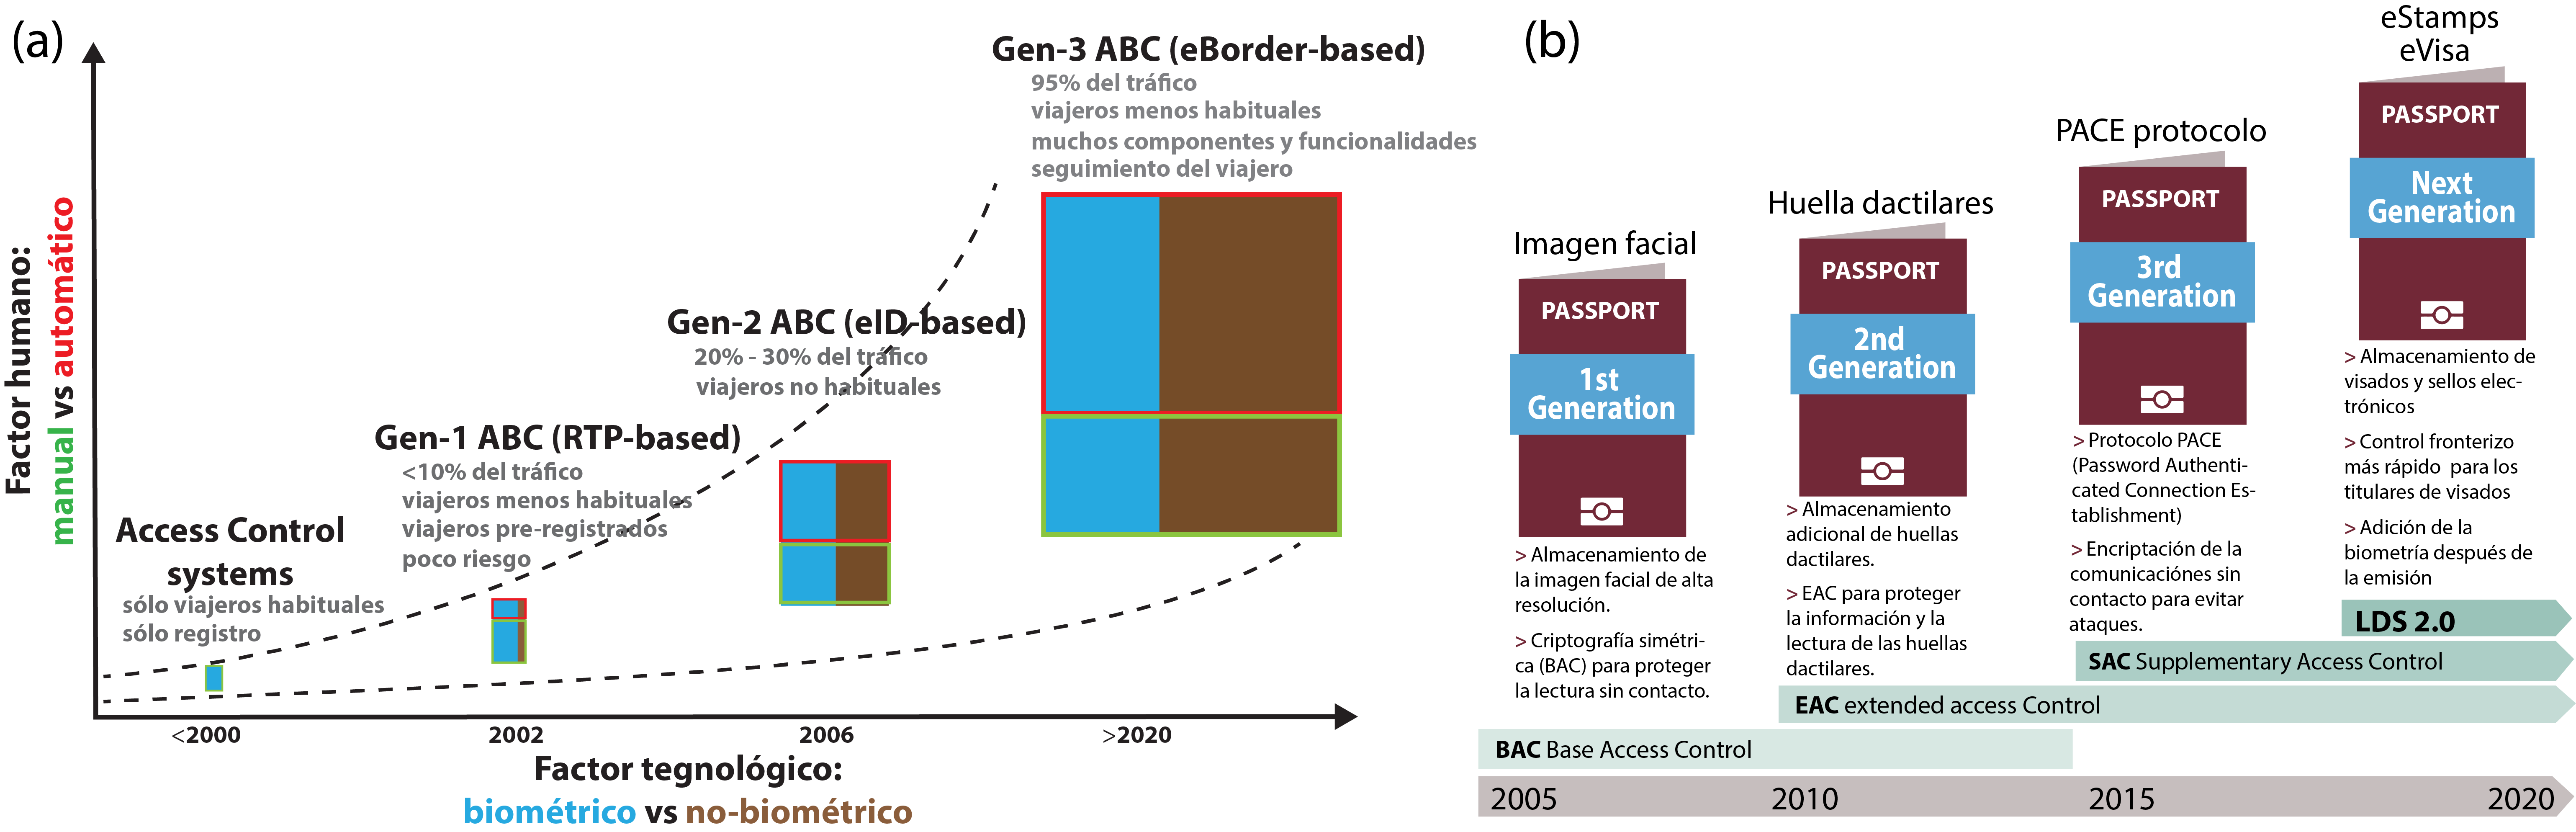
\includegraphics[width=\textwidth]{ch-sistemasABC/images/ch-introduccion/GENEALOGIAS_DE_ABCS_Y_PASAPORTES.png}
     \caption{(a) Evolución de los sistemas \GLS{ABC} y (b) Generaciones para documentos de viaje fijado por \GLS{ICAO}\cite{ICAOOnline}.}
     \label{fig:generacionesABC_Pasaportes}
\end{figure}

A finales del siglo XX se empezaron a buscar formas de automatizar los cruces fronteras. Por ejemplo, en el aeropuerto \textit{Schiphol} de Amsterdam, en $1992$, se empezaron a tomar las huellas dactilares de viajeros frecuentes. Y en $1998$, Malasia, fue el primer país del mundo en emitir pasaportes electrónicos. Pero no fue hasta $2004$, cuando Bélgica lanza el primer pasaporte electrónico adaptado al estándar que un año antes había presentado la \textit{International Civil Aviation Organization} (\gls{ICAO} \cite{ICAOOnline}) para los \textit{Machine Readable Travel Documents} (\gls{MRTD} \cite{doc20069303}). Este estándar es considerado la primera generación de documentos de viaje electrónicos e incluían un circuito integrado con los datos de identificación y la fotografía del titular. A partir de ese momento \GLS{ICAO} ha ido introduciendo mejoras que incrementan las medidas de seguridad. En Fig. \ref{fig:generacionesABC_Pasaportes} (b) se puede ver la evolución de las distintas generaciones de pasaportes electrónicos propuestas por la \GLS{ICAO}.

\medskip
\textbf{Sistemas \GLS{ABC}} 
\medskip

% color{cyan}SECRIP
% En un informe anual publicado por la compañía \textit{Boeing} \cite{BoeingOnline}, la previsión del crecimiento del tráfico de viajeros de aeronaves en todo el mundo alcanza una cantidad de casi el $5$\% en el período $2015$-$2035$ (\cite{Boeing2016}). Este aumento se espera que se duplique hasta el $9,5$\% para el área específica de Asia meridional en el mismo período. Estos números sugieren que se necesita hacer un gran esfuerzo en los próximos años en los controles de seguridad en los puntos de control de fronteras aéreas. Otros tipos de fronteras, como las de
% puertos marítimos y fronteras terrestres, también se espera que sufran de un importante aumento del tráfico \cite{donida2016emerging}.


% Cada día se cruzan millones de fronteras en todo el mundo. Se estima que alrededor de $3,5$ millones de personas cruzaron las fronteras internas entre los países de \textit{\Gls{Schengen}} diariamente en $2017$ \cite{migration2018report}. En el caso de los Estados Unidos, el número de cruces fronterizos en el mismo año fue de aproximadamente $400$ millones \cite{cbp2018snapshot}, mientras que en el Reino Unido se alcanzó la cantidad de $314$ millones \cite{ukborder2017audit} en $2016$.
% \color{black}

% En todos estos cruces fronterizos, los agentes de seguridad tienen que discernir lo antes posible: quién puede o no entrar en el país según las políticas de inmigración o los aspectos de seguridad nacional, si un viajero figura en una lista de sospechosos, actualizar las bases de datos correspondientes o incluso, en algunos casos, sellar el pasaporte del viajero. En conjunto, todas estas operaciones se convierten en una tarea que consume mucho tiempo. De este modo, es necesario dotar a los funcionarios de aduanas y fronteras con procedimientos e instrumentos rápidos y eficaces para garantizar un cómodo cruce de frontera sin colas para los viajero, mientras se mantiene el control del flujo de viajeros. 

Los agentes de frontera deben decidir quién puede pasar al país. Para ello deben tener en cuenta: aspectos de seguridad nacional, políticas de inmigración o si el viajero figura en alguna lista de sospechosos. Además tienen que consultar y actualizar las bases de datos correspondientes y en algunos casos hasta sellar los documentos de viaje. Todas estas tareas consumen mucho tiempo por lo que es necesario dotar a los funcionarios de aduanas y fronteras con procedimientos e instrumentos eficaces para agilizar el tránsito de viajeros. 

En paralelo a la evolución de los documentos de viaje han evolucionado también, los procedimientos y las tecnologías empleadas en los cruces de frontera. Las primeras puertas con lectura de pasaportes se instalaron en Reino Unido, Desde $2008$, y desde entonces los sistemas han ido evolucionando. En los últimos años han surgido los llamados sistemas \textit{Automated Border Control} (\GLS{ABC}). Sistemas automáticos que realizan tres operaciones fundamentales: (1) Autenticación automática de la documentación del viajero, (2) verificación de la identidad de el viajero como titular legítimo de la documentación, mediante procesos biométricos, y (3) Comprobación del permiso para cruzar la frontera atendiendo a las reglas predefinidas. En la figura \ref{fig:generacionesABC_Pasaportes} (a), se observa la evolución de estos sistemas, incrementado la automatización (rojo) frente a los proceso manuales (verde) y también han pasado de ser herramientas de apoyo para los agentes, en la verificación biométrica (azul) a incluir otros procesos, no exclusivamente biométricos (marrón). 

% Todo esto se hace con mínima o ninguna intervención humana \cite{FRONTEX2012OpeReport}.

% (\GLS{ABC}) \cite{del2016automated} para ayudar a las autoridades fronterizas automatizando (totalmente o al menos parcialmente) el proceso. Así, los sistemas \GLS{ABC} se han extendido a todo tipo de fronteras. Los sistemas \GLS{ABC} reducen las habituales molestias de los controles fronterizos y aumentan la satisfacción de los viajeros. Las lineas aéreas y los aeropuertos optimizan sus recursos y los agentes de seguridad pueden centrar su trabajo en las alertas importantes.

% Estos sistemas aumentan el flujo de viajeros a través de la frontera mientras mantienen el control sobre los temas de seguridad. Se basan en documentos de viaje legibles por máquina, como pasaportes, visados, tarjetas de identidad o incluso tarjetas de viajero frecuente. Estos documentos contienen un chip con información como los datos personales del viajero y algunos rasgos biométricos (por ejemplo, el rostro, las huellas dactilares y el iris).


\medskip
\textbf{Sistemas ABC en Europa} 
\medskip

Los sistemas \GLS{ABC} en la Unión Europea (\GLS{EU}) tienen unas características muy especificas. Con la creación del área \Gls{Schengen} en $1995$, se aprobó una nueva política de fronteras para los estados miembros donde sólo se mantuvieron las fronteras exteriores, es decir, con los países fuera del área\footnote{Actualmente, $26$ países europeos pertenecen al área \Gls{Schengen}, de los cuales $4$ no son miembros de la Unión Europea (\GLS{EU}) (Noruega, Islandia, Suiza y Liechtenstein). En un futuro próximo, cuatro miembros más (Bulgaria, Croacia, Chipre y Rumania), estarán obligados a unirse, mientras que los Estados Unidos, Reino Unido e Irlanda han optado por quedarse fuera. También, tres microestados europeos, como Mónaco, San Marino y Ciudad del Vaticano, son miembros de facto. Toda el área \Gls{Schengen} comprende una superficie superior a $4,3$ millones de metros cuadrados y una población de casi $420$ millones de personas,}. Todas las normativas, protocolos y procedimientos para las fronteras en el área \Gls{Schengen} están definidos en \textit{Schengen Borders Code} (\GLS{SBC}) \cite{SBCode2016}. Los viajeros de un estado miembro pueden pasar a otro sin controles fronterizos. Mientras que los viajeros de los estados no miembros, o viajeros de terceros países (\GLS{TCN}), están obligados a cruzar un control fronterizo. Estos Los viajeros pueden encontrarse en dos situaciones legales: los viajeros sin necesidad de un visado (\textit{Third Country Nationals Visa-exempt} (\GLS{TCNVE})), o los que necesitan \gls{visa} o un permiso de residencia (\textit{Third Country Nationals Visa Holders} (\GLS{TCNVH})). Para cada uno de estos tipos de viajeros hay un procedimiento diferente definido en el \GLS{SBC}.

En $2004$ fue fundada la \textit{European Border and Coast Guard Agency} (\Gls{frontex} \cite{FRONTEXOnLine}) con el objetivo de mejorar la gestión de las fronteras exteriores de los estado miembros. 

\medskip
\textbf{Proyecto ABC4EU} 
\medskip
 
Gran parte de los trabajos realizados y las invitaciones presentadas en este documento forma parte de la labor de colaboración llevadas a cabo en el proyecto \GLS{ABC4EU}, 2014 \cite{ABC4EUOnline}. Este proyecto, dentro del Séptimo Programa Marco de la \gls{EU} (\GLS{FP7}), tenia como objetivos mejorar el flujo de trabajo y las funcionalidades de los \GLS{ABC} para todo tipo de fronteras (aeropuertos, puertos y fronteras terrestres) en la \GLS{EU}. Identificar problemas y definir los requisitos de estos sistemas dentro del área \Gls{Schengen}. Varias instituciones de ocho países europeos (Estonia, Finlandia, Alemania, Irlanda, Italia, Portugal, Rumanía, y España) formaron parte del proyecto.

El principal objetivo del proyecto es el diseño de un sistema \GLS{ABC}, cuya prioridad fuera la seguridad, para viajeros \GLS{TCN}, tanto \GLS{TCNVE} como \GLS{TCNVH}. El sistema propuesto debía conformarse a las reglas definidas en \GLS{SBC} ya que manejaba dos importantes bases de datos información sensible \footnote{El proyecto \GLS{ABC4EU} tiene en cuenta la normativa sobre el tratamiento de datos personales de las personas físicas establecido por la \GLS{EU} y por cada país en particular, definido en la directiva $95$/$46$/CE del paramento europeo y del consejo \cite{europea1995directiva}.}: Sistema de Información de Visados (\GLS{VIS}), con información biométrica, y el  \Gls{Schengen} Sistema de Información (\GLS{SIS}) con información sobre actividades delictivas.

\medskip
\textbf{Futuros \Gls{ABC}} 
\medskip

La tendencia indica que los sistemas \GLS{ABC} es separar el proceso en dos etapas: registro y validación. El registro y la validación podrán estar separados para que de esta manera el viajero pueda registrarse de marea previa al viaje.

Los dispositivos \GLS{ABC} en los cruces de frontera tendrán una captura dinámica (\Gls{OnTheFly}) de forma que los viajeros no tengan que detenerse y así agilizar el flujo de viajeros.

\medskip
\textbf{Ataques de presentación} 
\medskip

% El proceso de reconocimiento facial es un reto de identificación biométrica bien conocido debido a las altas tasas de precisión alcanzadas y a la baja intrusión en los sujetos identificados.
% Para abordar el proceso de autenticación facial, hay varios métodos. Algunos de estos enfoques tienen requisitos de seguridad elevados. Un ejemplo es el sistema de control fronterizo automático (\GLS{ABC}), en el que se utiliza el rasgo biométrico para controlar y garantizar el proceso de cruce de fronteras. El proceso de autenticación del \GLS{ABC} tiene que determinar si existe o no coincidencia entre la imagen facial almacenada en el(\GLS{eMRTD}) y una captura \textit{in situ}.

% Los sistemas ABC están expuestos a múltiples ataques o amenazas, por ejemplo, robo de identidad o fraude, lo que también se llama "\textit{\gls{spoofing}}". Por esta razón, muchos trabajos de investigación actuales centran su atención en las técnicas \textit{\gls{antispoofing}} \cite{del2017face}.

% En los últimos años, el amplio uso de los sistemas \GLS{ABC} en los aeropuertos ha aumentado la atención y el estudio de las posibles amenazas múltiples (por ejemplo, el ataque a la presentación) como explica la \textit{European Border and Coast Guard Agency} (\GLS{frontex}) \cite{FRONTEXOnLine}, \cite{FRONTEX2016TechReport}. Estos ataques incentivan la proliferación de algoritmos sobre detección de ataques de presentación (\GLS{PAD}) \cite{jia2019survey}, \cite{ramachandra2017presentation}, \cite{damer2016practical} 

% Millones de pasajeros viajan cada día, siendo el cruce de fronteras una de sus actividades más comunes. En estos puntos es extremadamente importante que la seguridad esté completamente garantizada. Sin embargo, el mantenimiento de niveles de seguridad adecuados es una cuestión muy exigente. Esto ha promovido el desarrollo de sistemas capaces de proporcionar apoyo a las autoridades fronterizas mediante la automatización de algunas de sus tareas. 

Los sistemas \GLS{ABC} se han convertido en una herramienta clave en los cruces de fronteras. Aumentan el flujo de viajeros ya que pueden lograr evaluaciones rápidas de las personas a través de la verificación biométrica de sus documentos \gls{eMRTD}. Sin embargo, esto ha motivado que la aparición de ataques a este tipo de sistemas se haya incrementado notablemente. Los ataques más comunes son los ataques de presentación (\textit{presentation attack} \GLS{PA}) que consisten en la suplantación de la identidad del viajero (\gls{spoofing}). Son relativamente fáciles de llevar a cabo y no requieren un gran conocimiento de la implementación interna del sistema. Paa hacer frente a este tipo de amenazas los \GLS{ABC} se han dotado de métodos \gls{antispoofing} o \textit{Presentation Attack Detection} (\GLS{PAD}).

% Una de las tareas que realizan los sistemas \GLS{ABC} es la identificación biométrica del viajero. Esto se realiza gene ralmente comparando el rostro capturado del sujeto en posición frontal estática con la imagen del rostro almacenada en el pasaporte. Para esta configuración (el sujeto se sitúa delante de la cámara), los sistemas han incluido diferentes algoritmos de Detección de Ataque de Presentación (\GLS{PAD}) (véase, por ejemplo, \cite{ramachandra2017presentation}). Esto ha aumentado su capacidad de detectar diversos tipos de ataques como máscaras, fotos impresas o vídeos en pantalla. En cualquier caso, la mayor parte de la responsabilidad de la detección de ataques recae en los guardias fronterizos que supervisan el sistema.

\medskip
\textbf{Ataques \Gls{morphing}} 
\medskip

El \gls{morphing} es uno de los \GLS{PA} más peligrosos ya que los sistemas biométricos no suelen ser capaces de detectarlos. El \gls{morphing} consiste en fusionar dos imágenes para obtener una imagen intermedia. El proceso de morphing surgió en el mundo de las artes visuales y los efectos especiales, pero al alcanzar tan alto grado de precisión, rápidamente se convirtió en una amenaza para los sistemas biométricos. Cómo \GLS{PA}, en \gls{morphing} consiste en generar una imagen qué combina los rasgos biométricos de varios individuos. Aunque es posible realizar este proceso con distintos rasgos biométricos (iris, huellas dactilares), habitualmente, el \gls{morphing}, se realiza con caras. En los sistemas \gls{ABC}, el ataque de morphing consiste en reemplazar la imagen almacenada en los \gls{eMRTD} de un viajero genuino y reemplazarla por una imagen que mezcla los rasgos genuinos con los de otro individuo impostor, qué tratará de cruzar la frontera con los documentos manipulados.

En los últimos años se han incrementado las investigaciones sobre métodos \GLS{PAD} para detectar ataques \gls{morphing}, estos métodos 
se conocen como métodos \textit{Morphing Attack Detection} (\GLS{MAD}).

% El proceso de \gls{morphing} surgió en el mundo de las artes visuales en películas, vídeos musicales o anuncios, para lograr efectos especiales sorprendentes \cite{lee1998polymorph,ucicr1992feature}. En un principio, el proceso se realizaba manualmente pero rápidamente aparecieron los primeros algoritmos que automatizaron las tareas de \gls{morphing} \cite{wolberg1998image}. Incluso para los expertos resultaba difícil distinguir si una imagen ha sido manipulada mediante \gls{morphing} \cite{beale1995categorical}, \cite{levin2000categorical}, \cite{robertson2018detecting}. Así, la técnica evolucionó de recurso artístico a ser una herramienta delictiva \cite{ferrara2014magic}.

% El \gls{morphing} como ataque de presentación en los sistemas biométricos consiste en generar una imagen mezclando los rasgos de dos sujetos diferentes (el \gls{genuino} y el \gls{impostor}). Comúnmente el \gls{morphing} se realiza con imágenes faciales pero también es posible el \gls{morphing} de otros rasgos biométricos, como el iris \cite{rathgeb2017feasibility} o la huella dactilar \cite{ferrara2016feasibility}.

% En el caso de los sistemas \GLS{ABC} el ataque de \gls{morphing} consiste en manipular la imagen de la cara almacenada en el \textit{chip} del \gls{eMRTD} y reemplazándola por otra que fusiona la identidad del propietario real del documento (que puede o no se cómplice del atacante) y la del viajero \gls{impostor}. En el cruce de fronteras se realiza la comparación de la imagen capturada en el \GLS{ABC} (\textit{vivo}) y la imagen almacenada en el \gls{eMRTD}, entonces, el sistema debe distinguir si el viajero es quien dice ser. La respuesta habitual de esta verificación es la aceptación, teniendo en cuenta la gran similitud entre el rostro del viajero \gls{impostor} y el \gls{morphing} del \gls{eMRTD}.

% Puede considerarse como una de las amenazas más importantes para los sistemas \GLS{ABC} \cite{ramachandra2019towards}, \cite{ferrara2018face}, \cite{makrushin2018overview}, \cite{scherhag2017vulnerability}, \cite{scherhag2020deep}. Se requieren módulos \textit{Morphing Attack Detection} (\GLS{MAD} \cite{scherhag2017vulnerability}, \cite{scherhag2019face}) específicos para la detección de este tipo de ataques presentación.

% En los últimos años se han incrementado las investigaciones sobre \GLS{MAD} e incluso se ha organizado la primera competición \textit{Face Recognition Vendor Test MORPH} del \textit{National Institute of Standards and Technology} (\GLS{NIST}) \cite{frvtMorphOnLine} para tener una visión global y un \textit{ranking} del rendimiento de los algoritmos \GLS{MAD} actuales.


%%%%%%%%%%% OBJETIVOS   %%%%%
\section{Objetivos\label{sec:objetivos}}
% En primer lugar, aborda los sistemas \GLS{ABC} detallando sus configuraciones, diseños posibles y despliegue en entornos reales. A continuación se presentan los ataques de presentación, estableciendo una clasificación básica y describiendo los instrumentos más típicos utilizados para lograrlos. Finalmente, se presentan los sistemas \GLS{PAD}, ilustrando su funcionamiento, evaluando las tecnologías consideradas y sus puntos fuertes y débiles.

Estudiar el estado del arte de los sistemas \GLS{ABC} en general y especialmente en el contexto de la zona \Gls{Schengen}.

Estudiar el estado del arte de los ataques de presentación sistemas biométricos.

Analizar la problemática de los ataques de presentación en los sistemas \GLS{ABC}.

Participar en la puesta en marcha de un sistema \GLS{ABC} en el entorno real de un cruce de fronteras.
 
Señalar los distintos tipos de sistemas \GLS{ABC}.

Estudiar cómo se organiza es un sistema biométrico dentro de los sistemas \GLS{ABC}.
  
Estudiar los puntos débiles del módulo de captura del subsistema biométrico de los sistemas \GLS{ABC}.


Poner a prueba algunos de los algoritmos con mejor rendimiento

Poner a prueba el rendimiento, en un entorno real, DE los algoritmos PAD mejor valorados en la literatura.

Proponer un método de PAD para la ataques de presentación con morphing.

Analizar y evaluar sistema biométrico de verificación facial de un sistema \GLS{ABC} segregado en dos pasos.

Proponer una arquitectura para un módulo de \GLS{PAD} en un sistema \GLS{ABC} captura dinámica.



%%%%% ESTRUCTURA DE LA TESIS %%%%%
\section{Estructura del documentos\label{ch:estructura}}

Este documento se divide en 9 capítulos.

Este primer capítulo presenta una introducción el tema de los sistemas \GLS{ABC} y a la amenaza qué suponen los ataques de presentación para estos sistemas. Además, se detallan los objetivos que busca el presente estudio.

El Capítulo \ref{ch:EstadoDelArte} es una recopilación de un gran número de investigaciones que abordan los temas a tratar en este estudio. Este estado del arte está organizado entre secciones, enfocadas cada una de ellas a un aspecto de la tesis: Sección \ref{sec:estadoArteABC}, sobre sistemas \GLS{ABC}, Sección \ref{sec:estadoArteAtaquesPresentacion}, sobre ataques de presentación y Sección \ref{sec:estadoArteMorphing} centrada en ataques de presentación con \gls{morphing}.

El Capítulo \ref{ch:introSistemasABC} presenta una contextualización de los sistemas \GLS{ABC} en la Sección \ref{sec:sistemasABC} y de los ataques de presentación en la Sección \ref{sec:ContextoAtaquesPresentacion}.

El capítulo \ref{ch:BBDDs} describe cada una de las bases de datos construidas para llevar a cabo los experimentos y las investigaciones realizadas.

El capítulo \ref{ch:PAD_MULTIATAQUE} pone a prueba de alguno de los algoritmos del estado del arte con mejores rendimientos, usando datos capturados por sistema \GLS{ABC} en un entorno real. Y propone un método \GLS{PAD} para hacer frente a diferentes tipos de ataque.

El capítulo \ref{ch:EVALUACIONACION_TOPOLOGIAS} analiza el subsistema biométrico de un sistema \GLS{ABC} de dos etapas segregadas. Además de evaluar la doble verificación características de estos sistemas. Se propone un \GLS{PAD} y se evalúa su rendimiento en ambas capturas.

El capítulo \ref{ch:morphing} expone la problemática de los ataques de presentación con \gls{morphing} y propone un método de \GLS{PAD} para la detección de este tipo de ataques.

El Capítulo \ref{ch:ABC_OnTheFly} expone la problemática de los ataques de presentación en sistemas \GLS{ABC} con captura dinámica (\Gls{OnTheFly}). Y propone una arquitectura para un módulo \GLS{PAD} que sea adapta a este tipo de sistemas.

El capítulo \ref{ch:conclusion} presenta las conclusiones extraídas con cada una de las investigaciones presentadas en los capítulos anteriores y las contribuciones que cada una de ellas aposta.


%%%%%%%%%%% ESTADO DEL ARTE    %%%%%%%%%%
\chapter{Estado del Arte\label{ch:EstadoDelArte}}

En este Capítulo se presenta el estado del arte de los sistemas \Gls{ABC} en la Sección \ref{sec:estadoArteABC}. En la sección \ref{sec:estadoArteAtaquesPresentacion} de los ataques de presentación y específicamente, de los ataques de presentación con \gls{morphing} en la sección \ref{sec:estadoArteMorphing}.

%%%%%%% ESTADO DEL ARTE DE LOS SISTEMAS ABC %%%%%%%%%%%%
\section{Sistemas ABC}\label{sec:estadoArteABC}

Los \GLS{ABC} son sistemas multi-sensor con tres tareas principales: Primero, digitalizar la documentación del viajero y autentificar su validez. Después, comprobar que el viajero es quien dice ser, mediante una verificación biométrica entre los rasgos del viajero y los almacenados en los documentos (comúnmente rasgos faciales y dactilares). Y finamente, comprobar si el viajero tiene derecho a cruzar la frontera. según las normas administrativas y legales. Algunos sistemas \cite{didier2015eu} \cite{anand2016enhancing} \cite{del2016automated} \cite{Gorodnichy2015ARTinABC} separan en estas tareas en dos etapas: Una etapa de registro (\GLS{RTP}, \textit{Register Traveller Programme}) y otra de validación (\GLS{EES}, \textit{Entry/Exit System}). En el registro, se auténtica documentación y se comprueba la idoneidad para cruzar la frontera, mientras que la verificación biométrica, se realiza en la validación. En ocasiones. estás dos etapas lógicas se separan físicamente en dos dispositivos, dando lugar a una topología de \GLS{ABC} segregada \cite{del2016automated}.

\begin{figure}[t]
    \centering
    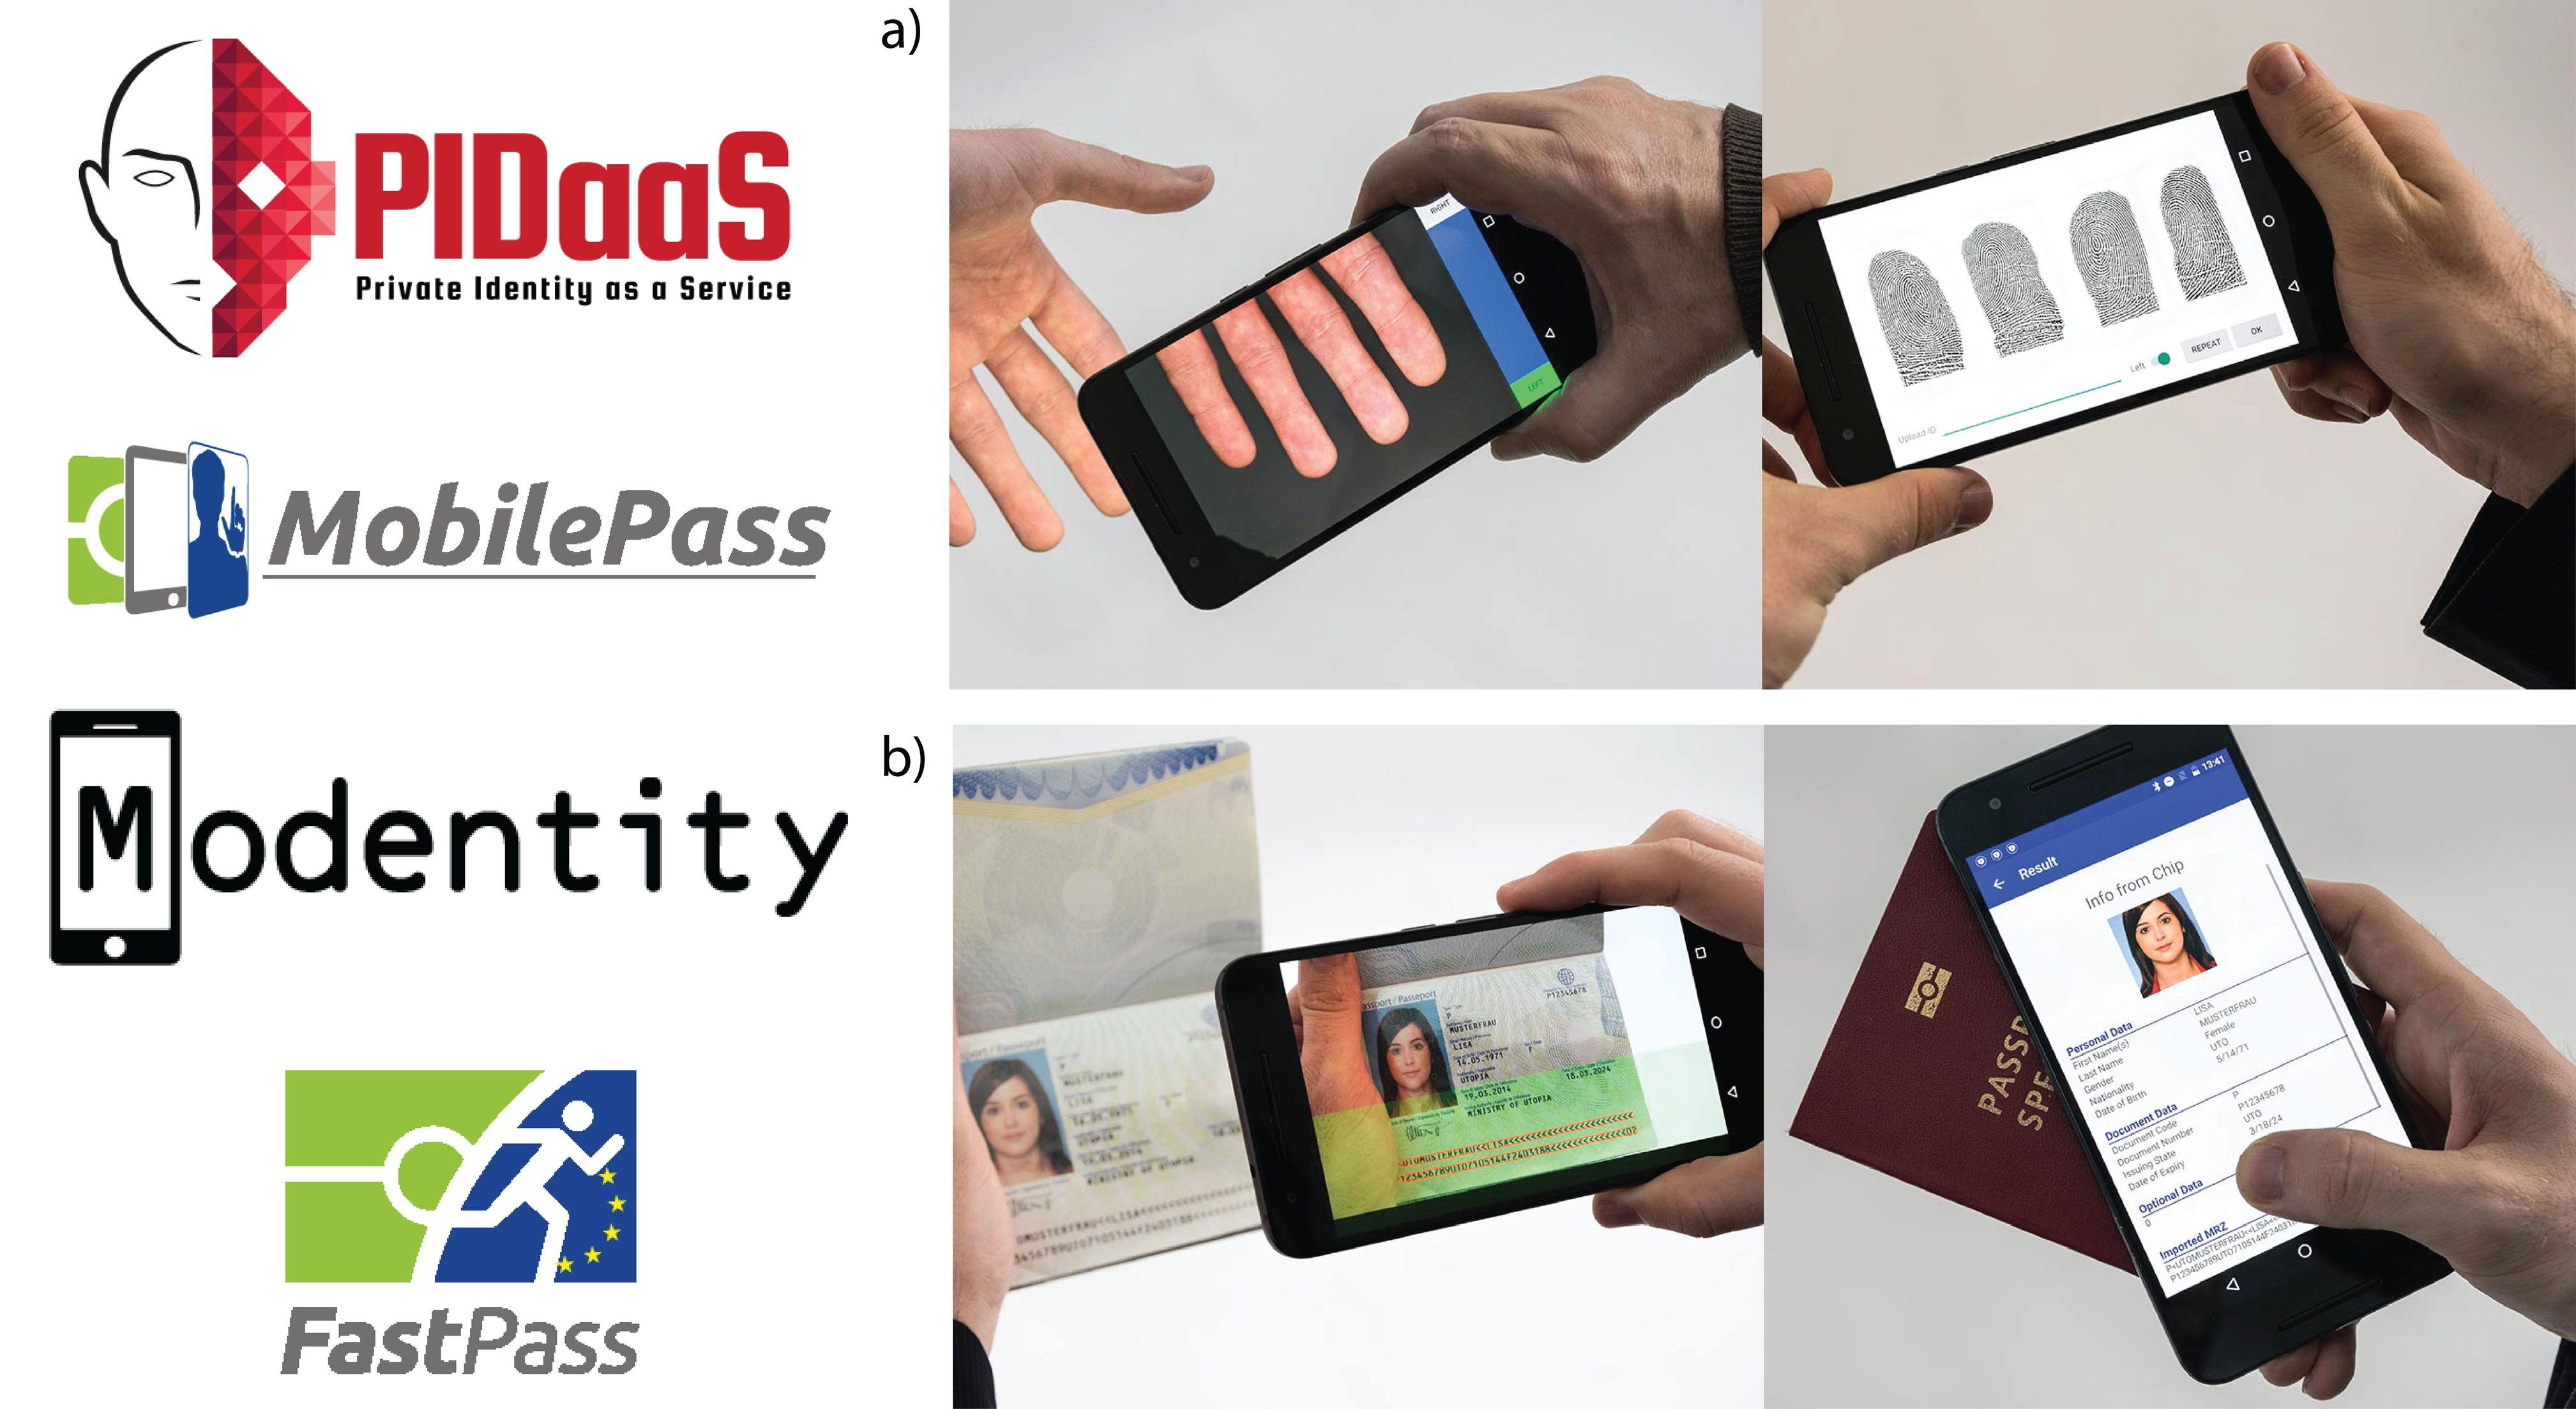
\includegraphics[width=0.9\textwidth]{ch-sistemasABC/images/ch-SistemasABC/CAPTURA_MOBIL_Y_PROYECTOS.png}
    \caption{A la izquierda Proyectos de investigación y empresas dedicados a sistemas móviles: \Gls{MobilePass}\cite{MobilePassOnline}, \Gls{Modentity}\cite{ModentityOnline}, \Gls{PIDaaS}\cite{PIDaaSOnline}. Y a la derecha, funcionalidades de los sistemas \GLS{ABC} móviles del proyecto \gls{Modentity} \cite{ModentityOnline}. a) Verificación dactilar sin contacto y b) Digitalizado y lectura \GLS{NFC} de un pasaporte}
    \label{fig:modentityFunciones}
\end{figure}

\begin{figure}[t]
    \centering
    
\includegraphics[width=0.8\textwidth]{ch-sistemasABC/images/ch-SistemasABC/LOGOS_EMPRESAS.png}
    \caption{Empresas dedicadas a sistemas \GLS{ABC}:\Gls{MODI} \cite{MODIOnline}, \Gls{INDRA} \cite{indraOnline}, \Gls{VisionBox} \cite{visionBoxOnline}, \Gls{Gemalto} \cite{gemaltoOnline}, \Gls{ARH} \cite{ARHOnline},\Gls{Innovative} \cite{InnovativeOnline}}
    \label{fig:logosEmpresasABC}
\end{figure}

Para su homologación, los sistemas \GLS{ABC}, deben ajustarse a la legislación de fronteras de cada país, por ejemplo al \GLS{SBC} \cite{SBCode2016} en \GLS{EU}. Y también, satisfacer ciertos estándares internacionales cómo los fijados para sistemas biométricos de \GLS{ISO}/\GLS{IEC} $19794$ \cite{ISO/Biometric} o los de uso de documentos \gls{eMRTD} de \GLS{ICAO} Doc $9303$ \cite{doc20069303}. Del mismo modo es conveniente que tengan en cuenta las recomendaciones técnicas \cite{FRONTEX2016TechReport} y operativas \cite{FRONTEX2016OpeReport}, presentadas por \Gls{frontex} \cite{FRONTEXOnLine}. 

El subsistemas biométrico es un componente fundamental en los \GLS{ABC} \cite{labati2016biometric} \cite{spreeuwers2012evaluation}. Es posible encontrar sistemas que hacen uso de diferente rasgos biométricos: huellas dactilares \cite{anand2016enhancing} \cite{gamassi2005robust}, la cara \cite{del2015face} \cite{del2016automated} \cite{kosmerlj2006face}, el iris \cite{daugman2015iris} \cite{palmer2012ten} \cite{matey2006iris}, e incluso sistemas con biometría palmar (geometría de la mano) \cite{nanavati2011biometric}. Pero la tendencia es usar sistemas multi-biométricos \cite{cantarero2013multi} \cite{cimato2006personal} \cite{cimato2008privacy} \cite{gamassi2004high} \cite{gamassi2005multi}.

% %BIOMETRIA DEL IRIS EN LOS SISTEMAS DE ABC DE CRUCE DE FRONTERAS
% @article{daugman2015iris,

% %PRESENTA LOS PROBLEMAS DE LA BIOMETREIA DEL IRIS EN LOS SITEMAS ABC
% palmer2012ten,

% %RECOCIMIENTO DEL IRIS EN MOVIMIENTO 
% matey2006iris

Los sistemas \GLS{ABC} están en continua evolución, asimilando tecnologías emergentes y nuevos desarrollos. Muchas instituciones gubernamentales, nacionales e internacionales, gestionan proyectos de investigación dedicados este tipo de sistemas, como: \GLS{ABC4EU} \cite{ABC4EUOnline}, \Gls{FastPass} \cite{FastPassOnline}, \cite{berglund2008frontex} o \cite{kosmerlj2006face}. También en el sector privado, muchas empresas se dedican a la investigación y al desarrollo de este tipo de sistemas: \Gls{MODI} \cite{MODIOnline}, \Gls{INDRA} \cite{indraOnline}, \Gls{VisionBox} \cite{visionBoxOnline}, \Gls{Gemalto} \cite{gemaltoOnline}, \Gls{ARH} \cite{ARHOnline}, \Gls{Innovative} \cite{InnovativeOnline}. Y otras como: \Gls{Cognitec} \cite{cognitec2019url} o \Gls{Dermalog} \cite{DermalogOnline} proporcionan desarrollos cruciales para el subsistemas biométricos de los \GLS{ABC}.     

% En el caso de los cruces de frontera europeos en los que se utilizan sistemas \GLS{ABC}, se requiere comprobar la identificación del sujeto con dos listas: \GLS{RTP} (\textit{Register Traveller Programme}) y \GLS{EES} (\textit{Entry/Exit System}) \cite{didier2015eu}. La identidad de los viajeros y su idoneidad para cruzar la frontera se verifica en el control del \GLS{RTP} según la información almacenada en su documentación. Una vez identificados los viajeros, se registran sus datos. En el momento de cruzar la frontera, el \GLS{EES} obtiene la coincidencia biométrica entre la información registrada y los datos capturados.

% Dependiendo de los dispositivos en los que se realizan los procesos de \GLS{RTP} y \GLS{EES}, hay diferentes topologías de sistemas \GLS{ABC}: Proceso de un paso y proceso de dos pasos \cite{anand2016enhancing}. En la topología del proceso de un solo paso, la \GLS{RTP} y el \GLS{EES} se fusionan en un solo proceso en el que la identificación de los viajeros se lleva a cabo al mismo tiempo que éstos cruzan la frontera. Los dispositivos para este tipo de topología suelen ser trampas electrónicas \cite{del2016automated}, que no permiten el cruce hasta que la identificación se haya realizado correctamente. En la topología de proceso en dos etapas, los procesos \GLS{RTP} y \gls{EES} están bien diferenciados. Primero, se registran los viajeros y luego, su información biométrica se compara antes de permitir el cruce. Se puede considerar que el \GLS{ABC} de dos pasos integrado o segregado atiende si el\GLS{RTP} y el \GLS{EES} se logran a través de uno o dos dispositivos. 

% En cuanto a la implantación de los sistemas \GLS{ABC} y su utilidad, es importante mencionar que casi todos los aeropuertos que reciben viajeros de países no pertenecientes a \Gls{Schengen} los utilizan (un mapa completo de los aeropuertos con \GLS{ABC} se presenta en \cite{iata2018abc}). Sin embargo, los puertos marítimos equipados con \GLS{ABC} no son tan comunes. 

% Los sistemas \GLS{ABC} pueden tener varias configuraciones físicas \cite{morosan2018information}. Las más típicas utilizan puertas electrónicas (\gls{e-gate}) \cite{donida2016emerging}. Estos dispositivos regulan el flujo de viajeros a través de la frontera mediante el uso de sensores biométricos (por ejemplo, cámaras de reconocimiento facial \cite{labati2016biometric} y lectores de huellas dactilares \cite{anand2016enhancing}, lectores de documentos de viaje (por ejemplo, escáneres \cite{nguon2017system} y lectores de chip sin contacto por radiofrecuencia \cite{abdal2016authentication}, así como barreras físicas que permiten (o no) al viajero cruzar la puerta electrónica \cite{nieto2014walls}.

% Profundizar en el diseño de los sistemas \GLS{ABC}, su capacidad para volver a cubrirse de situaciones problemáticas (es decir, la resistencia) y para resistir ataques externos (es decir, la robustez) son sus principales requisitos de seguridad. La mayoría de los ataques típicos se centran en el sistema biométrico. Estos ataques se denominan ataques de presentación, que consisten en que un atacante presenta características biométricas falsificadas de otro sujeto a los sensores para obtener permiso para cruzar la frontera. Por esta razón, los sistemas \GLS{ABC} incluyen algún tipo de \GLS{PAD} y módulo \GLS{PAD} en el proceso de reconocimiento biométrico. 

% Los sistemas \GLS{ABC} hacen uso de puertas electrónicas (\gls{e-gate}), que son dispositivos para controlar de forma automática el flujo de viajeros que cruzan la frontera por medio de elementos móviles o fijos, escáneres para la lectura de documentos y sensores para realizar captura biométrica. En particular, el viajero  presenta su \gls{eMRTD} al escáner del sistema, que detecta y extrae sus datos personales de la llamada zona de lectura mecánica \GLS{MRZ} del documento (figura \color{red} Alguien en el registro, en el paper era una de Cristina\color{cyan}). Una consulta a la base de datos de cruces permitidos viajero se hace y luego, si se tiene éxito, el los datos biométricos del viajero se extraen del chip del documento. Estos datos pueden incluir un conjunto de fotos faciales, huellas dactilares, etc. El viajero entonces tiene que proveer al sistema \GLS{ABC} con su sistema biométrico características en ese mismo momento (\gls{vivo}), que se comparan con los que se leen en el chip del documento. Si es una coincidencia, entonces la puerta electrónica abre las puertas y se permite a los viajero cruzar la frontera.

% Existen tres configuraciones posibles para un sistema \GLS{ABC} (Ver Fig. \ref{fig:TopologiasABC}): Primero, un viajero a la vez se hace entrar en una trampa, que es un cubículo con dos puertas. En este espacio, tanto la autenticación del documento y la verificación biométrica se hacen en paralelo en un proceso de un solo paso, por lo que esta solución puede ser muy rápida. Las otras dos configuraciones utilizan un proceso de dos pasos. Por un lado, la solución integrada, en la que la autenticación de los documentos tiene lugar justo fuera de un Figura \color{red}ESTA ES LA IMAGEN DE CRISTINA EN EL REGISTRO DE BARAJAS\color{cyan}: Ejemplo de un \GLS{ABC}. Foto tomada del piloto experiencia en el Aeropuerto Adolfo Suárez Madrid-Barajas T$4$-$S$ terminal de llegadas internacionales \cite{aeropuertoMadridBarajas}, \gls{mantrap}, dentro de la cual se lleva a cabo la captura biométrica.

% En una tercera configuración, la solución segregada, la autenticación de documentos y la biométrica la verificación se realiza en un quiosco de inscripción, mientras que se hace una segunda verificación biométrica en la puerta única \gls{e-gate}.

% Para más información sobre el \GLS{ABC}, el lector puede revisar \cite{labati2016biometric}, que proporciona un estudio sobre el reconocimiento biométrico en los sistemas \GLS{ABC}, mientras que \cite{del2015face}, se centra específicamente en sistemas \GLS{ABC} basados en el reconocimiento facial.
% \color{black}

\color{red}
Ver cronología de publicaciones sobre los sistemas \GLS{ABC} (Apéndice \ref{apendix:ApendiceCronologiaABC})

Ver cronología de publicaciones sobre \gls{biometria} (Apéndice  \ref{apendix:ApendiceCronologiaBiometria})
\color{black}

%%%%%%% ESTADO DEL ARTE DE LOS ATAQUES DE PRESENTACION %%%%%%%%%%%%%%%%%%%%%%%%
\section{Ataques de presentación}\label{sec:estadoArteAtaquesPresentacion}

El sistemas biométrico de los \GLS{ABC} puede ser atacado en diferentes etapas\footnote{\GLS{ISO}/\GLS{IEC} $30137$-$1$:$2019$ -  Part 1: System design and specification \cite{ISO/Biometric}}: en el sensor, en la base de datos, en las comunicaciones, o el modulo de proceso, etc.. Los ataques de presentación tienen lugar en el dispositivo en la fase de captura del sistema \cite{ratha2001enhancing}.

Una primera clasificación\footnote{\GLS{ISO}/\GLS{IEC} $30107$-$1$:$2016$ Biometric presentation attack detection — Part 1: Framework  \cite{ISO/PADFramework}} de estos ataques incluye: los ataques con base documental que requieren de la manipulación de los documentos de viaje: falsificaciones \cite{tolosana2019presentation} o \gls{morphing}  \cite{scherhag2018towards}), y de base biométrica que se basan en la suplantación (\gls{spoofing}) de los rasgos biométricos del viajero por parte del atacante.

Cuando el viajero proporciona sus características biométricas voluntariamente e interactúa con el sistema de la manera esperada, la presentación  se considera una presentación \gls{bona-fide}. Pero, cuando una persona trata de interferir con el funcionamiento normal del sistema, se considera un \GLS{PA}. El rasgo u artefacto utilizado en el ataque se llama \textit{Presentation Attack Instrument} (\GLS{PAI}). Existen distintos tipos de \GLS{PAI} (\GLS{ISO}/\GLS{IEC}, $2016$b \cite{ISO/PADFramework}): Una fotografía (impresa en papel \cite{scherhag2017vulnerability} \cite{rigas2015eye} \cite{anjos2011counter} o reproducida en una pantalla \cite{li2016generalized}), una máscara de cartón \cite{del2017face}, de silicona \cite{bhattacharjee2018spoofing} \cite{manjani2017detecting} o impresa en $3$D \cite{agarwal2017face}, una huella sintética \cite{sousedik2014presentation}, una imagen de alta resolución de iris \cite{raja2016color} o incluso el verdadero dedo de un cadáver \cite{deadFinger}.

Los \GLS{PAD} son métodos para la detección ataques de presentación \cite{marcel2014handbook}. Pueden ser métodos hardware o software.
Los métodos hardware se apoyan en el sensor y se basan en propiedades intrínsecas, como el pulso o el parpadeo de los individuos \cite{rigas2015eye}. En algunos casos el sistema produce un estímulo y espera una respuesta del viajero {\gls{challenge response}} \cite{shoukry2015pycra}.
Entre los métodos \textit{software} existen distintos enfoques en la literatura: Basados en micro-texturas, basados en la deformación de  los rasgos biométricos, basado en la búsqueda de artefactos, basado en la imagen espectral y enfoques híbridos.
Algunos de estos enfoques se basan en características temporales por lo que necesitan una captura de vídeo. 


% \cite{ramachandra2017presentation}. Los métodos basados en hardware (o a nivel de sensor) se basan en las propiedades intrínsecas del cuerpo. Nótese que, en algunos casos, se necesita un sensor específico o no convencional para adquirir estas características. Ejemplos de estas propiedades son: texturas faciales, resistencia eléctrica, temperatura, sudor, color, resistencia de la piel a otras longitudes de onda no visibles y forma tridimensional. Algunas de estas propiedades son involuntarias, ya que están controladas por el sistema nervioso, en particular el pulso, las sacadas oculares y la respiración. En el caso de los sistemas \GLS{PAD}, producen un estímulo y tratan de detectar las reacciones del cuerpo (métodos de desafío-respuesta) \cite{shoukry2015pycra}. Un ejemplo común de estos métodos es pedir al usuario que siga una luz con la cabeza, o que lea en voz alta una frase. Se pueden buscar reacciones involuntarias como el parpadeo de los ojos o la constricción de la pupila debido a la luz deslumbrante \cite{rigas2015eye}. Aunque estas tareas se pueden realizar por medio de software, también se pueden realizar por medio de hardware dedicado. Por último, el uso de estrategias multi-modales (mismo rasgo, múltiples sensores) o multi-biométricas (múltiples rasgos, mismo sensor) puede aumentar la robustez del sistema contra los ataques de suplantación de identidad

% Por el contrario, los métodos basados en software (o basados en rasgos) son capturados por un módulo situado justo después del sensor, funcionando así con la muestra biométrica adquirida. Esto proporciona una gran precisión y un costo relativamente bajo \cite{ramachandra2017presentation}. La mayoría de estos métodos sólo se basan en características estáticas (es decir, en una sola imagen). Estos últimos pueden organizarse en métodos estáticos basados en texturas y métodos estáticos basados en frecuencias \cite{ramachandra2017presentation}. Los métodos basados en texturas pueden detectar rasgos faciales o incluso la presencia de artefactos debido a la mala calidad de impresión. Los métodos basados en la frecuencia utilizan la información espectral contenida en una imagen facial. Ambos métodos pueden combinarse utilizando enfoques híbridos. Sin embargo, algunos métodos basados en el software son dinámicos en el sentido de que también tienen en cuenta la información temporal. Por ejemplo, cuando el sensor adquiere vídeos en lugar de instantáneas. Por lo tanto, algunos métodos basados en la textura dependen de las características de movimiento de los datos entrantes, como el seguimiento del movimiento de la cabeza, el movimiento de fondo o el flujo óptico \cite{tiwari2016dynamic}.

% Centrándose en los \GLS{PA} de \gls{biometria} facial, en la literatura se pueden encontrar estudios sobre módulos \GLS{PAD} para diferentes \GLS{PAI} \cite{hernandez2019introduction}. Por ejemplo, los llamados foto-ataques consisten en presentar una imagen de la cara al sistema en lugar de la cara misma \cite{rigas2015eye} \cite{anjos2011counter}. Esta imagen puede ser una fotografía estándar impresa en papel o puede mostrarse con la ayuda de dispositivos electrónicos (ordenador portátil, tableta o teléfono móvil). Estos dispositivos pueden mejorar el ataque mostrando un vídeo delante del sensor\cite{li2016generalized}. Este sensor normalmente sólo tiene en cuenta el movimiento normal de la cabeza o características específicas como los labios (al leer una frase) o los ojos (parpadeo, reacción a la luz), lo que dificulta la detección del ataque. Este problema puede resolverse detectando la presencia de algunos elementos extraños como las manos en la imagen adquirida o en los bordes de la imagen. Otro tipo de ataque bien conocido es el que utiliza máscaras faciales \cite{manjani2017detecting}. El caso más fácil es imprimir una foto de la cara en una máscara que es utilizada por el atacante. La zona de los ojos suele estar cortada a al- bajo los ojos del atacante para que sea visible y así evitar un posible módulo de detección de parpadeo \cite{bhattacharjee2018spoofing}. Por otra parte, la llegada de impresoras $3$D baratas ha allanado el camino para la creación de máscaras $3$D realistas que imitan los rostros de otros individuos \cite{agarwal2017face}. Existen varias soluciones comerciales para crear estas máscaras con un puñado de fotografías normales (de frente y de dos lados). También en este punto es importante considerar el uso de maquillaje facial, disfraces, pelucas, barbas o bigotes falsos, e incluso la cirugía plástica para llevar a cabo este tipo de ataques de presentación \cite{chen2016unconstrained}. 

% Los ataques de presentación pueden clasificarse en dos. Primero, los ataques de presentación que hacen uso de los auténticos rasgos humanos, incluyendo partes de un cuerpo muerto, características físicas intencionalmente modificado (cicatrices, cirugía, cambios temporales inducidos por medicación), la suplantación de la personalidad de otra persona coincidencia accidental de la característica de otra persona en una presentación de \gls{bona-fide} (impostor de esfuerzo cero tentativa), o presentación de características genuinas obtenidas bajo coacción o amenaza.

% Un segundo tipo de ataques de presentación emplean \GLS{PAI} artificiales. Artefactos que pueden obtenerse directamente de la característica biométrica real, por ejemplo con un molde, o de forma indirecta de una muestra latente, como una huella dactilar dejada en una superficie. El rasgo biométrico también puede ser robado mediante  un dispositivo de grabación, como cámara de vídeo o una cámara fotográfica.

% Características completamente sintéticas generadas sin semejanza con las características de un usuario específico puede ser consideras también como un ataque de presentación.

% PAD, Existen distintos tipos: comprobación de la vida \cite{bhattacharjee2018spoofing}, esto es, la comprobación de que el rasgo biométrico se está adquiriendo de una persona viva. Por ejemplos mediante la medición de la temperatura corporal, la detección de los vasos sanguíneos o el parpadeo de los ojos.

% Existen varias técnicas para llevar a cabo tales ataques, pero todas ellas pueden organizarse en ataques de base biológica y ataques de base documental \cite{tolosana2019presentation}. Los primeros se centran principalmente en tres elementos principales: el rostro \cite{scherhag2017vulnerability}, la huella dactilar \cite{sousedik2014presentation} y la huella ocular (es decir, el reconocimiento del iris) \cite{raja2016color}. Este último suele considerar los documentos utilizados por los viajeros para identificarlos (por ejemplo, pasaporte y otros documentos de viaje) \cite{kraetzer2017modeling}. Es típico que estas chinchetas puedan abordar más de un elemento (por ejemplo, la cara y la aleta de la huella, o la cara en la foto del pasaporte \cite{scherhag2018towards}).


% \subsubsection{PAD. Detección de ataques de presentación} %%%%%%%%%%% ETADO DEL ARTE PAD

% El reconocimiento facial automático ha alcanzado altas tasas de rendimiento \cite{zhao2003face} \cite{jain2011handbook}, especialmente desde la aparición del \textit{deep learning} \cite{schroff2015facenet} \cite{parkhi2015deep} y esto ha hecho que se hayan multiplicado el número de aplicaciones que hacen uso de biometría facial.

% Los sistemas biométricos, incluidos los basados en el reconocimiento facial, suelen comprender varios módulos dedicados a funciones específicas, como la captura de datos (sensor), la extracción de características, el almacenamiento de datos, la comparación de puntuaciones y la toma de decisiones (para la normalización, \cite{ISO/Biometric}). Según el módulo del sistema que se piratee, pueden identificarse varias vulnerabilidades. En particular, los ataques de presentación tienen lugar en el extremo frontal del sistema (es decir, a nivel de los sensores). Así, los atacantes presentan el sistema con rasgos biométricos falsos (es decir, falsos o falsificados). Estos tipos de ataques son fáciles de cometer ya que son externos al sistema, a diferencia de otros que requieren un conocimiento profundo del funcionamiento del sistema (por ejemplo, para piratear el extractor de características, la base de datos, la clasificación o los módulos de decisión). Esta cuestión hace que los ataques de presentación sean la forma de ataque más probable para un sistema de reconocimiento de rostros \cite{marcel2014handbook}. 

% En el caso de \GLS{FlyPAD}, la tarea de \GLS{PAD} depende de algoritmos basados en hardware. Estos algoritmos son capaces de detectar individuos distantes, indicando posibles ataques de presentación mientras están en movimiento (es decir, sobre la marcha). Esta cuestión difiere de la literatura conexa sobre el tema, ya que es una de las principales novedades que ofrece el sistema. 

%%%%% ESTADO DEL ARTE DEL MORPHING %%%%%%%%%%
\section{Morphing}\label{sec:estadoArteMorphing}

El \gls{morphing} \cite{ferrara2014magic} es otro tipo de ataques que afecta a los sistemas \GLS{ABC}, donde los rasgos biométricos del viajero y los del atacante se combinan para producir un rasgo intermedio. que se almacena en el \Gls{eMRTD} y permite engañar al sistema.

El rasgo biométrico más empleado para ataques con \gls{morphing} es la cara , pero puede realizarse con otro tipo de rasgos como el \gls{iris} \cite{rathgeb2017feasibility} o la huella \gls{dactilar} \cite{ferrara2016feasibility}. 

El proceso de \gls{morphing} puede realizarse manualmente mediante programas especializados (\GLS{GAP}-\GLS{Gimp} \cite{GimpOnline}) \cite{raghavendra2016Detecting} , \cite{scherhag2017vulnerability}, \cite{ferrara2017face}, \cite{ferrara2018face}, pero en la literatura el método más empleado se basa en el algoritmo de triangulación \textit{Delaunay-Voronoi} (\GLS{DVT}) \cite{scherhag2018towards}, \cite{scherhag2018morph}, \cite{scherhag2018performance}, \cite{spreeuwers2018towards}, \cite{debiasi2018prnu}, \cite{debiasi2018prnuvar}. Algunos estudios como \cite{damer2018morgan} \cite{peng2019fd}, y en algunos casos realizando una mejora en resultado final para objetr una mejor calidad visual \cite{kraetzer2017modeling}, \cite{zhang2018face}, \cite{makrushin2017automatic}, \cite{seibold2018reflection}, \cite{seibold2018accurate}, \cite{wandzik2018morphing}, también realizan, fusión de las caras mediante \textit{Convolutional neural network} \GLS{CNN} arquitectura \GLS{GAN} \cite{damer2018morgan}. 

Los métodos \GLS{PAD} específicos para ataques de morphing se conocen como \textit{Morphing Attack Detection} (\GLS{MAD}). Existen dos tipos de métodos \GLS{MAD}: \Gls{MAD sin referencia}, cuando sólo se dispone que posiblemente ha sido alterada. Y \Gls{MAD diferencial}, cuando se dispone de dos imágenes; la imagen que posiblemente ha sido alterada y otra imagen de alguna de las identidades fusionadas. Este último es el enfoque mas habitual en los sistemas \GLS{ABC}\cite{scherhag2018towards}, \cite{peng2019fd}, \cite{ferrara2017face}, \cite{ferrara2018face}. 

Los \Gls{MAD sin referencia} usan algoritmos similares a los \GLS{PAD} para otros ataques: Basados en el ruido de la imagen con \textit{Photo Response  Non-Uniformity} (\GLS{PRNU}) \cite{lukas2006digital}) en la imagen completa \cite{debiasi2018prnu} o por regiones \cite{debiasi2018prnuvar}. Con el análisis de \gls{micro-texturas}, extraídas con \textit{Local Binary Patters} \GLS{LBP} en  \textit{Local Binary Pattern} (\GLS{LBP}) \cite{ojala2000gray}) en  \cite{raghavendra2017face} , \cite{asaad2017topological}, \cite{jassim2018automatic}, \cite{spreeuwers2018towards}, \cite{damer2018morgan}, \cite{wandzik2018morphing} o con \textit{Weighted Local Magnitude Patterns} (\GLS{WLMP}) \cite{agarwal2017swapped}, buscando deformaciones, mediante descriptores \textit{Scale Invariant Feature Transform} (\GLS{SIFT} \cite{lowe2004distinctive}) en \cite{neubert2017face}, características \textit{Binary Robust Independent Elementary Feature} (\GLS{BSIF} - \cite{kannala2012bsif}) en \cite{raghavendra2016Detecting}, y \textit{Speeded Up Robust Features} (\GLS{SURF} \cite{bay2008speeded}) en \cite{kraetzer2017modeling}. Finalmente, otros usan descriptores espaciales como \textit{Histogram of Oriented Gradients} (\GLS{HOG} \cite{shu2011histogram}) en \cite{scherhag2018performance}. 

Con la llegada del \textit{deep learning} en las últimas décadas, algunos enfoques utilizan \textit{convolutional neural networks} (\GLS{CNN}) para detectar el proceso de \gls{morphing} \cite{seibold2017detection}, \cite{seibold2018accurate}, \cite{wandzik2018morphing}, \cite{damer2018morgan}. Algunos de las arquitecturas más conocidas son \GLS{VGG19} \cite{simonyan2014very}, \GLS{AlexNet} \cite{krizhevsky2012imagenet} o \GLS{GAN} \cite{goodfellow2014generative}, \cite{debiasi2019detection}. El principal inconveniente de este tipo métodos es el número de muestras necesarias para entrenar los modelos. Por esta razón, algunos trabajos de investigación utilizan redes pre-entrenadas, es decir, redes con pesos precalculados como \gls{FaceNet} \cite{schroff2015facenet} o \gls{VGG-Face} \cite{parkhi2015deep}.

La mayoría de los \Glspl{MAD diferencial} tratan de invertir la fusión de imágenes mediante un proceso conocido como \gls{de-morphing}  \cite{ferrara2017face}, \cite{ferrara2018face}. algunos tratan de invertir matemáticamente el proceso de triangulación, mientras que otros usan técnicas \GLS{CNN} para deshacer el \gls{morphing}.

Tanto los enfoques de\GLS{MAD} diferenciales como los de no-referenciales  tienen un desafío con las imágenes del mundo real. Las imágenes en los pasaportes a menudo han sido impresas y escaneadas, con lo cual los algoritmos \GLS{MAD} ya no son capaces de detectar imágenes \textit{\gls{morphing}}. Algunos de los estudios mencionados anteriormente \cite{ferrara2017face}, \cite{ferrara2018face} si que tratan de hacer frente a este problema. 

\color{red}
Ver cronología de publicaciones sobre \Gls{morphing} (Apéndice  \ref{apendix:ApendiceCronologiaMorphing})
\color{black}

% Una posible mejora que podría hacer frente a este tipo de ataques consiste en aumentar las medidas de seguridad y de codificación de los documentos de viaje.

% \color{cyan} ESTO ES DEL ESTADO DEL ARTE EN EL PAPER DE MORPHING

% En este documento se explica un novedoso método para detectar ataques morphing mediante un enfoque de \gls{de-morphing} inversa basado en redes neuronales convolucionales. Existen varias diferencias con respecto a trabajos anteriores \cite{ferrara2017face}, \cite{peng2019fd}, que se explican a continuación.

% El trabajo de \textit{Ferrara et al.} consiste en la detección del ataque de \gls{morphing}, la elaboración de dos bases de datos (\GLS{PMDB} y \gls{MorphDB}) y la evaluación de la calidad utilizando un algoritmo comercial (\GLSpl{COT}). El punto clave del algoritmo de \textit{Ferrara} es que su algoritmo depende del conocimiento previo de la generación de la cara \textit{morphing}, como el proceso de \textit{morphing} y los parámetros de \textit{morphing}. Además, las caras reconstruidas dependen del proceso de ingeniería inversa de las tareas de \gls{morphing} utilizando un método matemático. Por último, este trabajo se basa en la triangulación \textit{Delaunay-Voronoi}, pero hay nuevos enfoques en los que el proceso de \gls{morphing} se realiza con redes neuronales. Por ejemplo, \textit{Damer et al.} \cite{damer2018morgan} y \textit{Peng et al.} \cite{peng2019fd} proponen el uso de la red generativa adversaria (\GLS{GAN}). En cuanto al trabajo de \textit{Peng et al.}, se basa en desenredar la identidad del cómplice de una imagen potencialmente alteradas.

% En los últimos años, como las técnicas de \textit{morphing} han sido objeto de investigaciones experimentales, se ha logrado una impresionante mejora en varios aspectos, como la calidad visual y la generación de automatización. Desde un punto de vista sustantivo, las bases de datos de \gls{morphing} están diseñados con \textit{software} de código abierto y muy conocido como el \textit{GNU Image Manipulation Program} (\gls{Gimp}) que tiene un \textit{plugin} llamado \textit{\GLS{Gimp} Animation Package} (\gls{GAP}) \cite{GimpOnline}. Este \textit{plugin} es capaz de fusionar imágenes \cite{raghavendra2016Detecting} , \cite{scherhag2017vulnerability}, \cite{ferrara2017face}, \cite{ferrara2018face}, pero la mayor parte del software utiliza el algoritmo de triangulación \textit{Delaunay-Voronoi} (\GLS{DVT}) \cite{scherhag2018towards}, \cite{scherhag2018morph}, \cite{scherhag2018performance}, \cite{spreeuwers2018towards}, \cite{debiasi2018prnu}, \cite{debiasi2018prnuvar} y una técnica de intercambio para mejorar el resultado logrado \cite{kraetzer2017modeling}, \cite{zhang2018face}, \cite{makrushin2017automatic}, \cite{seibold2018reflection}, \cite{seibold2018accurate}, \cite{wandzik2018morphing}. Además, algunos trabajos de investigación actuales utilizan imágenes \textit{morphing} con redes \textit{Generative Adversarial Networks} (\GLS{GAN}) en lugar de utilizar el proceso de triangulación como se mencionó anteriormente \cite{damer2018morgan}.
 
% En la literatura se pueden encontrar dos implementaciones de \GLS{MAD}, dependiendo de los escenarios de ataque de \gls{morphing}:

% \begin{enumerate}
% \item
% \GLS{MAD} con una sola imagen (sin referencia). Sólo hay disponible una imagen transformada.
% \item
% \GLS{MAD} con dos imágenes (\GLS{MAD} diferencial). Se utilizan la imagen transformada y otra. Este es el escenario típico en los sistemas \GLS{ABC} \cite{scherhag2018towards}, \cite{peng2019fd}, \cite{ferrara2017face}, \cite{ferrara2018face}.  
% \end{enumerate}

% El primer enfoque, sin referencia, busca determinar el ruido o el deterioro en términos de calidad de la imagen. Sin embargo, la imagen lograda después del proceso de \textit{\gls{morphing}} presenta una baja calidad. Por esta razón, esta técnica se basa en el análisis de micro-texturas, en la aparición de descriptores espaciales o en su análisis espectral (transformada de \textit{Fourier}, TFT).

% Por un lado, hay trabajos de investigación que se basan en micro-texturas que utilizan algunas características como \textit{Local Binary Pattern} (\GLS{LBP} \cite{ojala2000gray}) en  \cite{raghavendra2017face} , \cite{asaad2017topological}, \cite{jassim2018automatic}, \cite{spreeuwers2018towards}, \cite{damer2018morgan}, \cite{wandzik2018morphing}, o \textit{Weighted Local Magnitude Patterns} (\GLS{WLMP}) que se propone y explica en \cite{agarwal2017swapped}. Por otro lado, hay trabajos de investigación basados en el análisis de descriptores que utilizan \textit{Scale Invariant Feature Transform} (\GLS{SIFT} \cite{lowe2004distinctive}) en \cite{neubert2017face}, características \textit{Binary Robust Independent Elementary Feature} (\GLS{BSIF} - \cite{kannala2012bsif}) en \cite{raghavendra2016Detecting}, y \textit{Speeded Up Robust Features} (\GLS{SURF} \cite{bay2008speeded}) en \cite{kraetzer2017modeling}. Finalmente, otros usan descriptores espaciales como \textit{Histogram of Oriented Gradients} (\GLS{HOG} \cite{shu2011histogram}) en \cite{scherhag2018performance}.

% Además del descriptor estructural y el análisis de textura, otros estudios evalúan la degradación de la imagen mediante el análisis de la imagen espectral. Algunos investigadores tratan de detectar una posible manipulación utilizando la última técnica mencionada \cite{zhang2018face}. Otros intentan evaluar el patrón de ruido empleando el enfoque de \textit{Photo Response  Non-Uniformity} (\GLS{PRNU}) \cite{lukas2006digital}) en la imagen completa \cite{debiasi2018prnu} o por regiones \cite{debiasi2018prnuvar}.


% El \GLS{MAD} diferencial necesita dos imágenes para la detección del \textit{\gls{morphing}} y a menudo propone soluciones para sistemas \GLS{ABC} similares en los que se dispone de dos imágenes de identidades. Por ejemplo, \textit{Scherhag} \cite{scherhag2018detecting} busca descriptores \GLS{SIFT} en las imagen del pasaporte y en la imagen \textit{in situ}. Una vez que se detectan los descriptores de ambas imágenes, se comparan. Es importante señalar que en este caso, la imagen del pasaporte de identidad no es una imagen fiable, sino una imagen falsa. Esta imagen falsa se basa en la imagen de sustitución y en el rostro de la persona \GLS{ABC}. El enfoque es similar al de la investigación anterior en la detección de \cite{scherhag2018detecting}, pero esta vez, la cantidad y la posición del punto de referencia facial detectado se comparan \cite{kazemi2014one}.

% Sin embargo, otros enfoques diferenciales del \GLS{MAD} aprovechan mejor dos imágenes disponibles y proponen que cuando una de las identidades es eliminada de la imagen transformada, la otra permanece \cite{ferrara2017face}, \cite{ferrara2018face}. Este proceso de eliminación se denomina \textit{\gls{de-morphing}}.

% Tanto los enfoques de\GLS{MAD} diferenciales como los de no-referenciales  tienen un desafío con las imágenes del mundo real. Las imágenes en los pasaportes a menudo han sido impresas y escaneadas, con lo cual los algoritmos \GLS{MAD} ya no son capaces de detectar imágenes \textit{\gls{morphing}}. Algunos de los estudios mencionados anteriormente \cite{ferrara2017face}, \cite{ferrara2018face} si que tratan de hacer frente a este problema. 

% Ver cronología de publicaciones sobre \Gls{morphing} (Apéndice  \ref{apendix:ApendiceCronologiaMorphing})
% \color{black}


%%%%%%%%%%%%%%%%%%%%%%%%%%%%%%%%%%%%%%%%%%%%%%%%%%%%%%%%%%%%%%%%%%%%%%%%%%%%%%%%%%%%%%%%%%%
%%%%%%%%%%%%%%%% INTRODUCCION Y CONTEXTO  ABC %%%%%%%%%%%%%%%%%%%%%%%%%%%%%%%%%%%%%%%
%%%%%%%%%%%%%%%%%%%%%%%%%%%%%%%%%%%%%%%%%%%%%%%%%%%%%%%%%%%%%%%%%%%%%%%%%%%%%%%%%%%%%%%%%%%
\chapter{Contexto de los Sistemas ABC}\label{ch:introSistemasABC}

%%%%%%%%%%%%%%%%%%%%%%%%%%%%%%%%%%%%%%%%%%%%%%%%%%%%%%%%%%%%%%%%%%%%%%%%%%%%%%%%%%%%%%%%%%%
%%%%%%%%%%%%%%%%%%%%%%%%%%%%%%%%%%%%%%% SISTEMAS ABC %%%%%%%%%%%%%%%%%%%%%%%%%%%%%%%%%%%%%%%
%%%%%%%%%%%%%%%%%%%%%%%%%%%%%%%%%%%%%%%%%%%%%%%%%%%%%%%%%%%%%%%%%%%%%%%%%%%%%%%%%%%%%%%%%%%
\section{Sistemas ABC}\label{sec:sistemasABC}

\subsection{Definición}

\begin{figure}
    \centering
    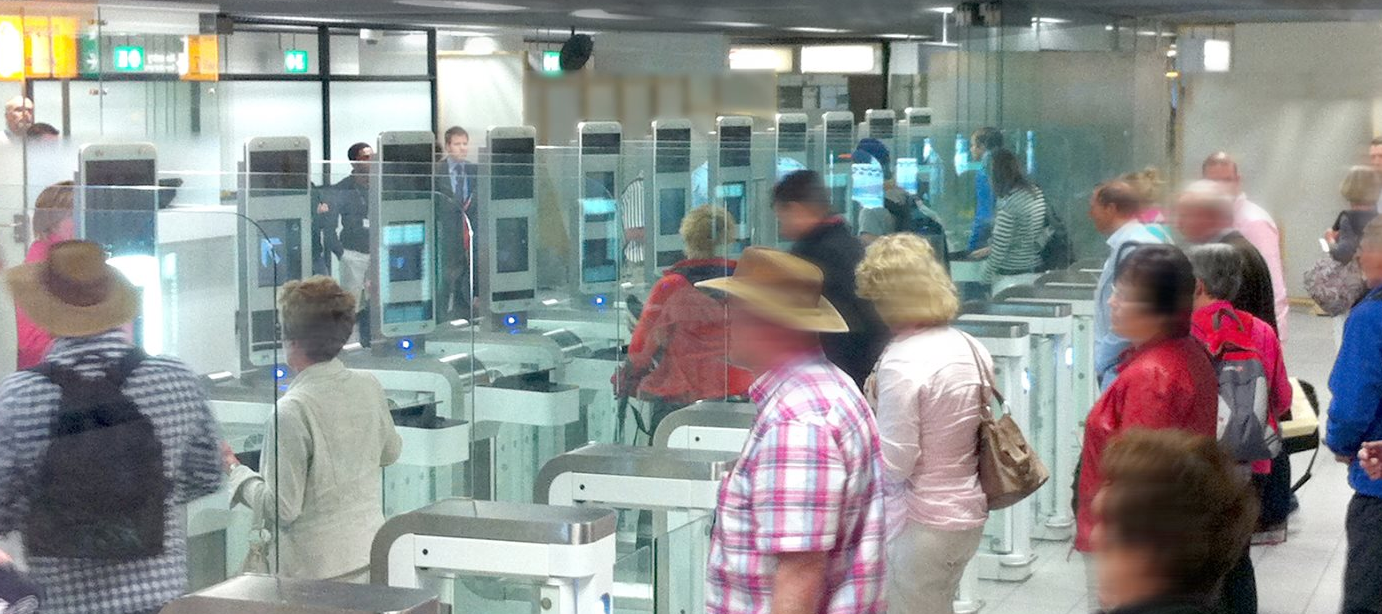
\includegraphics[width=0.8\textwidth]{ch-sistemasABC/images/ch-SistemasABC/ABCsEnElAeropuertoPortugal.png}
    \caption{Sistemas \gls{ABC} en el aeropuerto Humberto Delgado (Liboa, Portugal) \cite{ABC4EUOnline}}
    \label{fig:ABCEnElAeropuerto}
\end{figure}

Las acciones y las comprobaciones que deben realizarse en un control de frontera para autorizar el cruce de un viajero, dependen del tipo de frontera, de los países de origen y de destino, y del propio viajero. Pero, básicamente se resumen en cuatro operaciones que los agentes de frontera en primera linea\footnote{Se conoce como primera linea al área dentro de los puntos de cruce de frontera donde se sitúan los agentes para realizar los controles pertinentes.}, deben realizar, en el menor tiempo posible: 

\begin{itemize}
    \item
    Verificar la autenticidad de la documentación del viajero.
    \item
    Verificar la identidad del viajero contra la identidad almacenada en los documentos que porta.
    \item
    Chequear la autorización del viajero para cruzar la frontera y comprobar que cumple las condiciones de entrada entrada en el país. 
    \item
    Analizar las posibles amenazas de seguridad.
\end{itemize} 

El flujo de viajeros ha ido creciendo constantemente durante los últimos años y la \textit{International Air Transport Association} (\GLS{IATA} \cite{IATAOnline}) estima que para $2025$ habrá unos $887$ millones de viajeros en Europa y $7$ mil millones para $2034$, en todo el mundo \cite{IATA/REVIEW/2016}. Este incremento de viajeros y el uso de nuevas tecnologías para la falsificación de documentos y para la \textit{suplantación de identidades}, deja claro que un enfoque únicamente manual no es suficiente y resulta necesario el uso de sistemas automáticos, como los \textit{Automated Border Control} \GLS{ABC} que complementen el trabajo de los agentes.

Los sistemas \GLS{ABC} son sistemas automáticos o semiautomáticos para la identificación de viajeros en los cruces de frontera. Se basan en la lectura automática de los documentos de viaje y en la verificación biométrica. Deben realizar las mismas comprobaciones en un tiempo igual o menor al de los procesos manuales, permitiendo de este modo: facilitar los cruces, aumentar el flujo de viajeros y mantener los estándares de seguridad, sin necesidad de incrementar el número de guardias de seguridad.

Actualmente, la mayoría de los aeropuertos internacionales disponen de sistemas \GLS{ABC} en sus cruces de frontera (ver Fig. \ref{fig:MapaABCMudialesIATA} ), y también, cada vez es más frecuente encontrar estos sistemas en otro tipo de fronteras, como puertos marítimos o fronteras terrestres (ver Fig. \ref{fig:fronterasConABC}). 

\begin{figure}
    \centering
    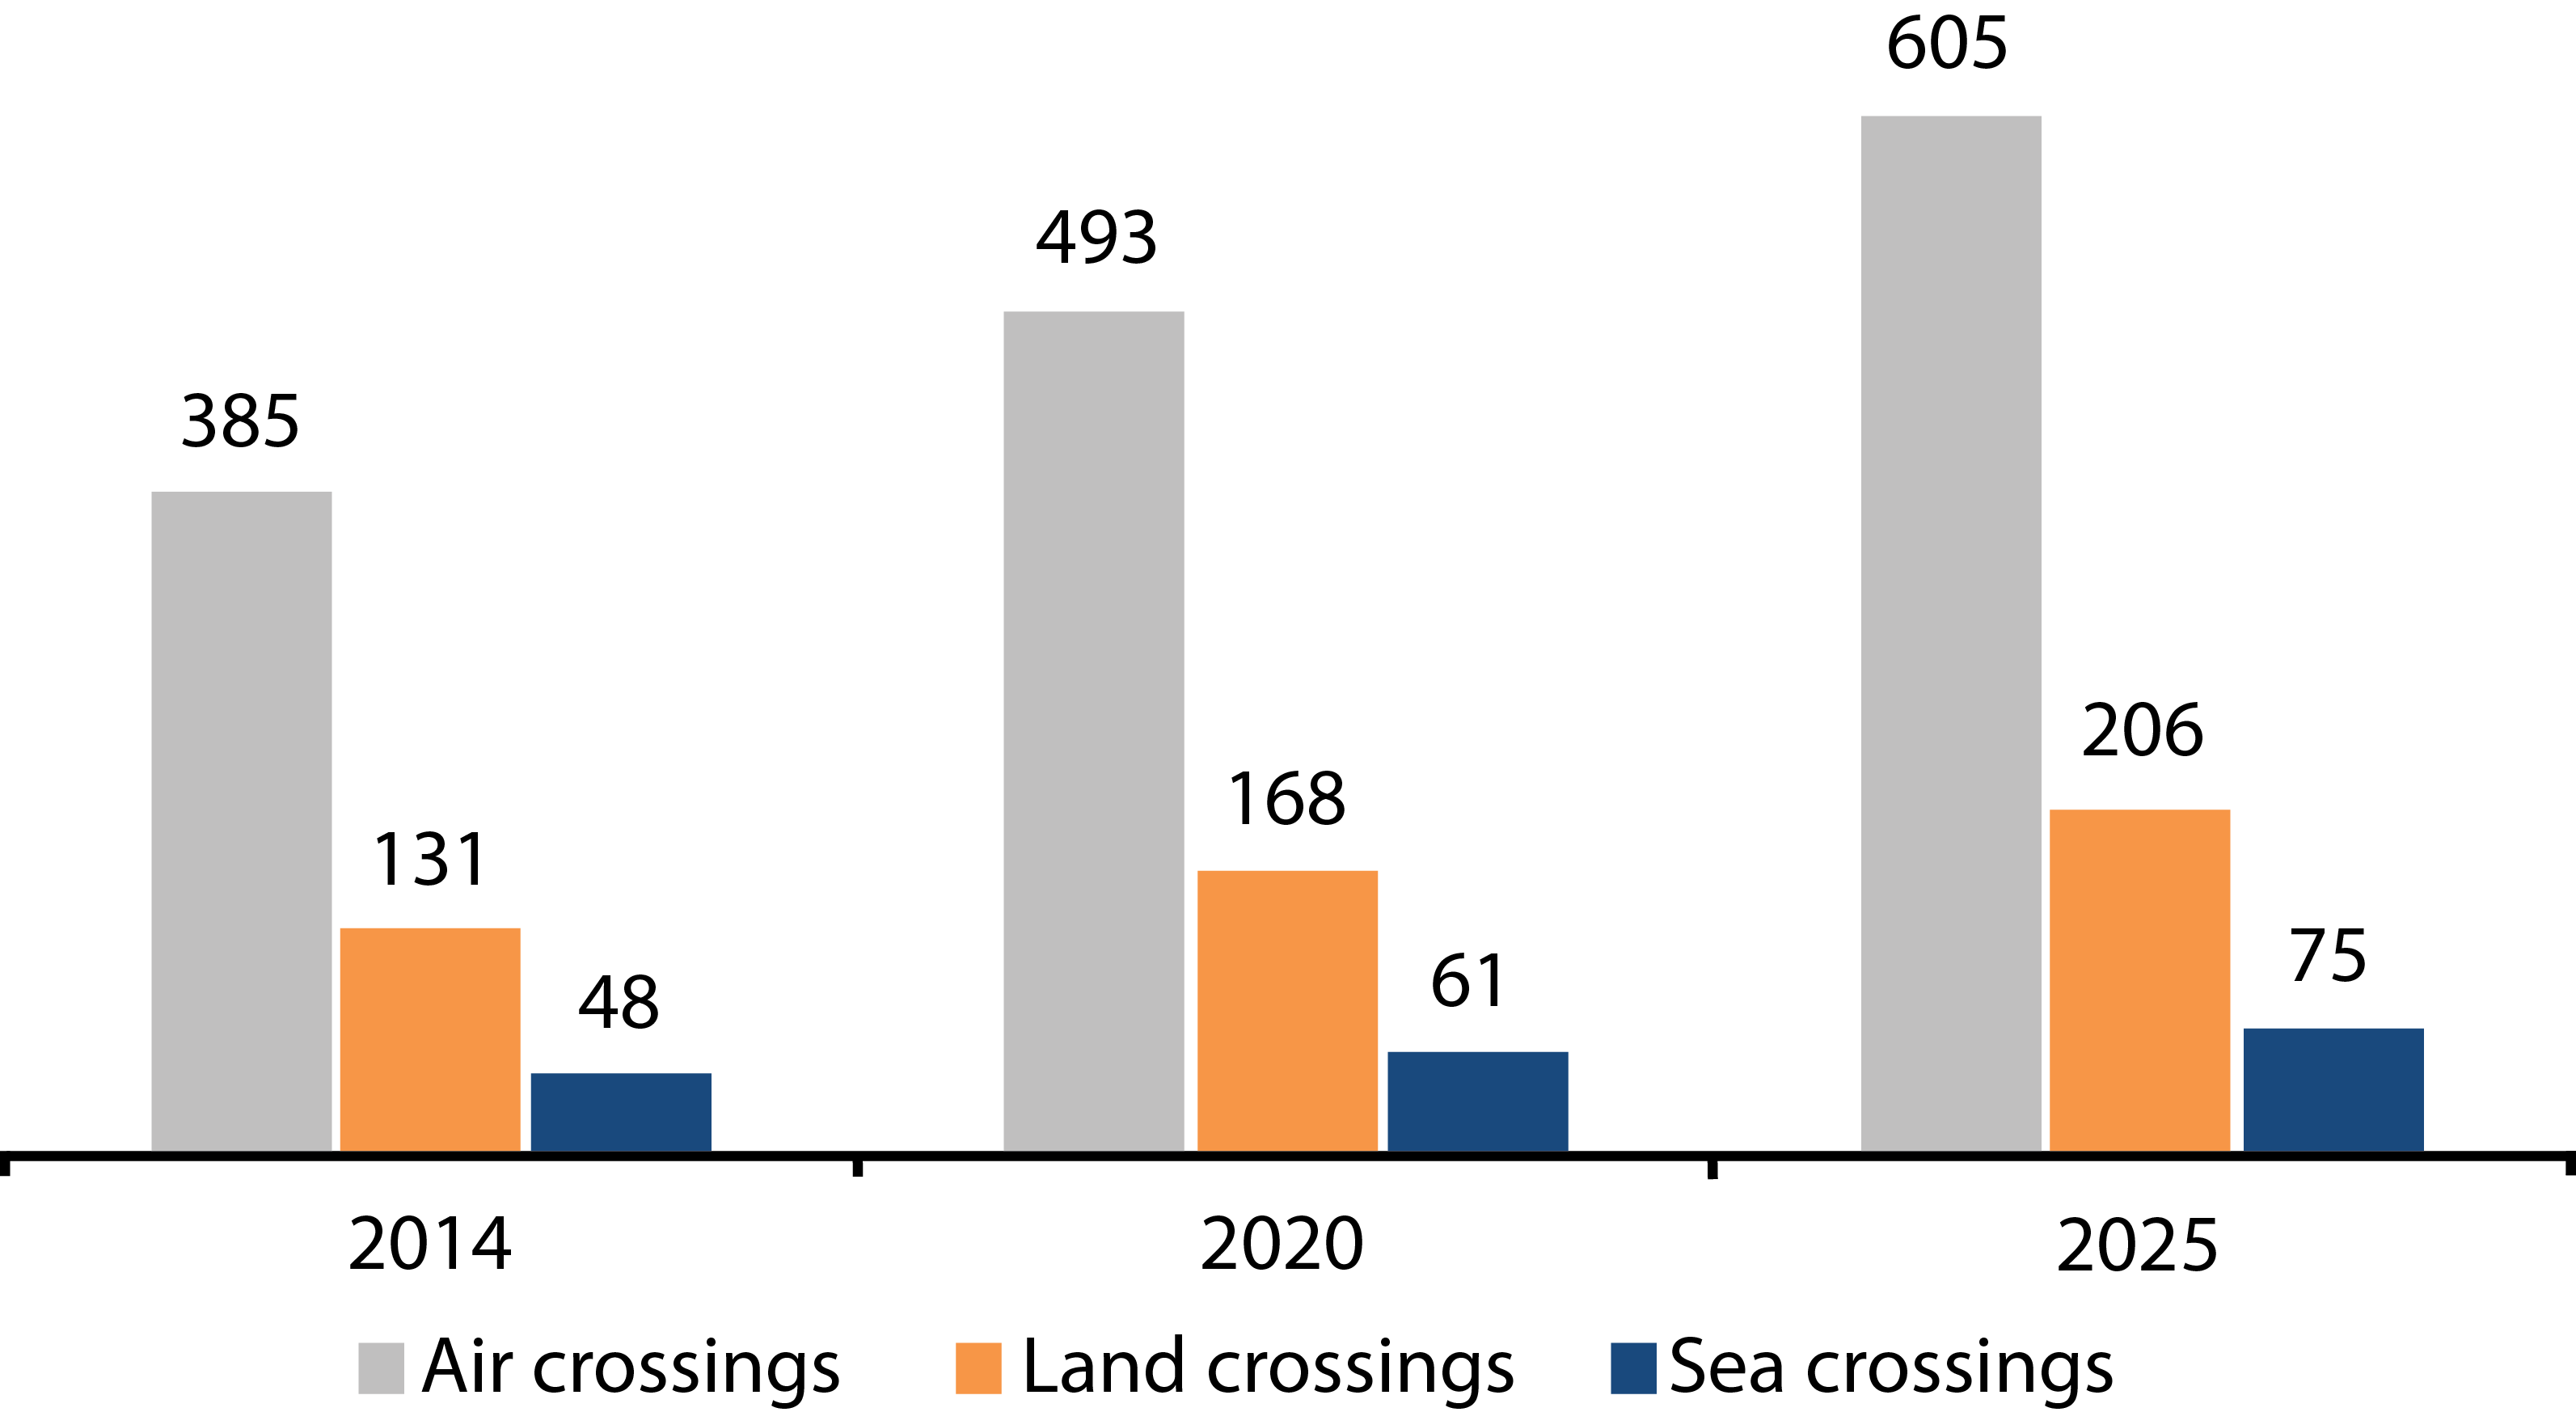
\includegraphics[width=0.7\textwidth]{ch-sistemasABC/images/ch-SistemasABC/ABC_TipoFronteras.png}
    \caption{Sistemas \GLS{ABC} por tipos de fronteras.}
    \label{fig:fronterasConABC}
\end{figure}

\begin{figure}
    \centering
    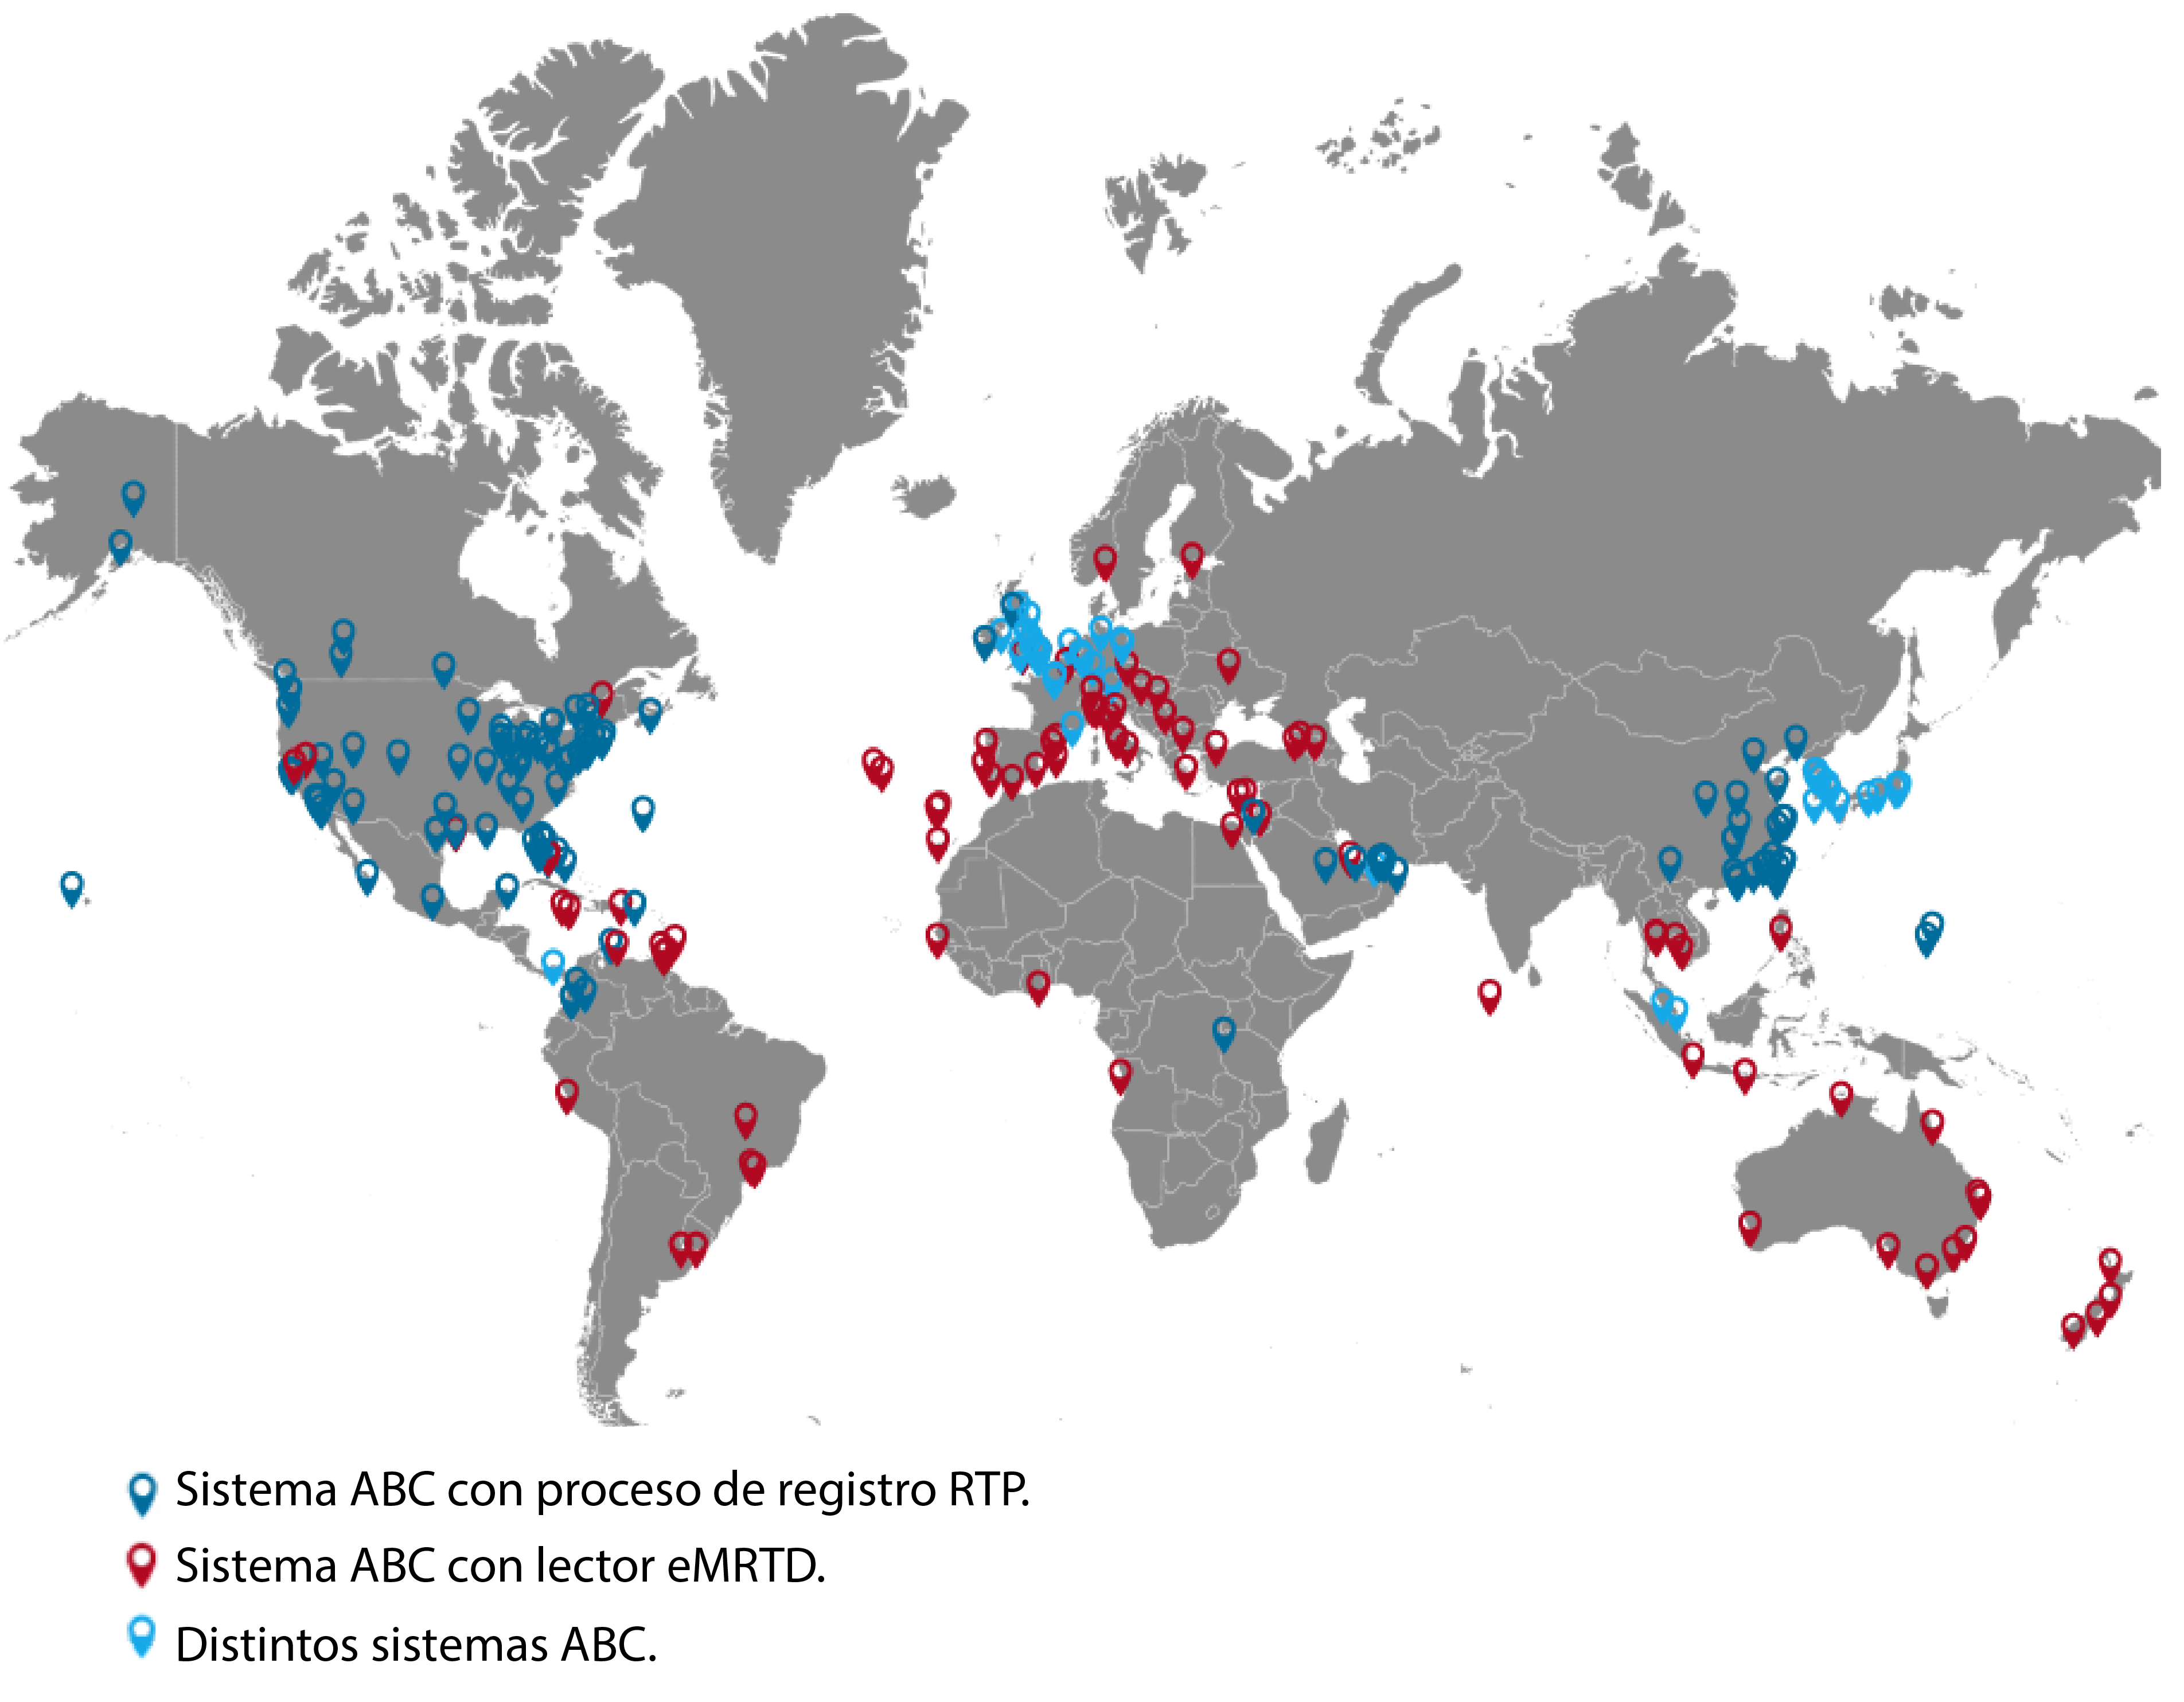
\includegraphics[width=0.8\textwidth]{ch-sistemasABC/images/ch-SistemasABC/AeropuertosConSistemasABCMapaIATA.png}
    \caption{Aeropuertos internacionales con distintos tipos de sistemas \GLS{ABC} en $2019$. \textit{International Air Transport Association} (\GLS{IATA} \cite{IATAOnline}).}
    \label{fig:MapaABCMudialesIATA}
\end{figure}


%%%%%%%%%%%%%%%%%%%%%%%%%%%%%%%%%%%% SISTEMAS ABC:FUNCIONAMIENTO DE LOS SISTEMAS ABC %%%%%%%%%%%%%%%%%%%%%%%%%%%%%%%%%%%%
\subsection{Funcionamiento}\label{sec:funcionamientoABC}

Las tareas fundamentales a realizar en un cruce de fronteras con sistemas automáticos consisten en: El escaneo del pasaporte, la autenticación de la documentación de viajero, la comprobación de su idoneidad para cruzar la frontera y la verificación de su información biométrica. Además de éstas, existen otras tareas no automáticas y una tarea fundamental que involucra a todas las demás que es controlar la seguridad de todo el proceso.

\begin{itemize}
    \item 
    \textbf{Escaneo del pasaporte} 
    
    El viajero debe portar un \textit{Electronic machine-readable travel document} (\gls{eMRTD}), legible por el sistema y que cumpla con las especificaciones dadas para este tipo de documentos por la \textit{International Civil Aviation Organization} (\GLS{ICAO} \cite{ICAOOnline}) en el informe \GLS{ICAO} Doc $9303$ \cite{doc20069303}. El \gls{eMRTD}, habitualmente un \textit{Electronic Passport} \gls{e-passport}, debe incluir la información biométrica del viajero portador \footnote{Para más información sobre los documentos de viaje es posible consultar en \GLS{ICAO}-Doc $9303$ \cite{doc20069303} y el Apéndice \ref{apendix:DocDeViaje} donde se detallan los documentos soportados por los sistemas \GLS{ABC}.}.
    
    El viajero debe colocar el documento de viaje, en el lector de documentos por la hoja de datos de forma que quede visible la \textit{Machine-Readable Zone} (\GLS{MRZ}, Figura \ref{fig:HojaDatos_MRZ} b)). 
    
    En caso de que el viajero no porte documentación valida o ésta no pueda ser leída, el viajero será rechazado.
    
    \item
    \textbf{Autenticación y verificación de la documentación}
    
    Tras escanear el documento es necesario comprobar su \textbf{autenticidad} y confirmar que sean \textbf{documentos válidos y genuinos}. 
    
    Con la imagen capturada del documento se realiza un proceso de lectura automático \textit{Optical Character Recognition} (\GLS{OCR}) sobre la \GLS{MRZ}, donde se leen algunos datos biográficos del viajero. Y de forma simultanea, mediante radio-frecuencia se extrae la información almacenada en el chip \GLS{RFID} integrado en el documento \gls{eMRTD}. 
    
    Para autenticar los documentos, la información visual leída se contrasta con la extraída del chip.

    Además de autenticar la identidad de la documentación, también se examinan las medidas de seguridad y de antifalsificación que tienen los pasaportes (para ver algunas de estas medidas ver la Figura \ref{fig:MarcasSeguridadDocumentos}, en el Apéndice  \ref{apendix:DocDeViaje}).
    
    \item
    \textbf{Comprobación de la información biométrica}
    
    Se realiza una verificación de la identidad del viajero mediante sus datos biométricos. Dependiendo de los sistemas y del tipo de documentación se pueden usar unos rasgos biométricos u otros. Los rasgos que más comúnmente se capturan en los sistemas \GLS{ABC} son la cara, para biometría \gls{facial}, huellas dactilares en la biometría \gls{dactilar} o los ojos en la \textbf{biometría del \gls{iris}}. (Por ejemplo, el sistema puede capturar una imagen en vivo de la cara del viajero y compararla con la cara impresa en el pasaporte o con la almacenada en el chip).
    
    \item
    \textbf{Idoneidad del viajero}
    
    Además de controlar la autenticidad de los documentos y la identidad del viajero, también se debe comprobar la elegibilidad y la autorización del viajero para cruzar la frontera. Esto depende del viajero en sí y de las reglas y los requisitos de cada país.  
    Para decidir si el viajero es apto o no para cruzar la frontera se requiere consultar bases de datos y registros centrales a los que los sistemas \GLS{ABC} deben tener acceso, como : \textit{Schengen Information System} (\textbf{\GLS{SIS}}) en las fronteras de \GLS{EU}; \textit{Visa Information System} (\textbf{\GLS{VIS}}), para el control de visados; National \GLS{PKD}, con los encriptados del chip, especificos en cada pais; \textit{Vehicle Registration Certificate} (\GLS{VRC}), en algunas fronteras terrestres; \GLS{AFIS-ABIS}, para el registro de huellas dactilares; etc. % \Gls{INTERPOL}, \textit{Opt.national}.

    \item
    \textbf{Tareas no automatizadas}
    
    En algunos casos, para determinados viajeros, los controles automáticos de los \GLS{ABC} no son son suficientes y se requieren otros procesos que por ahora se deben realizar manualmente como por ejemplo, el estampado del pasaporte o alguna de las comprobaciones del visado (entrevista de los agentes de seguridad). 

    \item
    \textbf{Seguridad}
    
    Los sistemas deben de garantizar la seguridad en todos los procesos y sólo en el caso de que todos procesos del sistema \GLS{ABC} se realicen de forma satisfactoria el viajero podrá cruzar la frontera. Si se produce algún fallo los agentes de seguridad que controlan los sistemas de forma remota, se harán cargo de la situación. También en el caso de que algún viajero no pueda usar los sistemas automáticos debe ser dirigido a los controles manuales.

\end{itemize}


%%%%%%%%%%%%%%%%%%%%%%%%%%%%%%%%%%%% SISTEMAS ABC:ARQUITECTURA %%%%%%%%%%%%%%%%%%%%%%%%%%%%%%%%%%%%
\subsection{Arquitectura}\label{sec:AquitecturaABC}

\begin{figure}
    \centering
    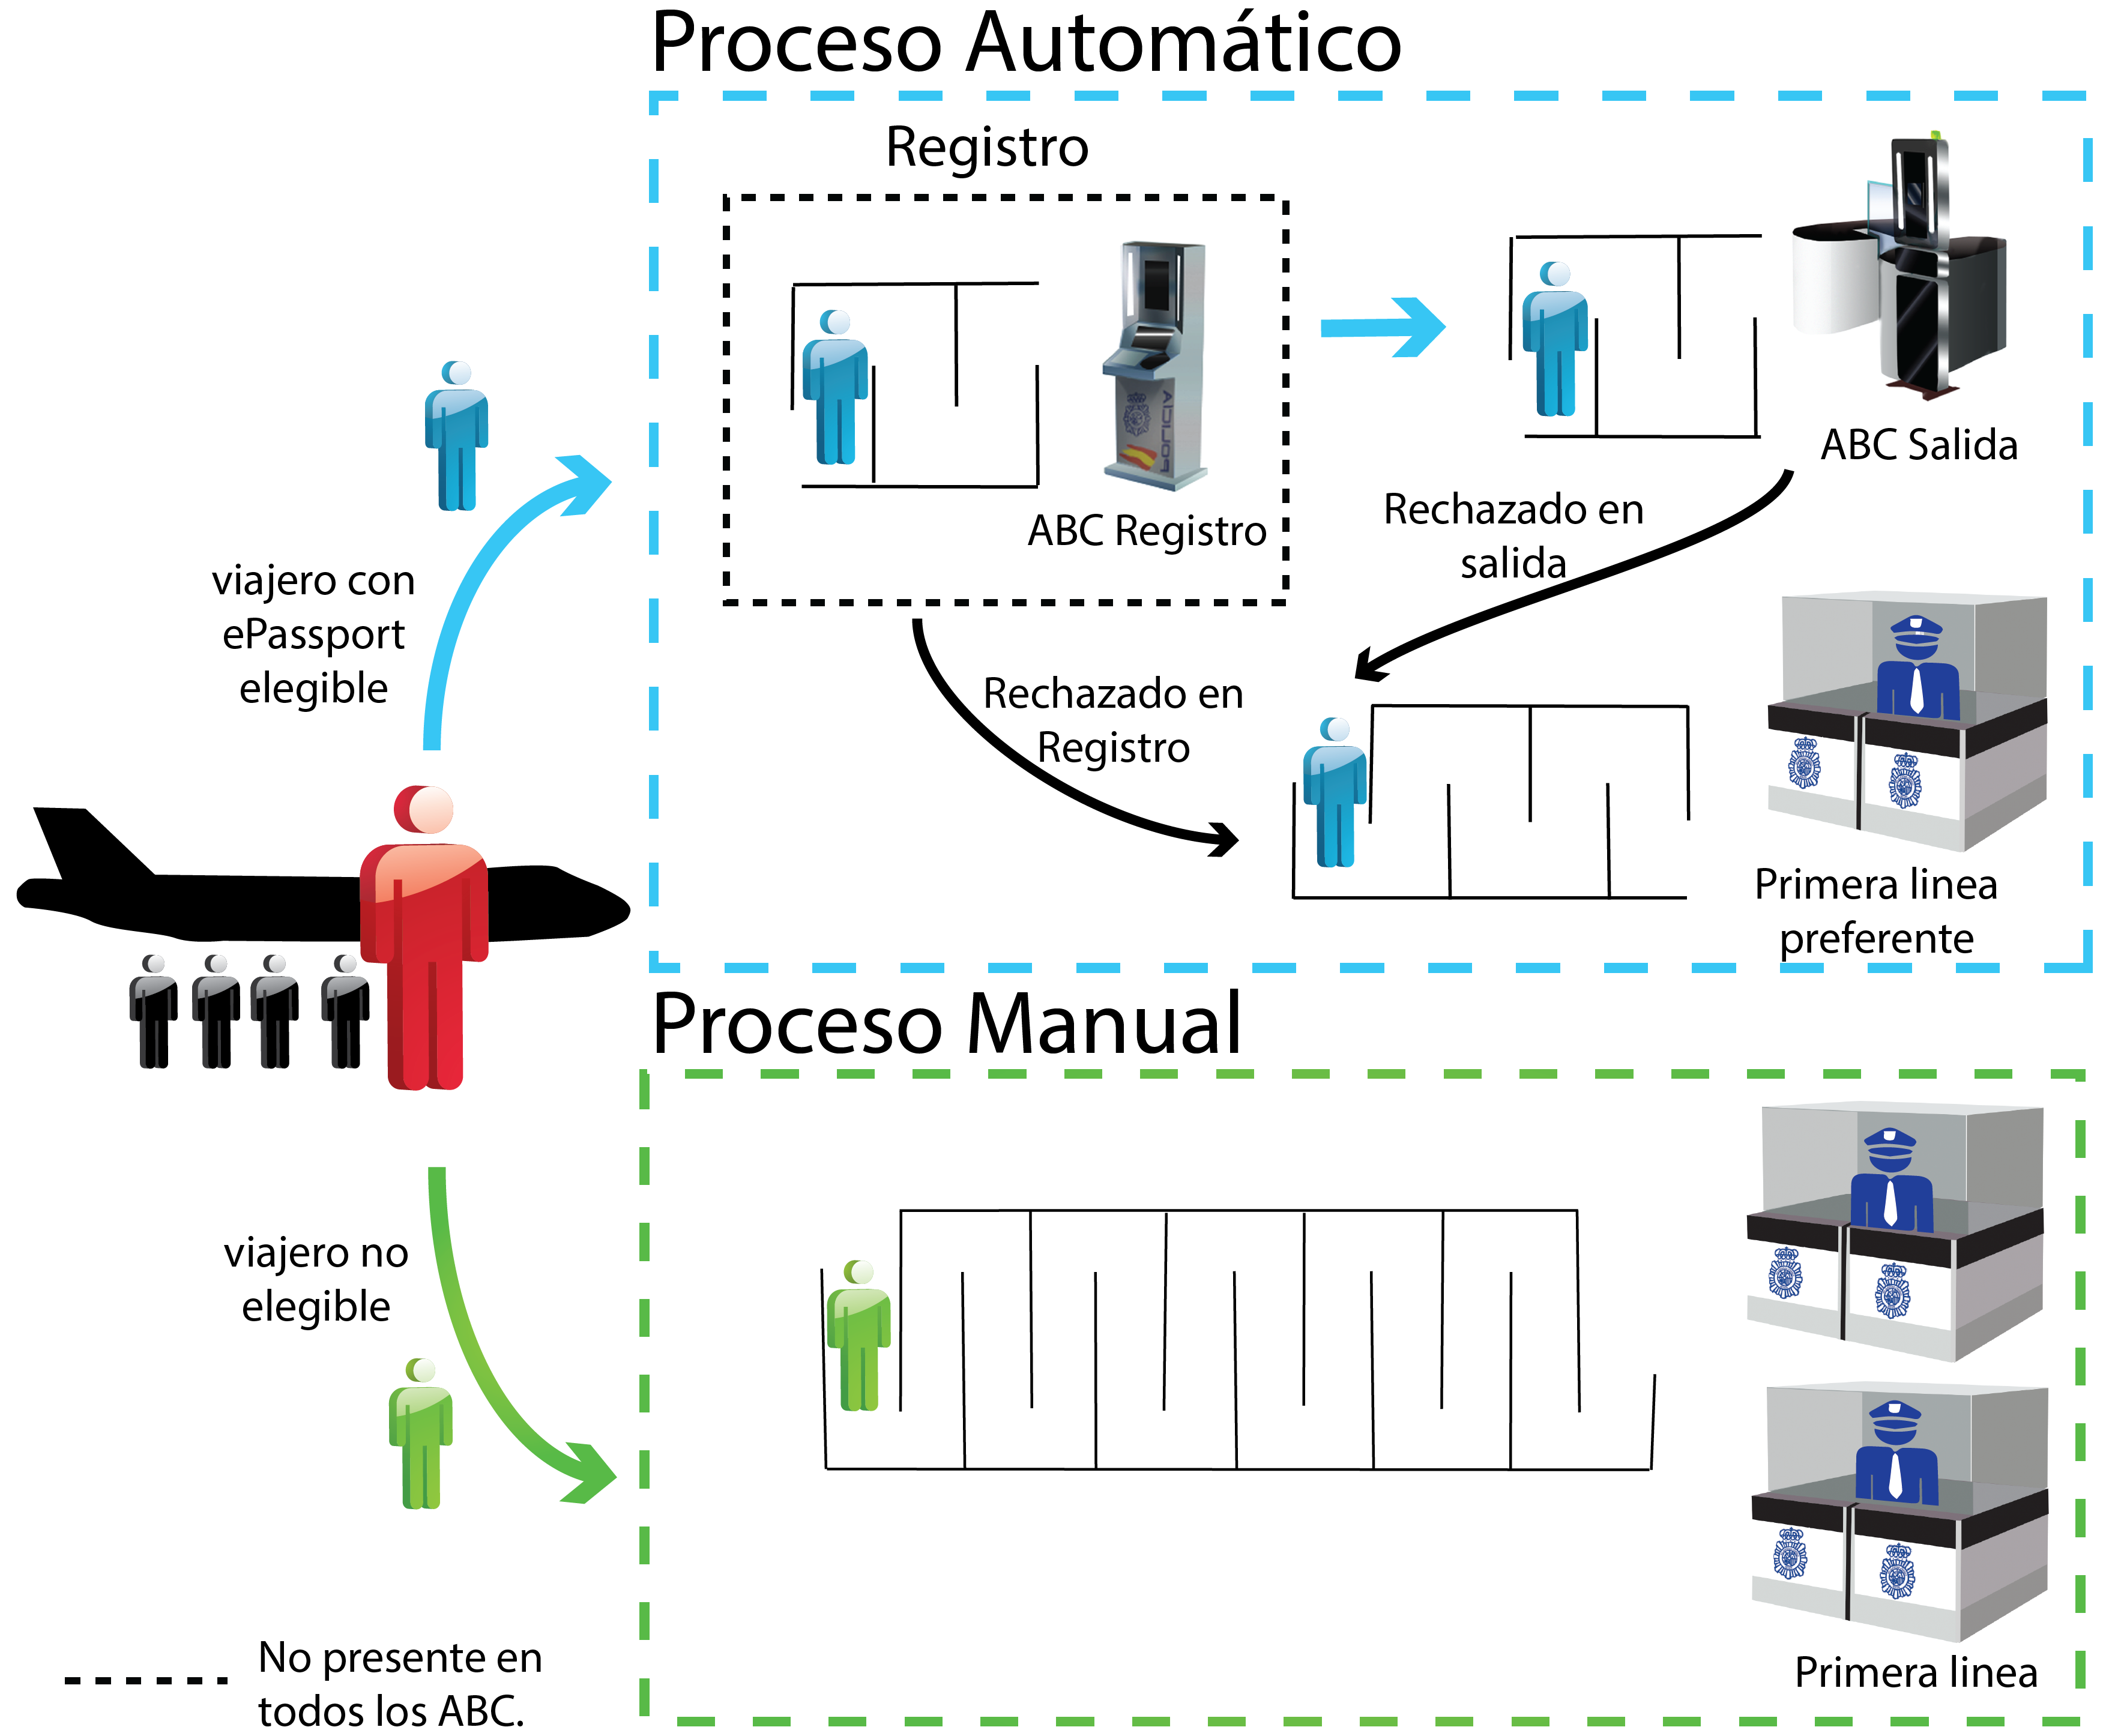
\includegraphics[width=1\textwidth]{ch-sistemasABC/images/ch-SistemasABC/ArquitecturaEnAeropuerto.png}
    \caption{Esquema aeropuerto con sistemas \GLS{ABC}s \cite{labati2016biometric}.}
    \label{fig:EsquemaAeropuerto}
\end{figure}


Los sistemas \GLS{ABC} tienen una arquitectura física y una arquitectura lógica. Cada \GLS{ABC} esta compuesto por uno o varios dispositivos que son su arquitectura física, sobre la que se implementan las tareas de un conjunto de subsistemas que interactuaban entre si y que integran la arquitectura lógica del sistema.

Dependiendo de como se distribuya la arquitectura lógica en los dispositivos físicos, se distinguen distintos tipo de \textbf{topologías de sistemas \GLS{ABC}}.


%%%%%%%%%%%%%%%%%%%%%%%%%%%%%%%%%%%% SISTEMAS ABC:ARQUITECTURA LOGICA %%%%%%%%%%%%%%%%%%%%%%%%%%%%%%%%%%%%
\subsubsection{Arquitectura lógica}\label{subsec:ArquitecturaLogicaABC}

\begin{figure}
    \centering
    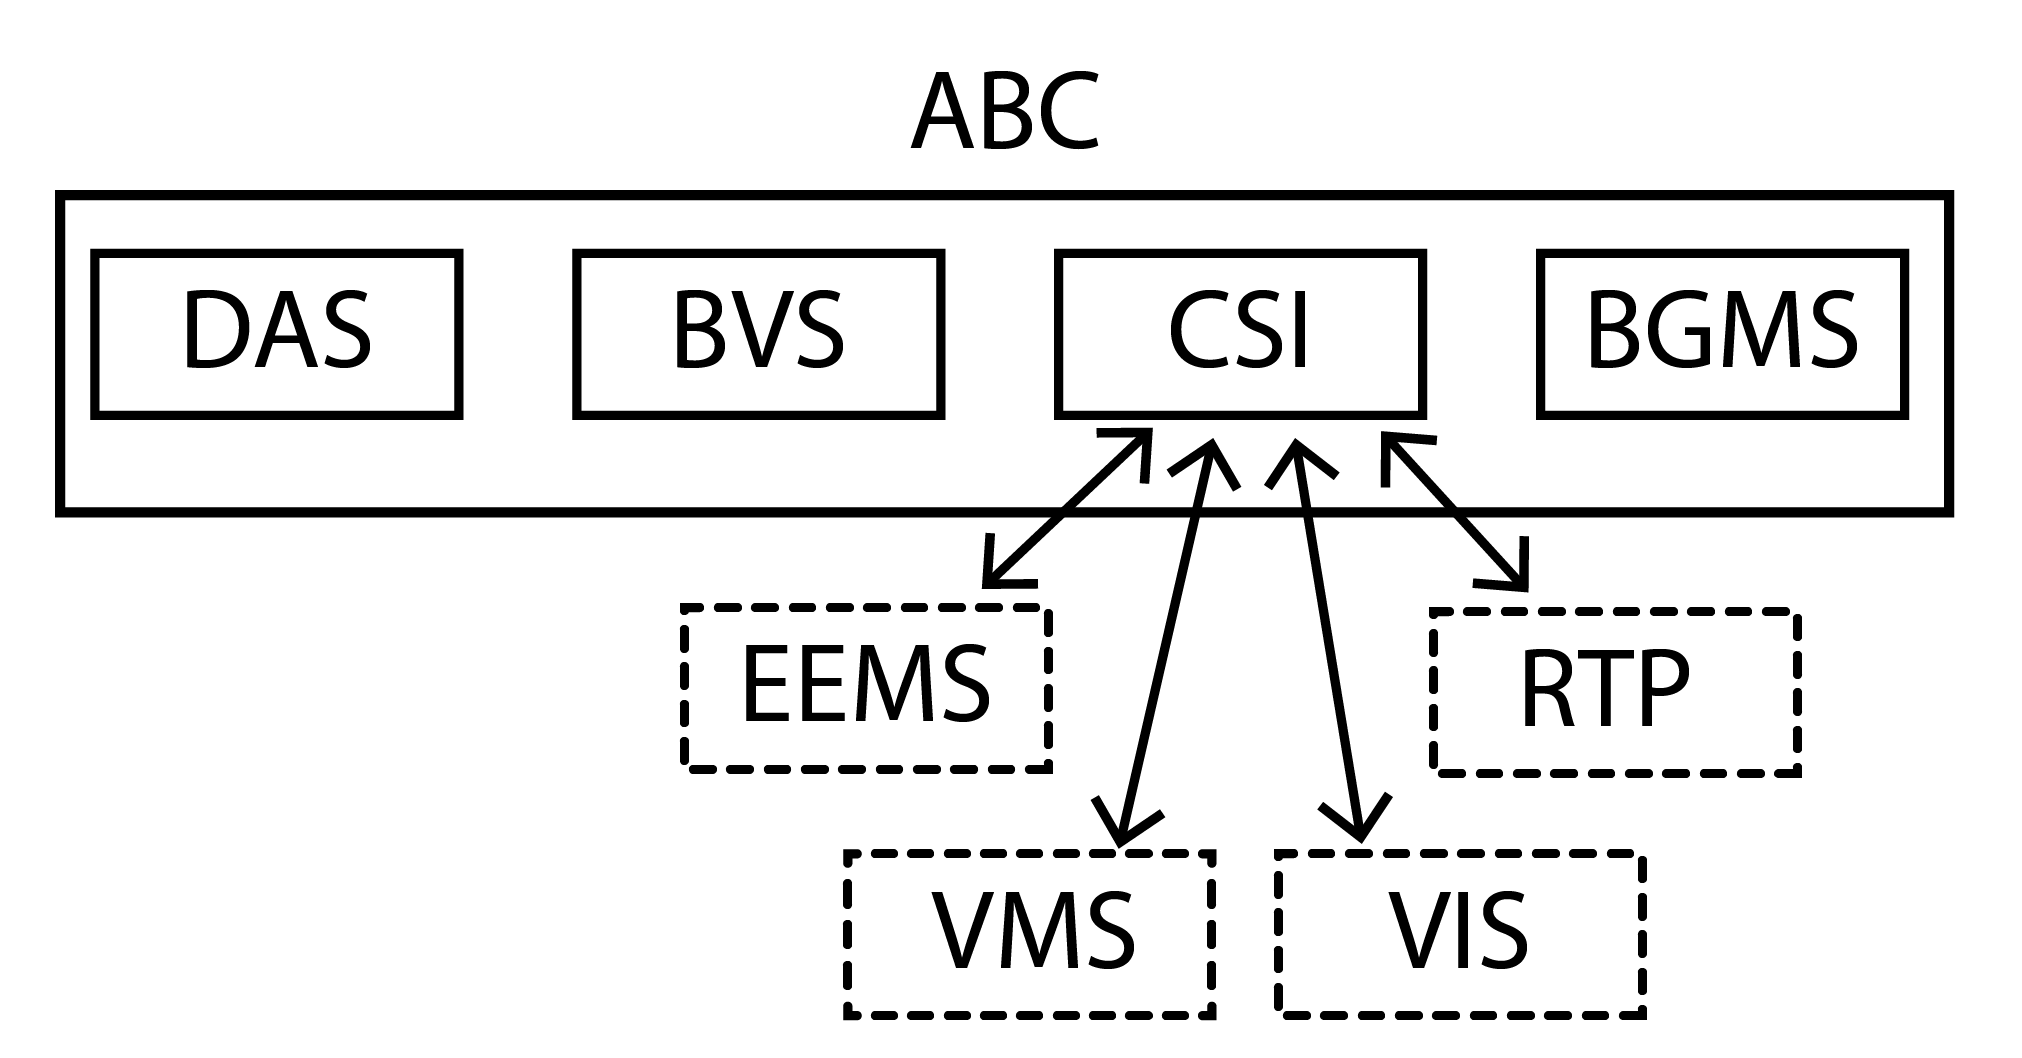
\includegraphics[width=0.7\textwidth]{ch-sistemasABC/images/ch-SistemasABC/SUBSISTEMAS_ABC.png}
    \caption{Subsistemas y servicios externos de de un sistema \GLS{ABC} \cite{labati2016biometric}.}
    \label{fig:SubsistemasABC}
\end{figure}

La arquitectura lógica de los sistemas se encarga de la realización de dos procesos principales: \textit{Register Traveller Program} (\textbf{\GLS{RTP}}) y \textit{Entry/Exit System} (\textbf{\GLS{EES}}). Y para ello cuenta con una serie de \textbf{subsistemas} que además de comunicarse entre ellos, interactúan con una serie de \textbf{servicios externos} (ver Fig. \ref{fig:SubsistemasABC}).

Para garantizar una correcta comunicación entre los distintos módulos y con los sistemas externos, es necesario que los \GLS{ABC} sigan una serie de especificaciones en sus protocolos de comunicación, interfaces y formatos de intercambio \footnote{\GLS{ISO}/\GLS{IEC} 19794, define un estándar para el intercambio de información entre los distintos módulos de un sistema biométrico.}.
    
Seguir estos estándares también permite una mayor flexibilidad y modularidad en los sistemas, ya que permite modificar un modulo del sistema sin cambiar el sistema completo.

\medskip
\textbf{Procesos}

Existen distintos protocolos, dependiendo del tipo de viajero, del país de origen, del tiempo de estancia en país de destino, etc. Pero los procesos comunes a todos los \GLS{ABC} son: \GLS{RTP} y \GLS{EES}. 

\begin{itemize}
    \item 
    \textbf{\GLS{RTP}}
    
    Se verifica la identidad del viajero y su adecuación para cruzar la frontera atendiendo a la información almacenada en su documentación. Este proceso puede realizarse de forma previa al viaje, en el caso de viajeros frecuentes o registrados con anterioridad, o bien ya en el aeropuerto, normalmente en dispositivos \gls{e-kiosk}. La información biométrica del viajero, capturada en el momento (\gls{vivo}) se verifica con la almacenada en sus documentos de viaje.
    
    \item 
    \textbf{\GLS{EES}}
    
    Este proceso se realiza en dispositivos \gls{e-gate}, ya en el cruce de fronteras.
    Y consiste en el emparejamiento entre el la información biométrica registrada y los datos capturados \textit{in-vivo} de viejo en el momento del cruce. Es decir, la información biométrica es nuevamente capturadas y se compara con la capturada en el proceso \GLS{RTP}.
\end{itemize}

\medskip
\textbf{Subsistemas}

Para la realización de los procesos \GLS{RTP} y \GLS{EES} intervienen una serie de subsistemas dentro del sistema \GLS{ABC}:

\begin{itemize}
    \item 
    \textbf{DAS} (\textit{Document Authentication System}): Evalúa la validez y la legitimidad de la documentación del viajero. Además de verificar las marcas de autenticidad de los documentos, lee la zona legible del documento \GLS{MRZ} y la información almacenada en el chip en caso de que sea un \gls{eMRTD}. 
    
    \item 
    \textbf{\GLS{BVS}} (\textit{Biometric Verification System}): Se encarga de verificar la información biométrica del viajero capturada en el sistema (\gls{vivo}), con la leída en la documentación. 
    
    \item 
    \textbf{CSI} (\textit{Control System Interface}): Gestiona la comunicación con las interfaces externas. Por ejemplo, para comprobar la idoneidad del viajero. Dependiendo de la normativa de cada país los \GLS{ABC} se conectan a unos servicios u a otros. 
    
    \item
    \textbf{BGMS} (\textit{Border Guard Maintenance System}): Incluye las tareas de control y de monitorización de los agentes de frontera. 
\end{itemize}

\textbf{Servicios externos}

\begin{itemize}
    \item 
    \textbf{VMS} (\textit{Visa Management System}): 
    
    Se encarga de las gestiones con el sistema \GLS{VIS} (\textit{Visa Information System}).
    
    Base de datos con el toda la información sobre el visado del viajero\footnote{El parlamento europeo en $2008$ definió la información del sistema \GLS{VIS} para todos los países de la Unión:  https://eur-lex.europa.eu/legal-content/EN/TXT/?uri=CELEX\%3A32008R0767.} : Tipo de visado, información personal del viajero, biométrica y biográfica, información del viaje, fecha de entrada, duración del visado.
    
    Los sistemas \GLS{ABC} se comunican con este sistema mediante el número de visa, un número identificador y los datos biométricos del viajero.

    \item 
    \textbf{RTP} (\textit{Registered Traveller Programme}).
    
    Base de datos con la información ciertos viajeros que se han registrado previamente en sistema\footnote{La Unión Europea está analizando este tipo de pre-registro para si fronteras. Diferentes proyectos en el marco FP$7$, como \GLS{ABC4EU} o \GLS{FastPass}, estudian este tipo de procesos.}. El registro previo es voluntario y simplifica un posterior cruce de fronteras, mejorando la seguridad y reduciendo el tiempo del proceso. 
    
    El registro previo está pensado para viajero que por razones laborales o familiares viajan frecuentemente a un determinado país.
    
    El proceso de \GLS{RTP} involucra la captura de la información biométrica del viajero.   
    
    
    \item 
    \textbf{EEMS} (\textit{Entry/Exit Management System}):
    
    Se encarga de las gestiones con el sistema \GLS{EES} (\textit{Entry/Exit System}).
    
    Base de datos que almacena la información del los viajero que cruzan el cruce de fronteras.
    
    Rechaza el antiguo estampado del sello en los documentos.
    
    Almacena información biométrica del viajero.
    
    Permite comprobar a los agentes si lo viajeros han sobrepasado el tiempo de estancia en el país.
    
    Permite a las naciones controlar el flujo de migrantes.
    
    \item 
    \textbf{\GLS{SIS}} (\textit{Schengen Information System}):
    
    Sistema especifico para los viajeros de la Unión Europea (\GLS{EU}). Contienen datos biométricos, como la cara o las huellas dactilares. También contiene información de las agencias de seguridad europeas sobre personas vulnerables y personas peligrosas.  
    
    \item 
    \textbf{\GLS{ETIAS}} (\textit{European Travel Information and Authorisation System}):
    
    Sistema especifico de pre-registro para \GLS{TCNVE} en el área \Gls{Schengen}. Aprobada por la en en $2018$ y comienza a ser operativa en $2022$ \cite{union2018directiveETIAS}.
    
    \item 
    \textbf{\GLS{FADO}} (\textit{False and Authentic Documents Online}):
    
    Base de datos con el formato de los pasaportes originales de cada país e información sobre tipos de falsificaciones en documentos de viaje.
    
\end{itemize}

%%%%%%%%%%%%%%%%%%%%%%%%%%%%%%%%%%%% SISTEMAS ABC:ARQUITECTURA FISICA %%%%%%%%%%%%%%%%%%%%%%%%%%%%%%%%%%%%
\subsubsection{Arquitectura física}\label{subsec:ArquitecturaFisicaABC}

Los sistemas \GLS{ABC} pueden estar compuestos de varios dispositivos y sensores con los que el viajero interactúa para realizar los distintos los procesos (ver Fig. \ref{fig:ElementosFisicosABC}). Dentro de estos dispositivos se pueden encontrar:

\begin{figure}
    \centering
    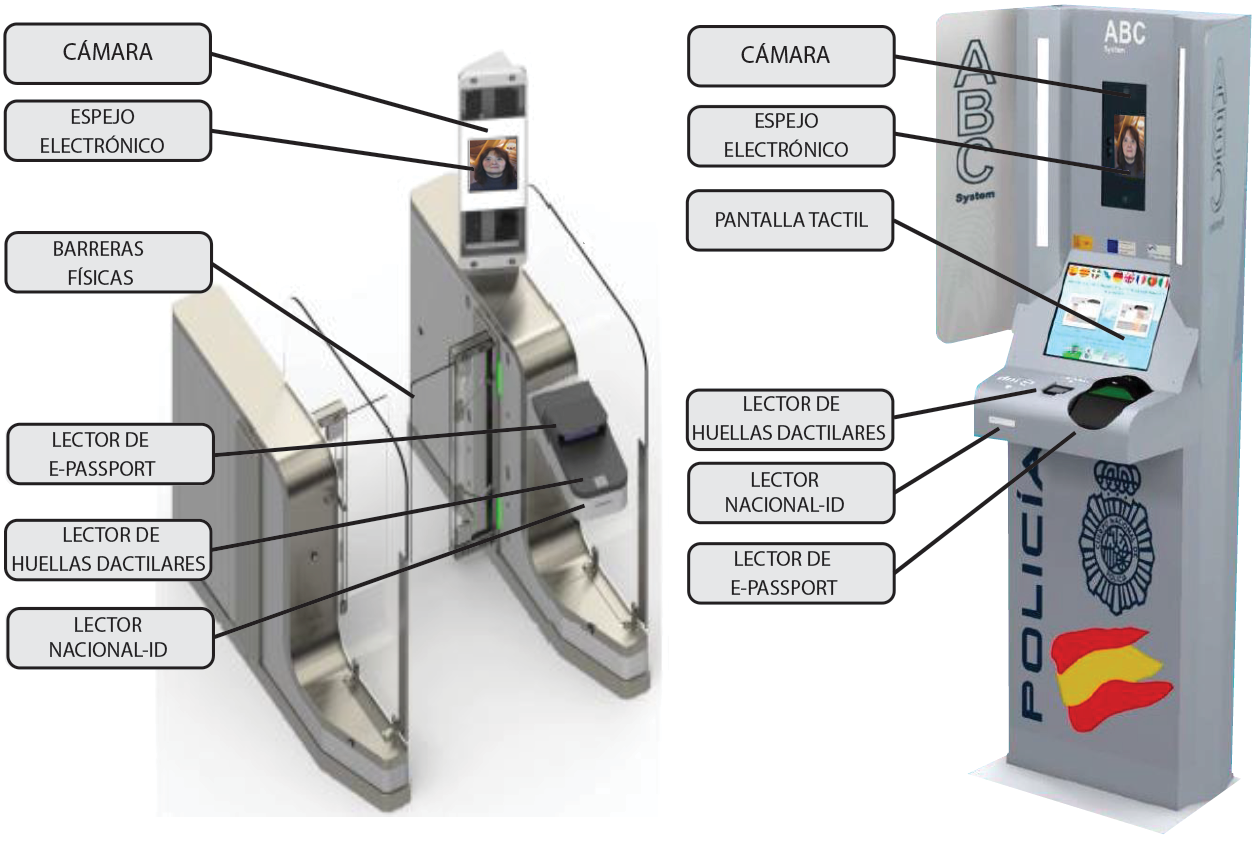
\includegraphics[width=1\textwidth]{ch-sistemasABC/images/ch-SistemasABC/ELEMENTOS_FISICOS_SISTEMAS_ABC.png}
    \caption{Componentes físicos más comunes de los dispositivo \GLS{ABC} (\GLS{ICAO}\cite{ICAOOnline})}
    \label{fig:ElementosFisicosABC}
\end{figure}

\begin{itemize}
\item 
\textbf{Barreras físicas}, que pueden ser una o varias.

\item
\textbf{Lector de documentos}, preparado para la lectura óptica de los documentos y para la lectura por radiofrecuencia de chip en el caso de documentos \gls{eMRTD}.

\item
\textbf{Dispositivos de captura biométrica}: Cámaras, lectores de huellas dactilares u otro tipo de sensores.

\item
\textbf{Dispositivos para la interacción con el usuario}: Monitores, botones, señales luminosas o altavoces.

\item
\textbf{Sistemas de proceso} donde se ejecuten las distintas tareas. 

\item
\textbf{Sistemas de comunicaciones}: Controladores, conexiones, hubs, etc.

\item
\textbf{Sensores y cámaras de vigilancia} para el correcto funcionamiento del sistema: Detectar objetos abandonados, circuitos de videovigilancia o detectar varios viajeros dentro del dispositivo, etc.  

\item
Una \textbf{estación de control} para que los operadores monitoricen y gestionen de forma remota los sistemas .
\end{itemize}

Para lo sistemas que están instalados en el exterior también deben considerarse elementos para proteger los sistemas de las condiciones climáticas y de actos vandálicos: Puertas protectoras, cerraduras, fijaciones, etc.


%%%%%%%%%%%%%%%%%%%%%%%%%%%%%%%% SISTEMAS ABC:TOPOLOGIAS DE ABC %%%%%%%%%%%%%%%%%%%%%%%%%%%%%%%%%%%%%%%%%
\subsubsection{Topologías}\label{subsec:Topologias}

Dependiendo de la disposición de los dispositivos físicos y de las tareas que se realizan en cada dispositivo se pueden considerar distintas topologías de sistemas \GLS{ABC}.

Si la validación de los documentos y la verificación de la identidad del viajero, se realizan en un único proceso el sistema tiene una topología \textit{<<One Step>>}, mientras que si esas tareas se desdoblan en los dos procesos (\GLS{RTP} y \GLS{EES}) tendrá una topología \textit{<<Two Step>>}. Los sistemas \GLS{ABC} con topología de dos pasos puede tratarse a su vez, de una topología \textit{<<Integrated Two Step>>} o \textit{<<Segregated Two Step>>}.    

\begin{figure}
    \centering
    
\includegraphics[width=0.8\textwidth]{ch-sistemasABC/images/ch-SistemasABC/topologiasABC.png}
    \caption{(a). Topología \GLS{ABC} \textit{<<One Step>>}. (b). Topología \GLS{ABC} \textit{<<Integrated Two Step>>}. (c). Topología \GLS{ABC} \textit{<<Segregated Two Step>>}. \cite{FRONTEX2016OpeReport}}
    \label{fig:TopologiasABC}
\end{figure}

\medskip
\textbf{Topología \textit{<<One Step>>}}
\medskip

En la topología \textit{<<One Step>>} los procesos de \GLS{RTP} y \GLS{EES} se fusionan en un único proceso en el que se realiza la identificación del viajero en el mismo momento en el que éste cruza la frontera (Figura \ref{fig:TopologiasABC} (a)). Verificación y seguridad se realizan en una única transición. 

Los dispositivos con este tipo de topologías suelen ser \gls{e-gate} de tipo \gls{mantrap} (Figura \ref{fig:dispositivosABCEstaticos} b)) que no permiten el paso hasta que no se ha realizado correctamente la identificación. Aun así  son más rápidos ya que pueden realizar algunas acciones en paralelo. Por ejemplo, capturar los datos biométricos del viajero mientras se consulta su elegibilidad con los datos biográficos.

\medskip
\textbf{Topología \textit{<<Two Step>>}}
\medskip

En las topologías \textit{Two Steps} los procesos \GLS{RTP} y \GLS{EES} están bien diferenciados. Primero el viajero es registrado y a continuación se verifica su información biométrica antes de permitir el cruce. 

Dependiendo de si los procesos se realizan en un mismo dispositivo o en dos, se distingue entre topologías \textit{<<Integrated Two Steps>>} (Figura \ref{fig:TopologiasABC} (a)) y \textit{<<Segregated Two Step>>} (Figura \ref{fig:TopologiasABC} (b)).

\begin{itemize}
    \item 
    \textbf{Topología \textit{<<Integrated Two Step>>}}
    
    La verificación de documentación y la comprobación de la idoneidad del viajero se realiza en una etapa, necesaria para proceder a una segunda etapa en la que se realiza la verificación biométrica y otras operaciones de control.
    
    Los procesos de \GLS{RTP} y \GLS{EES} se realizan en el mismo dispositivo, habitualmente un \gls{mantrap}, como en las topologías \textit{<<One Step>>}
    
    \item
    \textbf{Topología \textit{<<Segregated Two Step>>}}
    
    El proceso \GLS{RTP} se realiza en un dispositivo, habitualmente un \gls{e-kiosk} (Figura \ref{fig:dispositivosABCEstaticos} (a)) y el \GLS{EES} en otro dispositivo distinto una \gls{e-gate} (Figura \ref{fig:dispositivosABCEstaticos} (c)).    
    
    Una primera etapa en la que se realiza la verificación del viajero y la captura de los datos biométricos del viajero, que generan un \textit{\gls{token}} \footnote{Alguna publicaciones llaman a esta biometría pre-pregistrada \gls{biometria} <<táctica>>.} con el cual, en una segunda etapa, se realizará una nueva verificación, con los datos del viajero que desea cruzar la frontera.

    Los sistemas segregados permiten optimizar el espacio y el tiempo respecto de las topologías con procesos integrados, pero también pueden confundir a los viajero inexpertos que pueden no entender claramente por que el proceso esta dividido en dos pasos. También requiere más mantenimiento al tratarse de dos dispositivos.
\end{itemize}

%%%%%%%%%%%%%%%%%%%%%%%%%%%%%%%%%%% SISTEMAS ABC:TIPOS DE ABC %%%%%%%%%%%%%%%%%%%%%%%%%%%%%%%%%%%%%%%%%
\subsection{Tipos de sistemas}\label{sec:tiposABC}

\begin{figure}
 \centering
     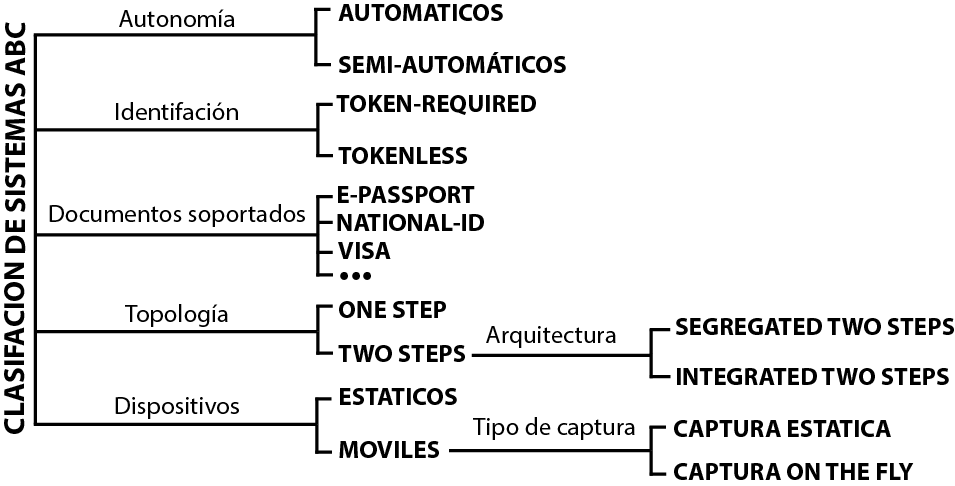
\includegraphics[width=0.8\textwidth]{ch-sistemasABC/images/ch-SistemasABC/CATERGORIAS_DE_ABCS.png}     \caption{Categorías de los sistemas \GLS{ABC} atendiendo a distintos aspectos.}
    \label{fig:categoriasABC}
\end{figure}


Los sistemas \GLS{ABC} se pueden clasificar atendiendo a distintas características (Ver Fig. \ref{fig:categoriasABC}): Atendiendo al grado de autonomía del viajero, al tipo de identificación, al tipo de documentos capaz de procesar, a su topología o atendiendo al tipo de dispositivos de adquisición.

\begin{itemize}
%%%%%%%%%%%%%%%%%% SISTEMAS ABC:POR AUTONOMIA 
\item
Tipos de \GLS{ABC} \textbf{atendiendo a su autonomía}

Los sistemas \GLS{ABC} pueden ser automáticos o semiautomáticos \footnote{Los sistemas automáticos también se conocen como desatendidos y a los semiautomáticos como atendidos.}, dependiendo de si el viajero puede realizar todos los procesos de manera automática sin requerir ningún tipo de asistencia por parte de los agentes de seguridad. (Que un agente sea requerido para subsanar una incidencia no hace que el sistema deje de ser considerado como automático).

%%%%%%%%%%%%%%%%%% SISTEMAS ABC:POR MODO DE IDENTIFICADION
\item
Tipos de \GLS{ABC} \textbf{atendiendo al modo de identificación}

Dependiendo de si el sistema requiere un \textit{\gls{token}} para identificar al viajero se distinguen dos tipos de sistemas: \textbf{\textit{\gls{token-required}}} o \textbf{\textit{\gls{tokenless}}} \cite{ISO/Biometric}.

\begin{itemize}
    \item
    \textit{\textbf{\gls{token-required}}}:
    Requieren de un \textit{\gls{token}}, para realizar la identificación del viajero, que bien puede ser un \textit{\gls{token} físico}, como el propio \gls{e-passport} u otro \gls{eMRTD}, o bien un \textbf{\textit{\gls{token}} lógico} que puede ser una \textbf{clave} o un rasgo biométrico pre-registrado\footnote{Algunas publicaciones consideran los sistemas que usan \gls{biometria} pre-registrada como \gls{tokenless}.}.
    \item
    \textit{\textbf{\gls{tokenless}}}:
    No requieren de un \textit{\gls{token}} para realizar la identificación del viajero. El viajero puede presentar un rasgo biométrico al sistema y éste realiza una búsqueda \textbf{$(1:n)$} con todos los usuarios del sistema.
\end{itemize}

Normalmente los cruces de frontera requieren que los viajeros porten algún documento identificativo por lo que la mayoría de los sistemas \GLS{ABC} instalados en cruces de frontera son \GLS{ABC} \textit{\gls{token-required}}.

%%%%%%%%%%%%%%%%%% SISTEMAS ABC:POR DOCUMENTOS QUE PROCESAN
\item
Tipos de ABC \textbf{atendiendo a los documentos que procesan}

Los sistemas \GLS{ABC} pueden clasificarse dependiendo de los documentos que puede procesar: \gls{e-passport}, \gls{nacional-ID}\footnote{Algunos países de la \GLS{EU}, como España o Alemania disponen de documentos de identificación  \gls{eID}, con información biométrica del propietario y que son válidos para el cruce de fronteras.}, \Gls{visa}\footnote{En la \GLS{EU} el documento \GLS{visa} es un documento de viaje obligatorio en para muchos países fuera del acuerdo \gls{Schengen}.}. 

%%%%%%%%%%%%%%%%%% SISTEMAS ABC:POR TOPOLOGIA
\item
Tipos de \GLS{ABC} \textbf{atendiendo a su topología}

Los sistemas \GLS{ABC} dependiendo del número de dispositivos y de los procesos que se realizan en cada uno de ellos se distinguen sistemas \GLS{ABC} \textit{<<One Step>>}, \textit{<<Integrated Two Step>>}, o \textit{<<Segregated Two Step>>}. (En las Sección \ref{subsec:Topologias} se explica en detalle cada una de las topologías). 

%%%%%%%%%%%%%%%%%% SISTEMAS ABC:POR DISPOSITIVOS DE ADQUISICION
\begin{figure}
 \centering
     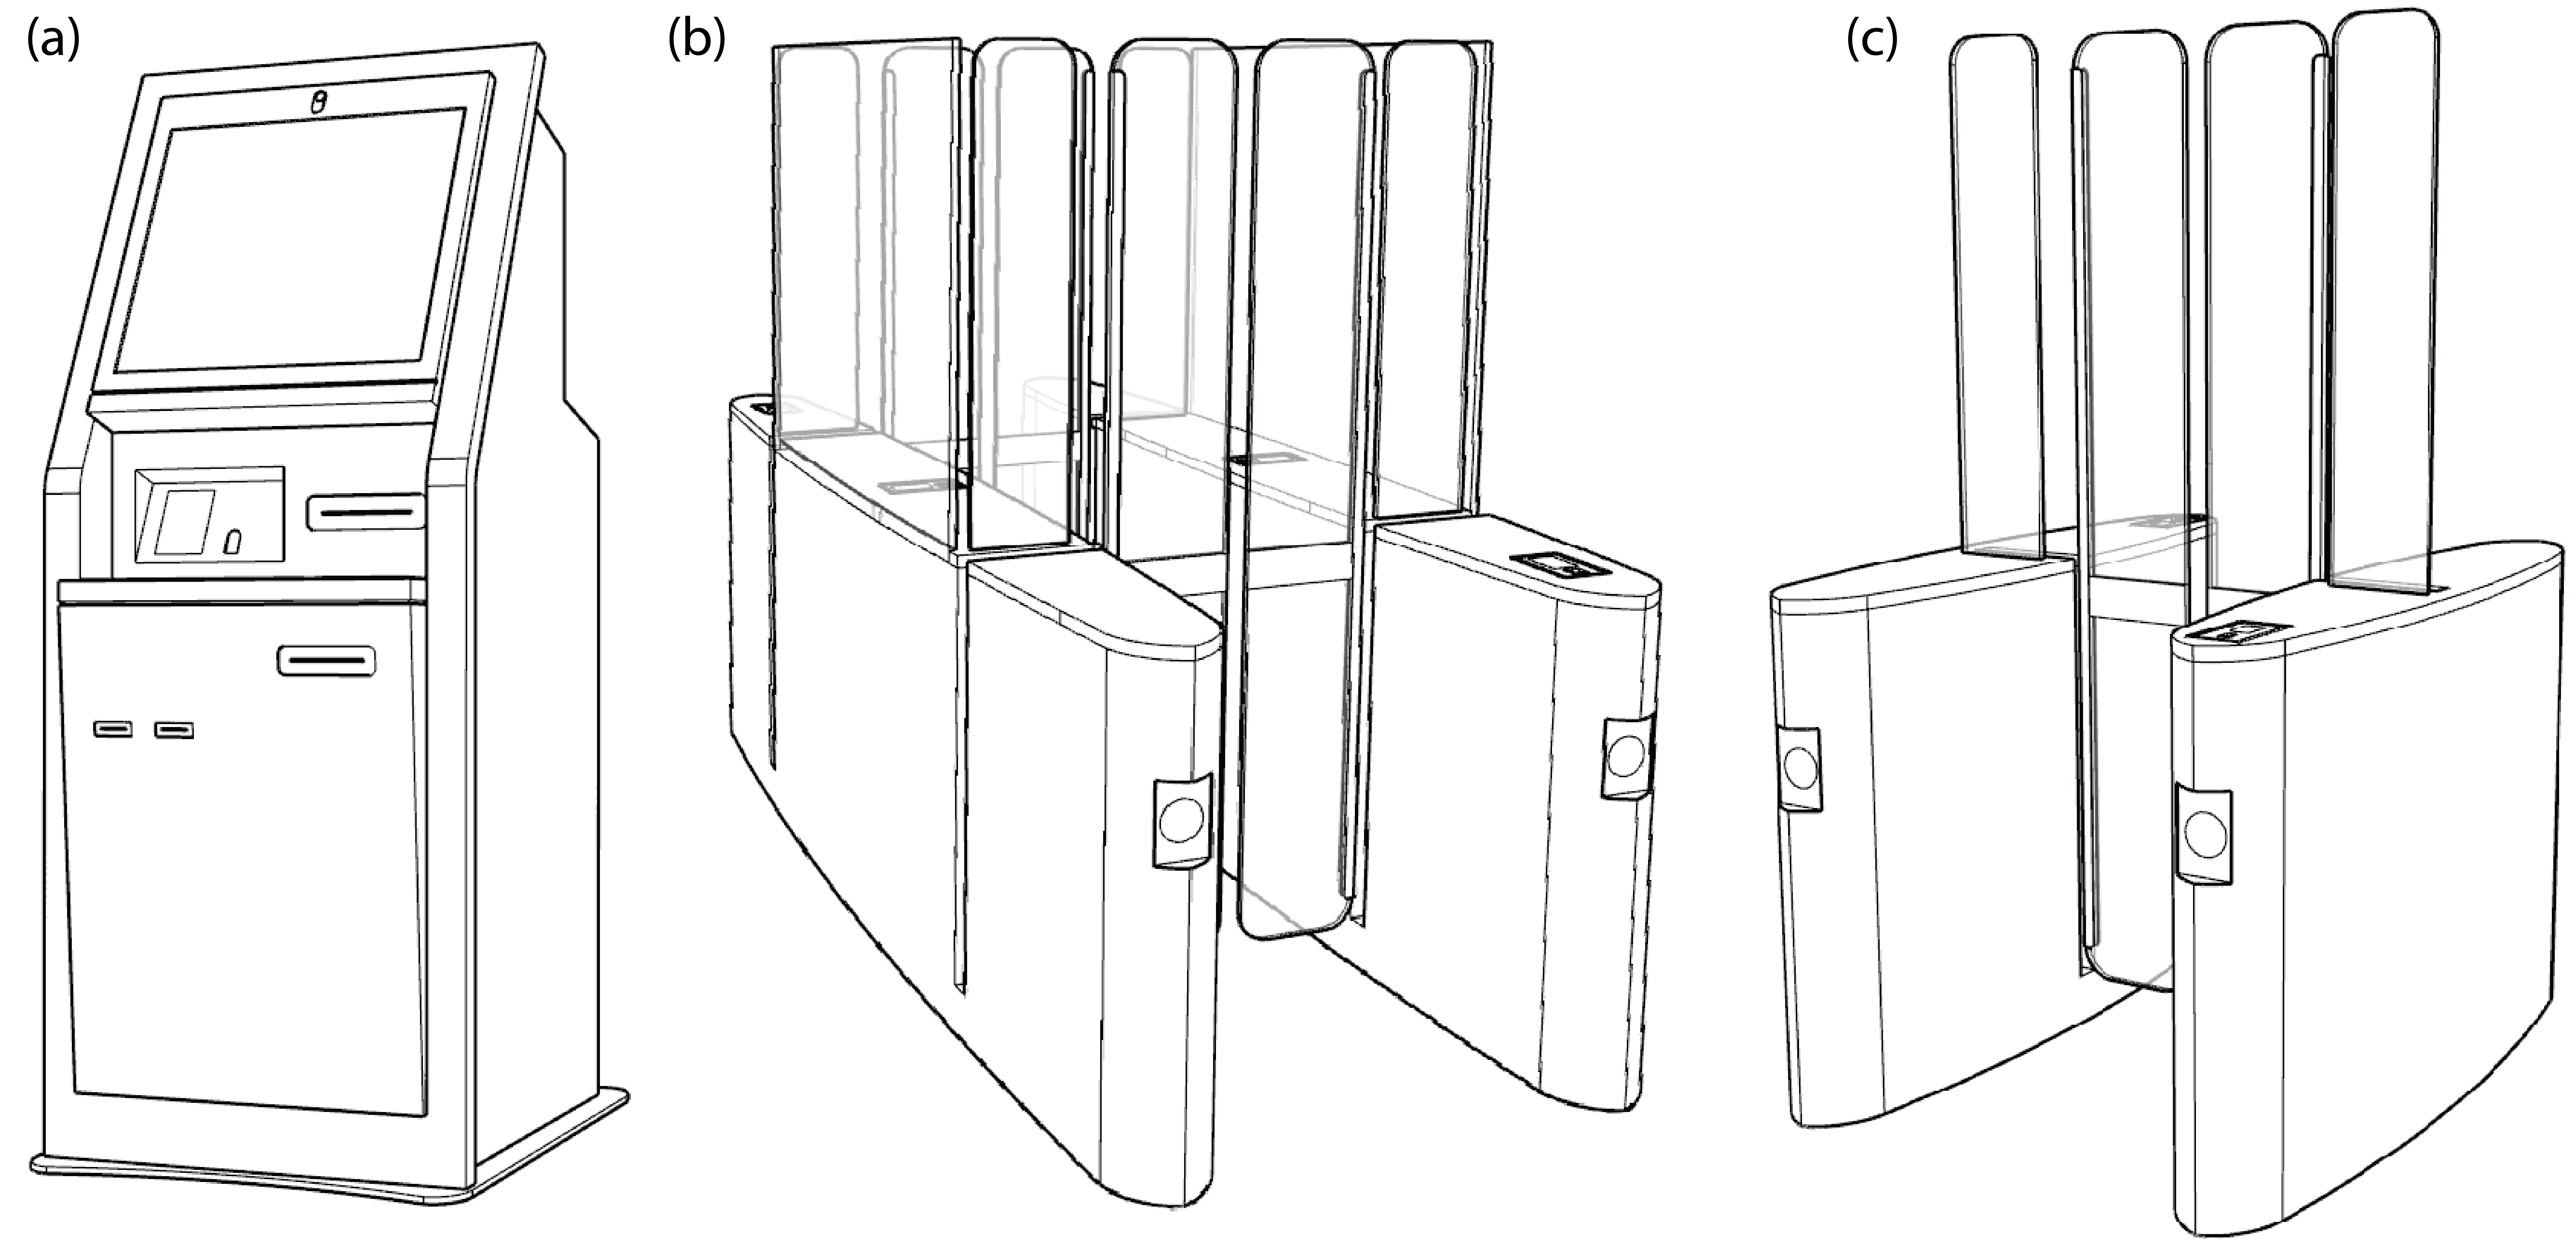
\includegraphics[width=0.8\textwidth]{ch-sistemasABC/images/ch-SistemasABC/dispositivosABCEstaticos.png}
     \caption{(a) \gls{e-kiosk}, (b) \textit{e-gate mantrap} y (c) \gls{e-gate} con una barrera.}
    \label{fig:dispositivosABCEstaticos}
\end{figure}

\item
Tipos de \GLS{ABC} \textbf{atendiendo a los dispositivos de adquisición}

Dependiendo de los dispositivos en los que se implementa el sistema, Un \GLS{ABC} puede ser: \GLS{ABC} estáticos cuando los dispositivos no pueden desplazarse (Figura \ref{fig:dispositivosABCEstaticos}) y es el viajero quien debe aproximase al dispositivos para ser identificado y \GLS{ABC} móviles, cuando el sistema se ha implementado en un dispositivos móviles (por ejemplo una \textit{tablet}) y es el agente quien se aproxima al viajero para realizar la identificación.

\medskip
\textbf{\GLS{ABC} estáticos}

Dentro de los dispositivos estáticos, se pueden distinguir un nuevo tipo sistemas que son los Sistemas \GLS{ABC} estáticos con captura \gls{OnTheFly} o sistemas \GLS{ABC} \gls{OnTheFly} (Descritos en detalle en el capitulo \ref{ch:ABC_OnTheFly}) que se diferencian de los sistemas \GLS{ABC} con captura estática en que no requieren que el viajero se detenga frente al dispositivo.  

\medskip
\textbf{\GLS{ABC} móviles}

Fronteras exteriores donde se requiere una identificación pero no es posible el uso de \glspl{e-gate}, como por ejemplo cruces de fronteras en autobuses, coches o trenes.

Los sistemas móviles son útiles también, como sistemas adicionales y de apoyo a para los agentes en las puertas \GLS{ABC}.

Los requisitos básicos a los que deben atender los sistemas \GLS{ABC} móviles son:

\begin{itemize}
\item
\Gls{captura} de datos biométricos de forma cómoda y confiable.

\item
Seguridad en las comunicaciones inalámbricas.

\item
Dispositivos móviles adaptados al trabajo de los agentes de seguridad: \Gls{usabilidad}, duración de las baterías, robustez, \textit{Human-Machine Interface} (\textbf{\GLS{HMI}}).

\end{itemize}

\end{itemize}



%%%%%%%%%%%%%%%%%%%%%%%%%%%%%%%%%%%%%%%%%%%%%%%%%%%%%%%%%%%%%%%%
%%%%  ATAQUES DE PRESENTACION %%%%%%%%%%%%%%%%%%%%%%%%%%%%%%%%%
%%%%%%%%%%%%%%%%%%%%%%%%%%%%%%%%%%%%%%%%%%%%%%%%%%%%%%%%%%%%%%%%
\section{Ataques de presentación}\label{sec:ContextoAtaquesPresentacion}

\begin{figure}[t]
    \centering
    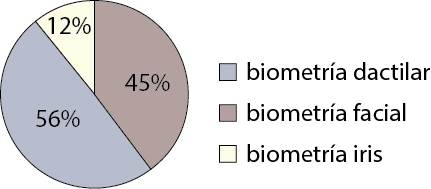
\includegraphics[width=0.6\linewidth]{ch-sistemasABC/images/ch-SistemasABC/PORCENTAJES_TIPOS_BIOMETRIAS.png}
    \caption{Porcentaje de sistemas \GLS{ABC} con distintos tipos de biometría \cite{donida2016emerging}.}
    \label{fig:ABCDisintasBiometrias}
\end{figure}

Los componentes de los sistemas \GLS{ABC} encargados de la identificación del viajero mediante sus rasgos biométricos componen un subsistema biométrico (\GLS{BVS} ver sección \ref{subsec:ArquitecturaLogicaABC}). Los rasgos más comúnmente utilizados son los recomendados por \GLS{ICAO} \cite{doc20069303}: La cara, las huellas dactilares y el \gls{iris} (ver Fig. \ref{fig:ABCDisintasBiometrias}). Sin embargo también hay sistemas que usan rasgos biométricos diferentes o que emplean técnicas de multi-biometría (ver Apéndice \ref{apendix:Biometria}).

%%%%%%%%%%%%%%%%%%% SEGURIDAD_BIOMETRICOS:ATAQUES DE PRESENTACION %%%%%%%%%%%%%%%%%%%%%%%%%%%%%%%%%%%%%%%%%
\subsection{Ataques de presentación: PA}\label{subsec:AtaquesPresentacion}

El subsistema \GLS{BVS} puede ser atacado en distintos puntos (para más detalles sobre ataques a un sistema biométrico ver Apéndice \ref{apendix:Biometria}), pero uno de los ataques más comunes, ya que no requiere de altos conocimientos técnicos de la implementación del sistema, son los ataques de presentación, \textit{Presentation Attack} (\GLS{PA}) que se producen en la adquisición del rasgo biométrico, a nivel del sensor.

Los ataques de presentación tienen como objetivo interferir el sistema de forma que no pueda diferenciar entre el ataque y la presentación del rasgo biométrico real (\gls{bona-fide}) para suplantar otra identidad o para no ser reconocido, por lo que dentro de los sujetos que realizan estos ataques se pueden distinguir dos tipos:

\begin{itemize}
    \item 
    El impostor, que intenta ser reconocido por el sistema como otro individuo, suplantando la identidad de un usuario del sistema.
    
    El impostor a su vez puede tratar de hacerse pasar por un usuario especifico del sistema o bien puede ser que trate de hacerse pasar por un usuario valido para el sistema sin importar por cual. 
    
    \item 
    El ocultador, que intenta no ser reconocido por el sistema. Oculta o altera sus propias características biométricas para no ser detectado como un usuario que el sistema conoce.
\end{itemize}

Es relativamente fácil conseguir rasgos biométricos para construir un artefacto, con o sin el consentimiento del propietario, ya que existe poca concienciación de que las información biométrica debe protegerse. No es difícil robar un rasgo biométrico: Huellas dactilares a partir de una huella latente o artefactos para suplantar una cara con las imágenes compartidas en las redes sociales \cite{xu2016virtual}.

Este tipo de ataques pueden realizarse mediante muchos medios: artefactos, mutilaciones, replicas, etc. y cada vez son más sofisticados por la aparición de nuevos mecanismos y nuevos materiales.

Dentro de los ataques de presentación se consideran distintas estrategias.

\textbf{Falso registro}

Cuando se usa un documento falsificado o manipulado. 

\textbf{Falsa biometría física}

Usar una característica biométrica sintética (o artefacto) para engañar al sistema.

\textbf{Falsa biometría digital}

Reutilización de residuos biométricos 

\textbf{Maquillaje}

 Muchos artistas del maquillaje presentan en internet tutórales que permiten replicar en una cara las características de otra cara. El maquillaje radical o \textit{contouring} borra los rasgos de un rostro y replica exactamente los rasgos de otro \ref{fig:Maquillajes}, permitiendo engañar a los sistemas de reconocimiento \gls{facial}.  

\textbf{Mascaras}

Uso de máscaras hiperrealistas, difíciles de detectar en una inspección visual, para suplantar la identidad de otro individuo. Estas mascaras ya se han usado para cometer otros delitos (ver Fig. \ref{fig:DelitosConMascaras}).

% \color{red}
% Detectable en algunas zonas donde no hay mascara, boca, ojos, etc.
% Este tipo de máscaras no reproducen correctamente los rasgos juveniles.

% El uso de biometría multimodal puede dificultar la suplantación de identidad, al obligar al atacante a tener más inflación sobre el usuario legitimo. pero este tipo de biometría requiere algún método de fusión para los resultados obtenidos para cada biometría.

% En los sistemas \GLS{ABC} cuando se produce un ataque de suplantación es aconsejable que una alarma interna avise a los agentes que monitorizan el sistema y no, alertar al viajero, que posiblemente sea un atacante. 
% \color{black}


%%%%%%%%%%%%%%%%%%%%%%%%%%%%%%%%%%% SEGURIDAD_BIOMETRICOS:TIPOS DE ATAQUES DE PRESENTACION %%%%%%%%%%%%%%%%%%%%%%%%%%%%%%%%%%% 
\subsection{Tipos de ataques presentación: PAI}\label{sec:PAI}

\color{red} gráfico con los tipos de PAI\color{black}

Los ataques de presentación pueden clasificarse atendiendo al objeto o al instrumento utilizado para realizar el ataque. Estos objetos se conocen como \Glspl{PAI} (ver Fig. \color{red}tabla con los PAI\color{black}). Un \GLS{PAI} es una reproducción de un rasgo biométrico, un artefacto u otro tipo de objeto empleado para realizar los ataques de presentación. Un \GLS{PAI} puede ser un artefacto, pero también puede ser un rasgo biométrico amputado de un cadáver o un rasgo biométrico alterado del propio impostor. Las características que debe tener un \GLS{PAI} para poder engañar al sistema son:

\begin{itemize}
\item
Debe poder ser adquirido por el sensor, si no puede ser adquirido, el sistema directamente lo considerará un ataque. Por ejemplo las huellas de silicona que no son legibles por un lector capacitivo de huellas dactilares.

\item
Debe tener la suficiente calidad como por que sea posible extraer las características requeridas por el sistema biométrico.

\item
Calidad suficiente para obtener un buen \textit{score} de reconocimiento en el sistema biométrico.

\item
Debe ser lo suficientemente discreto para no ser detectado por un operador que esté monitorizando el sistema en el caso de que sea atendido o semi-atendido. 
\end{itemize}


\begin{figure}[t]
    \centering
    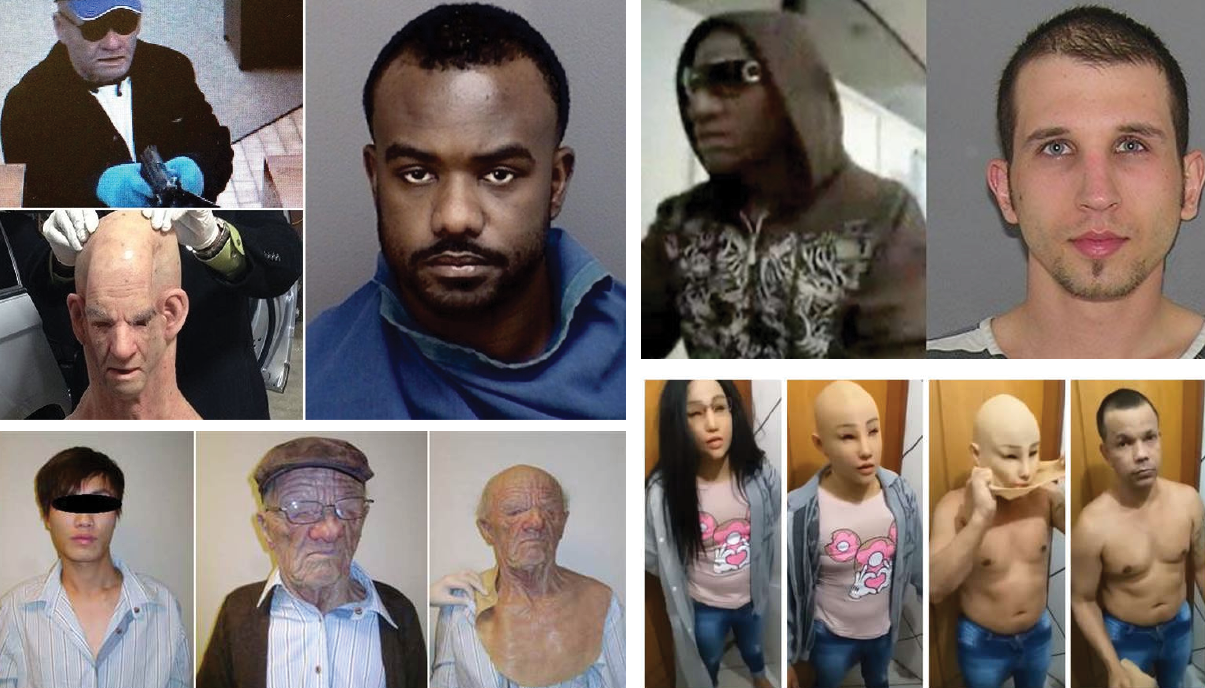
\includegraphics[width=0.8\linewidth]{ch-sistemasABC/images/ch-SistemasABC/DELITOS_CON_MASCARAS.png}
    \caption{Delincuentes haciendo uso de máscaras hiperrealistas de Látex.}
    \label{fig:DelitosConMascaras}
\end{figure}


\begin{figure}[t]
    \centering
    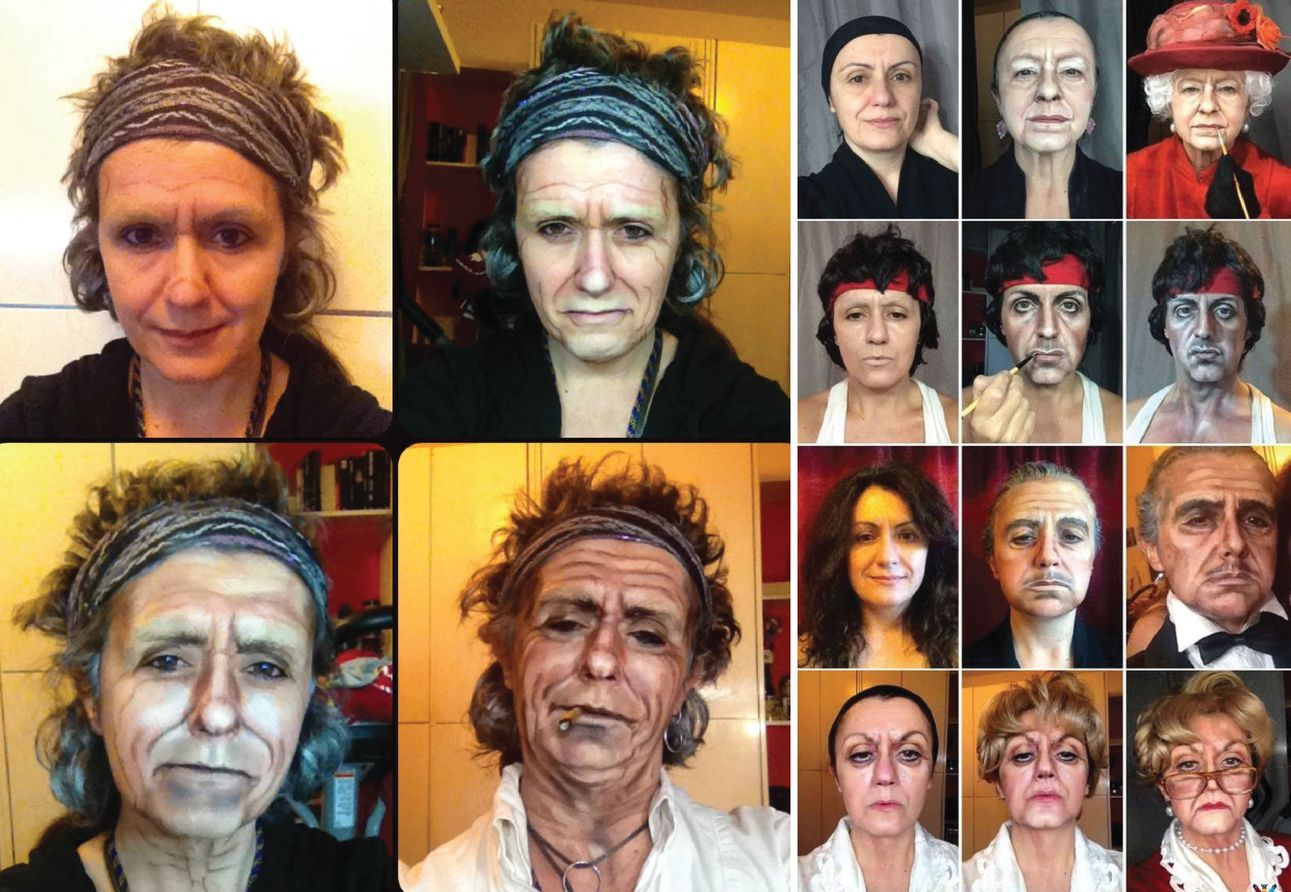
\includegraphics[width=0.8\linewidth]{ch-sistemasABC/images/ch-SistemasABC/MAQUILLADORA_LUCIA_PITTALIS.png}
    \caption{Trabajos de la maquilladora Lucia Pittalis \cite{LuciaPittalisOnline}.}
    \label{fig:Maquillajes}
\end{figure}


Es fácil encontrar distribuidores de mascaras, prótesis y pelucas hiperrealistas que replican perfectamente los rasgos de una persona mediante fotografías (SPFXmask \cite{spfxmaskOnline}, HyperFlesh\cite{HyperFleshOnline}, RealFleshMask \cite{RealFleshMaskhOnline}, ThatsMyFace \cite{ThatsMyFaceOnline}) (ver Fig. \ref{fig:DelitosConMascaras})).

%%%%%%%%%%%%%%%%%%%%%%%%%%%%%%%%%%%  SEGURIDAD_BIOMETRICOS:DETECCION DE ATAQUES DE PRESENTACION %%%%%%%%%%%%%%%%%%%%%%%%%%%%%%%%%%% 
\subsection{Detección de ataques de presentación: PAD}\label{sec:PAD}

Usar biometría en sistemas no supervisados conlleva más riesgos que en sistemas supervisados. Un sistema completamente automático puede ser atacado más fácilmente que uno semiautomático donde alguien controla la adquisición del rasgo biométrico para la identificación. Los \textit{Presentation Attack Detection} (\GLS{PAD}) son las técnicas para detectar automáticamente los ataques de presentación en el momento de la adquisición de las características biométricas del individuo \footnote{\GLS{ISO}/\GLS{IEC} $30107$ describe en detalle muchos de estos métodos de \GLS{PAD} \cite{ISO/PADFramework}.}. Los \GLS{PAD} mitigan los riesgos de ataque y mejoran la seguridad de los sistemas biométricos no supervisados y ayudan en el control en los supervisados.

Es conveniente considerar el \GLS{PAD} como un proceso independiente a la autenticación biométrica y puede realizarse antes o después de ésta. En el mismo dispositivo en el que se realiza la adquisición o bien, mandar los datos capturados o las características a un sistema central. 

Los pasos comunes que deben seguir los métodos de \GLS{PAD} son:

\begin{itemize}
    \item
    Capturar la información biométrica del usuario mediante el sensor o sensores. Estos sensores no tienen por que ser los mismos que los empleados para la adquisición del sistema biométrico, pero es recomendable que la adquisición del \GLS{PAD} se realice de manera simultanea a la del sistema biométrico, con el fin de minimizar los riesgos de seguridad.
    
    \item
    Extracción de las características necesarias para el método \GLS{PAD} especifico. 
    
    \item
    Analizar las características dependiendo del \GLS{PAD} elegido. No hay un método \GLS{PAD} para cada tipo de \GLS{PAI}, un mismo \GLS{PAD} puede detectar distintos tipos de \GLS{PAI}.Y tampoco tiene por que ser el mismo para todos los usuarios, es posible que algunos usuarios requieran un control mas exhaustivo que otros. 
\end{itemize}


%%%%%%%%%%%%%%%%%%%%%%%%%%%%%%%%%%% SEGURIDAD_BIOMETRICOS:TIPOS DE PAD %%%%%%%%%%%%%%%%%%%%%%%%%%%%%%%%%%% 
\subsection{Tipos de PAD}\label{sec:TiposPAD}

Los métodos de \GLS{PAD} pueden ser \textit{hardware} o \textit{software} y dependiendo del nivel del sistema biométrico en el que se implementa el método se puede distinguir entre \GLS{PAD} a nivel sensor o \GLS{PAD} a nivel operacional.

Se pueden clasificar dependiendo de la estrategia que emplean para detectar el ataque.

\paragraph{PAD a nivel sensor:}
\begin{itemize}
    \item 
    \textbf{Detección de artefactos}: Detectan si la presentación está siendo realizada con un objeto sintético.
    
    Ejemplos: Detectar la conductividad de la piel con sensores capacitivos.
    \item 
    \textbf{Detección de vida} \textit{\Gls{liveness detection}}: Son métodos que evalúan las características, o \gls{liveness}, para determinar si realmente hay un individuo con vida frente al dispositivo de adquisición
    
    \Gls{liveness} es la cualidad de vida y se usa en algunos sistemas biométricos para evitar ataques con artefactos o con miembros amputados\footnote{La policía usó el dedo de un cadáver para intentar acceder a su teléfono: \href{https://www.tampabay.com/news/publicsafety/Cops-used-dead-man-s-finger-in-attempt-to-access-his-phone-It-s-legal-but-is-it-okay-\_167262017/}{https://www.tampabay.com/news/publicsafety/Cops-used-dead-man-s-finger-in-attempt-to-access-his-phone-It-s-legal-but-is-it-okay-\_167262017/}} \GLS{PAD} \cite{bhattacharjee2018spoofing} comprueban que el rasgo biométrico se está adquiriendo de una persona viva. Por ejemplos mediante la medición de la temperatura corporal, la detección de los vasos sanguíneos o el parpadeo de los ojos.
    
    Para analizar las reacciones no es suficiente una captura estática se requiere una captura que dure un periodo de tiempo suficiente para que tenga lugar la reacción.
    
    Se pueden considerar $3$ tipos de indicadores que se usan para confirmar una presentación con vida.

    \begin{itemize}
      \item 
      \textbf{Características físicas o anatómicas}: Adsorción de la luz por la piel. Transmisión de electricidad por el cuerpo humano. Transpiración de los dedos. Movimientos del \GLS{iris} o parpadeos. Detección del pulso. Flujo sanguíneo.
      \item
      \textbf{Reacciones involuntarias}: Pulso o dilatación del la pupila al recibir una luz potente.
      \item
      \textbf{Reacciones voluntarias}: Elegir un dedo de la mano. Guiñar un ojo o colocar la mano de una manera determinada.
    \end{itemize}
    
    Algunos métodos para la detección de vida usan estrategias similares a las de reto-respuesta.
    
    \item 
    \textbf{Detección de alteraciones}: Detectar las alteraciones o ocultaciones de un rasgo biométrico.
    
    Ejemplo: Ocultar las huellas dactilares mediante cicatrices. Lentillas sintéticas.
    \item 
    \textbf{Detección de no conformidad}: Detecta conductas extrañas en el usuario al realizar la presentación. 
    
    Ejemplo: No tomar la pose adecuada para la captura \gls{facial} o intentar colocar mal el dedo en el escáner \gls{dactilar}.
    \item 
    \textbf{Detección de coacción}: Detectar si el usuario está siendo coaccionado para realizar realizar la presentación. 
    
    Ejemplos: Detecta rasgos faciales de emociones como el miedo, la angustia, el nerviosismo o el estrés. 
    \item 
    \textbf{Detección de oclusión}: Detecta si el rasgo biométrico o el sensor está siendo ocluido parcial o totalmente. 
    
    Ejemplo: Detectar si el usuario lleva algún complemento que pueda ocluir la captura: Gafas de sol, bufandas, sobreros o guantes. Detectar si algo esta tapando la cámara o el escáner dactilar.
\end{itemize}
    
\paragraph{PAD a nivel operacional:}
\begin{itemize}
    \item 
    \textbf{Limitación de fallos de adquisición}: Contabilizar el número de fallos de adquisición y si se supera un determinado número de fallos la la presentación, considerar lar presentación como un ataque.
    \item
    \textbf{Circunstancias no habituales}: Si la localización o el momento en el que se produce la presentación no es un lugar o un horario habitual, se puede considerar la presentación como un ataque o al menos lanzar una alerta al sistema.  
    \item
    \textbf{Reto-respuesta} (\textit{\gls{challenge response}}): Estrategia que se usa para la autenticación de usuarios que consiste en plantear un reto que requiere una determinada actuación razonada por parte del usuario \cite{shoukry2015pycra}. Normalmente se usa para la autenticación en sistemas no exclusivamente biométricos, donde al usuario se le hace una pregunta o directamente se le solicita una clave.
    
    En los sistemas biométricos la estrategia reto-respuesta se usa como \GLS{PAD} de detección de vida y que los retos plateados pueden ser voluntarios (detección de vida <<activa>>) o involuntarios (detección de vida <<pasiva>>).
    
    \begin{itemize}
        \item
        \textbf{Involuntario}: 
        Un estimulo que provoque una acción determinada, una luz fuerte que provoque una dilatación de la pupila o parpadeos en el usuario \cite{rigas2015eye}.
        \item
        \textbf{Voluntario}:
        Hacer que el usuario dirija su mirada a una determinada región de la pantalla, que guiñe un ojo o que presente al sensor un dedo determinado u otro.
    \end{itemize} 
\end{itemize}

%%%%%%%%%%%%%%%%%%%%%%% ATAQUES DE PRESENTACION Y PAD EN ABC %%%%%%%%%%%%%%%%%%%%%%
\subsection{Ataques de presentación y PAD en sistemas ABC}\label{subsec:PA-biometriasABC}

%%%%%%%%%%%%%%%%%%%%%%% ATAQUES DE PRESENTACION  BIOMETRIA FACIAL %%%%%%%%%%%%%%%%%%%%%%
\paragraph{Ataques de presentación en la biometría facial}
Los ataques de suplantación el la \gls{biometria} \gls{facial} de los sistemas \GLS{ABC} puede producirse de forma directa, mediante un \GLS{PAI} que reproduzca los rasgos faciales del viajero suplantado (Máscaras, maquillaje, etc.) o de forma indirecta, alterando la información biométricas almacenada en el chip del \gls{eMRTD} (\Gls{morphing}).

Los ataques directos pueden ser más o menos detectables por parte de los agentes que monitorizan el sistema. Por ejemplo, una fotografía del viajero o un dispositivos que reproduzca su imagen, pueden engañar al sistema biométrico, pero difícilmente pasarán desapercibidos a los agentes de frontera. Sin embargo, otros \GLS{PAI} como una mascara o prótesis de silicona, o un buen maquillaje  pueden engañar al sistema biométrico y también pueden ser \textbf{indetectables} para los agentes (ver Fig. \ref{fig:DelitosConMascaras}).    


%%%%%%%%%%%%%%%%%%%%%%% ATAQUES DE PRESENTACION BIOMETRIA DACTILAR %%%%%%%%%%%%%%%%%%%%%%
\paragraph{Ataques de presentación en la biometría \gls{dactilar}}
Los ataques a este tipo de biométrica suelen ser \textbf{más discretos} y menos detectables para los agentes de frontera.

Para engañar a los sistemas biométricos dactilares suele usarse como \GLS{PAI} huellas impresas en papel, huellas sintéticas de látex o de gelatina colocadas sobre las huellas reales o incluso dedos amputados del viajero a suplantar. 

Para hacer frente a este tipo de ataques se pueden usar \textbf{métodos \textit{hardware}} con sensores que detectan algunos de estos \GLS{PAI} o \textbf{métodos \textit{software}} que procesan la imagen de la huella dactilar.  

Si se usan \textit{varias huellas} para la identificación, será más difícil atacar al sistema ya que el atacante necesita disponer de más información del viajero a suplantar. Además se puede hacer un control activo de \gls{liveness} solicitando aleatoriamente en la adquisición, una huella u otra.

Detectar el flujo sanguíneo mediante el análisis de las pulsaciones o mediante el análisis de los capilares venosos de la yema de los dedos.

Analizar las condiciones de la piel como la sudoración o el tamaño de algunos rasgos de la huella como los poros

%%%%%%%%%%%%%%%%%%%%%%% ATAQUES DE PRESENTACION BIOMETRIA IRIS %%%%%%%%%%%%%%%%%%%%%%
\paragraph{Ataques de presentación en la biometría del iris}
Suelen usarse lentillas con imágenes del iris del viajero a suplantar o con fotografías de alta resolución.

Para evitar estos ataques es posible analizar las micro-texturas del iris presentado o aplicar métodos de \gls{liveness} como detectar el parpadeo y de \textit{\gls{challenge response}} mediante una luz fuerte que dilate la pupila o haga parpadear al viajero.


%%%%%%%%%%%%%%%%%%%%%%%%%%%%%%%%%%% SEGURIDAD_BIOMETRICOS:EVALUACION DE LOS PAD %%%%%%%%%%%%%%%%%%%%%%%%%%%%%%%%%%% 
\subsection{Evaluación y métricas PAD}\label{sec:MetricasEvaluacionPAD}

Los \GLS{PAD} están sujetos a errores similares a los sistemas biométricos (para más información sobre las métricas de los sistemas biométricos ver Apéndice \ref{apendix:Biometria}), pero por ejemplo \Gls{FAR} no es un buen indicador para medir la vulnerabilidad de un sistema biométrico, ya que informa de cuando un usuario es aceptado como si se tratase de otro pero se esto requiere cero esfuerzo por parte del usuario que sólo hace uso de si propia biometría sin intenciones delictivas.

A partir de $2017$ (\textbf{ISO/IEC $2382$-$37$:$2017$} \cite{ISO/PADEvaluation}), se define una métrica especifica para evaluar la calidad de los sistemas \GLS{PAD}, basada en dos ratios: la tasa de los ataques clasificados de forma errónea, \textit{Attack Presentation Classificacion Error Rate} (\gls{APCER}) y la tasa de las presentaciones del rasgo real \gls{bona-fide} mal clasificadas, \textit{Bona-Fide Presentation Classification Error Rate} (\gls{BPCER}).

\GLS{APCER} y \GLS{BPCER} vienen definidas por las ecuaciones \eqref{eqn:APCER} y \eqref{eqn:BPCER}:

\begin{equation}
APCER_{PAIS} = 1 - \left( \frac{1}{N_{PAIS}} \right)\sum_{i=1}^{N_{PAIS}} \left( RES_{i} \right),
\label{eqn:APCER}
\end{equation}

donde $N_{PAIS}$ es el número de presentaciones de ataque realizados con un determinado \GLS{PAI} (dado que los ataques pueden ser muy diversos, se pueden agrupar según su \GLS{PAI}) y $RES_{i}$ toma el valor $1$ si la presentación \textit{i} es clasificada como ataque y $0$ si es clasificada como \gls{bona-fide}.  

\begin{equation}
BPCER_{PAIS}=\frac{\sum_{i=1}^{N_{BF}} RES_{i}} {N_{BF}},
\label{eqn:BPCER}
\end{equation}

donde $N_{BF}$ es el número de presentaciones \gls{bona-fide} y $RES_{i}$ toma el valor $1$ si la presentación \textit{i} es clasificada como ataque y $0$ si es clasificada como \gls{bona-fide}.  

Habitualmente la respuesta de un sistema \GLS{PAD} es una probabilidad, lo que hace que los valores \GLS{APCER} y \GLS{BPCER} dependan de un umbral con el que se decide si la presentación es un ataque o un \gls{bona-fide}, si la probabilidad es menor o mayor al umbral. 


\begin{figure}
    \centering
    \includegraphics[width=0.8\textwidth]{ch-sistemasABC/images/ch-SistemasABC/EJEMPLO_CURVA_DET_APCER_BPCER.png}
    \caption{Ejemplo de curva \GLS{DET} con el \GLS{APCER} y el \GLS{BPCER} de dos \GLS{PAD}, donde PAD-B es más vulnerable que PAD-A.}
    \label{fig:ejemploCurvaAPCER-BPCER}
\end{figure}

% \begin{SCfigure}[]
%     \centering
%     \sidecaptionvpos{figure}{t}
%     \caption{Ejemplo de curva \GlS{DET} con el \GlS{APCER} y el \GSL{BPCER} de dos \GSL{PAD}, donde PAD-B es más vulnerable que PAD-A.}
%     \includegraphics[width=0.5\textwidth]{ch-sistemasABC/images/EJEMPLO_CURVA_DET_APCER_BPCER.png}
%     \label{fig:ejemploCurvaAPCER-BPCER}
% \end{SCfigure}

Trazando una curva \textit{Error Trade-Off} (\GLS{DET}) con los valores \GLS{APCER} y \GLS{BPCER} para los distintos umbrales es posible visualizar el rendimiento del sistema \GLS{PAD} y comparar unos sistemas con otros. Las curvas más cercanas al origen presentan un \GLS{D-EER} más bajo y por lo tanto un mejor rendimiento (ver Fig. \ref{fig:ejemploCurvaAPCER-BPCER}). 

Al igual que en los sistemas biométricos, ambas tasas, \GLS{APCER} y \GLS{BPCER}, no pueden ser minimizados. \GLS{APCER} se considera una medida de la seguridad del sistema, mientras que el \GLS{BPCER} es una medida de la conveniencia del sistema y normalmente la disminución del \GLS{APCER} implica un aumento del \GLS{BPCER}. En los sistemas \GLS{ABC} debe considerarse la seguridad como el factor más importante frente a la conveniencia. Es aconsejable establecer un valor umbral que devuelva un bajo \GLS{APCER} aunque aumente el \GLS{BPCER}. Ya que los sistemas \GLS{ABC} deben estar controlados por un agente, siempre que una presentación \gls{bona-fide} sea considerada como un ataque, disparará una alarma, que puede ser verificada y corregida por un agente

Otra manera de mostrar el rendimiento de un sistemas \GLS{PAD} consiste en presentar el porcentaje de \gls{bona-fide} mal clasificados (\GLS{BPCER}) cuando se fija un porcentaje de ataques clasificados erróneamente (\GLS{APCER}). (p. ej. Porcentaje de \GLS{BPCER} cuando el \GLS{APCER} es un $5$\%).

Una buena forma de determinar un umbral de aceptación es elegir el umbral en el que los valores de \GLS{BPCER} y \GLS{APCER} son iguales. Este valor se conoce \textit{Detection Equal Error Rate} (\GLS{D-EER}) (ver Fig. \ref{fig:ejemploCurvaAPCER-BPCER}).

.


%ESTO ES DEL PAPER DE MORHPING SE PUEDE BORRAR SI NO APORTA MAS DE LO QUE HAY METIDO
% This section presents the evaluation metrics commonly followed in the morphing attacks detection approaches and the results obtained in the presented work.

% \subsection{Evaluation metrics}\label{sec:EvaluationMetrics}

% Recently, the community has achieved a common standard ISO (IEC 30107-3:2016) \cite{ISO/PADEvaluation} to evaluate PAD systems. In this standard, the capability of the attack detection is measured with the following errors: attack presentation classification error rate (APCER) and bona fide presentation classification error rate (BPCER). This measure can be defined as follows:

% \begin{itemize}
%     \item \textbf{Attack presentation classification error rate (APCER)} is defined as the proportion of presentation attacks that have been classified incorrectly (as bona fide) \cite{ISO/PADEvaluation} (Equation \ref{eqn:APCER}).
%     \item \textbf{Bona fide presentation classification error rate (BPCER)}  is defined as the proportion of bona fide presentation incorrectly classified as presentation attacks \cite{ISO/PADEvaluation} (Equation \ref{eqn:BPCER}).
% \end{itemize}

% \begin{equation}
% APCER_{PAIs} = 1 - \left( \frac{1}{|PAI|} \right)\sum_{\omega=1}^{|PAI|} \left( RES_{\omega} \right),
% \label{eqn:APCER}
% \end{equation}

% where $|PAI|$ is the number of presentation attack instruments (PAI) and $RES_{\omega}$ takes the value $1$ if the presentation $\omega$ is assessed as attack and $0$ if it is evaluated as bona fide. A PAI is defined as a used object or biometric trait in a presentation attack.

% \begin{equation}
% BPCER_{PAIs}=\frac{\sum_{\omega=1}^{|BF|} RES_{\omega}} {|BF|},
% \label{eqn:BPCER}
% \end{equation}

% where $|BF|$ is the cardinality of bona fide presentations and $RES_{i}$ returns the value $1$ if the presentation \textit{$\omega$} is allocated as an attack and $0$ if it is analyzed as bona fide. 

% An APCER-BPCER DET curve (detection error trade-off) and the EER (equal error rate) where both errors are identical, provides a comparison among MAD systems.


%%%%%%%%%%%% BASES DE DATOS %%%%%%%%%%%%%%%%%%%%%
\chapter{Bases de datos}\label{ch:BBDDs}

\begin{table}[ht!]
     \centering
     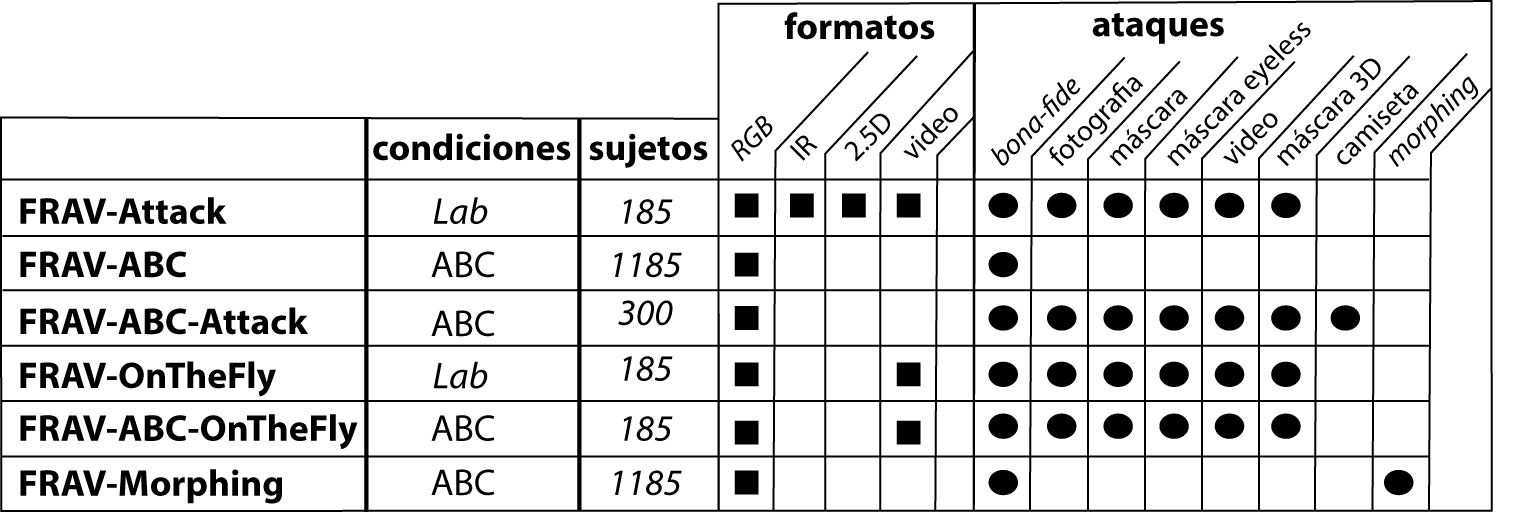
\includegraphics[width=1\textwidth]{ch-sistemasABC/images/ch-BBDDs/TABLA_BASES_DE_DATOS.png}
     \caption{Bases de datos para la detección de ataques de presentación en sistemas \GLS{ABC}.}
     \label{tab:TablaBasesDatos}
\end{table}

En cada una de las secciones de este capítulo se describen las características de las bases de datos construidas para llevar a cabo las investigaciones expuestas a lo largo de los siguientes capítulos. En la tabla \ref{tab:TablaBasesDatos} se pueden ver algunas características de cada una de estas bases de datos: número de sujetos, ataques de presentación considerados y dispositivo o dispositivos empleados para su captura.

En la sección \ref{sec:BBDD-FRAV-Attack} se presenta \Gls{FRAV-Attack}, una base de datos con ataques de presentación llevados a cabo con distintos artefactos y capturados con diferentes tipos de sensores. Con esta base de datos, capturada en laboratorio, se ha entrenamiento el método \GLS{PAD} descrito en el capitulo \ref{ch:PAD_MULTIATAQUE} y que se puso a prueba en condiciones reales en los experimentos descritos en el capitulo \ref{ch:EVALUACIONACION_TOPOLOGIAS}. 


A continuación, en la sección \ref{sec:BBDD-ABC} se presentan dos bases de datos capturadas en dispositivos \GLS{ABC} operativos, en cruces de frontera reales: \Gls{FRAV-ABC} con imágenes \textit{<<\gls{chip}>>} de pasaportes e imágenes \gls{vivo} capturadas en el propio dispositivo y \Gls{FRAV-ABC-Attack} con los mimos tipos de imágenes pero que además incluye ataques de presentación en las imágenes \gls{vivo}.

En la sección \ref{sec:BBDD-OnTheFly} se describen otras dos bases de datos construidas para el la publicación \cite{ortega2020dynamic}, que se detalla en el capítulo \ref{fig:EsquemaCapturaFRAVABCOmTheFly}. Por un lado la base de datos \Gls{FRAV-OnTheFly} capturada en un laboratorio, en condiciones controladas, simulando el comportamiento de viajeros frente a un sistema \GLS{ABC} con captura dinámica (para mas información sobre este tipo de sistemas \GLS{ABC}. ver apartado \ref{subsec:ArquitecturaFisicaABC}). Y por otro lado, las base de datos \Gls{FRAV-ABC-OnTheFly}, capturada en \GLS{ABC} con captura dinámica, en un cruce de fronteras real.

La sección \ref{sec:BBDD_Morphing} describe la base de datos, \gls{FRAV-Morphing}, construida a partir de \GLS{FRAV-ABC} para la investigación publicada sobre ataques de \gls{morphing} en sistemas \GLS{ABC} \cite{ortega2020border} que se presenta en detalle en el capitulo \ref{ch:morphing}. Además de describir la estructura de la base de datos también se detalla cómo se construyeron las imágenes con los ataques \gls{morphing}.


%%%%%%%%%%%%%% FRAV ATTACK    %%%%%%%%%%%%%%%%%%%%%%%%%%%%%%
\section{FRAV-Attack: Base de datos multimodal de ataques biométricos}\label{sec:BBDD-FRAV-Attack}

\begin{figure}[t!]
\centering
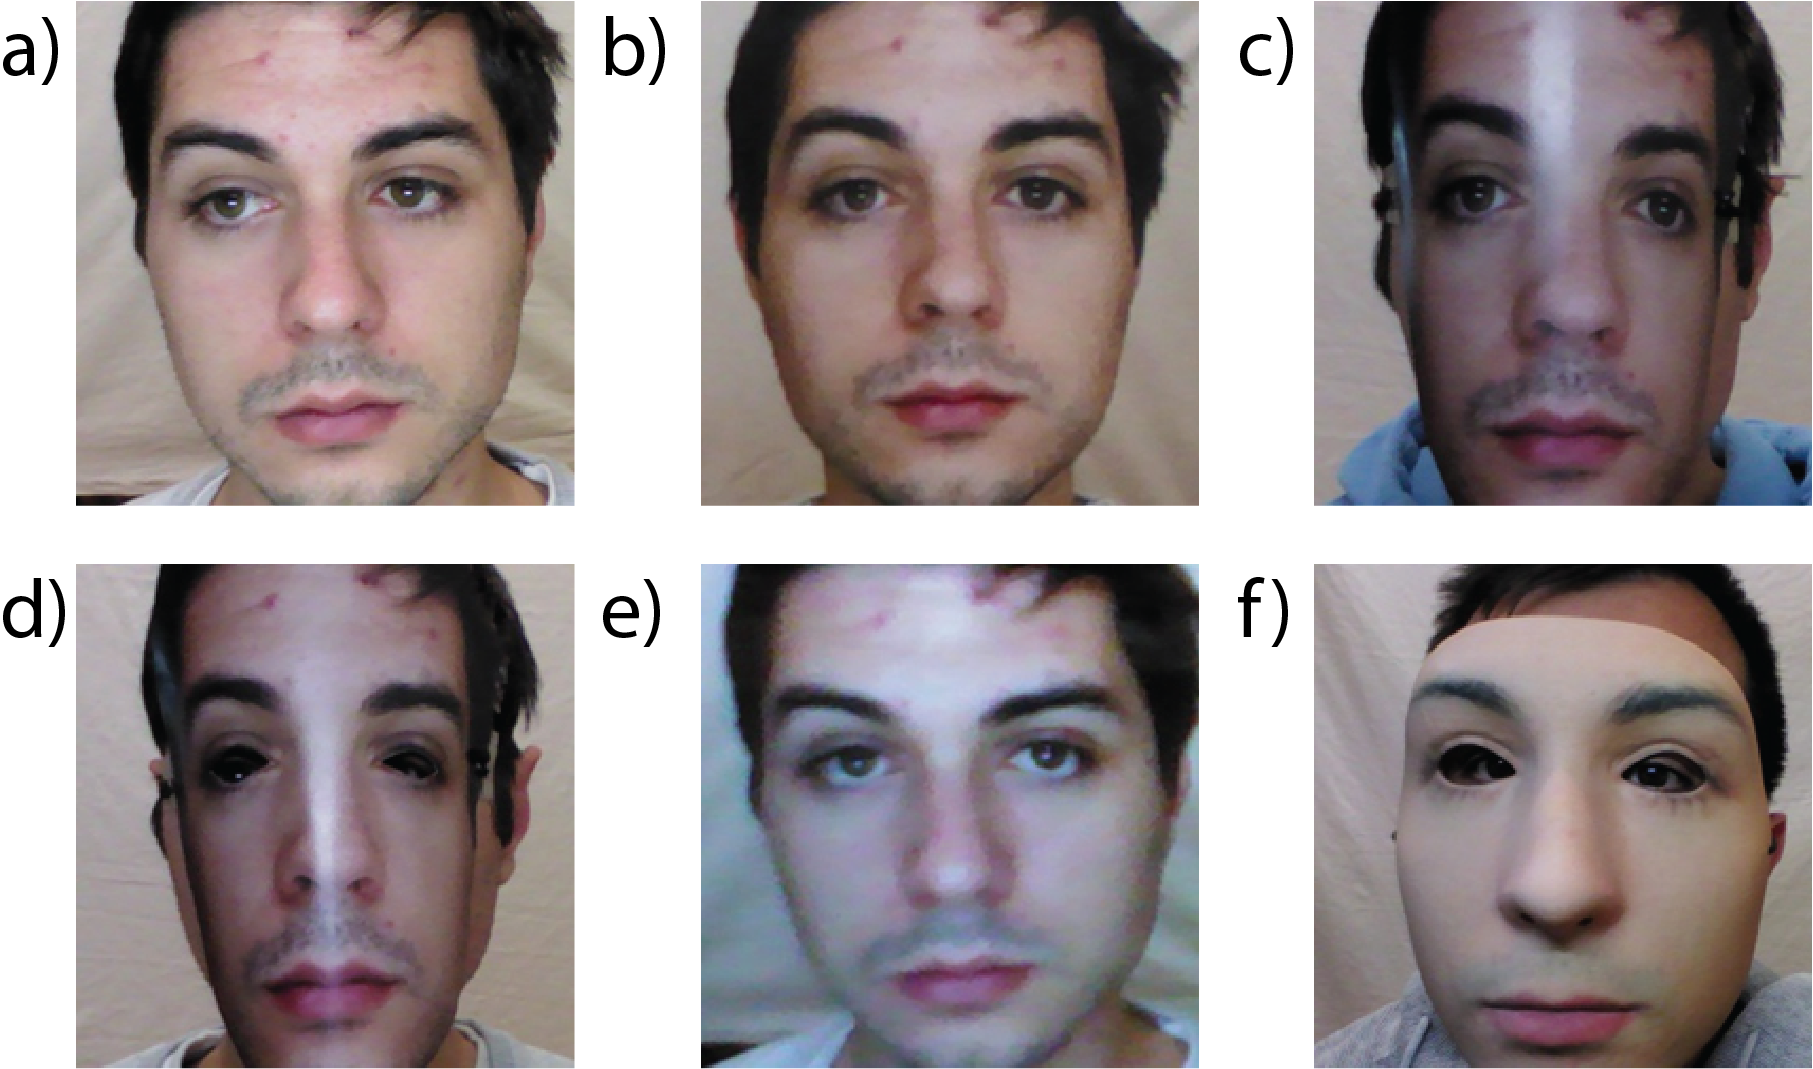
\includegraphics[width=1\textwidth]{ch-sistemasABC/images/ch-BBDDs/ATAQUES.png}
    \caption{Capturas \gls{bona-fide} y distintos ataques con la identidad de un mismo sujeto en \Gls{FRAV-Attack}. (a) \gls{bona-fide}, (b) \GLS{PAI} fotografía, (c) \GLS{PAI} máscara de cartón, (d) \GLS{PAI} máscara de cartón  sin ojos, (e)  \GLS{PAI} video y (f) \GLS{PAI} máscara $3$D.}
    \label{fig:DISTINTOS_ATAQUES_EN_FRAV_ATTACK}
\end{figure}

Aunque existe un gran número de publicaciones sobre detección de ataques de presentación, habitualmente tienen en cuenta pocos tipos de ataques diferentes y utilizan un único tipo de sensor para realizar las captura. \Gls{FRAV-Attack} se construyo con el objetivo de implementar y evaluar un método \GLS{PAD} multi-ataque y multi-sensor como el que se presenta en el Capitulo \ref{ch:PAD_MULTIATAQUE}. La base de datos incluye diferentes tipos de ataque y capturas realizadas con distintos tipos de sensores.

\begin{figure}[ht]
     \centering
     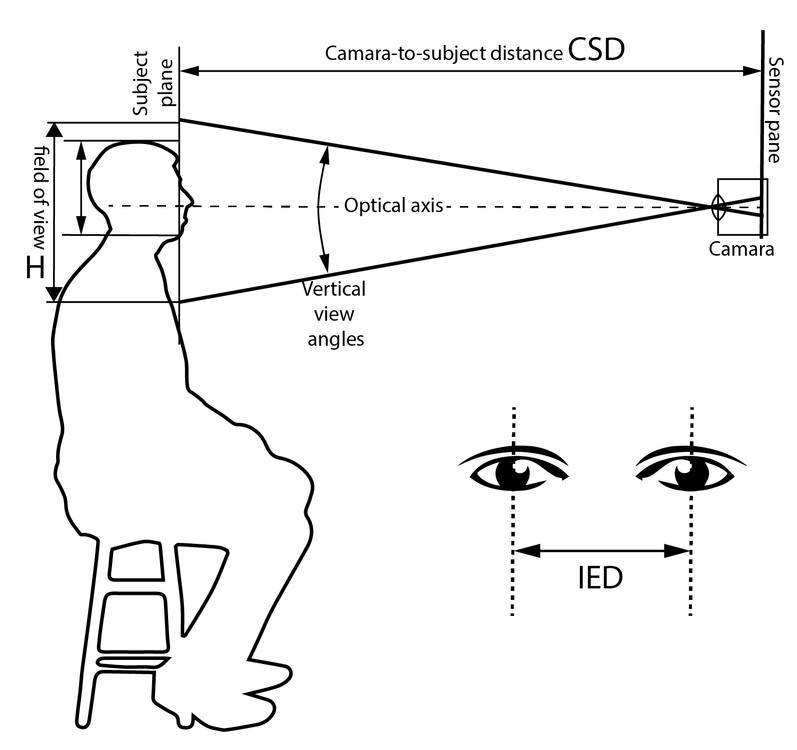
\includegraphics[width=0.6\textwidth]{ch-sistemasABC/images/ch-BBDDs/CAPTURA_ESTATICA.png}
     \caption{Esquema del proceso de captura de \Gls{FRAV-Attack}.}
     \label{fig:EsquemaCapturaFRAVAttack}
\end{figure}

La base de datos fue capturada por el grupo de investigación \GLS{FRAV} en un laboratorio de la universidad \GLS{URJC} bajo condiciones controlados de iluminación, de fondo y de pose. Para la iluminación se usaron dos tipos de iluminación en cada captura: luz halógena y luz infrarroja \GLS{IR}. Y de cada sujeto se capturaron tres poses: frontal, lateral derecha y lateral izquierda. La pose frontal cumple las normas fijadas en el estándar de \GLS{ICAO} Doc $9303$ \cite{doc20069303}) para documentos de viaje (ver Fig.\ref{fig:EsquemaCapturaFRAVAttack}), que recomienda una distancia al sensor \GLS{CSD} y una distancia intraocular \GLS{IED} (ver Tabla \ref{tab:distanciasICAO}).   

Entre los sujetos de la base de datos se incluyeron, tanto estudiantes como personal docente y de servicios de la propia universidad buscando una muestra lo más heterogénea posible. Finalmente la base de datos contiene 185 sujetos, 88 mujeres y 97 hombres, de edades comprendidas entre los 18 y los 53 años. Las capturas de un mismo sujeto se realizaron en una única sesión.

\begin{table}[t!]
    \centering
    \begin{tabular}{|l|c|c|} \hline
    \multicolumn{1}{|p{2cm}|}{} & \multicolumn{1}{|p{4cm}|}{\centering\textbf{IEC}} & \multicolumn{1}{|p{5cm}|}{\centering\textbf{CSD}} \\ \hline 
    \small{\textbf{Requerido}} & \textbf{IEC} $\geq 90$ mm  & $0.7 m\leq $ \textbf{CSD} $\leq 4$ m\\ \hline  \small{\textbf{Recomendado}} & \textbf{IEC} $\geq 120$ mm. & $1 m\leq $ \textbf{CSD} $\leq 2.5$ m\\ \hline 
    \end{tabular}
    \caption{\GLS{CSD} Distancia entre la persona y el sensor de captura y \GLS{IED} distancia intraocular,  requeridas y recomendadas por el estándar \GLS{ICAO} Doc $9303$ \cite{doc20069303}.}
    \label{tab:distanciasICAO}
\end{table}

%%%% ATAQUES CONTEMPLADOS  %%%%%%
\subsection{Ataques}\label{subsec:PAI-FRAV-Attack}


\begin{figure}[t]
    \centering
    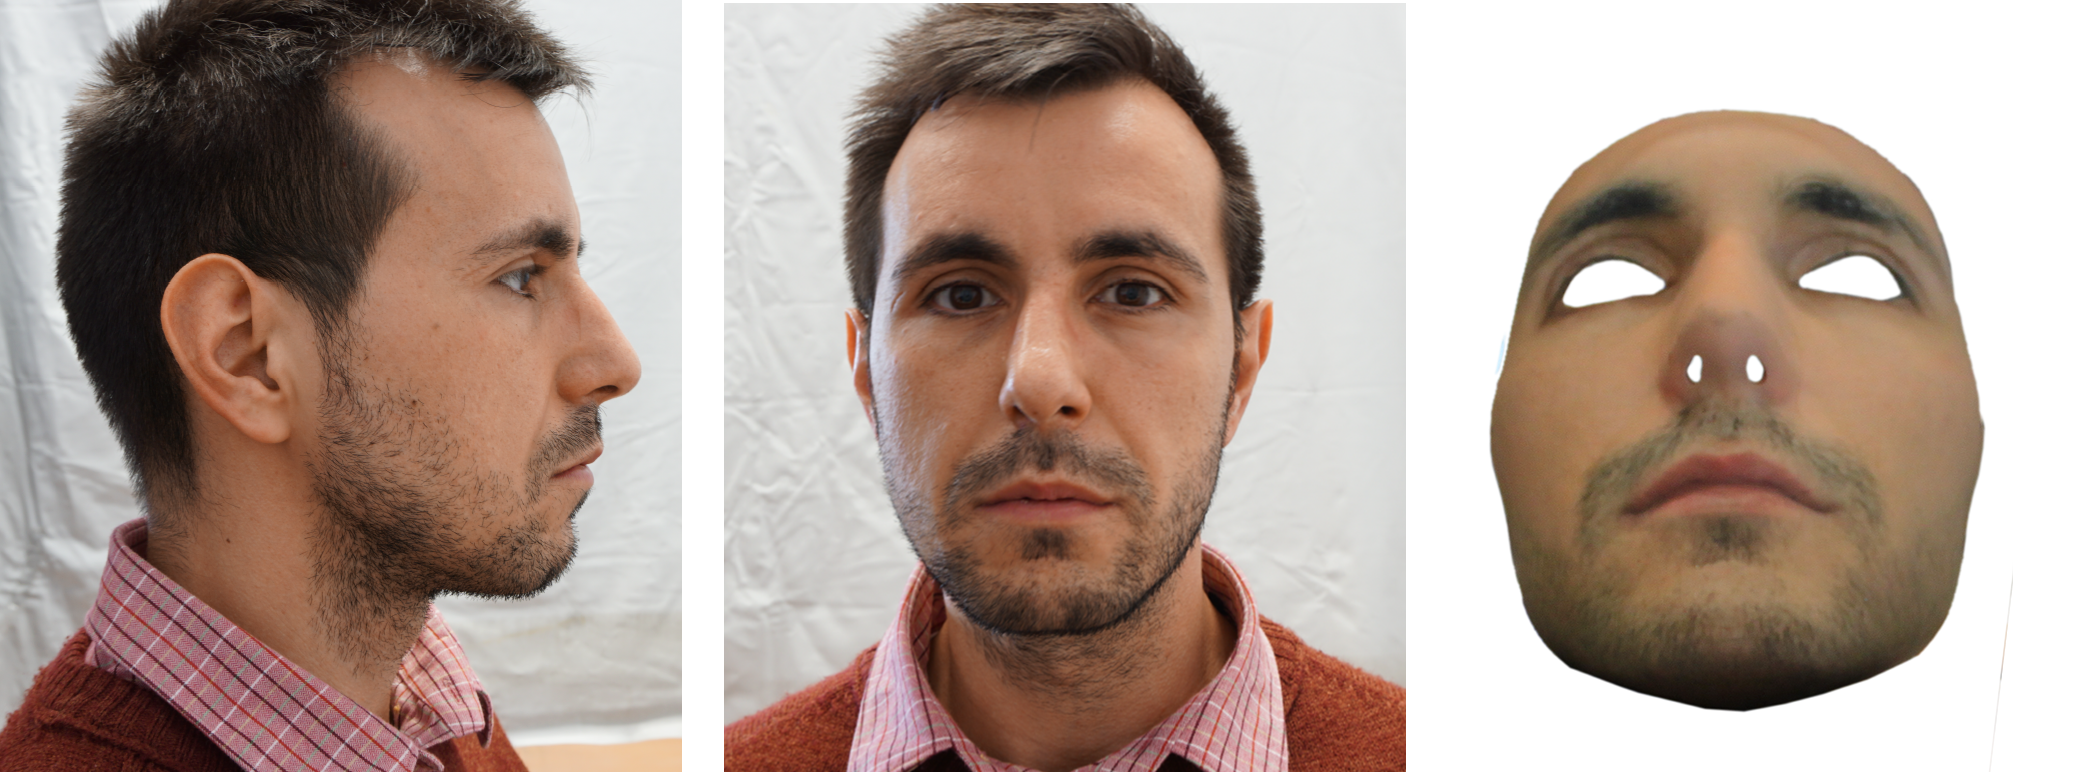
\includegraphics[width=1\linewidth]{ch-sistemasABC/images/ch-BBDDs/CONSTRUCCION_MASCARAS_3D.png}
    \caption{Máscara $3$D impresa a partir de un modelo creado por fotometría.}
    \label{fig:ConstrucionMascara3D}
\end{figure}

Además de capturas \gls{bona-fide}, se simularon ataques de presentación con $5$ tipos de \GLS{PAI} con la identidad de cada sujeto: fotografía, mascara de cartón, mascara de cartón con ojos recortados o \textit{eyeless}, pantalla y máscara $3$D (ver Fig. \ref{fig:DISTINTOS_ATAQUES_EN_FRAV_ATTACK}). A continuación se explica en que consisten los ataques con cada uno de estos \GLS{PAI}:

\medskip
\textbf{PAI fotografía} 

Consiste en presentar al sensor una fotografía impresa con la imagen del sujeto a suplantar.Se trata de una ataque simple pero muy efectivo en sistemas que no cuentan con ningún tipo de \GLS{PAD}

\medskip
\textbf{PAI máscara cartón} 

Consiste colocarse una máscara de cartón que reproduce la cara del sujeto a suplantar. A diferencia del ataque con fotografía al generar un volumen alrededor de la cara, resulta un ataque menos detectable que una fotografía plana, para sistemas \GLS{PAD} basados en profundidad.
    
\medskip
\textbf{PAI máscara cartón \textit{eyeless}}

Consiste también en llevar una máscara de cartón con la cara del sujeto a suplantar, pero en este caso los ojos de la máscara se recortan para engañar a \gls{liveness detection} \GLS{PAD} basados en la de detección de parpadeo (ver apartado \ref{sec:TiposPAD}).

\medskip
\textbf{PAI vídeo}

Consiste presentar ante el sensor la pantalla de un dispositivo electrónico que reproduce un vídeo del sujeto a suplantar. Este tipo \GLS{PAI} es también capaz de engañar a métodos \gls{liveness detection} \GLS{PAD} (ver apartado \ref{sec:TiposPAD}).

\medskip
\textbf{PAI máscara 3D}

Consiste en colocarse una máscara rígida del sujeto a suplantar.Las máscaras empleadas en \textit{\Gls{FRAV-Attack}} fueron fabricadas por la empresa \textit{ThatsMyFaces} \cite{ThatsMyFaceOnline}, mediante la impresión $3$D de un modelo estimado por fotogrametría con las vistas frontal y lateral del sujeto (ver Fig. \ref{fig:ConstrucionMascara3D}). Si bien este tipo de máscaras resultan cada día más asequibles, en \Gls{FRAV-Attack} sólo se incluyeron ataques con $10$ máscaras de este tipo. debido al coste que supondría la impresión de mascaras para los $185$ sujetos. Este tipo de máscaras es uno de los más peligrosos  ya que consiguen engañar a sistemas automáticos muy sofisticados que usan cámaras de profundidad o escáneres $3$D \cite{erdogmus2014spoofing}, \cite{jia2019survey} \cite{li2016generalized}.
\medskip

%%%%%%%%% SENSORES  %%%%%%%%%%%%
\subsection{Dispositivos de captura}\label{subsec:Dispositivos-FRAV-Attack}

\begin{figure}[t!]
\centering
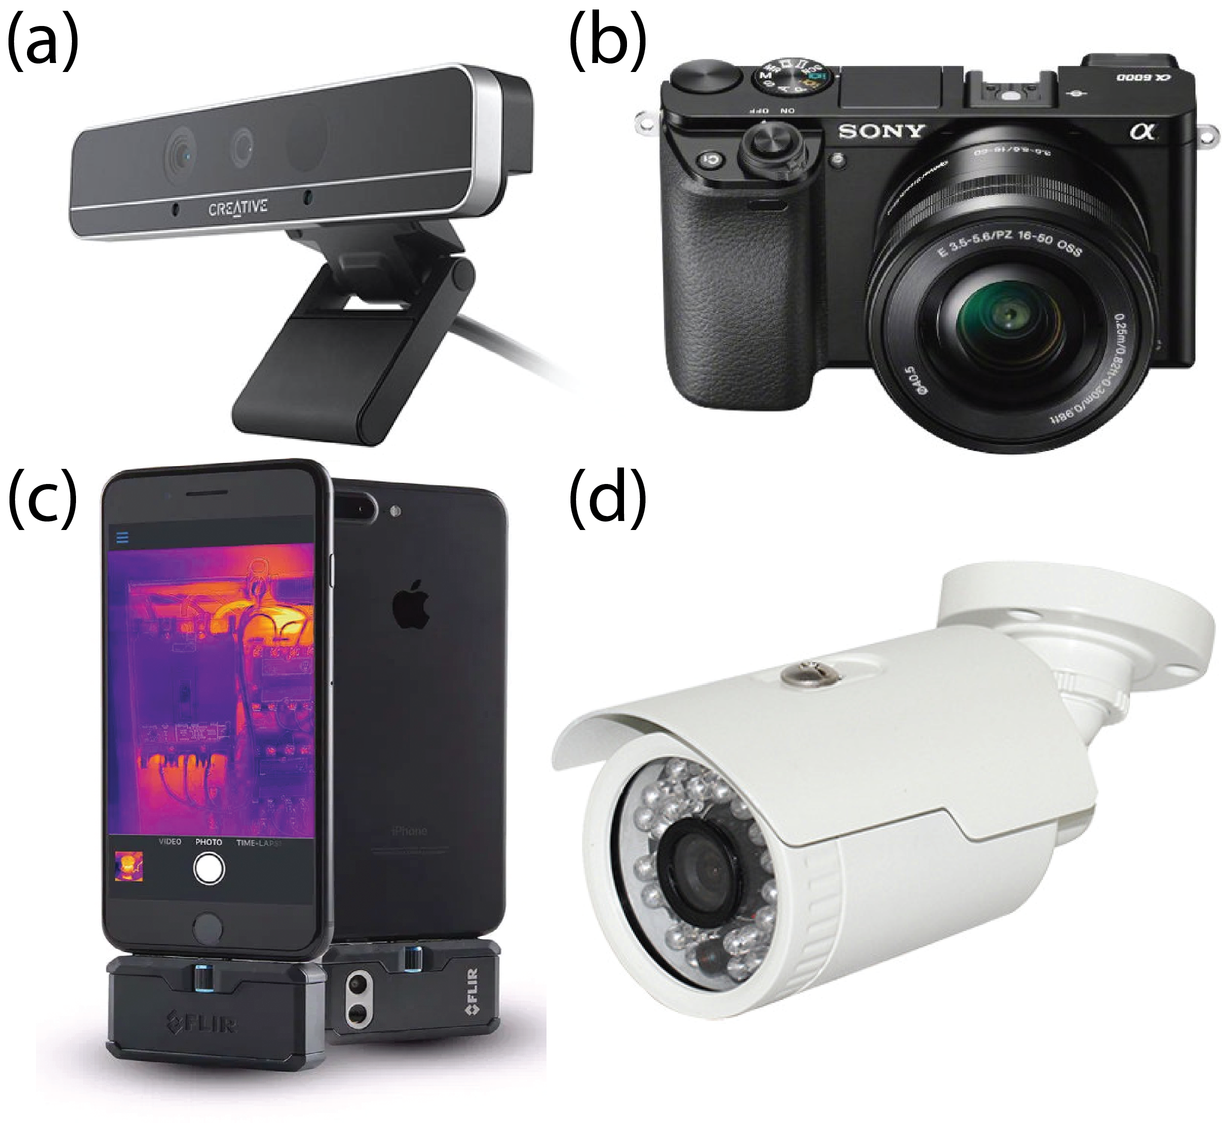
\includegraphics[width=0.6\textwidth]{ch-sistemasABC/images/ch-BBDDs/SENSORES.png}
    \caption{Dispositivos de captura de la base de datos \textit{\Gls{FRAV-Attack}}: (a) \textit{Intel\textsuperscript{\textregistered}RealSense\textsuperscript{\texttrademark}}. (b) \textit{Sony\textsuperscript{\textregistered}$\alpha6000$}. (c) \textit{\GLS{FLIR}-One} y (d) \textit{SurveillanceCam}}
    \label{fig:SENSORES}
\end{figure}

Para las capturas tanto de los \gls{bona-fide} como de los ataques de \Gls{FRAV-Attack}, se emplearon cuatro dispositivos, algunos de ellos con varios sensores que permiten capturas en rangos del espectro, diferentes al visible: \textit{Intel\textsuperscript{\textregistered}RealSense\textsuperscript{\texttrademark}}, \textit{Sony\textsuperscript{\textregistered}$\alpha6000$}, \textit{SurveillanceCam} y \textit{\GLS{FLIR}-One} (ver Fig.\ref{fig:SENSORES}). A continuación se especifican las características de cada uno de los sensores y de las capturas realizadas con ellos. 

%REALSENSE
\medskip
\textbf{Intel\textsuperscript{\textregistered}RealSense\textsuperscript{\texttrademark}}:

La cámara RealSense F$200$ \cite{RealSenseOnline} dispone de sensor \GLS{RGB} y también de un sensor \GLS{IR} que permite obtener información de profundidad ($2.5$D) mediante la lectura un un patrón de luz estructurada emitida por un proyector infrarrojo.

En \\Gls{FRAV-Attack}, con esta cámara, se grabaron vídeos de 400 fotogramas, uno con el \gls{bona-fide} y $5$ con los \GLS{PAI} correspondientes de cada sujeto. De cada fotograma se extrajeron: la imagen \GLS{RGB} con una resolución de $1920\times1080$, la imagen \GLS{IR} con una resolución de $640\times480$ y la matriz de profundidades, también con $640\times480$ de resolución. (aproximadamente $1$ millón imágenes en total). En Fig. \Ref{fig:USUARIOS_RELASENSE} se pueden ver las segmentación facial de tres sujetos de \Gls{FRAV-Attack}, en cada una de estas imágenes.

%SONY
\medskip
\textbf{Sony\textsuperscript{\textregistered}$\mathbf{\alpha6000}$}

Cámara fotográfica con un sensor \GLS{RGB} de alta resolución capaz de capturar imágenes de $24.3$ MP y vídeos ($4$HD) a $1080$. 

Para \Gls{FRAV-Attack} con este dispositivo se capturaron, de cada sujeto, tres imágenes \gls{bona-fide} de $6000\times4000$ píxeles con pose frontal, perfil derecho y perfil izquierdo. Y una imagen también de $6000\times4000$ píxeles de cada uno de los \GLS{PAI} (aproximadamente $1500$ imágenes). 

Gracias a la calidad de las imágenes obtenidas con este sensor se han utilizado para la construcción de los diferentes \GLS{PAI} (ver Fig. \ref{fig:ConstrucionMascara3D}). 

%FLIR TERMICO
\medskip
\textbf{\gls{FLIR}-One} 

La cámara \gls{FLIR}-One \cite{FLIROnline} tiene de un sensor \GLS{RGB} y otro térmico capaz de capturar la temperatura emitida por los objetos en el de infrarrojo medio con un rango de temperaturas entre -$4^{\circ}$F to $248^{\circ}$F (-$20^{\circ}$C to $120^{\circ}$ C). 

En \Gls{FRAV-Attack} se tomaron tres capturas con el \gls{bona-fide} de cada sujeto en pose frontal, perfil derecho y perfil izquierdo, y una captura de los \GLS{PAI} correspondientes. Cada captura de este dispositivo genera dos matrices de $160\times120$ con la información térmica: \textit{ThermalLinearFlux} y \textit{ThermalRadiometricKelvin}, y dos imágenes \GLS{RGB} de $640\times480$ píxeles: \textit{VisualJPEGImage}, en formato \GLS{JPEG} y \textit{VisualYCbCr888Image}, en formato \Gls{YCbCr} (aproximadamente $6000$ imágenes).  

A las imágenes generadas se les puede aplicar paletas de color atendiendo a las matrices de temperatura para analizar determinadas propiedades térmicas: \textit{Arctic}, \textit{Coldest}, \textit{Hottest}, \textit{Contrast}, \textit{Gray}, \textit{Iron}, \textit{Lava}, \textit{Rainbow}, \textit{Whell} (ver Fig.\ref{fig:DISTINTAS_PALETAS_TERMICAS} y Fig. \ref{fig:DISTINTOS_ATAQUES_DISTINTAS_PALETAS}).

%INFRARROJO
\medskip
\textbf{Surveillance-Cam}

% \begin{figure}[t!]
% \centering
% 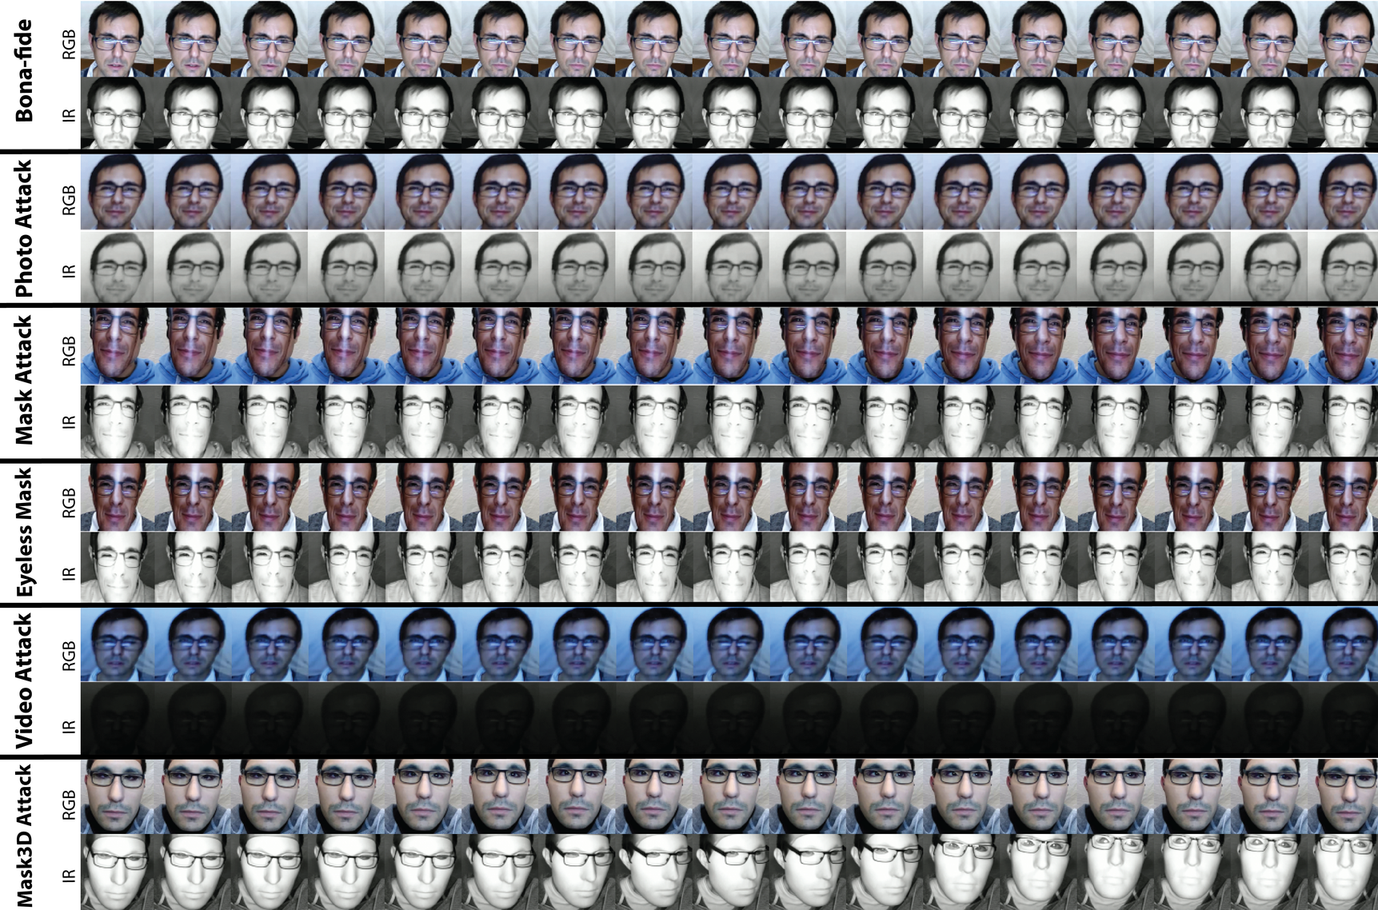
\includegraphics[width=1\textwidth]{ch-sistemasABC/images/ch-BBDDs/MUESTRAS_IR.png}
%     \caption{Fotogramas de los vídeos de \textit{\Gls{FRAV-Attack}} con el cámara \textit{SurveillanceCam}.}
%     \label{fig:MUESTRAS_IR}
% \end{figure}

El dispositivo \textit{Surveillance-Cam} es una cámara de alta resolución, empleada en labores de vídeo-vigilancia, capaz de capturar imágenes y vídeos, en\GLS{RGB} y en \GLS{IR}. Además dispone de un sistema integrado de iluminación infrarroja.

En \Gls{FRAV-Attack} de cada sujeto se grabaron vídeos de $400$ fotogramas, uno con el \gls{bona-fide} y 5 con los \GLS{PAI} correspondientes. De cada fotograma se extrajeron: la imagen \GLS{RGB} y la \GLS{IR}, ambas con una resolución $1920\times1080$ píxeles. (casi un 1 millón imágenes en total). En Fig. \Ref{fig:MUESTRAS_IR} se pueden ver imágenes extraídas de los vídeos de un sujeto de \Gls{FRAV-Attack}.


\begin{landscape}
\begin{figure}[t!]
\centering
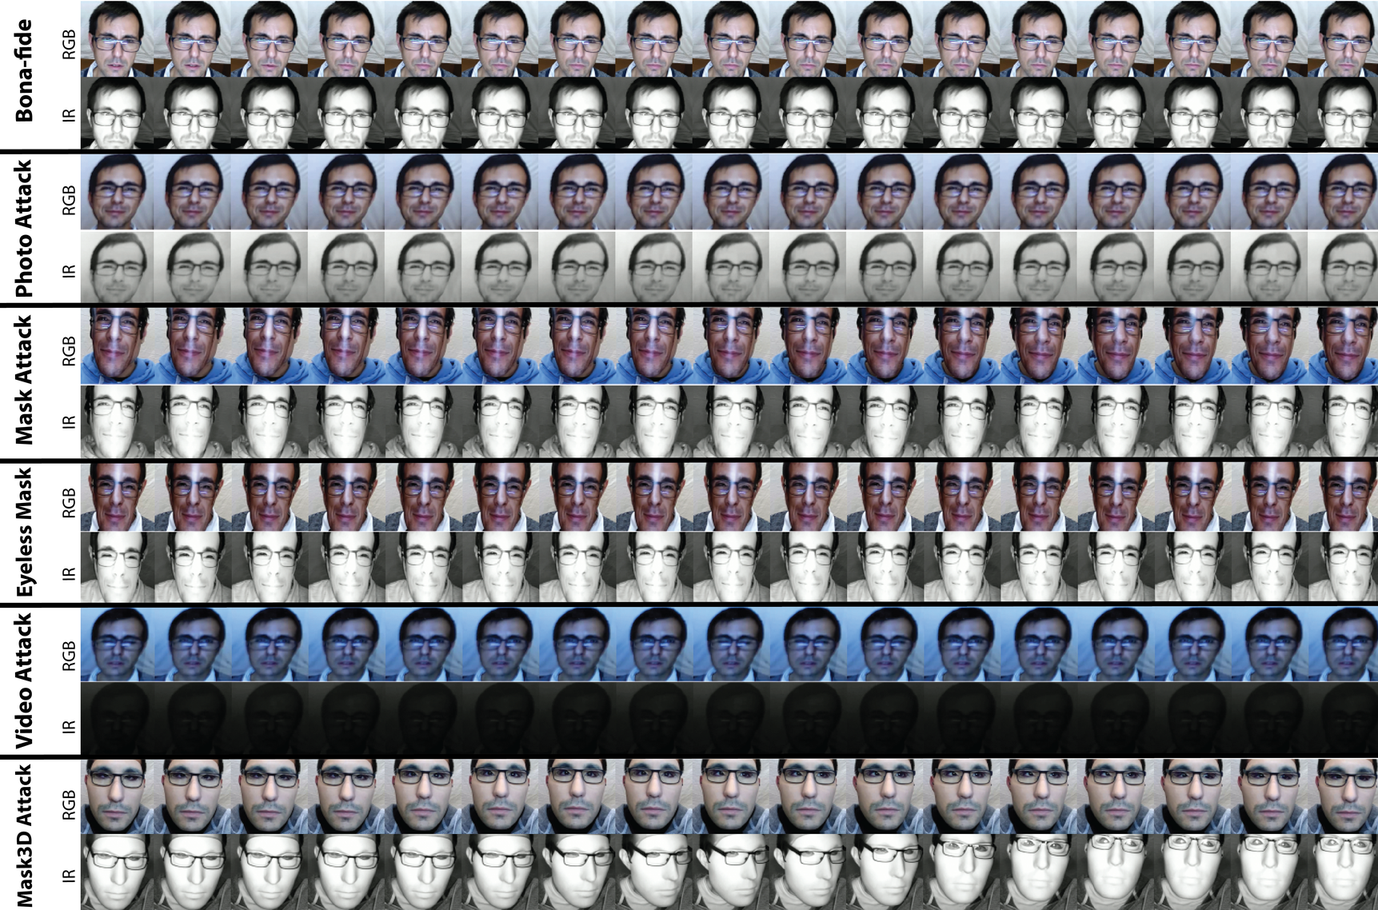
\includegraphics[width=1.4\textwidth]{ch-sistemasABC/images/ch-BBDDs/MUESTRAS_IR.png}
    \caption{Fotogramas de los vídeos de \Gls{FRAV-Attack} con el cámara \textit{SurveillanceCam}.}
    \label{fig:MUESTRAS_IR}
\end{figure}
\end{landscape}

\begin{landscape}
\begin{figure}
    \centering
    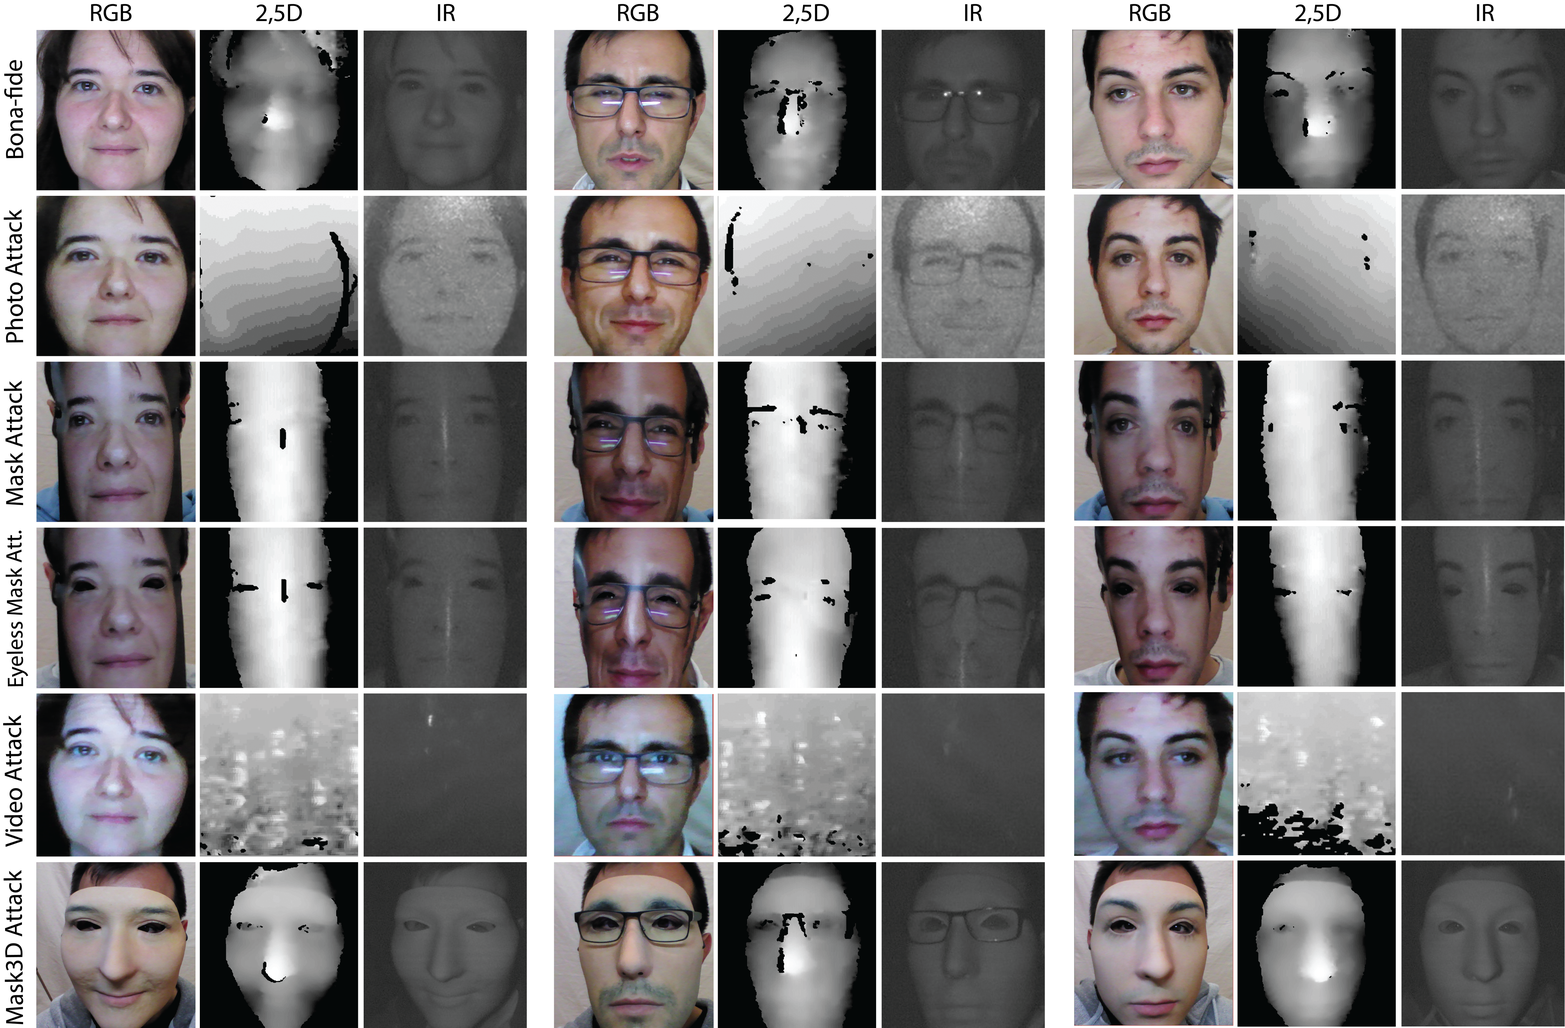
\includegraphics[width=1.4\textwidth]{ch-sistemasABC/images/ch-BBDDs/USUARIOS_REAL_SENSE.png}
    \caption{Capturas de \Gls{FRAV-Attack} con el cámara \textit{Intel-RealSemse}.}
    \label{fig:USUARIOS_RELASENSE}
\end{figure}
\end{landscape}

\begin{landscape}
 \begin{figure}
  \centering
  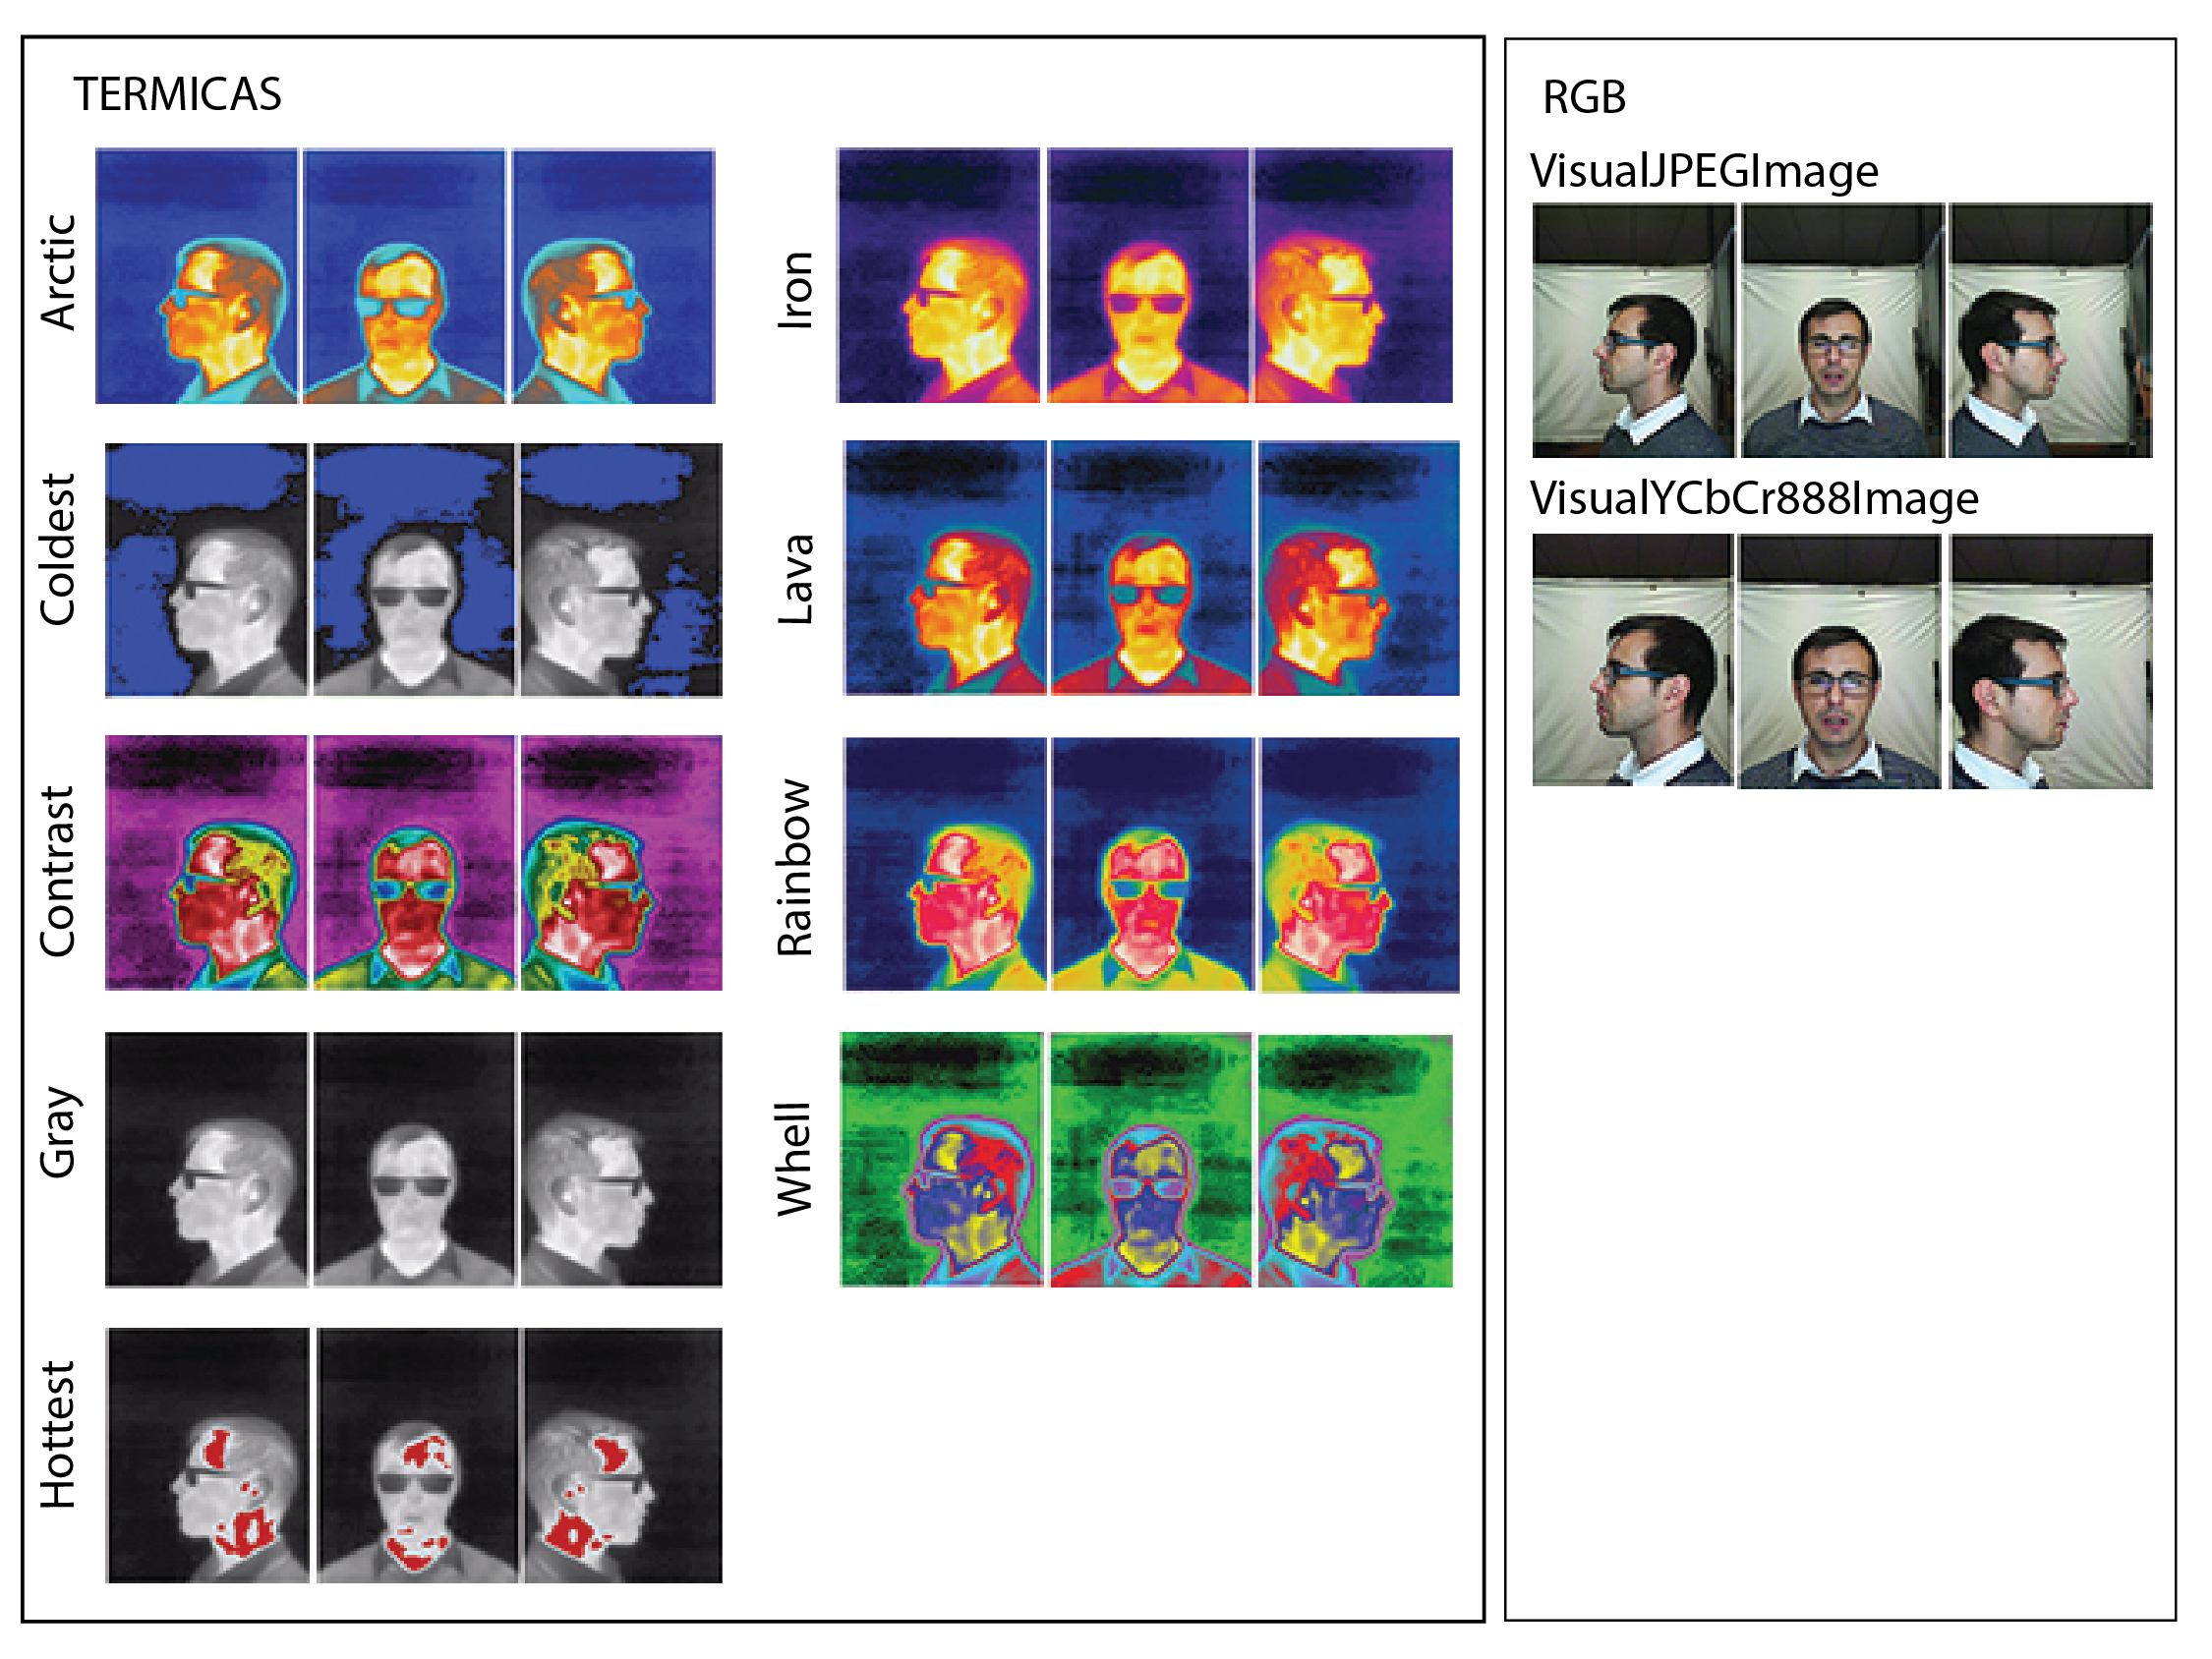
\includegraphics{ch-sistemasABC/images/ch-BBDDs/DISTINTAS_PALETAS_TERMICAS.png}
        \caption{Capturas de \Gls{FRAV-Attack} con el sensor térmico \GLS{FLIR}}
        \label{fig:DISTINTAS_PALETAS_TERMICAS}
 \end{figure}
\end{landscape}

\begin{landscape}
 \begin{figure}
  \centering
  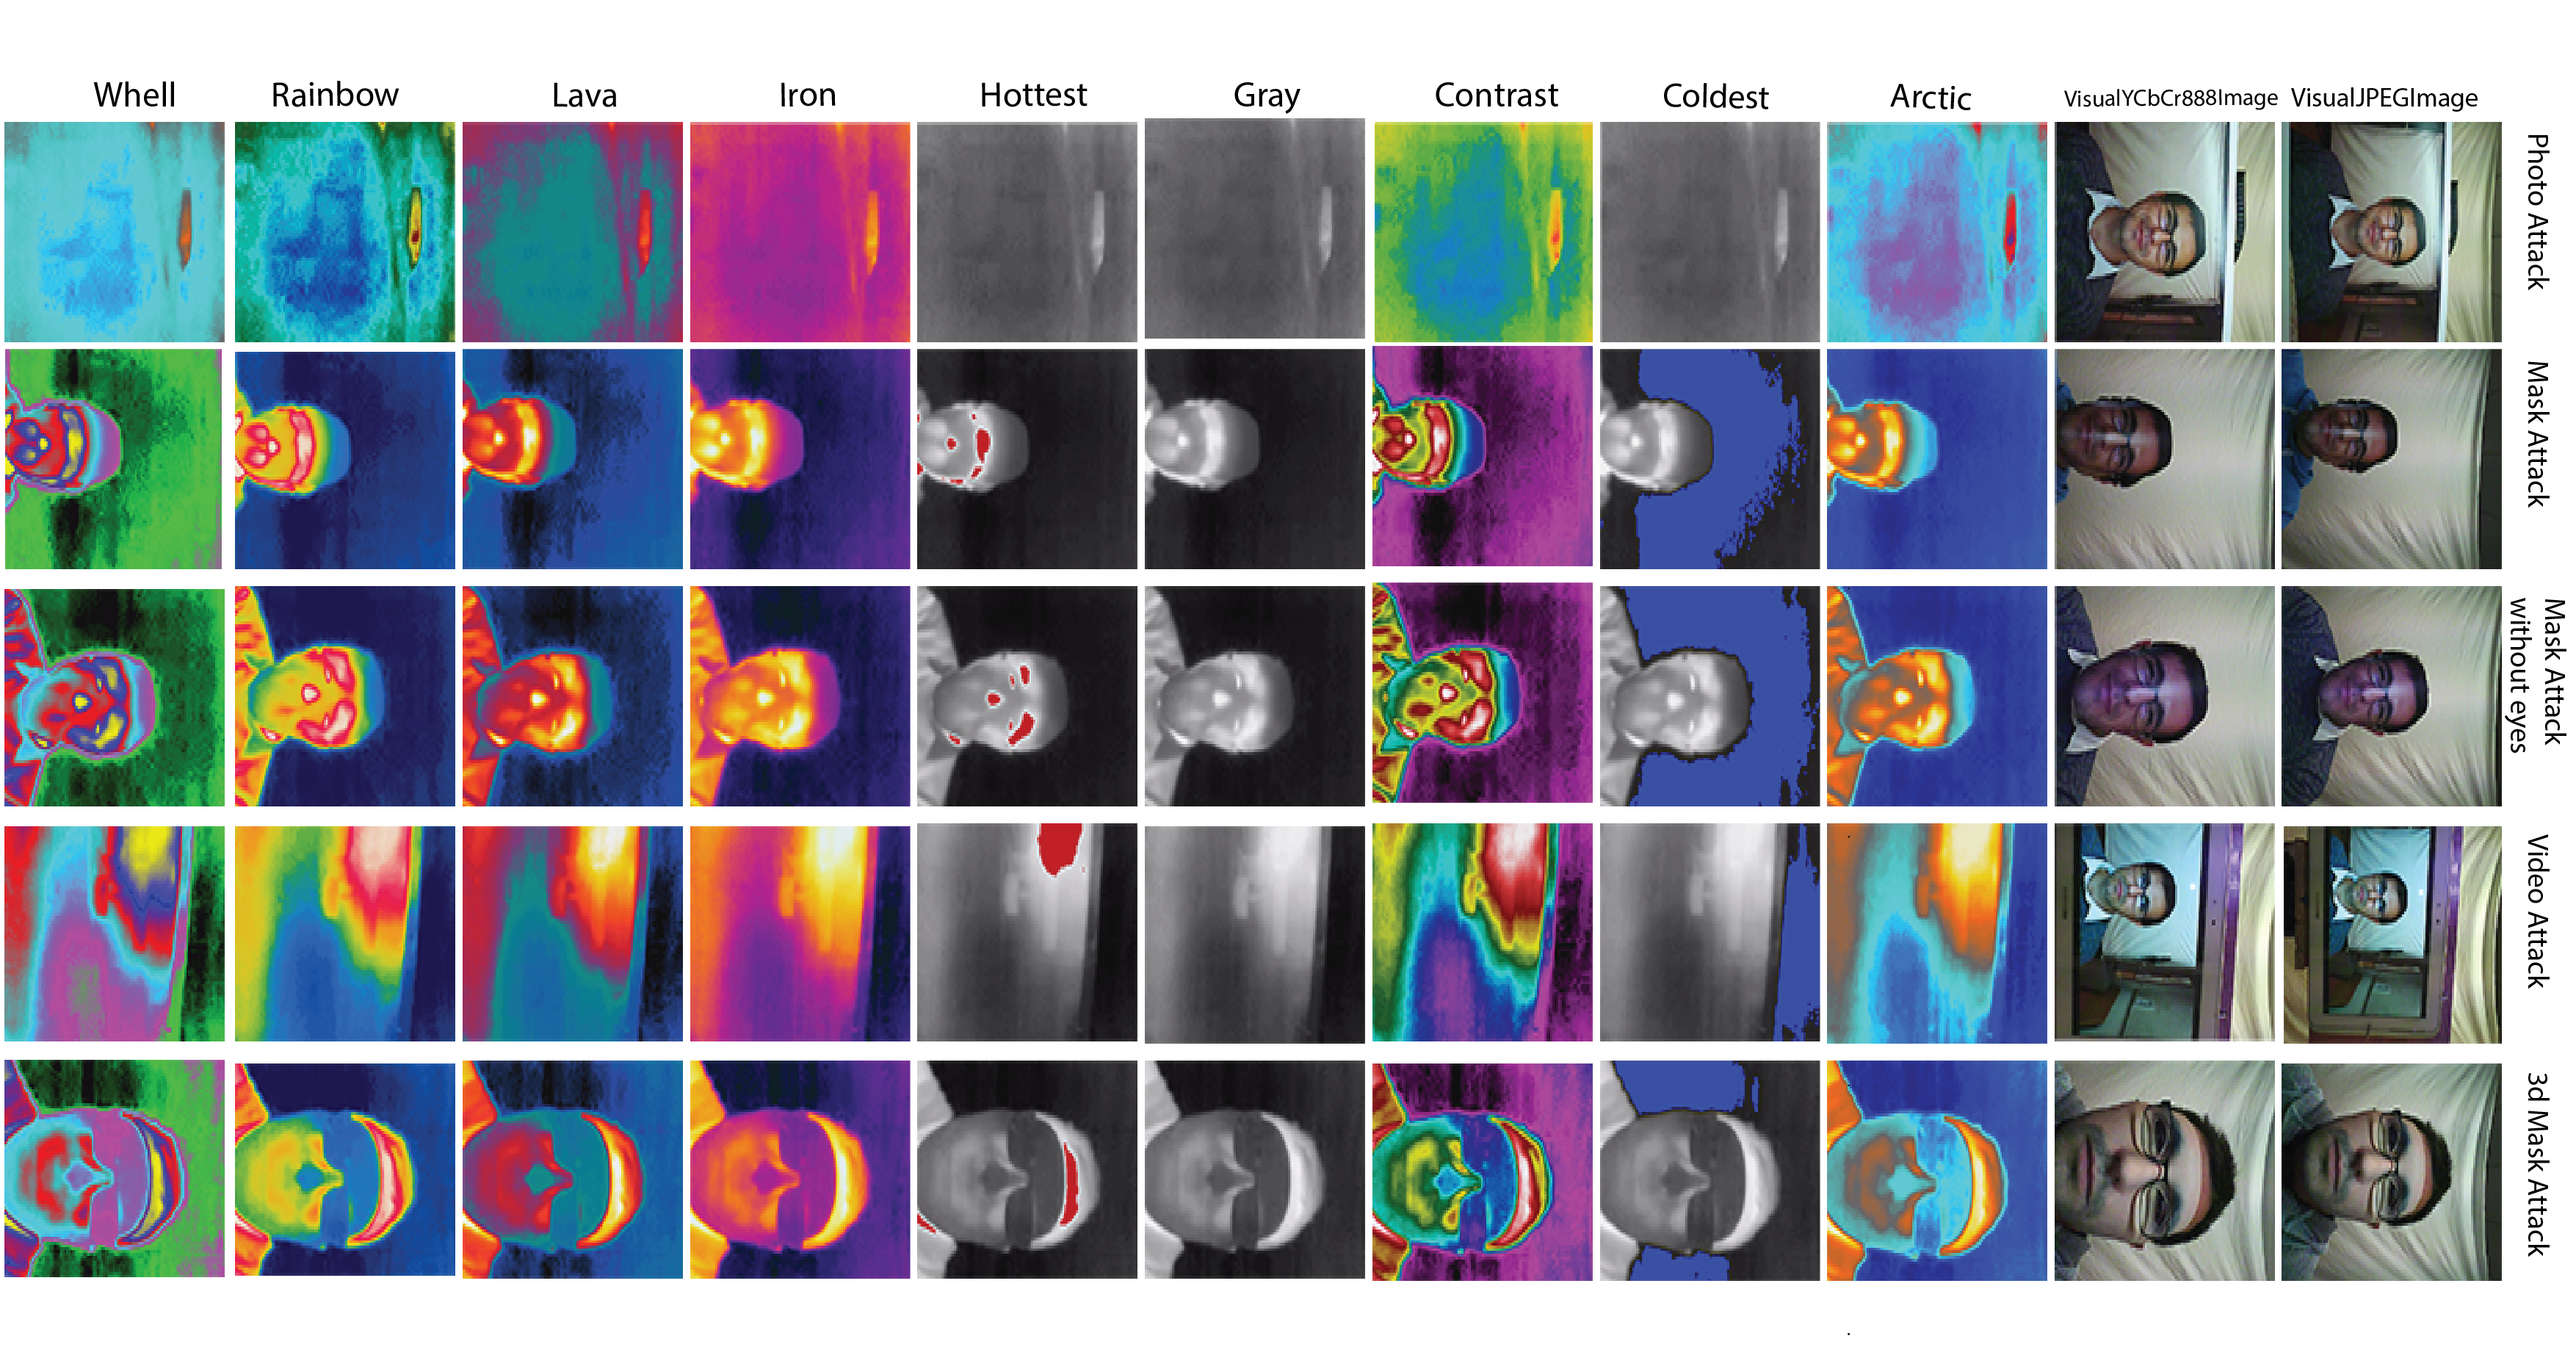
\includegraphics[width=1.5\textwidth]{ch-sistemasABC/images/ch-BBDDs/DISTINTOS_ATAQUES_DISTINTAS_PALETAS.png}
        \caption{Capturas de \Gls{FRAV-Attack} con el sensor térmico \GLS{FLIR}. Con cada uno de los ataques contemplados.}
        \label{fig:DISTINTOS_ATAQUES_DISTINTAS_PALETAS}
 \end{figure}
\end{landscape}


%%%%%%%%%%%%%%%%%%%%% BASES DE DATOS PARA SISTEMAS ABC  %%%%%%%%%%%%%%%%%%%%%%% 
\section{Bases de datos para sistemas ABC}\label{sec:BBDD-ABC}

En esta sección se presentan dos bases de datos capturadas por dispositivos \GLS{ABC} en cruces de fronteras reales. \Gls{FRAV-ABC} que incluye únicamente las imágenes que forman parte de un cruce \gls{bona-fide}: imágenes \gls{chip} e imágenes \gls{vivo bona-fide}. Sin embargo en \Gls{FRAV-ABC-Attack} considera además ataques de presentación en las imágenes \gls{vivo}. También en \Gls{FRAV-ABC-Attack} un subconjunto de los datos se capturó en un sistemas \GLS{ABC} \textit{<<Segregated Two Step>>}, lo que implica dos procesos de verificación biométrica. es decir dos capturas \gls{vivo}. En el apartado \ref{subsec:FRAV-ABC-ATTACK-DOS_PASOS} se explica el formato y las características de este subconjunto de datos.

El acceso a cruces de fronteras reales está muy controlado y limitado por razones de seguridad. La posibilidad de capturar los datos descritos en esta sección fue gracias la participación del grupo de investigación \GLS{FRAV} de la universidad \GLS{URJC} en el proyecto europeo FP$7$ \GLS{ABC4EU}, donde colaboró en la implantación de prototipos de sistemas \GLS{ABC} en fronteras aeroportuarias, fronteras terrestres y fronteras marítimas.

Se realizó una experiencia piloto en el Adolfo Aeropuerto Suárez Madrid-Barajas T$4$-S internacional terminal de llegadas en diciembre de $2016$. Este aeropuerto, que sirve a la capital de España y al centro de la Península Ibérica, es el aeropuerto más concurrido de España, y el quinto en Europa y el $24$º en el mundo en cuanto al tráfico de viajeros. En $2015$ alcanzó un de casi $47$ millones de viajeros \cite{ACI2016}.

%%%%%%%%%%%%%%%%%%%%% FRAV ABC  %%%%%%%%%%%%%%%%%%%%%%% 
\subsection{FRAV-ABC}\label{subsec:FRAV-ABC}

% \Figure[ht]()[width=.9\linewidth]{images/FRAV-ABC-Images.png}
%  {Examples of \textit{FRAV-ABC} data set images. Passport \textit{chip} images (top) and snap-shot images taken in the border scenario (bottom).\label{fig:SAMPLES-FRAV-ABC1}}

\begin{figure}[ht]
     \centering
     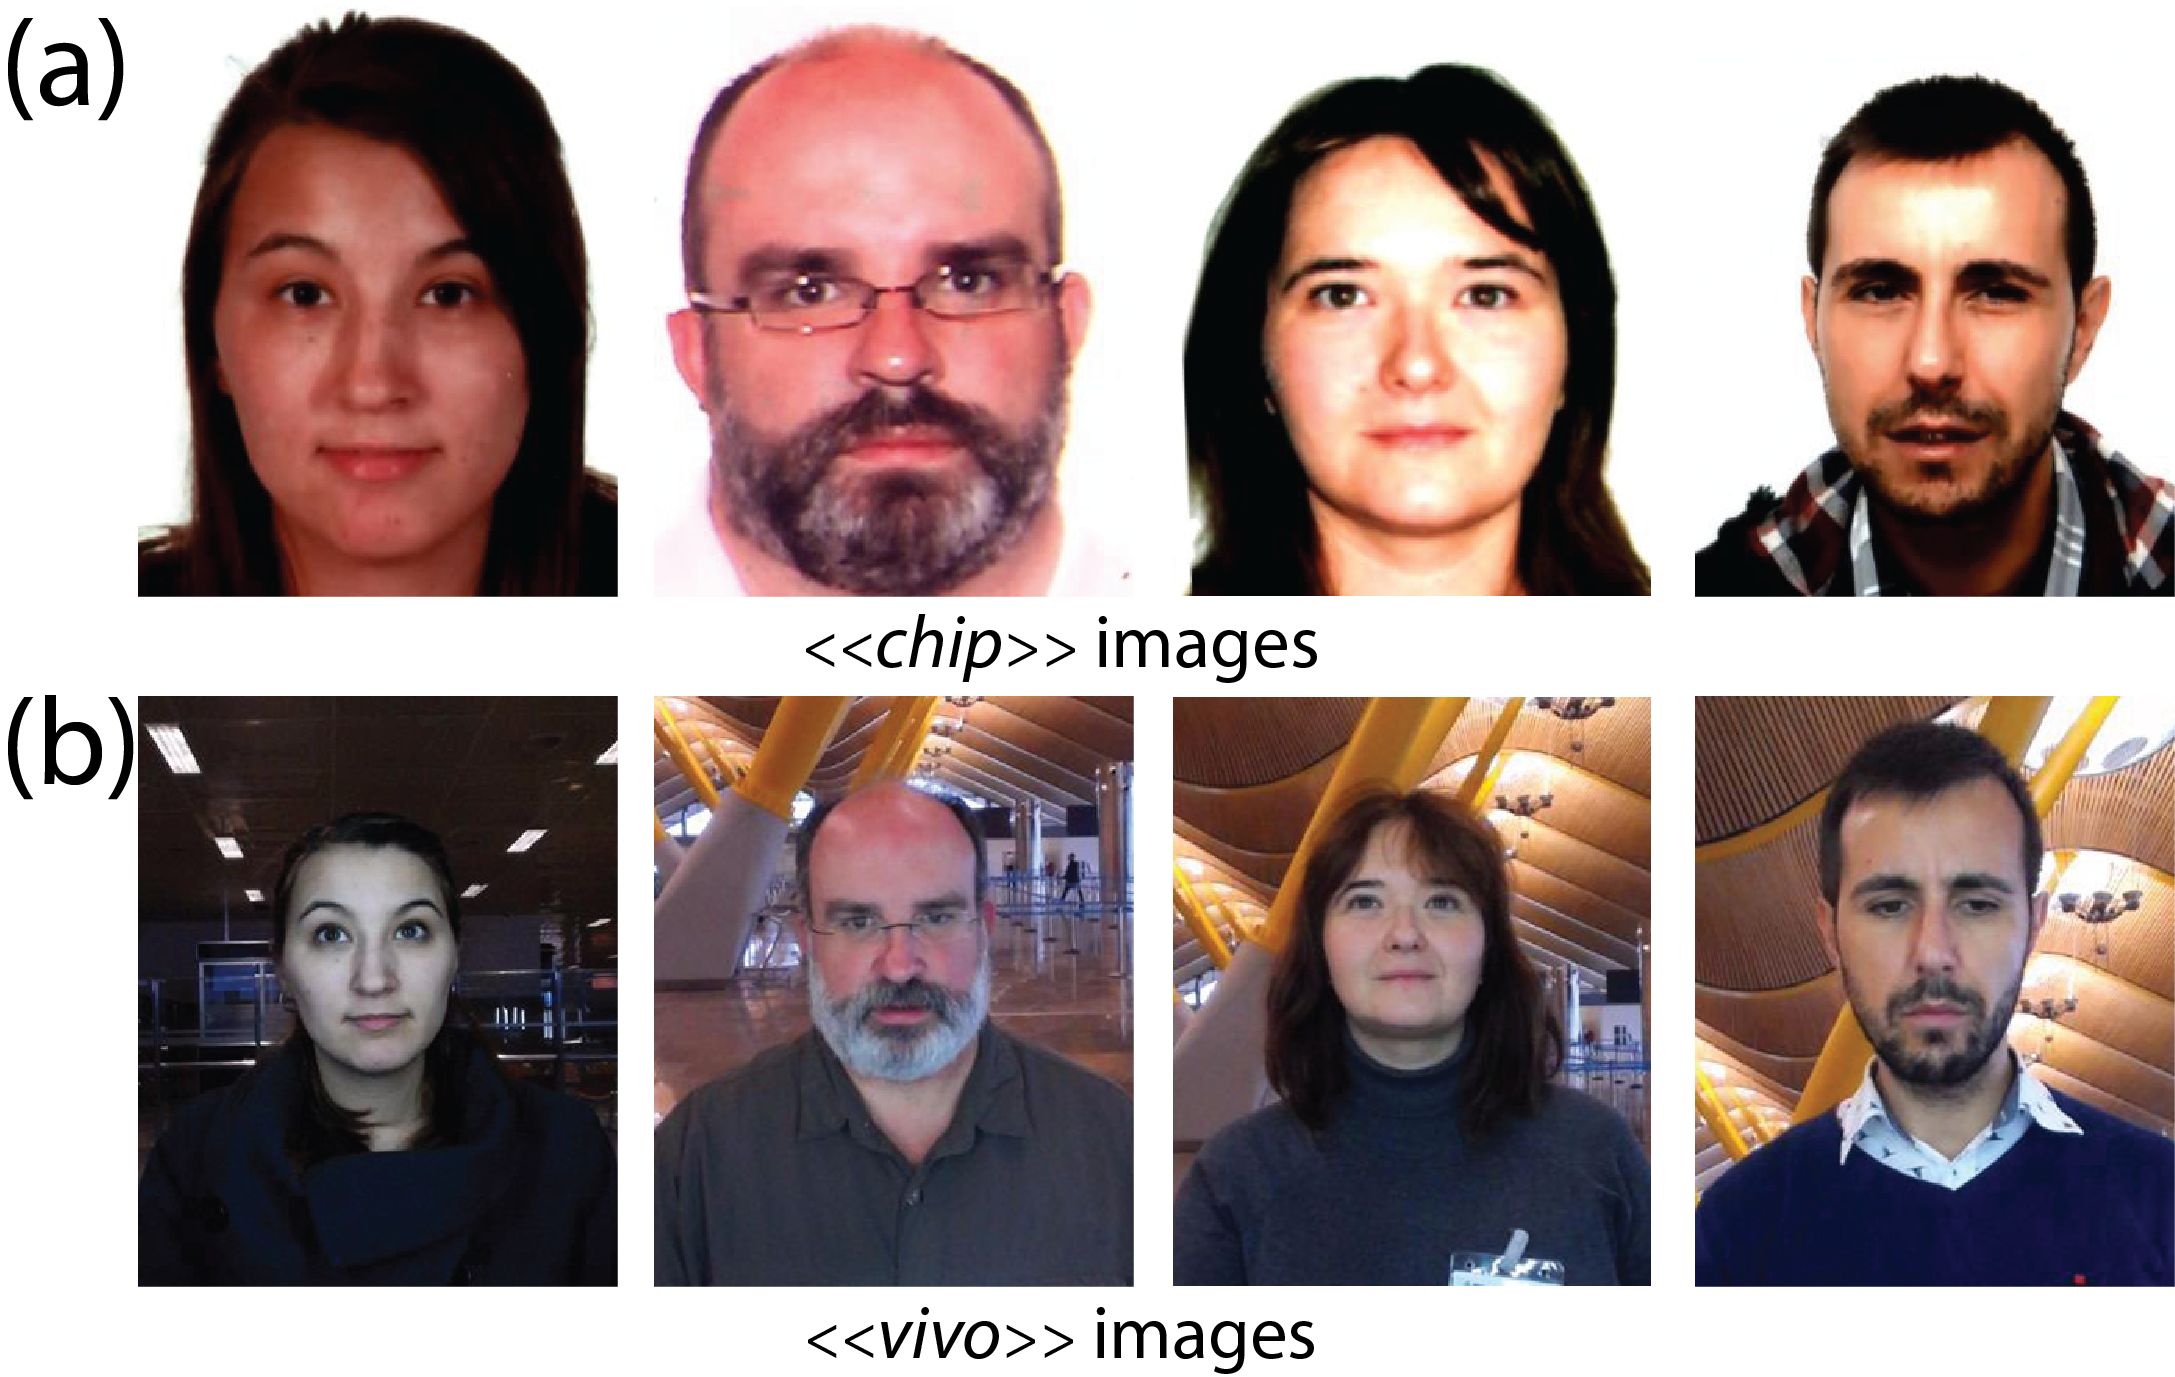
\includegraphics[width=0.8\textwidth]{ch-sistemasABC/images/ch-BBDDs/CHIP_VIVO_IMAGENES.png}
     \caption{Imágenes de sujetos de la base de datos \textit{\Gls{FRAV-ABC}}. (a) Imágenes del \gls{chip} del \gls{e-passport} y (b) Imágenes \gls{vivo} adquiridas por un sistema \GLS{ABC} en un cruce de fronteras real.}
     \label{fig:SAMPLES-FRAV-ABC1}
\end{figure}

En este apartado se describe la base de datos \Gls{FRAV-ABC}\footnote{La base de datos \Gls{FRAV-ABC} fue diseñada y recopilada por el grupo de investigación \GLS{FRAV} de la \GLS{URJC}\cite{urjcOnline} gracias a la colaboración de este grupo en el proyecto \GLS{ABC4EU}\cite{ABC4EUOnline} durante la implantación de sistemas \GLS{ABC} pilotos, en la terminal T$4$ en el Aeropuerto Alfonso Suarez Madrid-Barajas y en el puerto marítimo de Algeciras.}, compuesta por 1185 sujetos, 640 mujeres y 530 hombres, con un rango de edades entre 18 y 74 años. El $70$\% oscilaba entre $25$ y $50$ años de edad. De cada sujeto se dispone de dos imágenes: Una imagen con características similares a las almacenadas en los \gls{eMRTD} conocida como \gls{chip} y una imagen capturada en un dispositivo \GLS{ABC} en un cruce de fronteras real, conocida como \gls{vivo} (ver Fig. \ref{fig:SAMPLES-FRAV-ABC1}). En suma. 1185 imágenes \gls{chip} y 1185 imágenes \gls{vivo}.

\medskip
\textbf{\gls{chip}}

Las imágenes \gls{chip} son imágenes \textit{RGB} con una resolución de $250\times300$ píxeles que cumplen la normativa estándar de \GLS{ICAO} Doc $9303$ \cite{doc20069303} para \gls{eMRTD}.

\medskip
\textbf{\gls{vivo}}

Las imágenes \gls{vivo} son imágenes \GLS{RGB} con una resolución de $300\times300$ píxeles, capturadas \textit{in situ} en un cruce de fronteras real por un dispositivo \GLS{ABC} operativo.
\medskip
   
%%%%%%%%%%%%%%%%%%%%% FRAV ABC ATTACK  %%%%%%%%%%%%%%%%%%%%%%% 
\subsection{FRAV-ABC-Attack: Ataques de presentación en sistemas ABC}\label{subsec:FRAV-ABC-ATTACK}

\begin{figure}[ht]
    \centering
    \includegraphics[width=1\linewidth]{ch-sistemasABC/images/ch-BBDDs/SAMPLES_DE_FRAV_ABC.png}
    \caption{Muestras de la base de datos \Gls{FRAV-ABC-Attack}: (a) <<chip>>. (b) \gls{vivo bona-fide}. (c) \gls{vivo ataque} máscara $3$D. (d) \gls{vivo ataque} Fotografía. (e) \gls{vivo ataque} máscara catón. (f) \gls{vivo ataque} vídeo. (g) \gls{vivo ataque} camiseta.}
    \label{fig:SAMPLES-FRAV-ABC-ATTACK}
\end{figure}

\begin{figure}[ht]
    \centering
    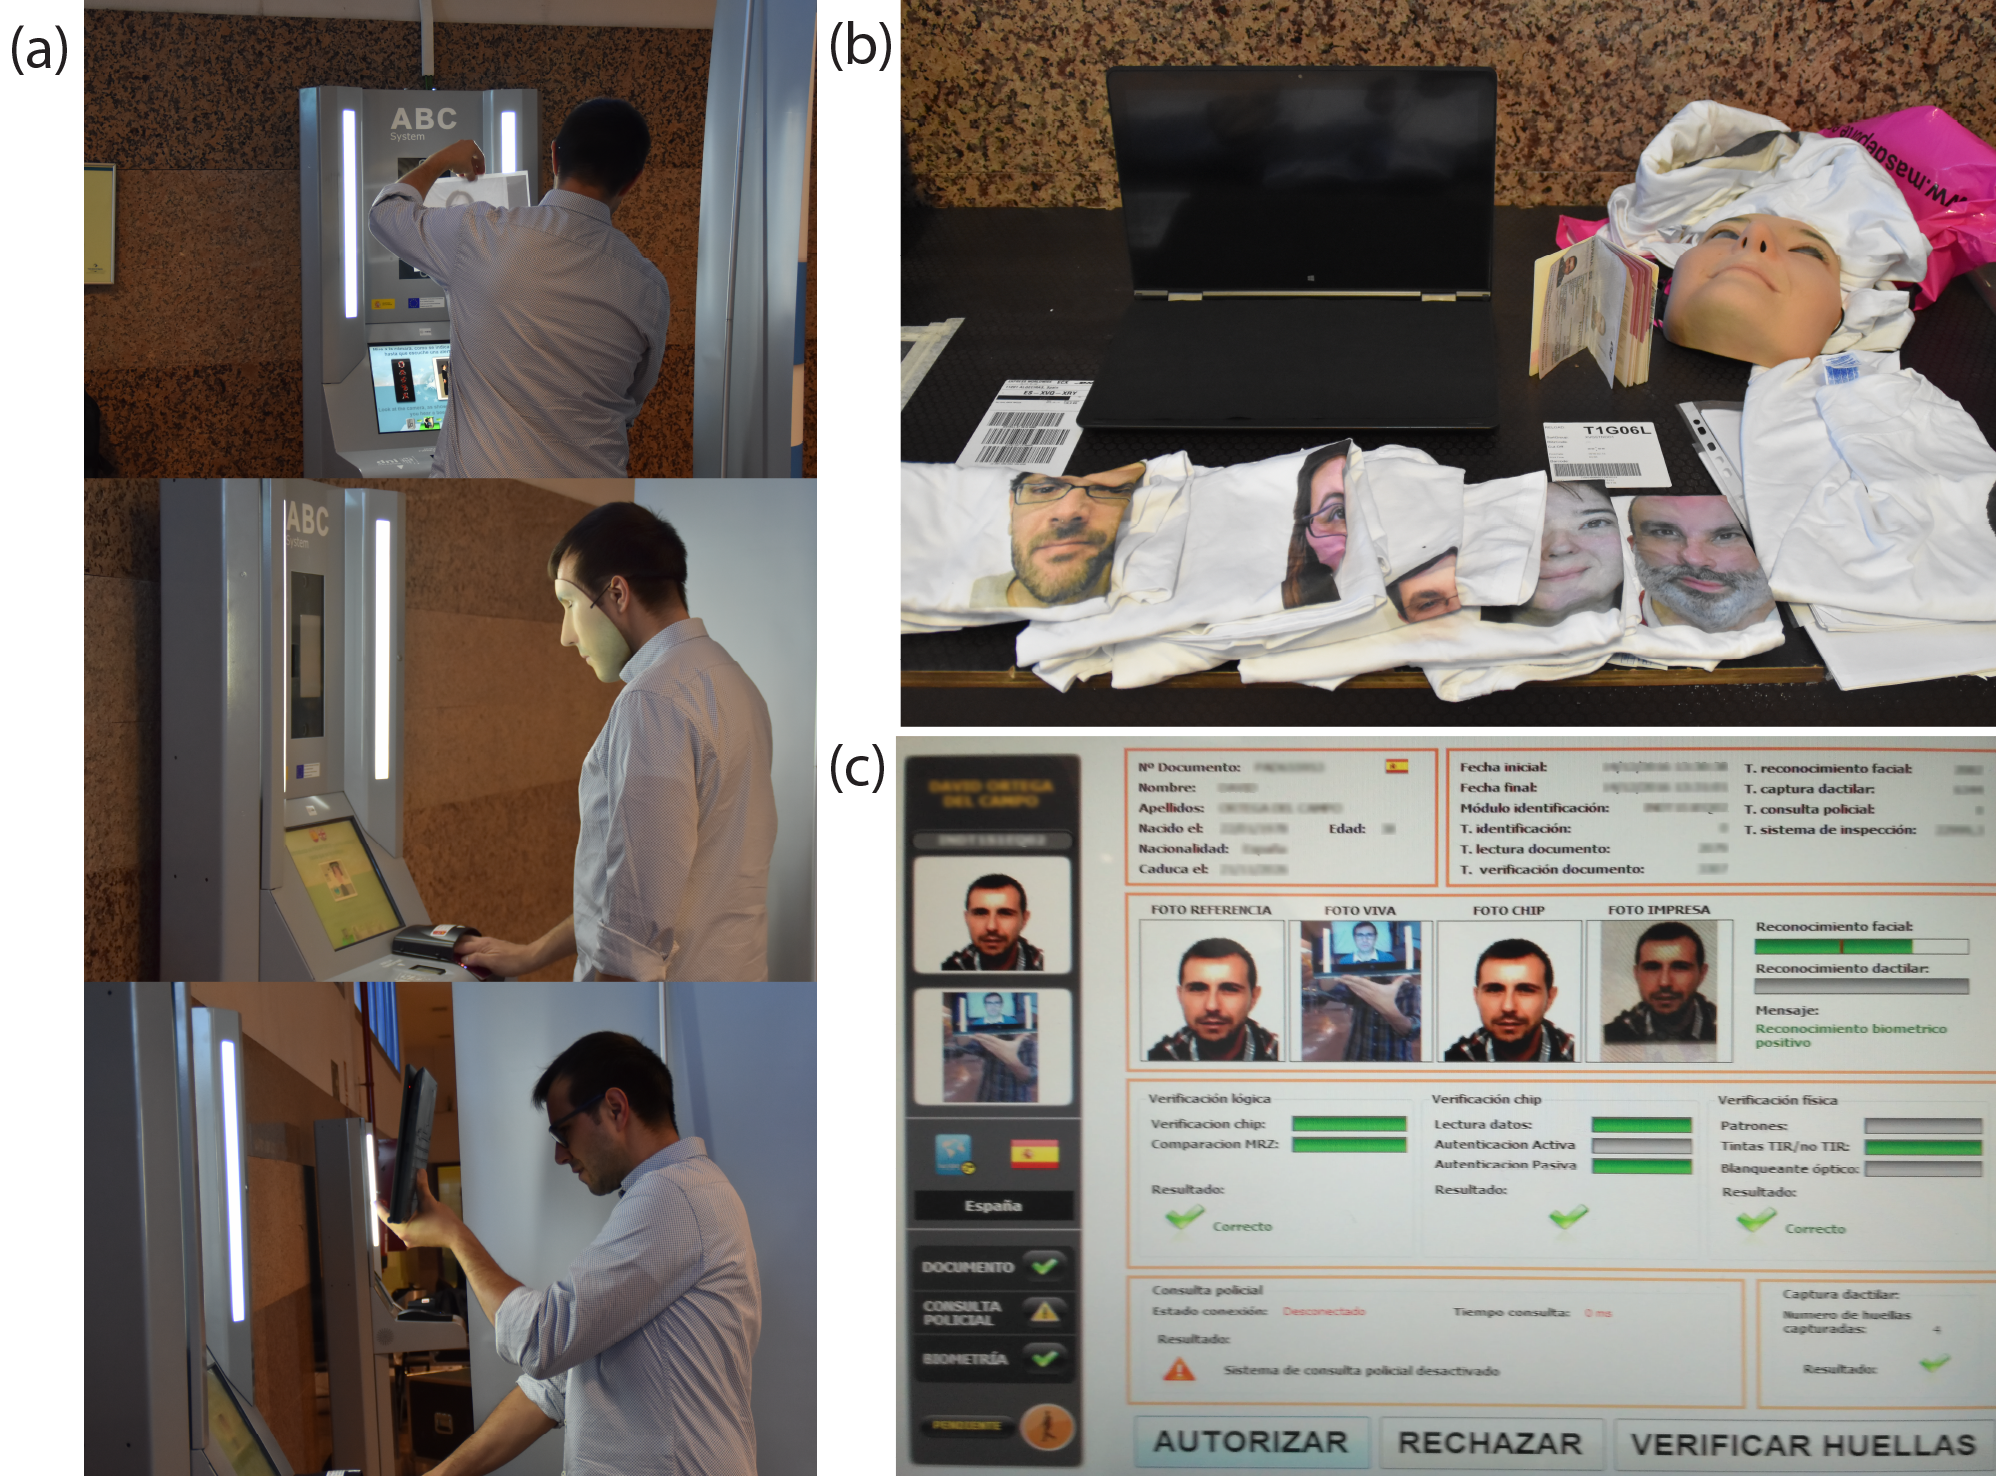
\includegraphics[width=1\linewidth]{ch-sistemasABC/images/ch-BBDDs/CAPTURA_FRAV_ABC.png}
    \caption{Imágenes de la adquisición de la base de datos \Gls{FRAV-ABC}: (a) Presentación de ataques en el dispositivo. (b) \Glspl{PAI} de los distintos ataques. (c) Pantalla de traza de los dispositivos.}
    \label{fig:AdquisicionFRAVABC}
\end{figure}

En esta sección se describe la base de datos \gls{FRAV-ABC-Attack}\footnote{La base de datos \Gls{FRAV-ABC-Attack} se capturó en las mismas circunstancias que \Gls{FRAV-ABC}.}, compuesta por 300 sujetos (160 mujeres y 140 hombres), ya incluidos \gls{FRAV-ABC} y cuyos datos fueron capturados también un dispositivo \GLS{ABC} en un cruce de fronteras real (ver Fig. \ref{fig:AdquisicionFRAVABC}). Pero, en este caso se incluyeron: la imagen \gls{chip} y varias \gls{vivo}: un  \gls{vivo bona-fide} y 5 \gls{vivo ataque}. Las imágenes \gls{chip} con formato \GLS{RGB} de $300\times300$ píxeles y todas las imágenes \gls{vivo}, también \GLS{RGB} de $300\times300$ píxeles. En suma, 300 imágenes \gls{chip}, 300 \gls{vivo bona-fide} y 1500 \gls{vivo ataque}.

\medskip
\textbf{\textit{<<vivo bona-fide>>}}

Las imágenes \gls{vivo bona-fide} son imágenes capturadas \textit{in situ} en un cruce de fronteras real por un dispositivo \GLS{ABC} operativo con una presentación del sujeto genuino.

\medskip
\textbf{\textit{<<vivo ataque>>}}

Las imágenes \gls{vivo ataque} son imágenes capturadas \textit{in situ} en un cruce de fronteras real por un dispositivo \GLS{ABC} operativo, con presentaciones con algún \GLS{PAI} de los contemplados: Máscara $3$D, fotografía, máscara de cartón, vídeo y camiseta (Ver Fig. \ref{fig:SAMPLES-FRAV-ABC-ATTACK}).
\medskip

Los ataques contemplados para la realización de esta base de datos son similares a los que se incluyen en \Gls{FRAV-Attack} (ver Sección \ref{subsec:FRAV-ABC-ATTACK}) pero además se ha añadido un nuevo \GLS{PAI}, el ataque con camiseta, que consiste en llevar una prenda de vestir con la fotografía serigrafiada del viajero genuino, este \GLS{PAI} permite engañar al sistema si la detección facial encuentra la cara estampada antes que la del impostor (ver Fig. \ref{fig:SAMPLES-FRAV-ABC-ATTACK} (g)).

%%%%%%%%%%%%%%%%%%%%% FRAV ABC ATTACK DOS PASOS SEGREGADOS %%%%%%%%%%%%%%%%%%%%%%% 
\subsection{FRAV-ABC-Attack \textit{<<Segregated Two Step>>}}\label{subsec:FRAV-ABC-ATTACK-DOS_PASOS}

\begin{figure}[ht]
     \centering
     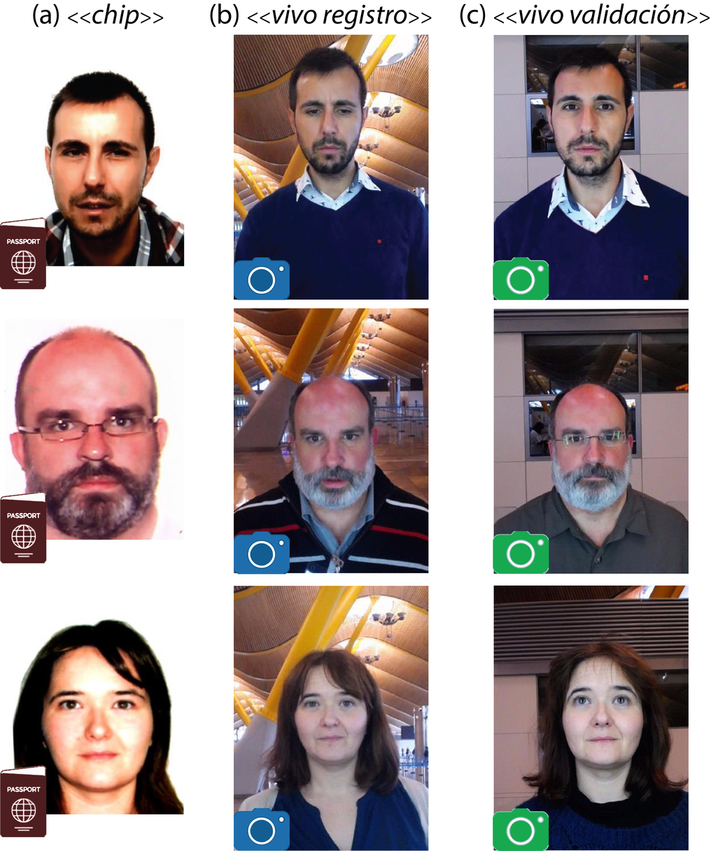
\includegraphics[width=0.6\textwidth]{ch-sistemasABC/images/ch-BBDDs/VERIFICACION_DAVID_ENRIQUE_CRISITNA_DOS_PASOS.png}
     \caption{Imágenes \gls{FRAV-ABC-Attack} en un sistema \GLS{ABC} \textit{<<Segregated Two Step>>} con doble verificación: (a) Imagen \gls{chip}. (b) Imagen \gls{vivo registro} en \GLS{RTP}  y (c) Imagen \gls{vivo validacion} en \GLS{EES}.}
     \label{fig:Imagenes_ABC_Attack_dosPasos}
\end{figure}

Los datos de $100$ sujetos de la base de datos de \Gls{FRAV-ABC-Attack} se adquirieron con sistemas \GLS{ABC} \textit{<<Segregated Two Step>>} lo que implica dos capturas biométricas, una en la etapa de \GLS{RTP} y otra en \GLS{EES} (ver apartado: \ref{subsec:ArquitecturaLogicaABC}). De cada sujeto se incluyeron su imagen \gls{chip}, \gls{vivo registro} capturada en la tapa \GLS{RTP} y \gls{vivo validacion} capturada en la etapa \GLS{EES} (ver Fig. \ref{fig:Imagenes_ABC_Attack_dosPasos}).

\medskip
\textbf{\gls{vivo registro}}

Las imágenes \gls{vivo registro} son imágenes capturadas en la etapa de \GLS{RTP} \textit{in situ} por un dispositivo \gls{e-kiosk} de un cruce de fronteras real.

\medskip
\textbf{\gls{vivo validacion}}

Las imágenes \gls{vivo validacion} son imágenes capturadas en la etapa de \GLS{EES} \textit{in situ} por un dispositivo \gls{e-gate} de un cruce de fronteras real.
\medskip

En cada una de las etapas también se simularon ataques con lo que para cada etapa se obtuvieron capturas: \gls{vivo registro bona-fide}, \gls{vivo registro ataque} y \gls{vivo validacion bona-fide} y \gls{vivo validacion ataque}.

%%%%%%%%%%%%% BASESD DE ATOS PARA SISTEMAS ABC ONTHEFLY %%%%%%%%%%%%%%%%%%%% 
\section{Bases de datos para sistemas ABC \textit{OnTheFly}}\label{sec:BBDD-OnTheFly}

En estas sección se describen dos bases de datos diseñadas para sistemas \GLS{ABC} con captura dinámica: \Gls{FRAV-OnTheFly} y \Gls{FRAV-ABC-OnTheFly}. Se puede encontrar mas información sobre este tipo de sistemas en la Sección \ref{sec:tiposABC}. Todas las capturas incluidas en estas bases de datos son vídeos. En el caso de \Gls{FRAV-OnTheFly}, vídeos capturados en un laboratorio en condiciones controladas, con sujetos que simulan el comportamiento de viajeros frente a un sistemas \GLS{ABC} con captura dinámica, mientras que en \Gls{FRAV-ABC-OnTheFly} los vídeos se capturaron en un verdadero sistema \GLS{ABC} con captura dinámica, en un cruce de fronteras real.

Las dos bases datos se construyeron para una investigación sobre ataques de presentación en sistemas \GLS{ABC} con captura dinámica \cite{ortega2020dynamic}, cuyo objetivo consistía en proponer un método para la detección de este tipo de ataques. Para ello, además de los vídeos con presentaciones \gls{bona-fide} de cada sujeto, se simularon una serie de vídeos con ataques de presentación, usando \GLS{PAI} similares a los incluidos en \Gls{FRAV-ABC-Attack} (ver apartado \ref{subsec:FRAV-ABC-ATTACK}). Los trabajos realizados en estas investigaciones y los resultados obtenidos se exponen en detalle en el Capítulo \ref{ch:ABC_OnTheFly}.

%%%%%%%%%%% BASES DE ATOS PARA SISTEMAS ABC ONTHEFLY  CAPTURADA EN LABORATORIO %%%%%%%%%%%%%%%% 
\subsection{\textit{FRAV-OnTheFly}: Escenario controlado}\label{subsec:BBDD-FRAV-OnTheFly}

\begin{figure}[ht]
     \centering
     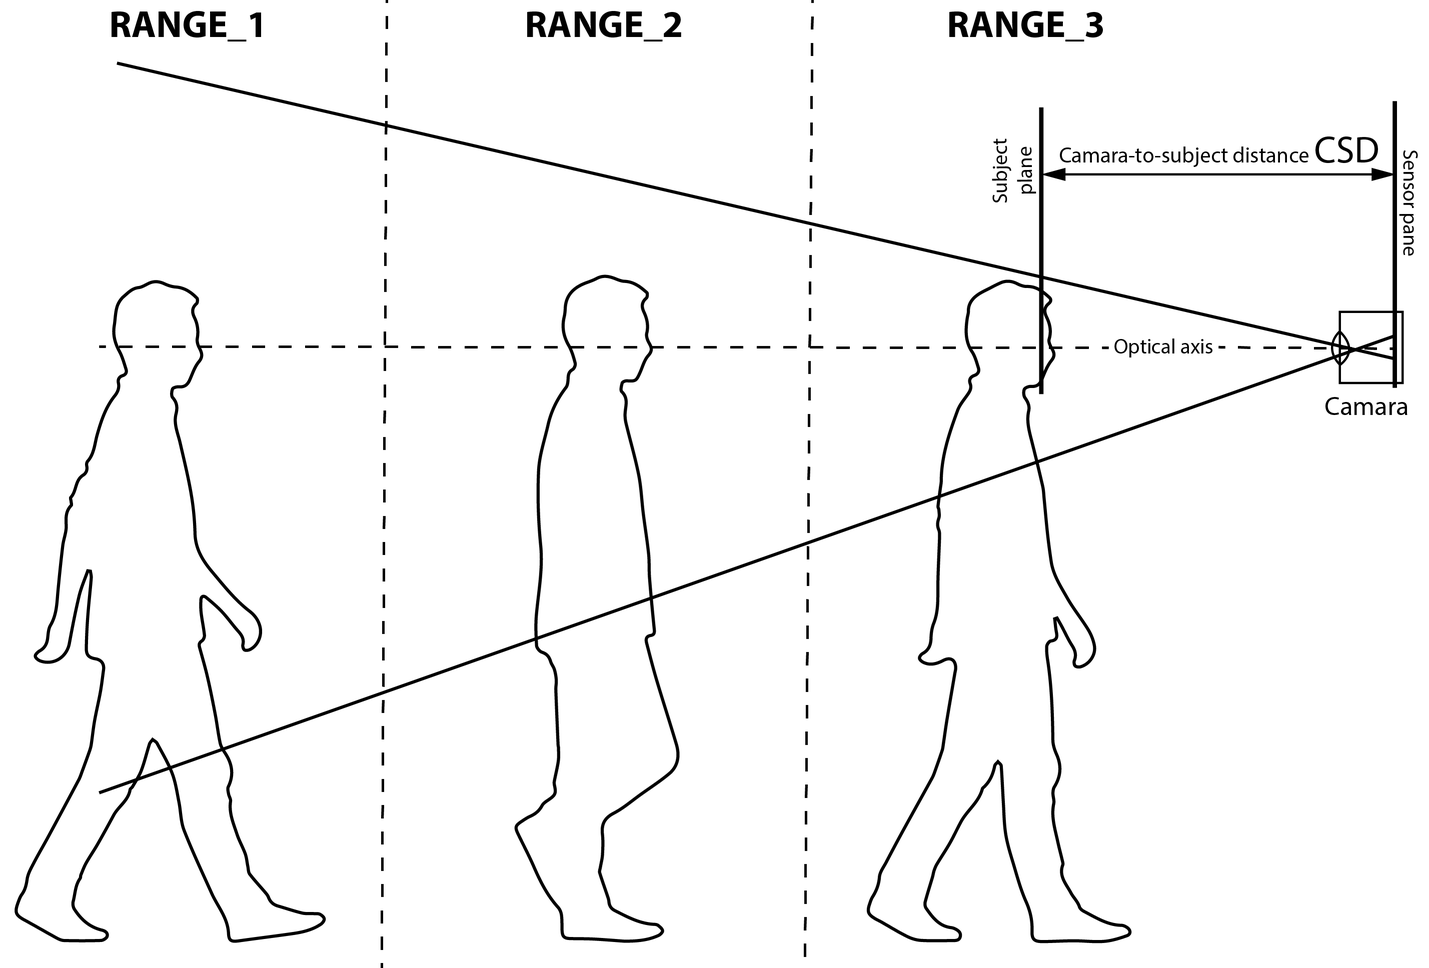
\includegraphics[width=0.8\textwidth]{ch-sistemasABC/images/ch-BBDDs/CAPTURA_ONTHEFLY.png}
     \caption{Esquema del proceso de captura de \textit{FRAV-OnTheFly}.}
     \label{fig:EsquemaCapturaFRAVABCOmTheFly}
\end{figure}

La base de datos de \Gls{FRAV-OnTheFly} incluye 178 sujetos y contiene 1068 vídeos. Estos vídeos tienen 25 fps (fotogramas por segundo) y una resolución de $1,920\times1,080$ píxeles (ver Fig. \ref{fig:fravattackonthefly}).

La base de datos consta de 82 mujeres y 96 hombres. Las edades oscilan entre los 18 y los 67 años, con aproximadamente el $70$ por ciento de los sujetos en el rango de edad de $18$ a $28$ años. La selección de los individuos para la base de datos se hizo de acuerdo con las estadísticas de cruce de fronteras que imitan su distribución. Se construyó una base de datos con estudiantes voluntarios, profesores y personal universitario. Todos los sujetos mantienen su privacidad y, de acuerdo con las normas de protección de datos, se requirió el consentimiento informado de todos los sujetos. La adquisición de buena fe se llevó a cabo durante una semana y después, tras construir los \GLS{PAI} de todos los sujetos, la captura de los vídeos de ataque se realizó en dos días. 

Los vídeos para la base de datos se capturaron en el laboratorio en condiciones de iluminación controlada. Estos vídeos se grabaron con una cámara de alta resolución Sony\textsuperscript{\textregistered}$\alpha6000$ (ver apartado \ref{sec:BBDD-FRAV-Attack}). 

Se enseñó a los sujetos a simular el comportamiento de los viajeros en un cruce de frontera con un sistema \GLS{ABC} de captura dinámica. Así, los sujetos caminan desde 3 metros de la cámara hasta medio metro (ver Fig. \ref{fig:EsquemaCapturaFRAVABCOmTheFly}). Se grabaron seis vídeos diferentes siguiendo este procedimiento (uno por cada tipo de ataque y uno para el \gls{bona-fide}). 

\begin{table}
\centering
\begin{tabular}{|c|c|c|}
\hline
\textbf{Rango} & \textbf{Tamaño imagen} & \textbf{Distancia} \\ \hline
\textbf{Fuera de Rango} & $50\times50$ px & -- \\ \hline
\textbf{Rango-$1$} & $\geq{}$ $50\times50$ px -- \textless{} $150\times150$ px & $\geq{}$ $2$m \\ \hline
\textbf{Rango-$2$} & $\geq{}$ $150\times150$ px -- \textless{} $250\times250$ px & \textless{} $2$m $\geq{}$ $1$m \\ \hline
\textbf{Rango-$3$} & $\geq{}$ $250\times250$ px & \textless{} $1$m \\ \hline
\end{tabular}
\caption{Rangos en los que se clasifican las caras en \Gls{FRAV-OnTheFly} y en \Gls{FRAV-ABC-OnTheFly} atendiendo a la distancia del sujeto al dispositivo, calculada mediante al tamaño de la región de cara detectada.}
\label{tab:facesranges_FRAV_OnTheFly}
\end{table}

Una vez que se capturaron todos los vídeos se realizó un proceso de recuperación de las imágenes faciales. Cada fotograma de los vídeos fue procesado con el algoritmo \textit{\gls{Viola-Jones}} \cite{viola2004robust} para detectar caras. Atendiendo al tamaño de la región detectada, las caras se etiquetaron en un determinado rango. Se consideraron tres rangos (ver Tabla \ref{tab:facesranges_FRAV_OnTheFly}). 

\medskip
\textbf{Rango-1}

Caras detectadas a más de 2 metros del dispositivo, cuya región tiene un tamaño mayor o igual que $50\times50$ píxeles y menor que $150\times150$ píxeles.

\medskip
\textbf{Rango-2}

Caras detectadas a una distancia entre 1 metro y 2 metros del dispositivo, cuya región tiene un tamaño mayor o igual que $150\times150$ píxeles y menor que $250\times250$ píxeles.

\medskip
\textbf{Rango-3}

Caras detectadas a menos de 1 metro del dispositivo, cuya región tiene un tamaño mayor que $250\times250$ píxeles.

\medskip
\textbf{Fuera de rango}

Las caras detectadas con regiones menores a $50\times50$ píxeles se consideraron caras fuera de rango que no pueden ser procesadas. 

\medskip

\begin{table}[ht!]
    \centering
    \begin{tabular}{|l|c|c|c|c|c|c|} \hline
    \multicolumn{7}{|c|}{\rule{0pt}{25pt} \shortstack{\textbf{FRAV-OnTheFly} \\ ($178$ subjects - $1,068$ videos - $120,425$ faces)}} \\ \hline 
    \small{\textbf{Rango}} & \small{\textbf{Bona fide}} & \small{\textbf{Photo}} & \small{\textbf{Video}} & \small{\textbf{Mask}} & \small{\textbf{Mask w/e}} & \small{\textbf{$3$D Mask}} \\ \hline 
    \small{\textbf{Rango-$1$}} & $8,799$ & $8,525$ & $8,330$ & $8,203$ & $8,329$ & $412$ \\ \hline
    \small{\textbf{Rango-$2$}} & $8,837$ & $8,730$ & $8,750$ & $8,335$ & $8,420$ & $441$ \\ \hline
    \small{\textbf{Rango-$3$}} & $8,843$ & $8,603$ & $8,603$ & $8,208$ & $8,225$ & $435$ \\ \hline
    \end{tabular}
    \caption{Número de caras detectadas en los vídeos de la base de datos \gls{FRAV-OnTheFly}.}
    \label{tab:faces-FRAV-OnTheFly}
\end{table}

Finalmente, la información de la base de datos es almacenada para los tres rangos definidos (Ver Tabla \ref{tab:faces-FRAV-OnTheFly}). Nótese que hay diferentes cantidades de fotogramas con caras porque a veces una cara no puede ser detectada en todos los fotogramas de la secuencia.


%%%%%%%%%%%%%%%%%%% FRAV ABC ONTHEFLAY CAPTURADA EN ABC %%%%%%%%%%%%%%%
\subsection{\textit{FRAV-ABC-OnTheFly}: ABC en frontera real}\label{subsec:BBDD-FRAV-ABC-OnTheFly}

\begin{figure}[h!]
    \centering
    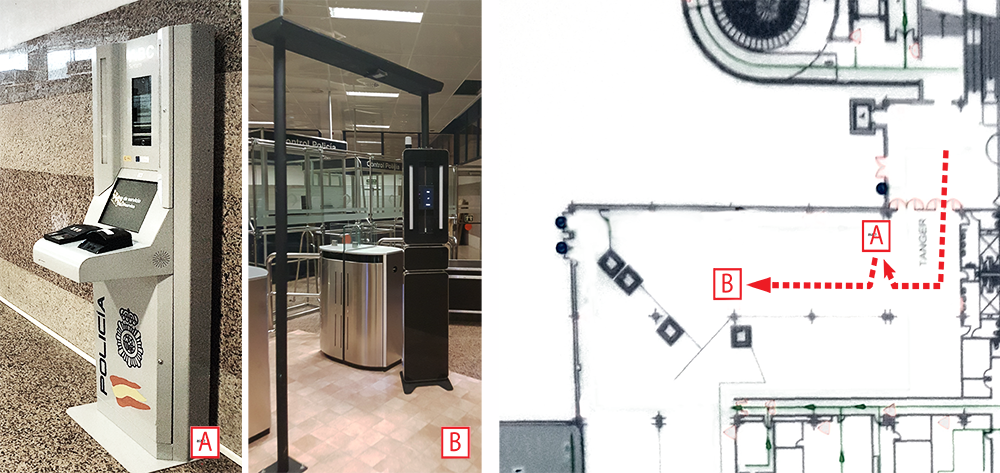
\includegraphics[width=1\textwidth]{ch-sistemasABC/images/ch-onthefly/realDevices.png}
    \caption{Escenario real con los dispositivos \gls{e-kiosk} y \gls{e-gate}.}
    \label{fig:realdevices}
\end{figure}

La base de datos \Gls{FRAV-ABC-OnTheFly} se capturó en un sistema \GLS{ABC} \textit{<<Segregated Two Step>>}\footnote{\Gls{FRAV-ABC-OnTheFly} se capturó durante la implantación de los sistemas \GLS{ABC} piloto del Proyecto Europeo \GLS{ABC4EU} \cite{ABC4EUOnline} en el puerto marítimo de Algeciras (España). Este puerto es una frontera del área de \textit{\Gls{Schengen}}, siendo un importante punto de entrada y salida para viajeros del norte de África.} con dos dispositivos: un \gls{e-kiosk} donde se realizaba la etapa \GLS{RTP} y un \gls{e-gate} para la etapa de \GLS{EES} (ver Fig. \ref{fig:realdevices}). Los viajeros se registraban en el \gls{e-kiosk}, mostrando su documentación y posteriormente se dirigían a la \gls{e-gate} para completar el cruce. La captura en el \gls{e-kiosk} se realizaba de forma estática, el viajero debe detenerse ante el dispositivo para que su identidad se verifique con la almacenada en sus documentos. Sin embargo en la \gls{e-gate} la captura es dinámica y la verificación con alguna de identidades registradas se realiza mientras que el viajero se aproxima a la puerta.
% (la arquitectura \Gls{FlyPAD} Para esta captura dinámica es para la que se propone  presentada en el capitulo \ref{ch:ABC_OnTheFly}.

\Gls{FRAV-ABC-OnTheFly} incluye 10 sujetos, 5 mujeres y 5 hombres, de edades comprendidas entre los 22 y los 56 años. Al igual que en \Gls{FRAV-OnTheFly} se grabaron vídeos de $1920\times1080$ píxeles a 25 fps, Con cada sujeto se grabó un vídeo \gls{bona-fide} aproximándose a la puerta y 5 vídeos de ataque con diferentes \GLS{PAI}.

\begin{table}[ht!]
\centering
\begin{tabular}{|l|c|c|c|c|c|c|} \hline
\multicolumn{7}{|c|}{\rule{0pt}{25pt} \shortstack{\textbf{FRAV-ABC-OnTheFly} \\ ($10$ subjects - $60$ videos - $7,200$ faces)}} \\ \hline
\small{\textbf{Range}} & \small{\textbf{Bona fide}} & \small{\textbf{Photo}} & \small{\textbf{Video}} & \small{\textbf{Mask}} & \small{\textbf{Mask w/e}} & \small{\textbf{$3$D Mask}} \\ \hline 
\small{\textbf{Range-$1$}} & $440$ & $402$ & $318$ & $350$ & $347$ & $408$ \\ \hline
\small{\textbf{Range-$2$}} & $481$ & $411$ & $421$ & $417$ & $428$ & $423$ \\ \hline
\small{\textbf{Range-$3$}} & $403$ & $383$ & $370$ & $403$ & $408$ & $387$ \\ \hline
\end{tabular}
\caption{Número de caras detectadas en los vídeos de la base de datos \Gls{FRAV-ABC-OnTheFly}.}
\label{tab:faces-FRAV-ABC-OnTheFly}
\end{table}

Una vez que se capturaron todos los vídeos se realizó un proceso de recuperación de las imágenes faciales y una clasificación por rangos, atendiendo a la  distancia del sujeto al dispositivo. Los rangos considerados son los mismos que en \Gls{FRAV-OnTheFly} (ver apartado \ref{subsec:BBDD-FRAV-OnTheFly}) y el número total de caras detectadas en cada rango se pude ver en la tabla \ref{tab:faces-FRAV-ABC-OnTheFly}.

\begin{landscape}
\begin{figure}
    \centering
    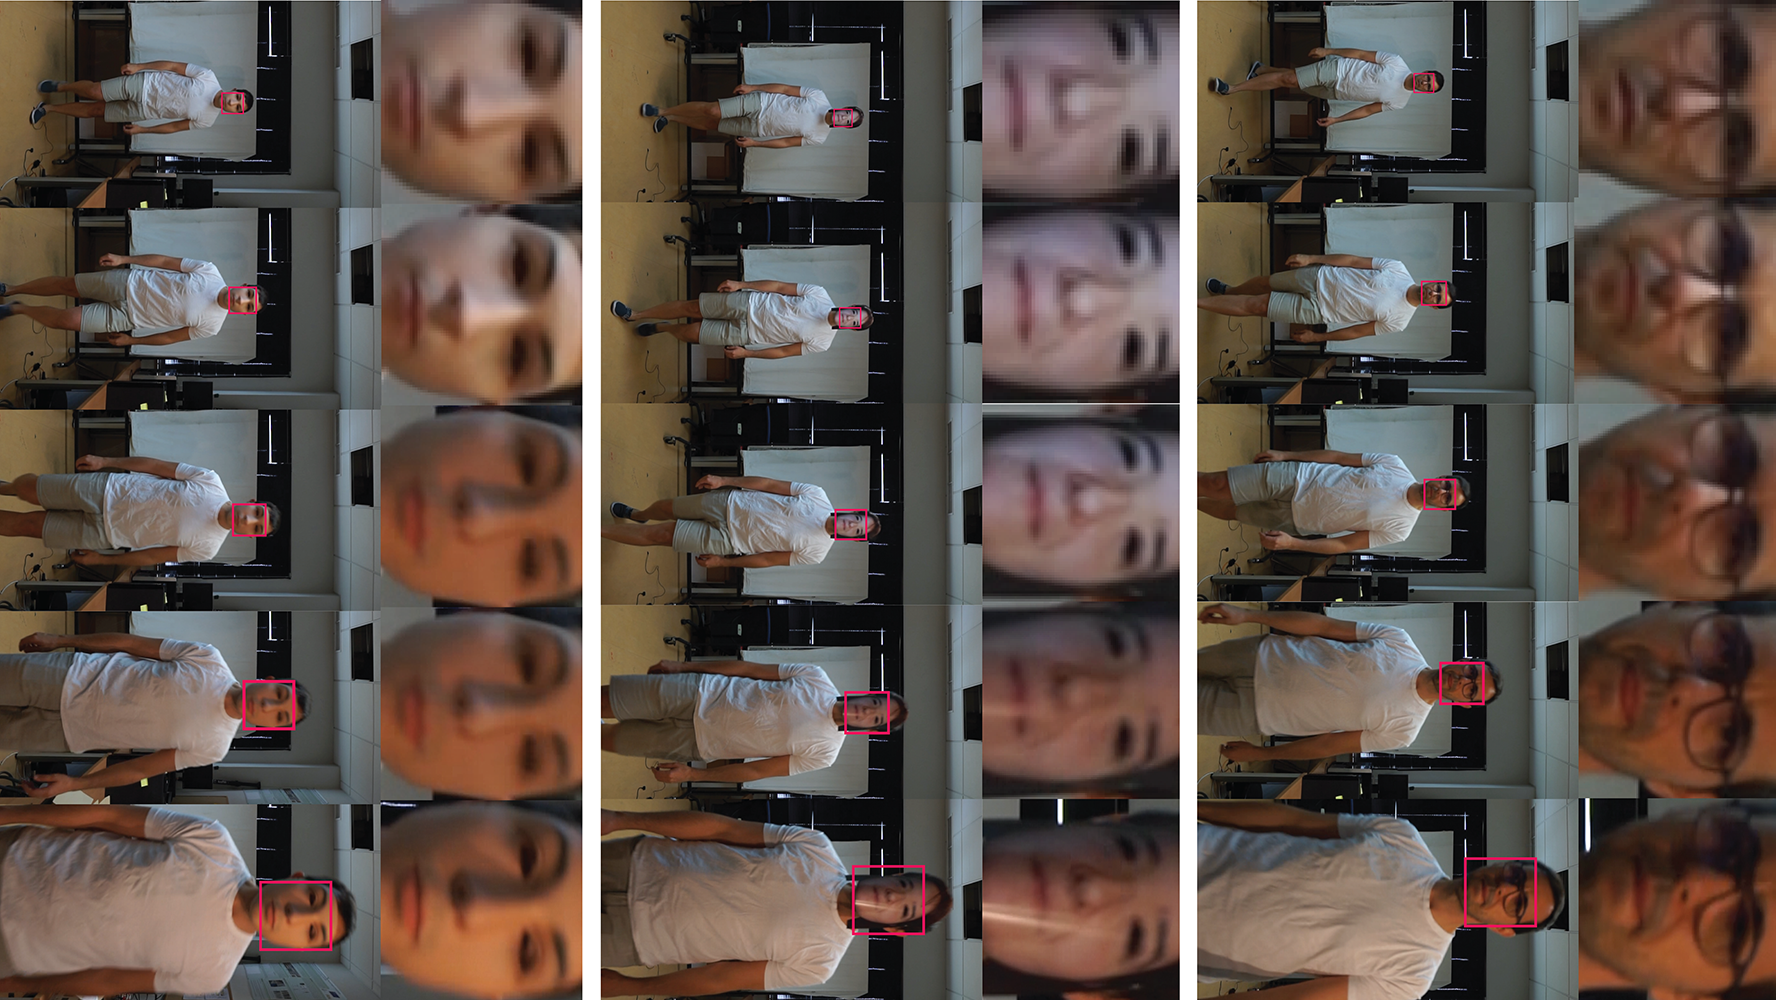
\includegraphics[scale=1.5]{ch-sistemasABC/images/ch-BBDDs/FRAVAttackOnTheFly.png}
    \caption{Capturas de vídeos almacenados en la base de datos \Gls{FRAV-OnTheFly}.}
    \label{fig:fravattackonthefly}
\end{figure}
\end{landscape}

%%%%%%%%%%%%%% FRAV ABC MORPHING  %%%%%%%%%%%%%%%%%%%%%%%%%%%%%%%%%%%%%%% 
\section{Bases de datos para MAD}\label{sec:BBDD_Morphing}

En esta sección se presenta la base de datos \Gls{FRAV-Morphing} construida para investigaciones sobre ataques de presentación de tipo \gls{morphing} \Gls{FRAV-Morphing}. Los ataques se han creado fusionando las imágenes \gls{chip} de los sujetos de la base de datos \Gls{FRAV-ABC} (ver sección \ref{sec:BBDD-ABC}), construyendo imágenes \gls{chip morphing} mediante un método automático descrito en el apartado \ref{subsec:MorphingMethods}.

de la publicación \cite{ortega2020border}, descrita en detalle en el Capítulo \ref{ch:morphing}.  

En el apartado \ref{subsec:FRAV-Morphing} se explica cómo se ha estructurado la base de datos en varios subconjuntos para entrenamiento, validación y test, evitando mezclar sujetos entre conjuntos.

En el apartado \ref{subsec:BBDD_MorphingPrintScan} se explica como se imprimieron y se escanearon para acercar los datos a la problemática real que se produce en la construye un documento de viaje.

%%%%%%%%% METODO MORPHING  %%%%%%%%%%%
\subsection{Método \textit{morphing}}\label{subsec:MorphingMethods}

\begin{figure}[ht]
     \centering
     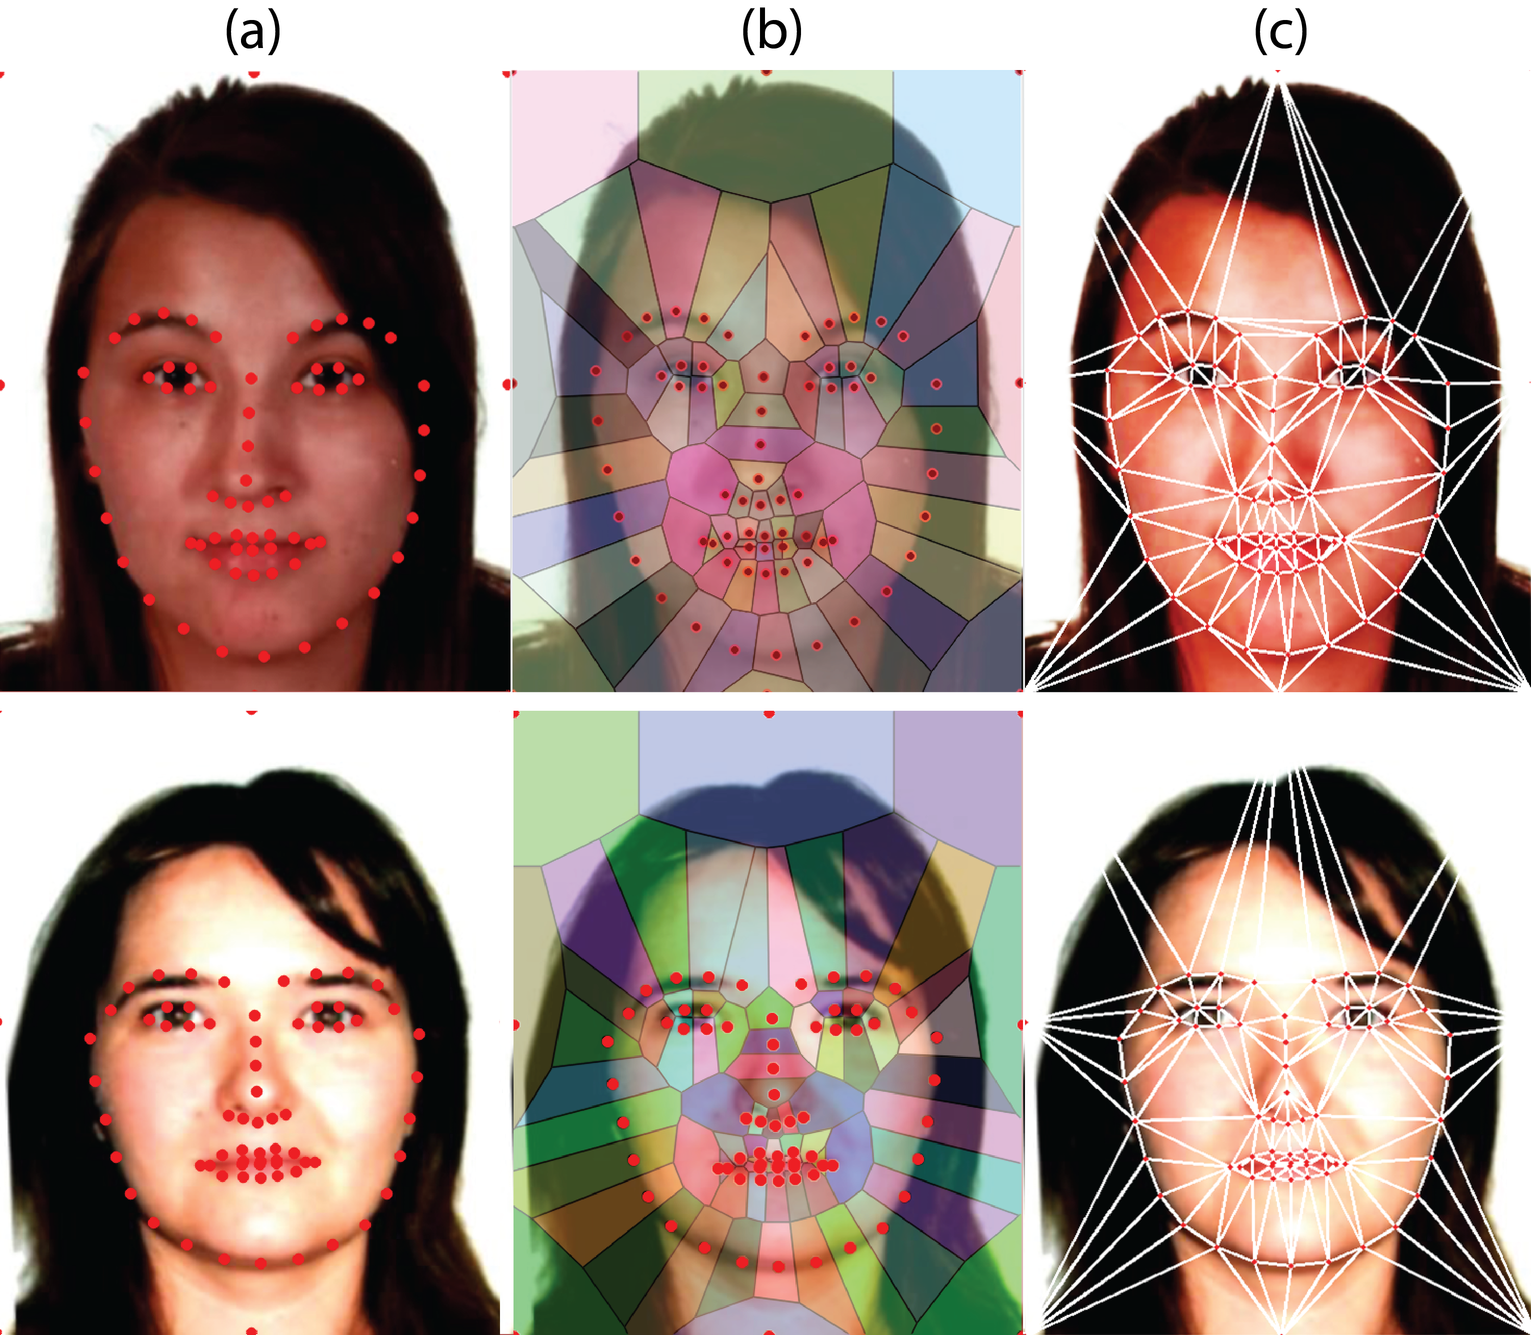
\includegraphics[width=0.8\textwidth]{ch-sistemasABC/images/ch-morphing/TRIANGULACION-CHIP-BEA-CRISTINA.png}
     \caption{(a) \textit{Detección de Landmark faciales}, (b) \textit{Calculo de Delaunay} y (c) \textit{Triangulación Voronoi}.}
     \label{fig:LandmarckDVTriangualtion}
\end{figure}

\begin{figure}[ht]
     \centering
     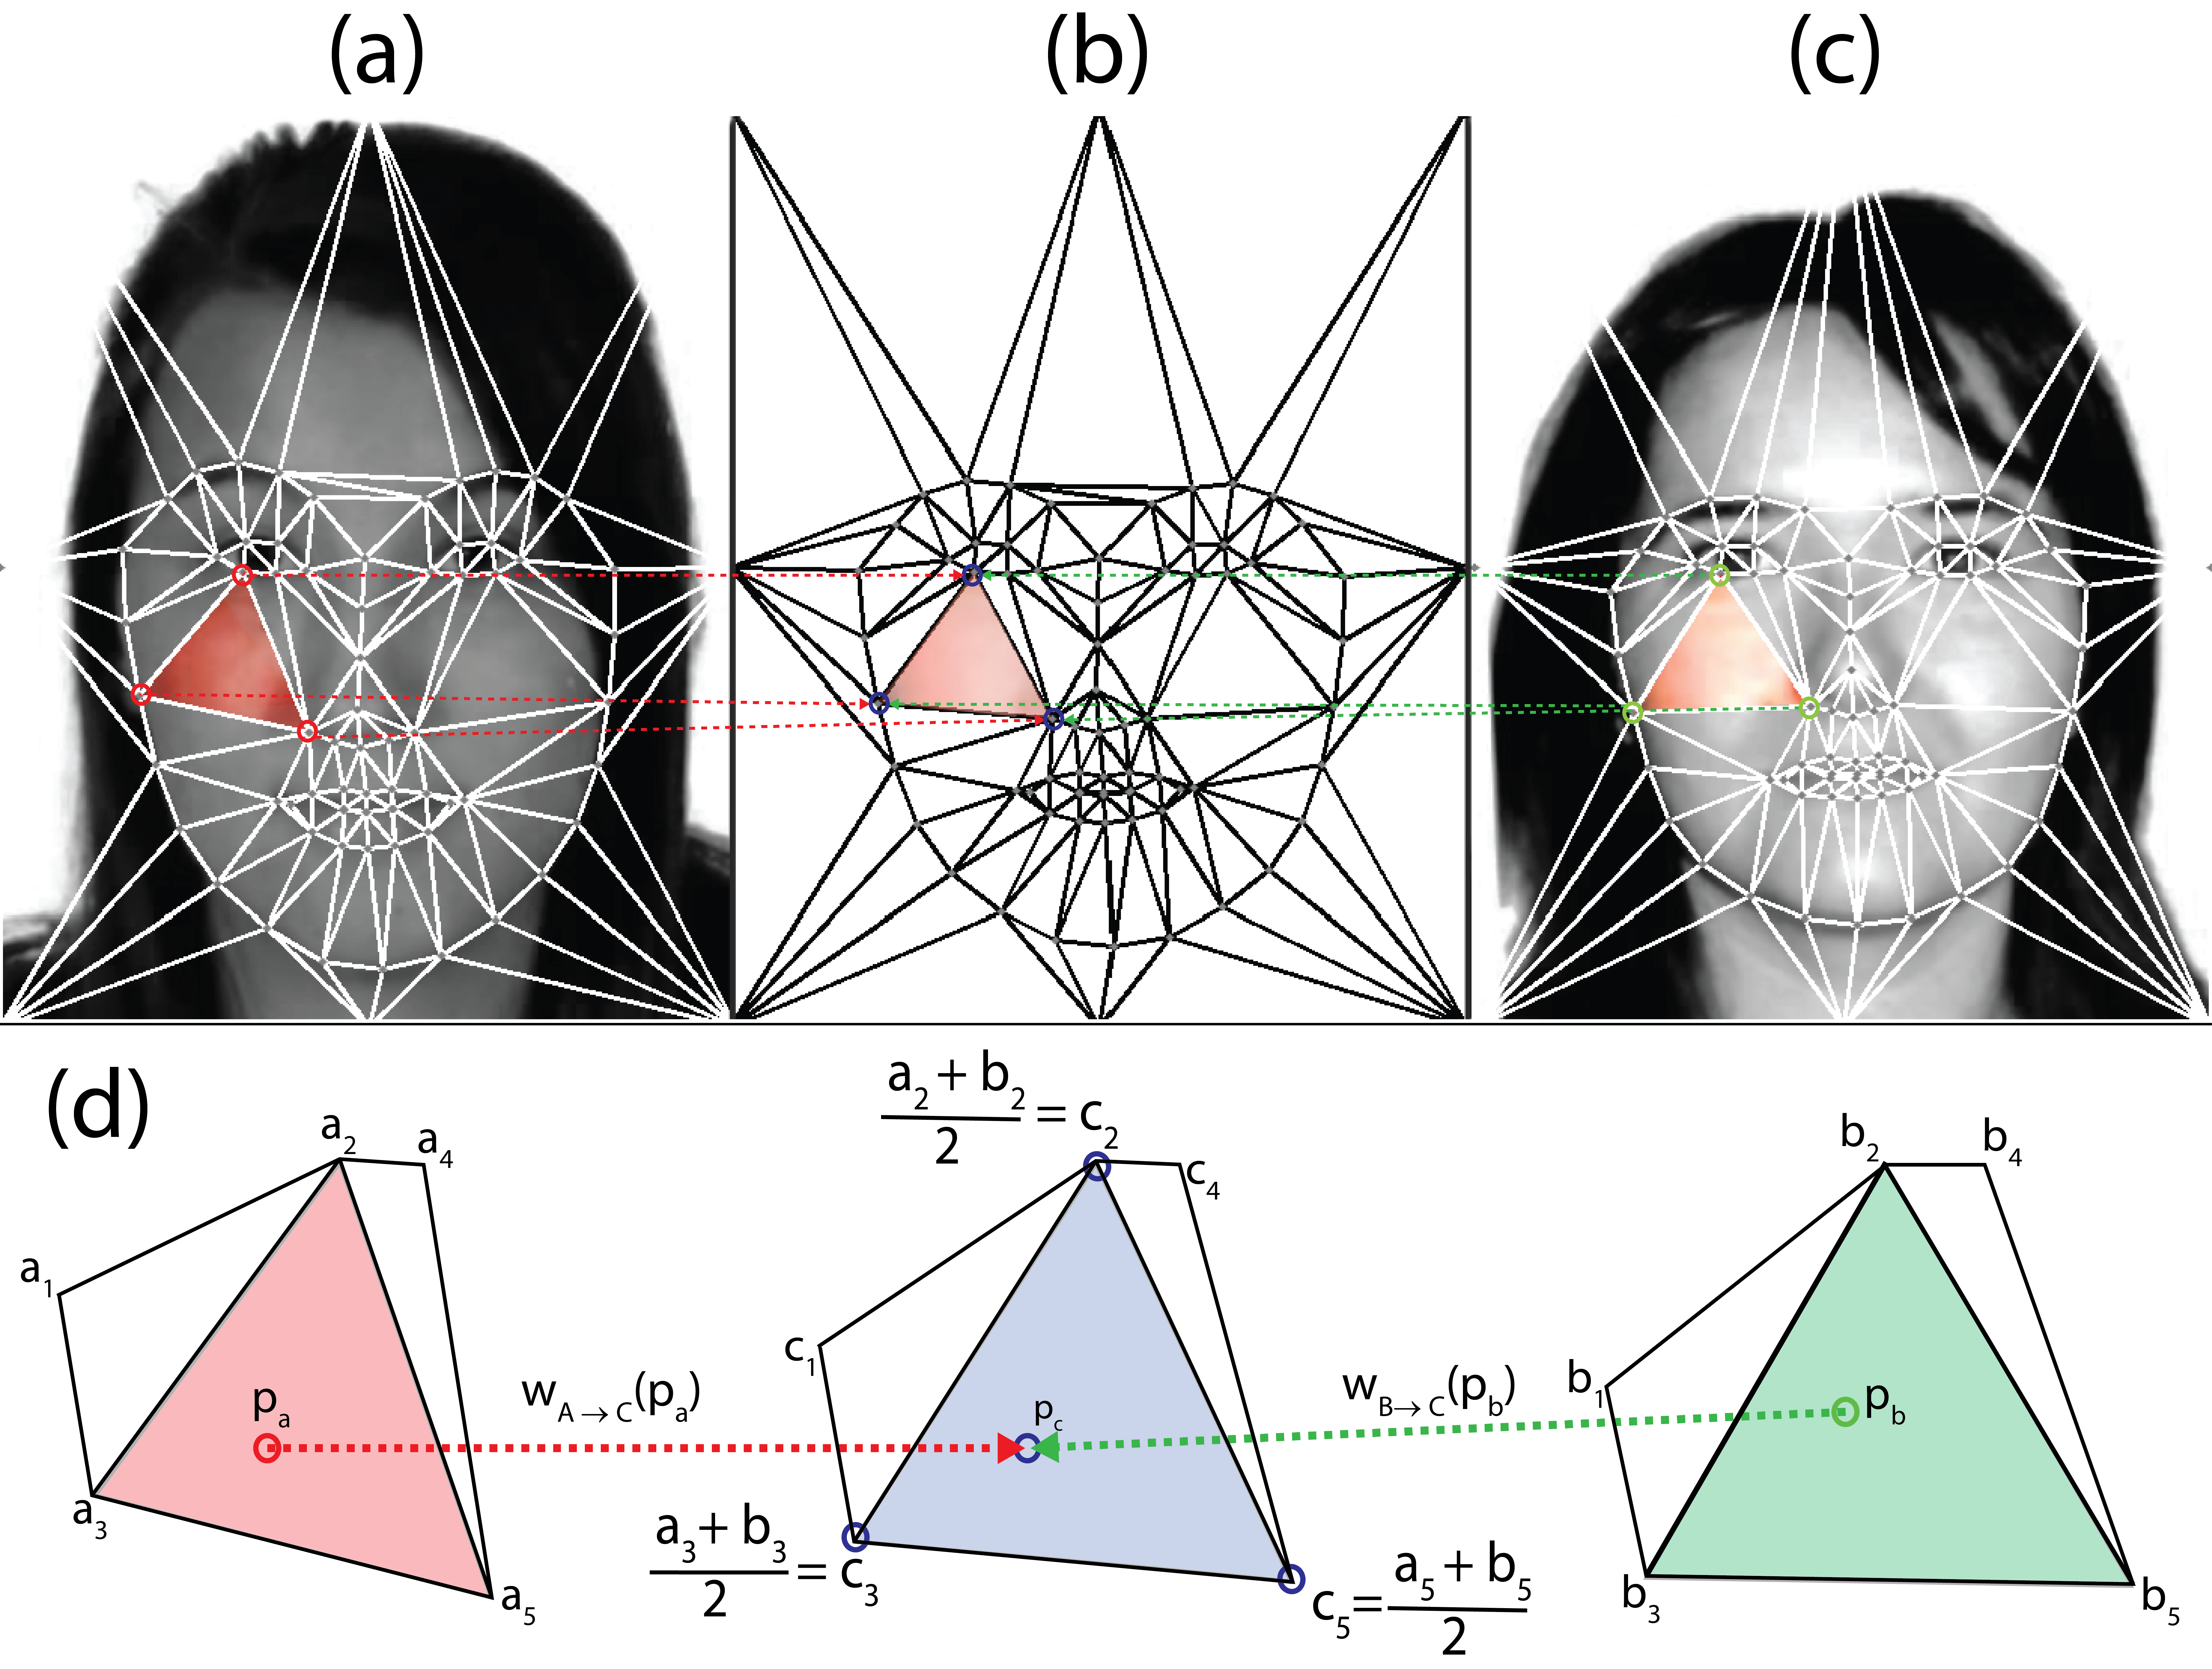
\includegraphics[width=0.8\textwidth]{ch-sistemasABC/images/ch-morphing/TriangulacionFusion_CristinaBea_COMPACTA.png}
     \caption{Warping the morphed target image and blending each source triangle that contained pixels.}
     \label{fig:Triangulación}
\end{figure}

\begin{figure}[ht]
     \centering
     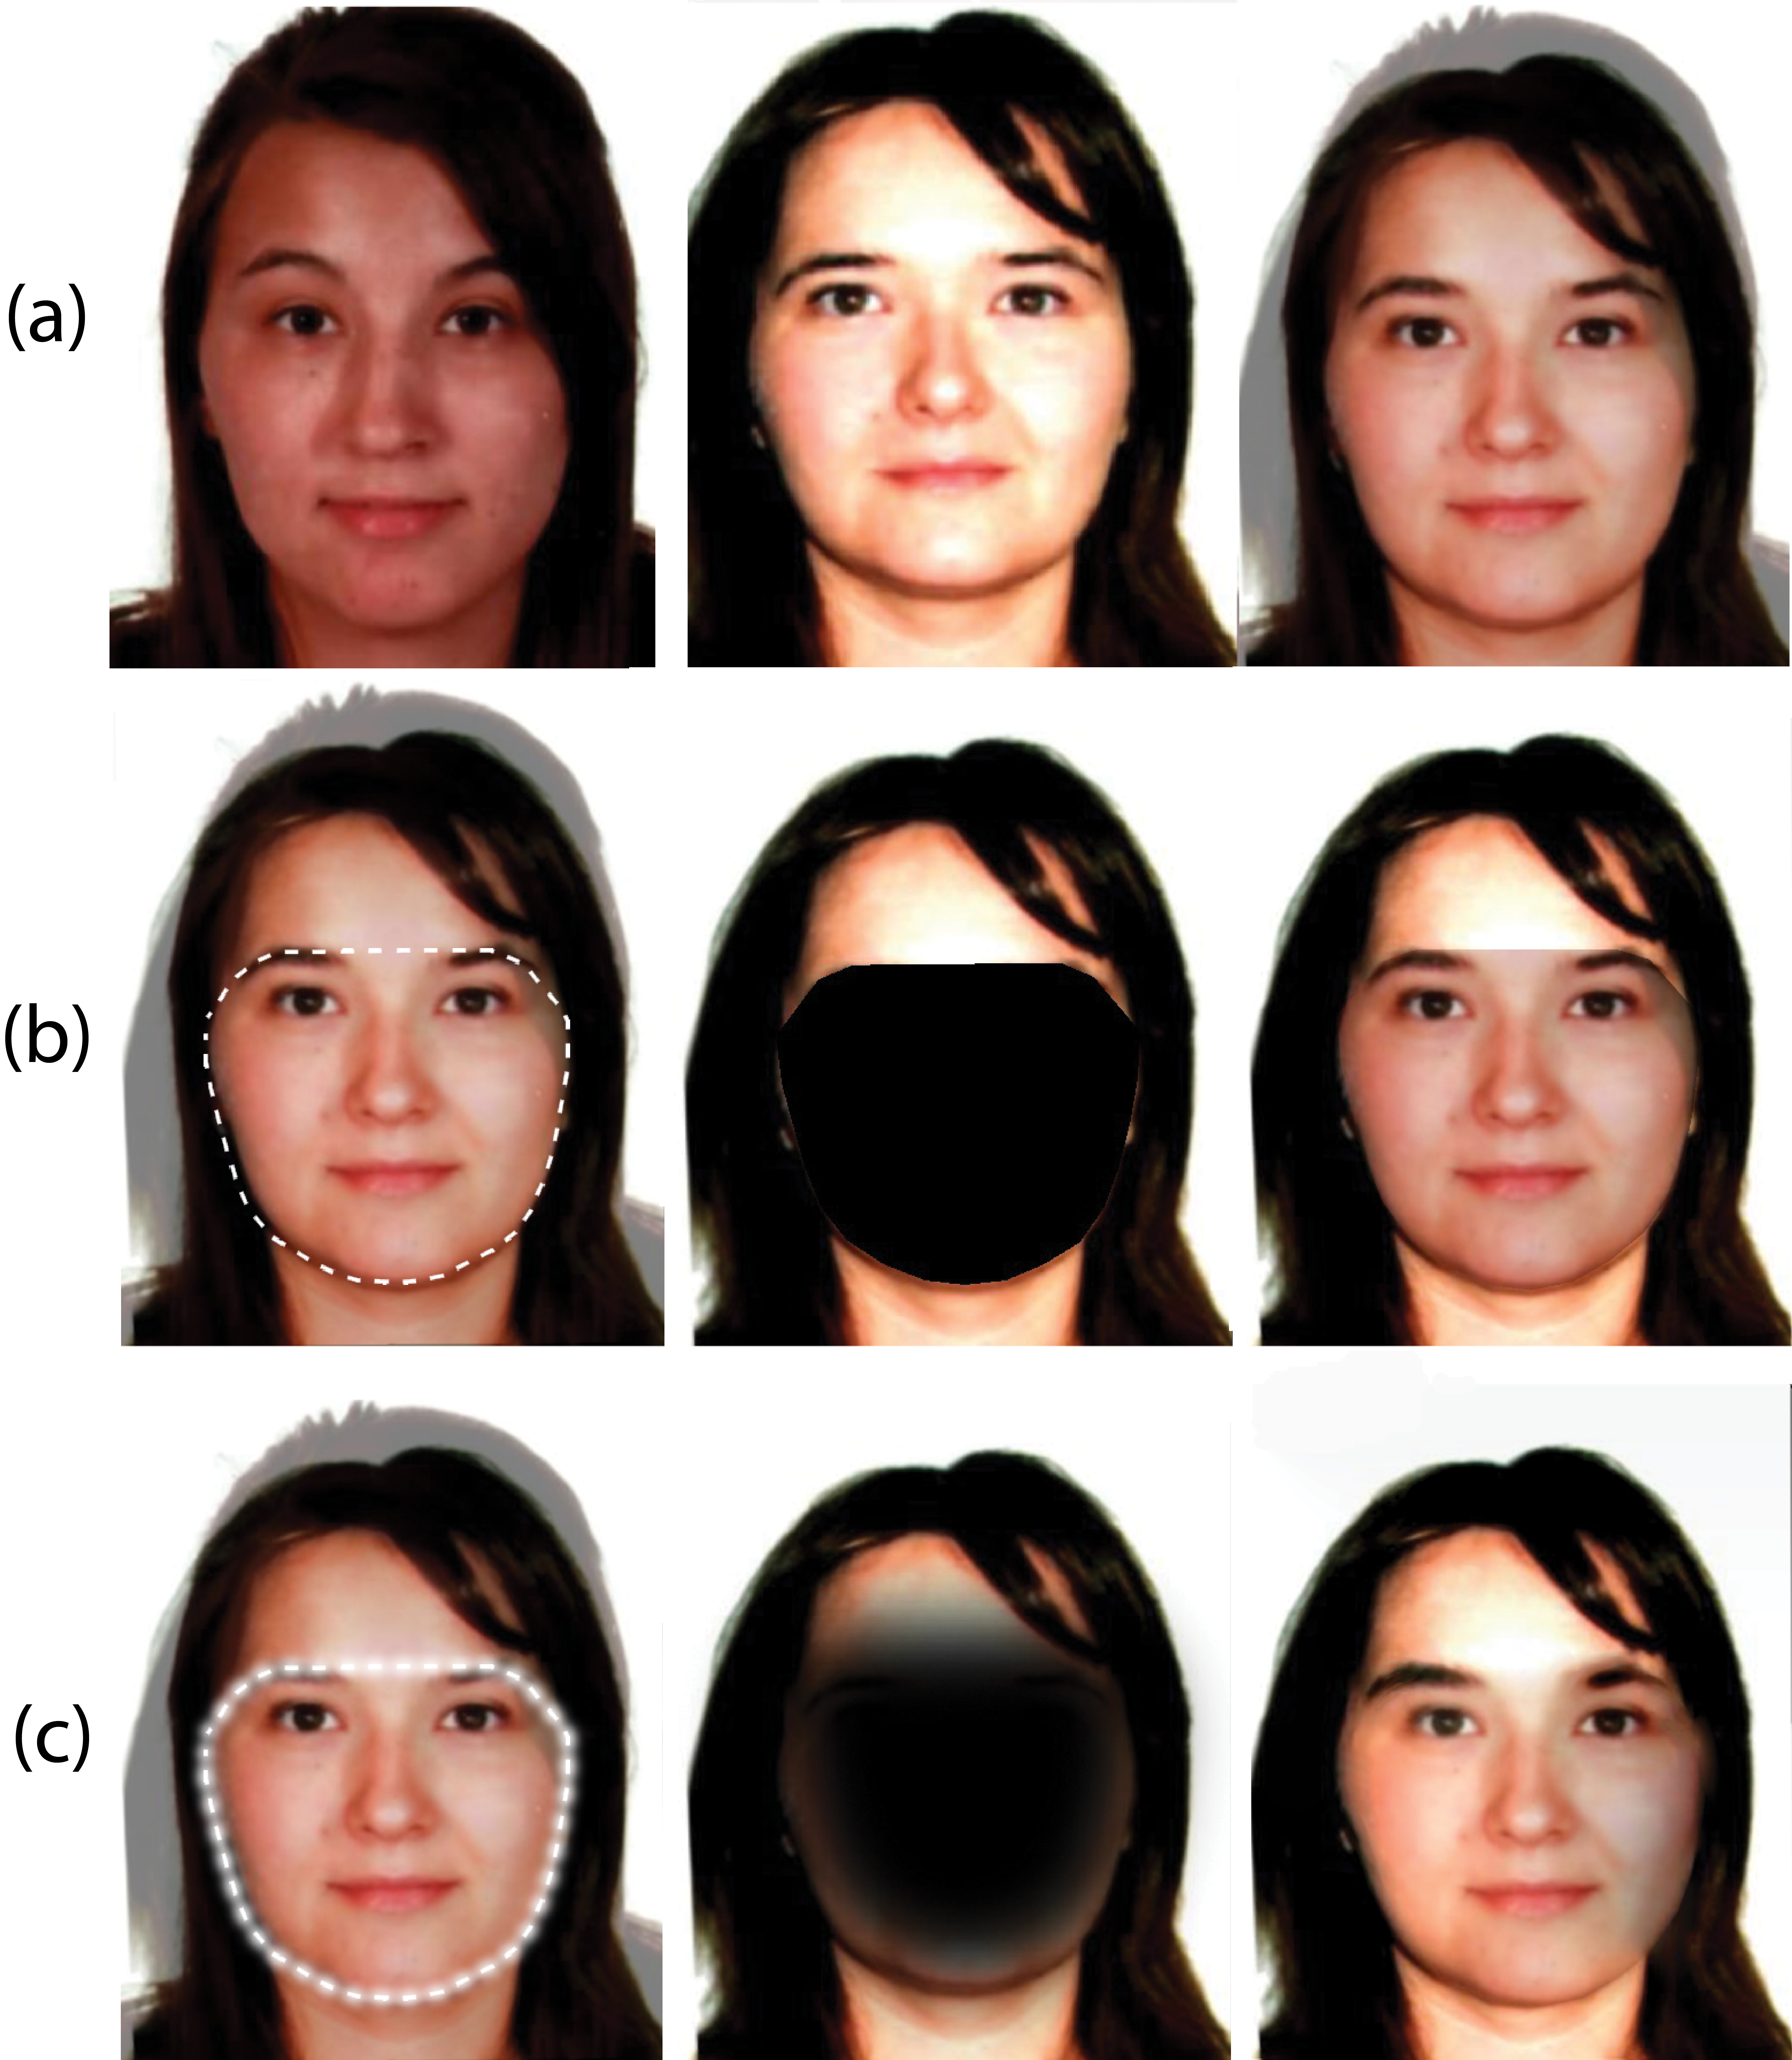
\includegraphics[width=0.8\textwidth]{ch-sistemasABC/images/ch-morphing/MorphingEnhanceMask_COMPACTA.png}
     \caption{(a)Average image, (b) Clipping and replacing the  face region and (c) the fuzzy mask to enhance the result and cropping source image.}
     \label{fig:Enhancement}
\end{figure}

% \begin{figure}[ht]
%     \centering
%     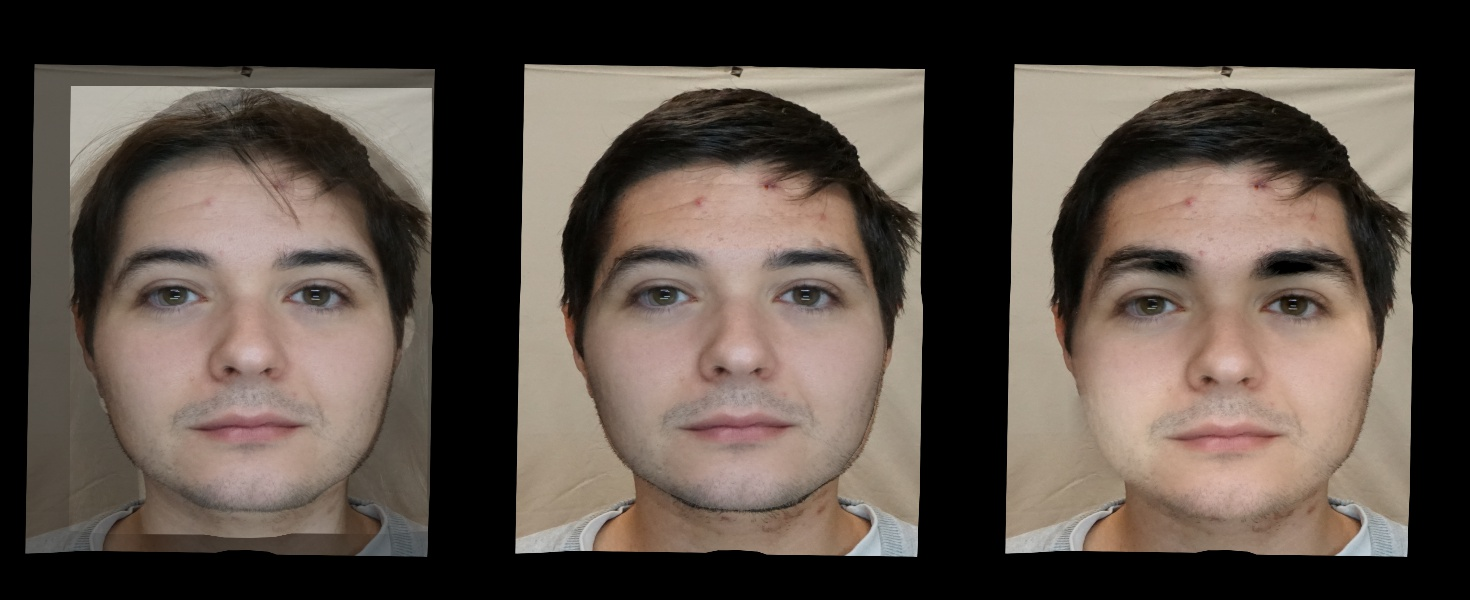
\includegraphics[width=\textwidth]{ch-sistemasABC/images/ch-morphing/old/coreccion_mophings.jpg}
%     \caption{Corrección del \textit{morphing}.}
%     \label{fig:morphing_correccion}
% \end{figure}

% \begin{figure}[ht]
%     \centering
%     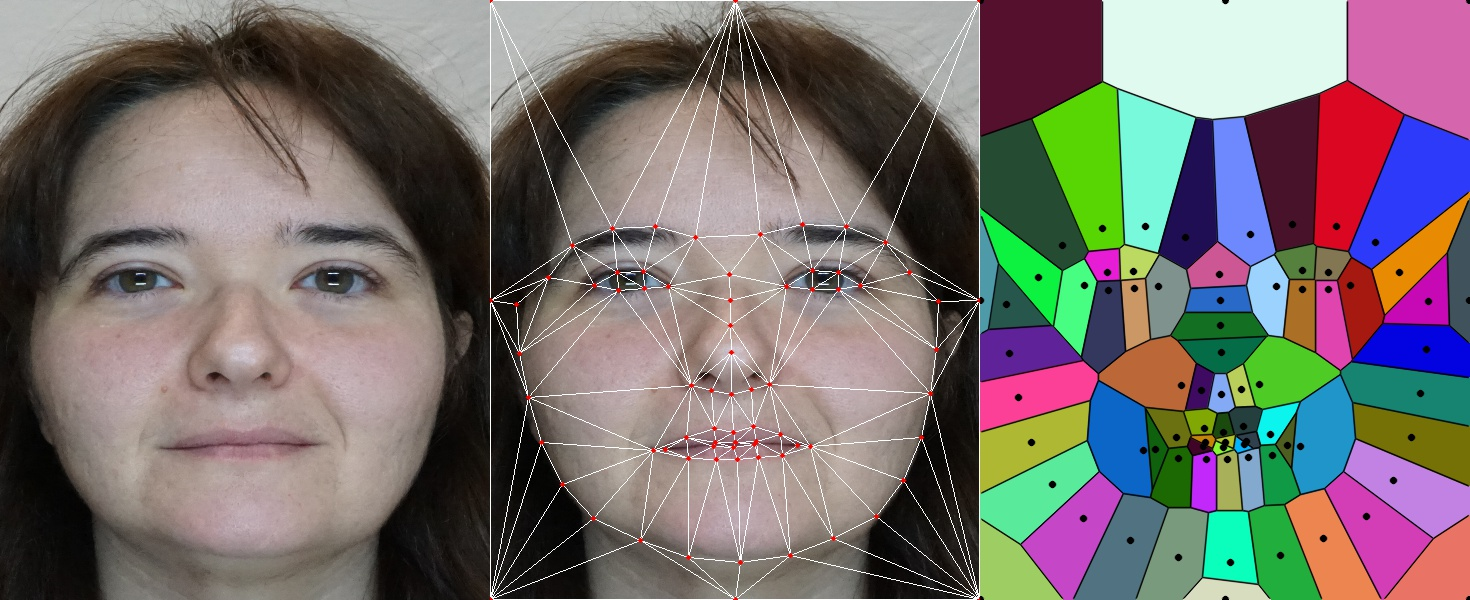
\includegraphics[width=\textwidth]{ch-sistemasABC/images/ch-morphing/old/delaunay-voronoy.jpg}
%     \caption{Triangulación Delaunay-Voronoi.}
%     \label{fig:morphing_delaunay_voronoi}
% \end{figure}

% \begin{figure}[ht]
%     \centering
%     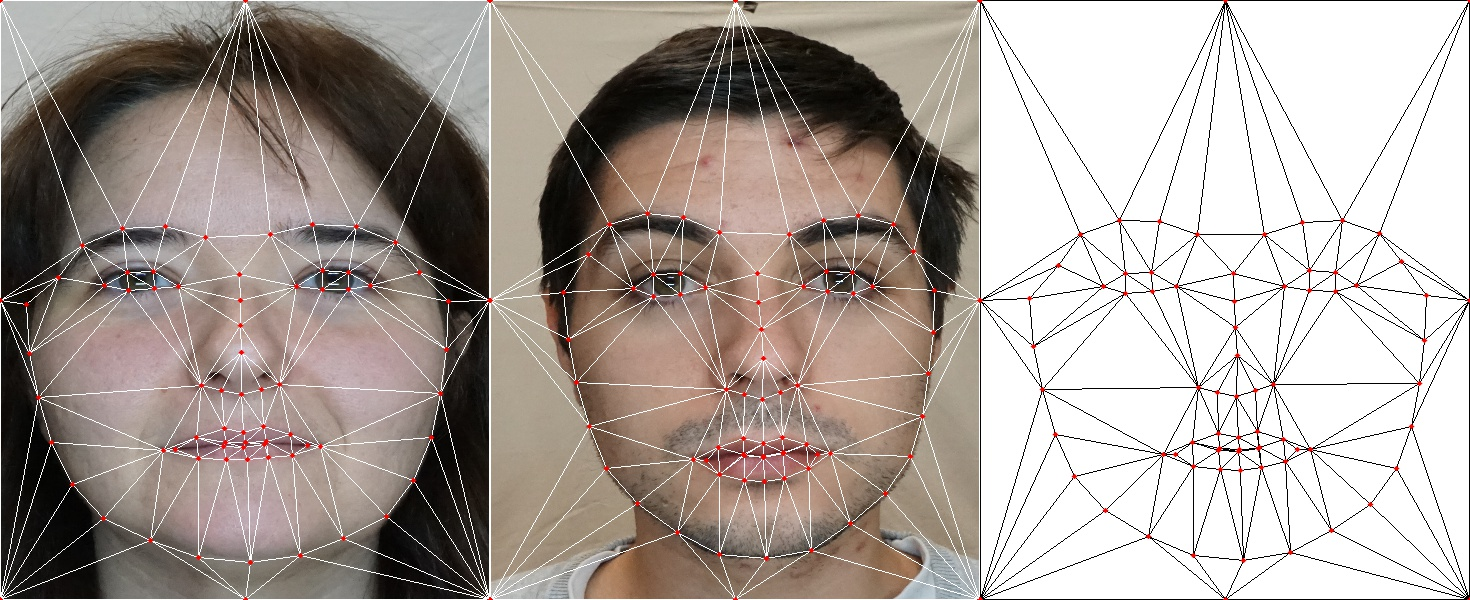
\includegraphics[width=\textwidth]{ch-sistemasABC/images/ch-morphing/old/triangulationImage.jpg}
%     \caption{Triangulación del \textit{morphing}.}
%     \label{fig:morphing_triangulacion}
% \end{figure}

Actualmente, es posible encontrar herramientas de software comercial para la construcción de imágenes \gls{morphing} de alta calidad (\cite{FantaMorphOnline}, \cite{MorpheusOnline}, \cite{MorphThingOnline}, \cite{NukeOnline}, \cite{SilhouetteFXOnline}, \cite{GimpOnline}, \cite{FaceMorpherOnline}, \cite{WinMorphOnline}), pero todas ellas, en mayor o menor medida, requieren procesos manuales. Cuando se necesita un gran número de imágenes hay que buscar un proceso automático. El algoritmo presentado en \cite{ferrara2017face}, \cite{scherhag2019face} permite esta automatización del proceso. 

Esta sección describe el proceso \gls{morphing} empleado para la construcción de los distintos conjuntos de la base de datos \Gls{FRAV-Morphing}. El proceso propuesto se divide en dos etapas: Una primera de fusión de las identidades que mezcla las dos imágenes y una segunda de corrección y mejora del resultado final que consigue una imagen más realista.

\medskip
\textbf{Fusión de identidades}
\medskip

La construcción del \textit{morphing} se realiza en tres de pasos: Detección de punto de referencia, triangulación y mezcla.

\begin{enumerate}

\item 
Dadas las dos imágenes a fusionar en cada una de ellas se detectan $76$ puntos de referencia que posteriormente ayudarán en su triangulación: $68$ \textit{\glspl{landmark}} faciales. detectados mediante el algoritmo propuesto por \textit{Kazemi} y \textit{Sullivan} \cite{kazemi2014one} (implementado en \Gls{Dlib} \cite{dlibOnline}) y ocho puntos que forma parte del borde de la imagen (las esquinas y los puntos medios de cada lado)

\item 
con los puntos de referencia detectados se realiza una triangulación de las imágenes con el algoritmo \textit{Delaunay-Voronoi} (\GLS{DVT} \cite{lokhande2013morphing}) (ver Figura \ref{fig:LandmarckDVTriangualtion}, que consiste en unión de los puntos de referencia (con camino \textit{Delaunay} mínimo) de los puntos de regiones de \textit{Voronoi} colindantes (ver Fig. \ref{fig:LandmarckDVTriangualtion} (b) y (c)). Como la triangulación se realiza en las dos imágenes a fusionar cada triangulo en una imagen  tiene un triángulo homólogo en la otra imagen (Fig. \ref{fig:Triangulación}).

\item 
Cada par de triángulos homólogos se deforman y se mezclan componiendo una nueva imagen que es la imagen promedio, este proceso de deformación y mezcla se conoce como \textit{warping} \cite{wu2011face}, \cite{jassim2018automatic}, \cite{hildebrandt2017benchmarking} (ver Fig. \ref{fig:Triangulación}). Los vértices de cada nuevo triangulo son los puntos medios de los vértices correspondientes de los triángulos a deformar y lo \textit{pixels} contenidos se fusionan atendiendo a un factor de mezcla (habitualmente al $50$\%). 

\end{enumerate}

\medskip
\textbf{Corrección y mejora de la fusión}
\medskip


La imagen promedio tiene demasiados artefactos (\textit{ghost artifacts}), especialmente en las regiones periféricas y resulta muy detectable visualmente como ataque de presentación (ver Fig. \ref{fig:Enhancement} (a)). Para mejorar el resultado final de la fusión y obtener una apariencia más realista se puede retocar la imagen manualmente \cite{ferrara2014magic} o aplicar algunos ajustes automáticos \cite{ferrara2017face}:

\begin{enumerate}
\item 
Una mejora consiste en: detectar los \textit{\glspl{landmark}} faciales en la imagen promedio, calcular su envolvente convexa (forma convexa que circunscribe todos los puntos), recortar la envolvente convexa en la imagen promedio y pegar el recorte en alguna de las dos imágenes origen, eliminado así, el efecto de doble imagen (var Fig. {\ref{fig:Enhancement} (b)}). 

\item 
Cuando las imágenes a fusionar tienen diferentes condiciones de iluminación, color de piel o pose el recorte resulta demasiado apreciable. Para que el recorte no se tan duro se aplica una máscara difusa. Utilizando. por ejemplo, la técnica \textit{Poisson Merge} \cite{perez2003poisson} de edición de imágenes, se consigue una fusión más suave (ver Fig. \ref{fig:Enhancement} (c)).
\end{enumerate}

Estas mejoras, evitan los efectos fantasma y los cambios abruptos en la textura y el color de la piel, lo que hace más difícil el proceso de detección. Aunque el \GLS{MAD} descrito en la Sección \ref{sec:de-morphingApproach} no depende del proceso de construcción del \gls{morphing}.

%%%%%%%%% FRAV ABC MORPHING  %%%%%%%%%%%
\subsection{\textit{FRAV-Morphing}}\label{subsec:FRAV-Morphing}

En esta sección se describe en una base de datos para investigaciones sobre ataques \gls{morphing} \Gls{FRAV-Morphing}, construida a partir de los datos de \Gls{FRAV-ABC} (ver Sección \ref{subsec:FRAV-ABC}) y \textit{dividida en tres conjuntos}. Con los sujetos de \Gls{FRAV-ABC} se han creado dos conjuntos de datos $175$ sujetos (aprox. el $15$\% del total) para construir \Gls{FRAV-Morphing-Test} y con los $1000$ sujetos restantes $700$ se han reservado para entrenamiento (\Gls{FRAV-Morphing-Train}) y $300$ para la validación (\Gls{FRAV-Morphing-Val})
($70$-$30$\% como se recomienda en \cite{deepLearningBook}). La división se ha realizado a nivel sujeto para evitar que se mezclen identidades entre los tres conjuntos.

\begin{table}[ht!]
    \centering
    \begin{tabular}{|l|c|c|c|c|} \hline
    \multicolumn{5}{|c|}{\rule{0pt}{25pt} \shortstack{\textbf{FRAV-Morphing} \\ ($1185$ subjects)}} \\ \hline 
    &  &  & \small{\gls{chip}}  & \small{\gls{chip}} \\ 
    \small{\textbf{Bases de datos \gls{morphing}}} & \small{\textbf{Type}} & \small{\gls{vivo}} & \small{\textbf{Bona fide}} & \small{\textbf{\Gls{morphing}}}  \\ \hline 
    \small{\textbf{\gls{FRAV-Morphing-Train}}} & Digital & $700$ & $700$ & $489300$ \\ \hline
    \small{\textbf{\gls{FRAV-Morphing-Val}}} & Digital & $300$ & $300$ & $89700$ \\ \hline
    \small{\textbf{\gls{FRAV-Morphing-Test}}} & Digital & $185$ & $185$ & $34040$ \\ \hline
    \small{\textbf{\gls{FRAV-Morphing-Test-PS-300}}} & P\&S & $12$ & $12$ & $144$ \\ \hline
    \small{\textbf{\gls{FRAV-Morphing-Test-PS-150}}} &  P\&S & $12$ & $12$ & $144$ \\ \hline
    \end{tabular}
    \caption{Información de las bases de datos de \Gls{morphing}.}
    \label{tab:BASES_DE_DATOS_ORPHING}
\end{table}

Entre los sujetos de cada conjunto con las imágenes \textit{<<\gls{chip}>>} se han construido imágenes \gls{morphing}, fusionando todos con todos, menos consigo mismo, sin tener en cuenta factores de semejanza entre sujetos, como la edad, la raza o el sexo ya que el interés se centra es entrenar sistemas automáticos más que en el aspecto visual perceptible del resultado. Por ejemplo en \Gls{FRAV-Morphing-Test} con $700$ sujetos, se han construido $489300$ imágenes de \gls{morphing}. En la Tabla \ref{tab:BASES_DE_DATOS_ORPHING} se pude ver el contenido de cada uno de los conjuntos, el numero de imágenes \gls{vivo}, de imágenes \gls{chip} y de \gls{morphing} construidos.

%%%%%%%%%%%%%%%% FRAV ABC MORPHING P&S %%%%%%%%%%%%%%%%%%%%%%%%%%%%%%%%% 
\subsection{\textit{FRAV-Morphig} impresa y escaneada.}\label{subsec:BBDD_MorphingPrintScan}

\begin{figure}[ht]
     \centering
     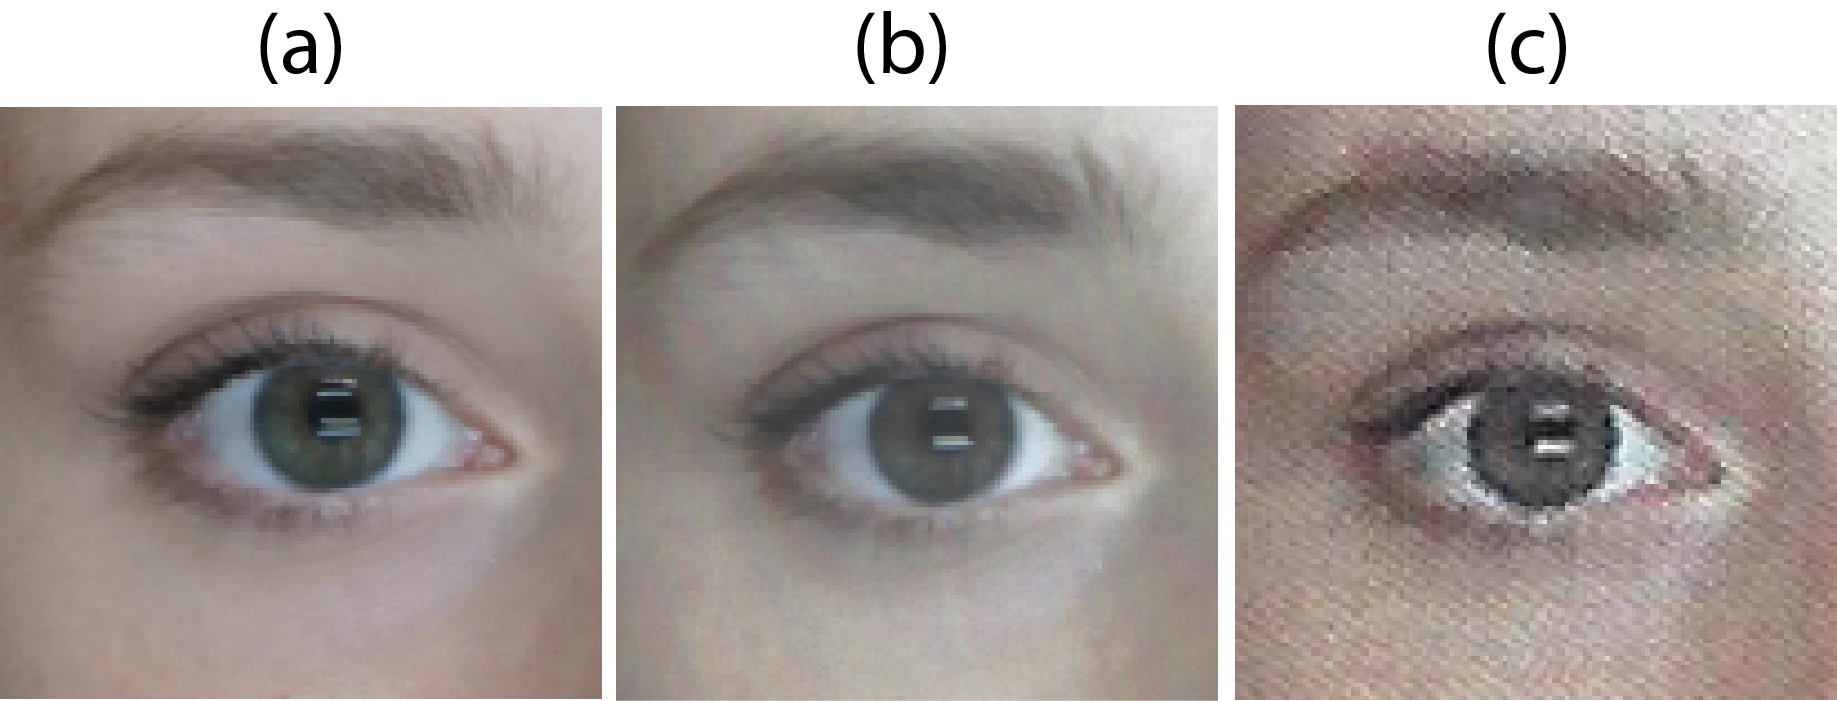
\includegraphics[width=0.8\textwidth]{ch-sistemasABC/images/ch-morphing/CalidadImpresas.png}
     \caption{(a) Calidad delas imágenes \Gls{FRAV-Morphing-Test}. (b) Calidad de las imágenes \Gls{FRAV-Morphing-Test-PS-300}. (c) Calidad de imágenes \Gls{FRAV-Morphing-Test-PS-150}.}
     \label{fig:NOISE_PrintScan}
\end{figure}

El proceso habitual para la expedición de pasaportes consiste en escanear una fotografía, previamente impresa, del viajero. Esto hace que la imagen almacenada finalmente el \text{<<\gls{chip}>>} del \gls{eMRTD} tenga una degradación que influye a la hora de detectar ciertos ataques, especialmente el \gls{morphing} (ver Fig. \ref{fig:NOISE_PrintScan}). Para evaluar la eficacia de los \GLS{MAD} en circunstancias reales se han construido dos conjuntos de datos con imágenes impresas y escaneadas.

Se seleccionan los $12$ sujetos de \Gls{FRAV-Morphing-Test} que consiguen un mejor \textit{score} de verificación con \gls{FaceNet} \cite{schroff2015facenet}, entre sus imágenes \gls{vivo} y los \gls{chip} \gls{morphing}. Es decir, aquellos que mejor consiguen engañar a un sistema reconocimiento facial.

Las $12$ imágenes \textit{<<\gls{chip}>> \gls{bona-fide}} y las $144$ imágenes \gls{chip} \gls{morphing} de los usuarios seleccionados se han impreso a $300$ \gls{DPI} con una impresora \textit{LaserJet} a color y a continuación se han escaneado para construir un nuevo conjunto de datos (\Gls{FRAV-Morphing-Test-PS-300}). También se repite el proceso de impresión y escaneado, esta vez a $150$ \gls{DPI} para construir \Gls{FRAV-Morphing-Test-PS-150}. (Ver contenido de las bases de datos \Gls{FRAV-Morphing-Test-PS-300} y \Gls{FRAV-Morphing-Test-PS-150} en la Tabla. \ref{tab:BASES_DE_DATOS_ORPHING}).

%%%%%%%5 PAD MULTI %%%%%%%%%%%%%%
\chapter{PAD multi-ataque y multi-sensor}\label{ch:PAD_MULTIATAQUE}

Existen muchos estudios que presentan diferente métodos para hacer frente a ataques de presentación pero la mayoría de ellos consideran sólo un numero limitado de tipos de ataque y un único sensor de captura.

En este capítulo se hace un análisis de los distintos métodos presentados en la literatura pero considerando distintos tipos de ataque de forma aislada y en conjunto. Además se evalúan también en capturas realizadas con diferentes sensores. Los ataques y los sensores considerados son los incluidos en la base de datos \textit{\Gls{FRAV-Attack}} presentada en la Sección \ref{subsec:FRAV-ABC-ATTACK}.

El objetivo es implementar un mecanismo de PAD que ofrezca una solución global para sistemas \GLS{ABC}, capaz de hacer frente a todas las posibles amenazas de ataques directos al sistema de captura.


Primero evaluamos cada uno de los algoritmos propuestos en la literatura para distintos ataques con todos los ataques considerados en \textit{\gls{FRAV-Attack}},


Como el sistema debe hacer frente a los distintos ataques contemplados se plantea una solución milimétrica con fusión a nivel \textit{scores} (Como se ve en la gráfica se consigue un mejor resultado en la fusión de \GLS{PAD} para cada tipo de ataque que un \GLS{PAD} para detectar todos los ataques en conjunto).

Los algoritmos se pueden agrupar en dos conjuntos 

\color{blue}La primera versión de este \GLS{PAD} se ha entrenado con imágenes de una base de datos construida en un laboratorio \textit{\Gls{FRAV-Attack}} que incluye tanto imágenes \gls{bona-fide} como imágenes con presentaciones de ataques con los \GLSpl{PAI} más comunes en la literatura (para ver más información sobre esta base de datos ver Sección \ref{sec:BBDD-FRAV-Attack}).\color{black}

%%%%%%%5 PREPROCESADO %%%%%%%%%%%%%%
\section{Preprocesado}\label{sec:PAD_PRERPROCESADO}

\begin{figure}
\centering
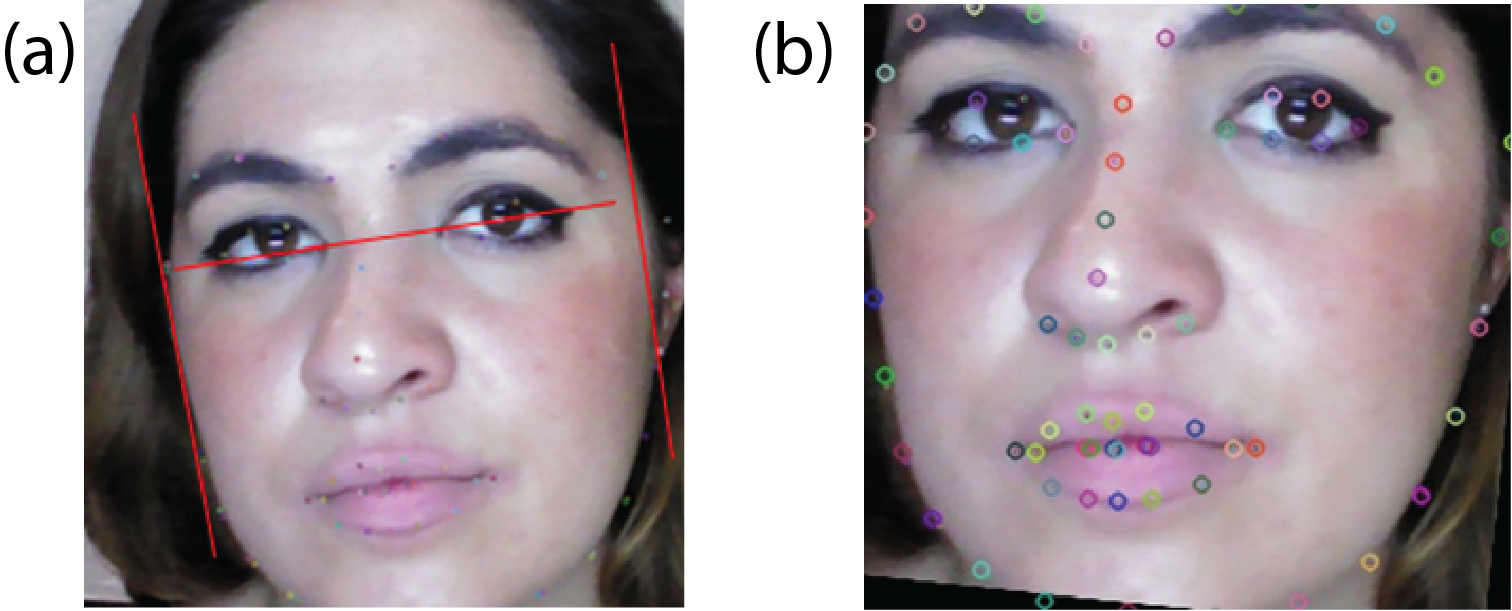
\includegraphics[width=1\textwidth]{ch-sistemasABC/images/ch-evaluacion_topologias/CORRECION_DE_POSE.png}
    \caption{Corrección de la pose de la cara.}
    \label{fig:CORRECCION_DE_LA_POSE}
\end{figure}

Se ajusta la cara atendiendo a la región delimitada por los \textit{landmarks} y se corrigen las posibles inclinaciones atendiendo a los \textit{landmark} de los ojos (Figura \ref{fig:CORRECCION_DE_LA_POSE}).

Con estos ajustes se ejecutan clasificaciones anteriores y se comparan los resultados para verificar si mejoran con el ajuste.

Para ello se ha seleccionado un tercio de la imágenes para entrenar la \GLS{SVM} y el resto para verificar los resultados. 

\textbf{Comparación de la clasificación con nube densa de profundidades} (Fig. X).

% \begin{figure}
% \centering
% 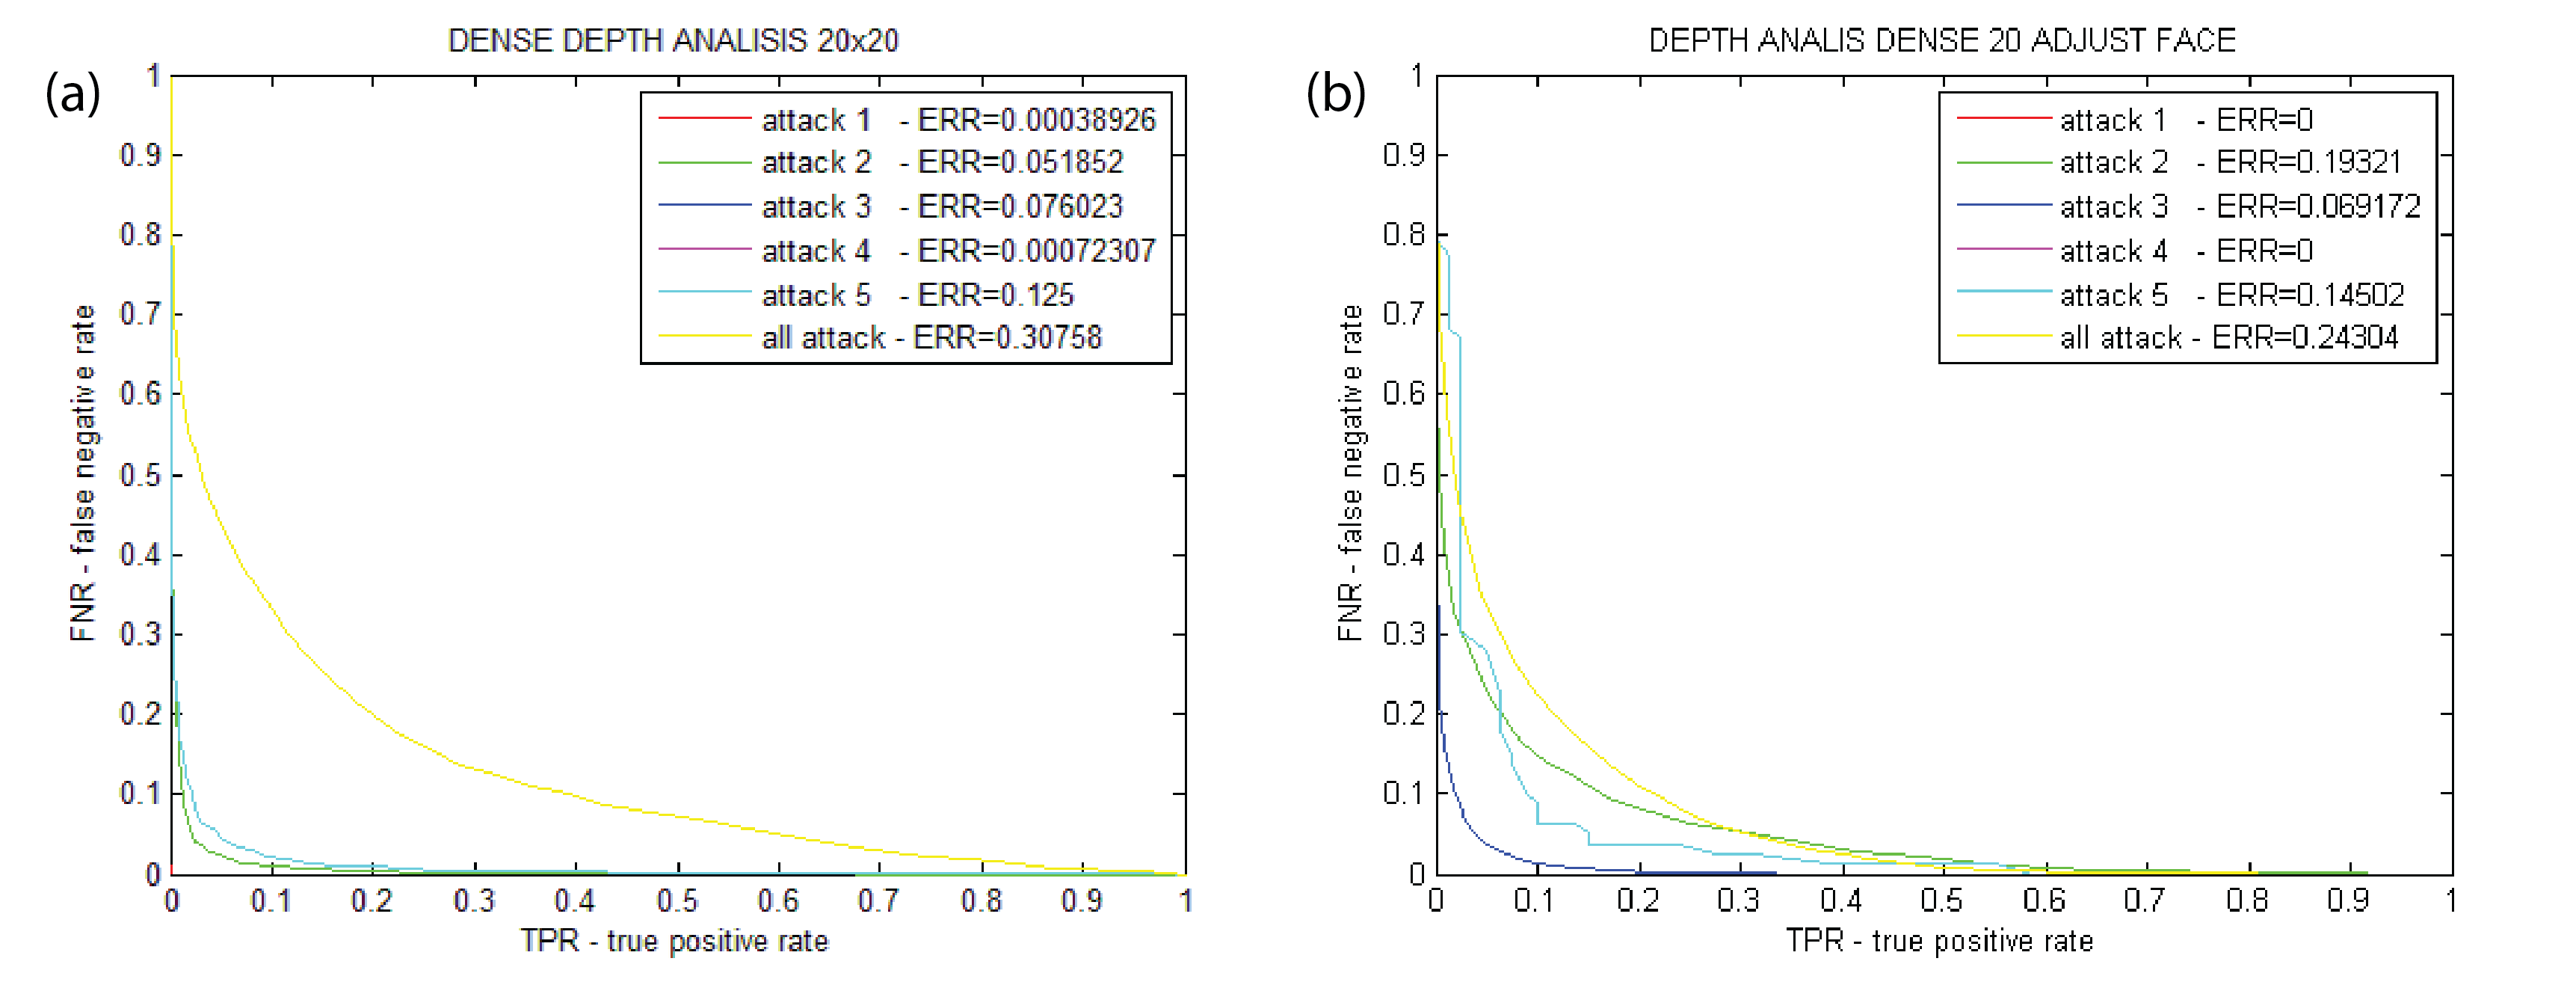
\includegraphics[width=1\textwidth]{ch-sistemasABC/images/ch-evaluacion_topologias/COMPARACION_DESA.png}
%     \caption{Comparación de los resultados considerando una nube densa de puntos, con corrección y sin corrección de la pose.}
%     \label{fig:COMPARACION_DENSA}
% \end{figure}

\textbf{Comparación de la clasificación con histogramas de profundidad por regiones}  (Fig, X). 
% \begin{figure}
% \centering
% 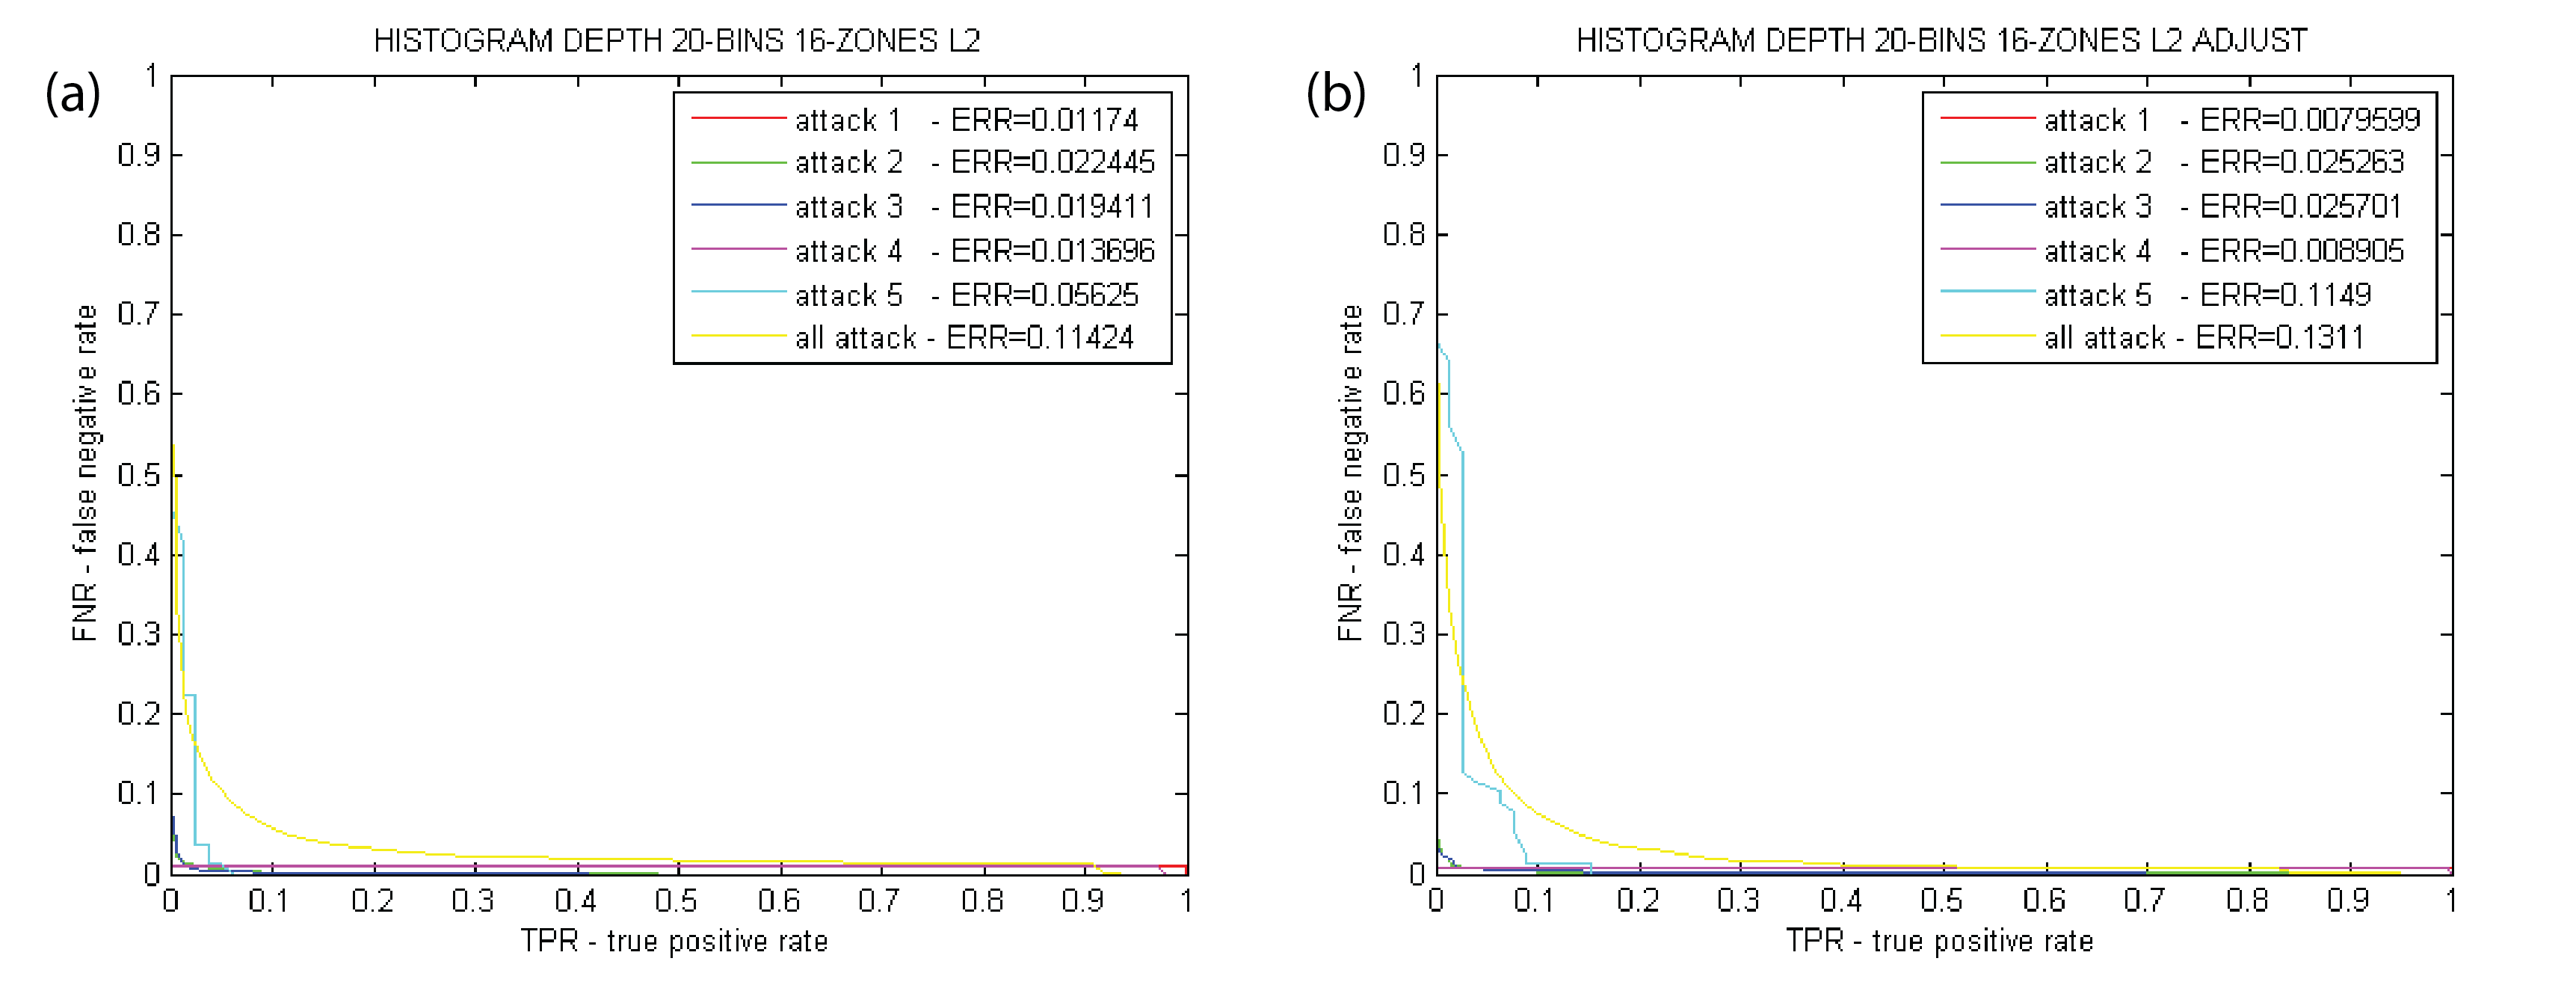
\includegraphics[width=1\textwidth]{ch-sistemasABC/images/ch-evaluacion_topologias/COMPARACION_HISTOGRAMA_REGIONES.png}
%     \caption{Comparación de los resultados considerando los histogramas por regiones, con corrección y sin corrección de la pose.}
%     \label{fig:COMPARACION_HISGRAMA_REGIONES}
% \end{figure}

%%%%%%%5 PAD BASADOS EN TEXTURAS %%%%%%%%%%%%%%
\section{Algoritmos basados en texturas}\label{sec:PAD_TEXTURAS}

\paragraph{\textbf{Clasificación basada en \textit{Depth} calculando \GLS{LBP}}}

Se calcula el \GLS{LBP} de las imágenes de profundidad. (Fig. x).

% \begin{figure}
% \centering
% 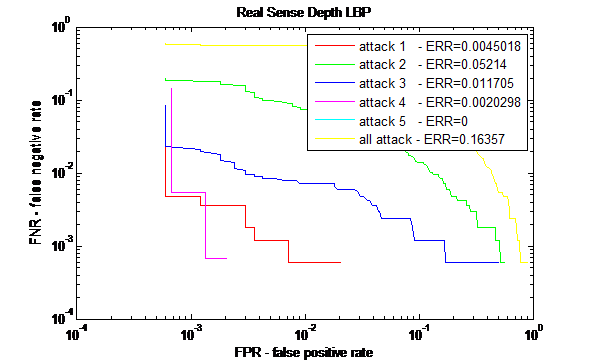
\includegraphics{ch-sistemasABC/images/ch-evaluacion_topologias/DET_LBP_PROFUNDIDAD.png}
%     \caption{\GLS{DET} del \GLS{SVM} de con \GLS{LBP} en la imagen de profundidad.}
%     \label{fig:DET_PROFUNDIDAD_LBP}
% \end{figure}

\paragraph{\textbf{Clasificación basada en \GLS{RGB} calculando \GLS{LBP}}}

% \begin{figure}
% \centering
%     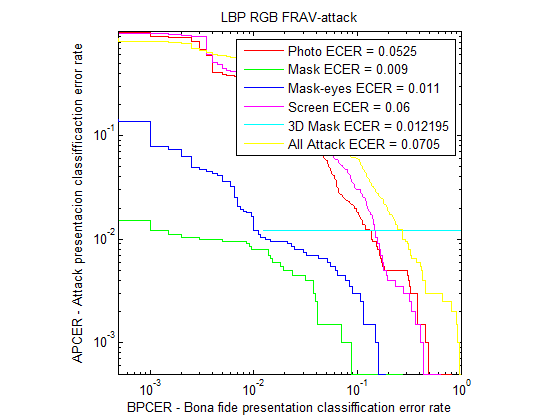
\includegraphics[width=1\textwidth]{ch-sistemasABC/images/ch-evaluacion_topologias/DET_LBP_RGB.png}
%     \caption{\GLS{DET} del \GLS{SVM} de con \GLS{LBP} en la imagen \GLS{RGB}.}
%     \label{fig:DET_RGB_LBP}
% \end{figure}

Se calcula el \GLS{LBP} de las imágenes \GLS{RGB} (Fig. X).

La nueva implementación consiste en localizar la cara con la imagen \GLS{RGB}, segmentarla, reducirla a $100\times100$ y calcular el histograma \GLS{LBP} con \GLS{OpenCV}.

Entrenar un \GLS{SVM} biclase con cada ataque frente a un usuario real. Y también una \GLS{SVM} con todos los ataques agrupados frente a un usuario real.

\color{black}

Los experimentos presentados este capitulo fueron realizados durante la implantación de los dispositivos pilotos del proyecto \GLS{ABC4EU} \cite{ABC4EUOnline}, del Séptimo Programa Marco de la \GLS{EU}. Los resultados obtenidos en dichos experimentos y las conclusiones extraídas se exponen en detalle en la sección \ref{sec:ResultadosABC4EU}. 

Experimentos en un entorno real (Aeropuerto Adolfo Suarez Madrid-Barajas \cite{aeropuertoMadridBarajas}) para evaluar y comparar el rendimiento de sistemas \GLS{ABC} con distintas topologías. 

El presente capitulo describe el piloto de un sistema de control automático de fronteras \GLS{ABC} desarrollado durante el proyecto \GLS{ABC4EU} y que se ajusta a las leyes establecidas para la zona \Gls{Schengen}.

Los dispositivos del sistema \GLS{ABC} analizados tienen una topología \textit{<<Segregated Two Step>>} (para mas información sobre este tipo de sistemas ver Sección \ref{subsec:Topologias}), con una configuración estructural dividida en dos dispositivos: el registro en un \gls{e-kiosk} y la verificación y el cruce de frontera en una \gls{e-gate} de tipo \gls{mantrap}. Esto implica dos etapas de captura y dos puntos sensibles en los que el sistema puede sufrir ataques de presentación. Las pruebas se llevaron a cabo con un piloto del sistema, en la terminal T$4$-S (satélite T$4$) del aeropuerto Adolfo Suárez de Madrid-Barajas, donde se capturó la base de datos \Gls{FRAV-ABC-Attack}.

Los experimentos ponen a prueba la seguridad del sistema simulando diferentes ataques de presentación, ambas etapas del sistema: registro y verificación. Loa ataques contemplados son los incluidos en \Gls{FRAV-ABC-Attack}: Foto, máscara, mascara sin ojos, vídeo, máscara $3$D y camiseta. (ver Sección \ref{subsec:FRAV-ABC-ATTACK}).

Finamente los resultados obtenidos para cada uno de los ataques se presenta en la Sección \ref{sec:ResultadosABC4EU}, indicando aquellos ataques que pueden resultar más peligrosos para el sistema y sugiriendo algunas contramedidas que podrían aumentar la fiabilidad y la seguridad del sistema.

%%%%%%%5 PAD BASADOS EN DESCRIPTORES %%%%%%%%%%%%%%
\section{Algoritmos basados en descriptores}\label{sec:PAD_DESCRIPTORES}

Analizamos la profundidad de imágenes recortadas con la región de la cara de cada fotograma.

Clasificación basada en el análisis de las profundidades de forma densa.

Se analiza una serie de puntos equidistantes distribuidos de forma densa por toda la imagen. De cada punto se toma la profundidad y se compone un vector con los valores de profundidad en cada punto. Estos vectores de características serán con los que entrenaremos la \GLS{SVM}.

Los pasos detallados del algoritmo son:
\begin{enumerate}
\item
Localización de la cara con \Gls{Viola-Jones} en la imagen \GLS{RGB}.

\item
Segmentación de la región de la cara en la matriz de profundidad que está registrada con la imagen \GLS{RGB}.

\item
Normalizamos los valores de profundidad para la región de la cara. Para ello:

Se seleccionan todas las profundidades distintas de $0$. (Las distancias $0$ son aquellas que no han podido ser calculadas por la cámara).

Se calcula la media y la desviación para establecer un límite máximo y mínimo de las profundidades a considerar.

% cv::meanStdDev(cleanDepth, mean, stddev);
% double cleanMin = mean.val[0] - 4 * stddev.val[0];
% double cleanMax = mean.val[0] + 4 * stddev.val[0]; 

Los puntos \textit{outlayers}, es decir los que tiene profundidades fuera de estos límites se establecen a $0$ y el resto de las profundidades se normalizan atendiendo a la profundidad máxima y mínima calculada.

% depthImage.at<float>(row, col) = (1 - ((depthImage.at<float>(row, col) - cleanMin) / (cleanMax - cleanMin))) * 255;

\item
Se reduce la matriz con las profundidades de la cara a un tamaño de $300\times300$.

\item
Se construye un vector con las profundidades de una serie de puntos distribuidos en una rejilla uniforme (por ejemplo, de $10\times10$) sobre la imagen. 

\end{enumerate}

\paragraph{\textbf{Clasificación basada en el análisis de las profundidades de forma densa}}

Imágenes de clasificación basada en el análisis de profundidad de las imágenes analizándola en el punto de interés (Figura \ref{fig:PUNTOS_DE_INTERES_EN_IMAGENES_DE_PROFUNDIDAD} y figura \ref{fig:PUNTOS_DE_INTERES_EN_IMAGENES_DE_PROFUNDIDAD_EN_ATAQUES}).

\begin{figure}
\centering
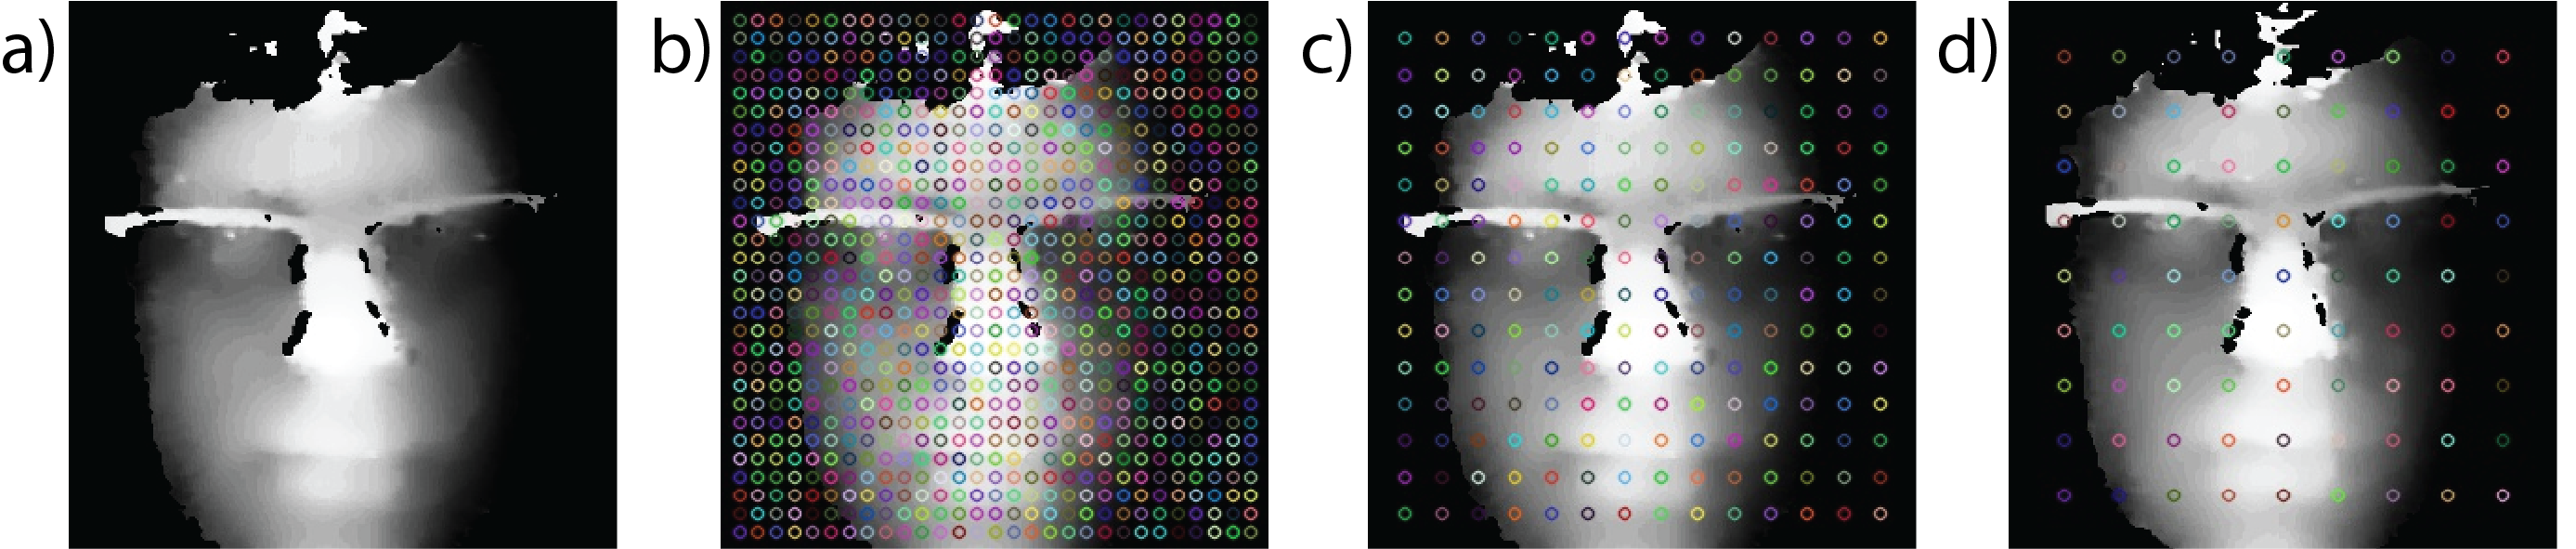
\includegraphics[width=1\textwidth]{ch-sistemasABC/images/ch-evaluacion_topologias/PUNTOS_DE_INTERES_EN_IMGS_PROFUNDIDAD.png}
    \caption{Puntos de interés en imágenes de profundidad.}
    \label{fig:PUNTOS_DE_INTERES_EN_IMAGENES_DE_PROFUNDIDAD}
\end{figure}
 
\begin{figure}
\centering
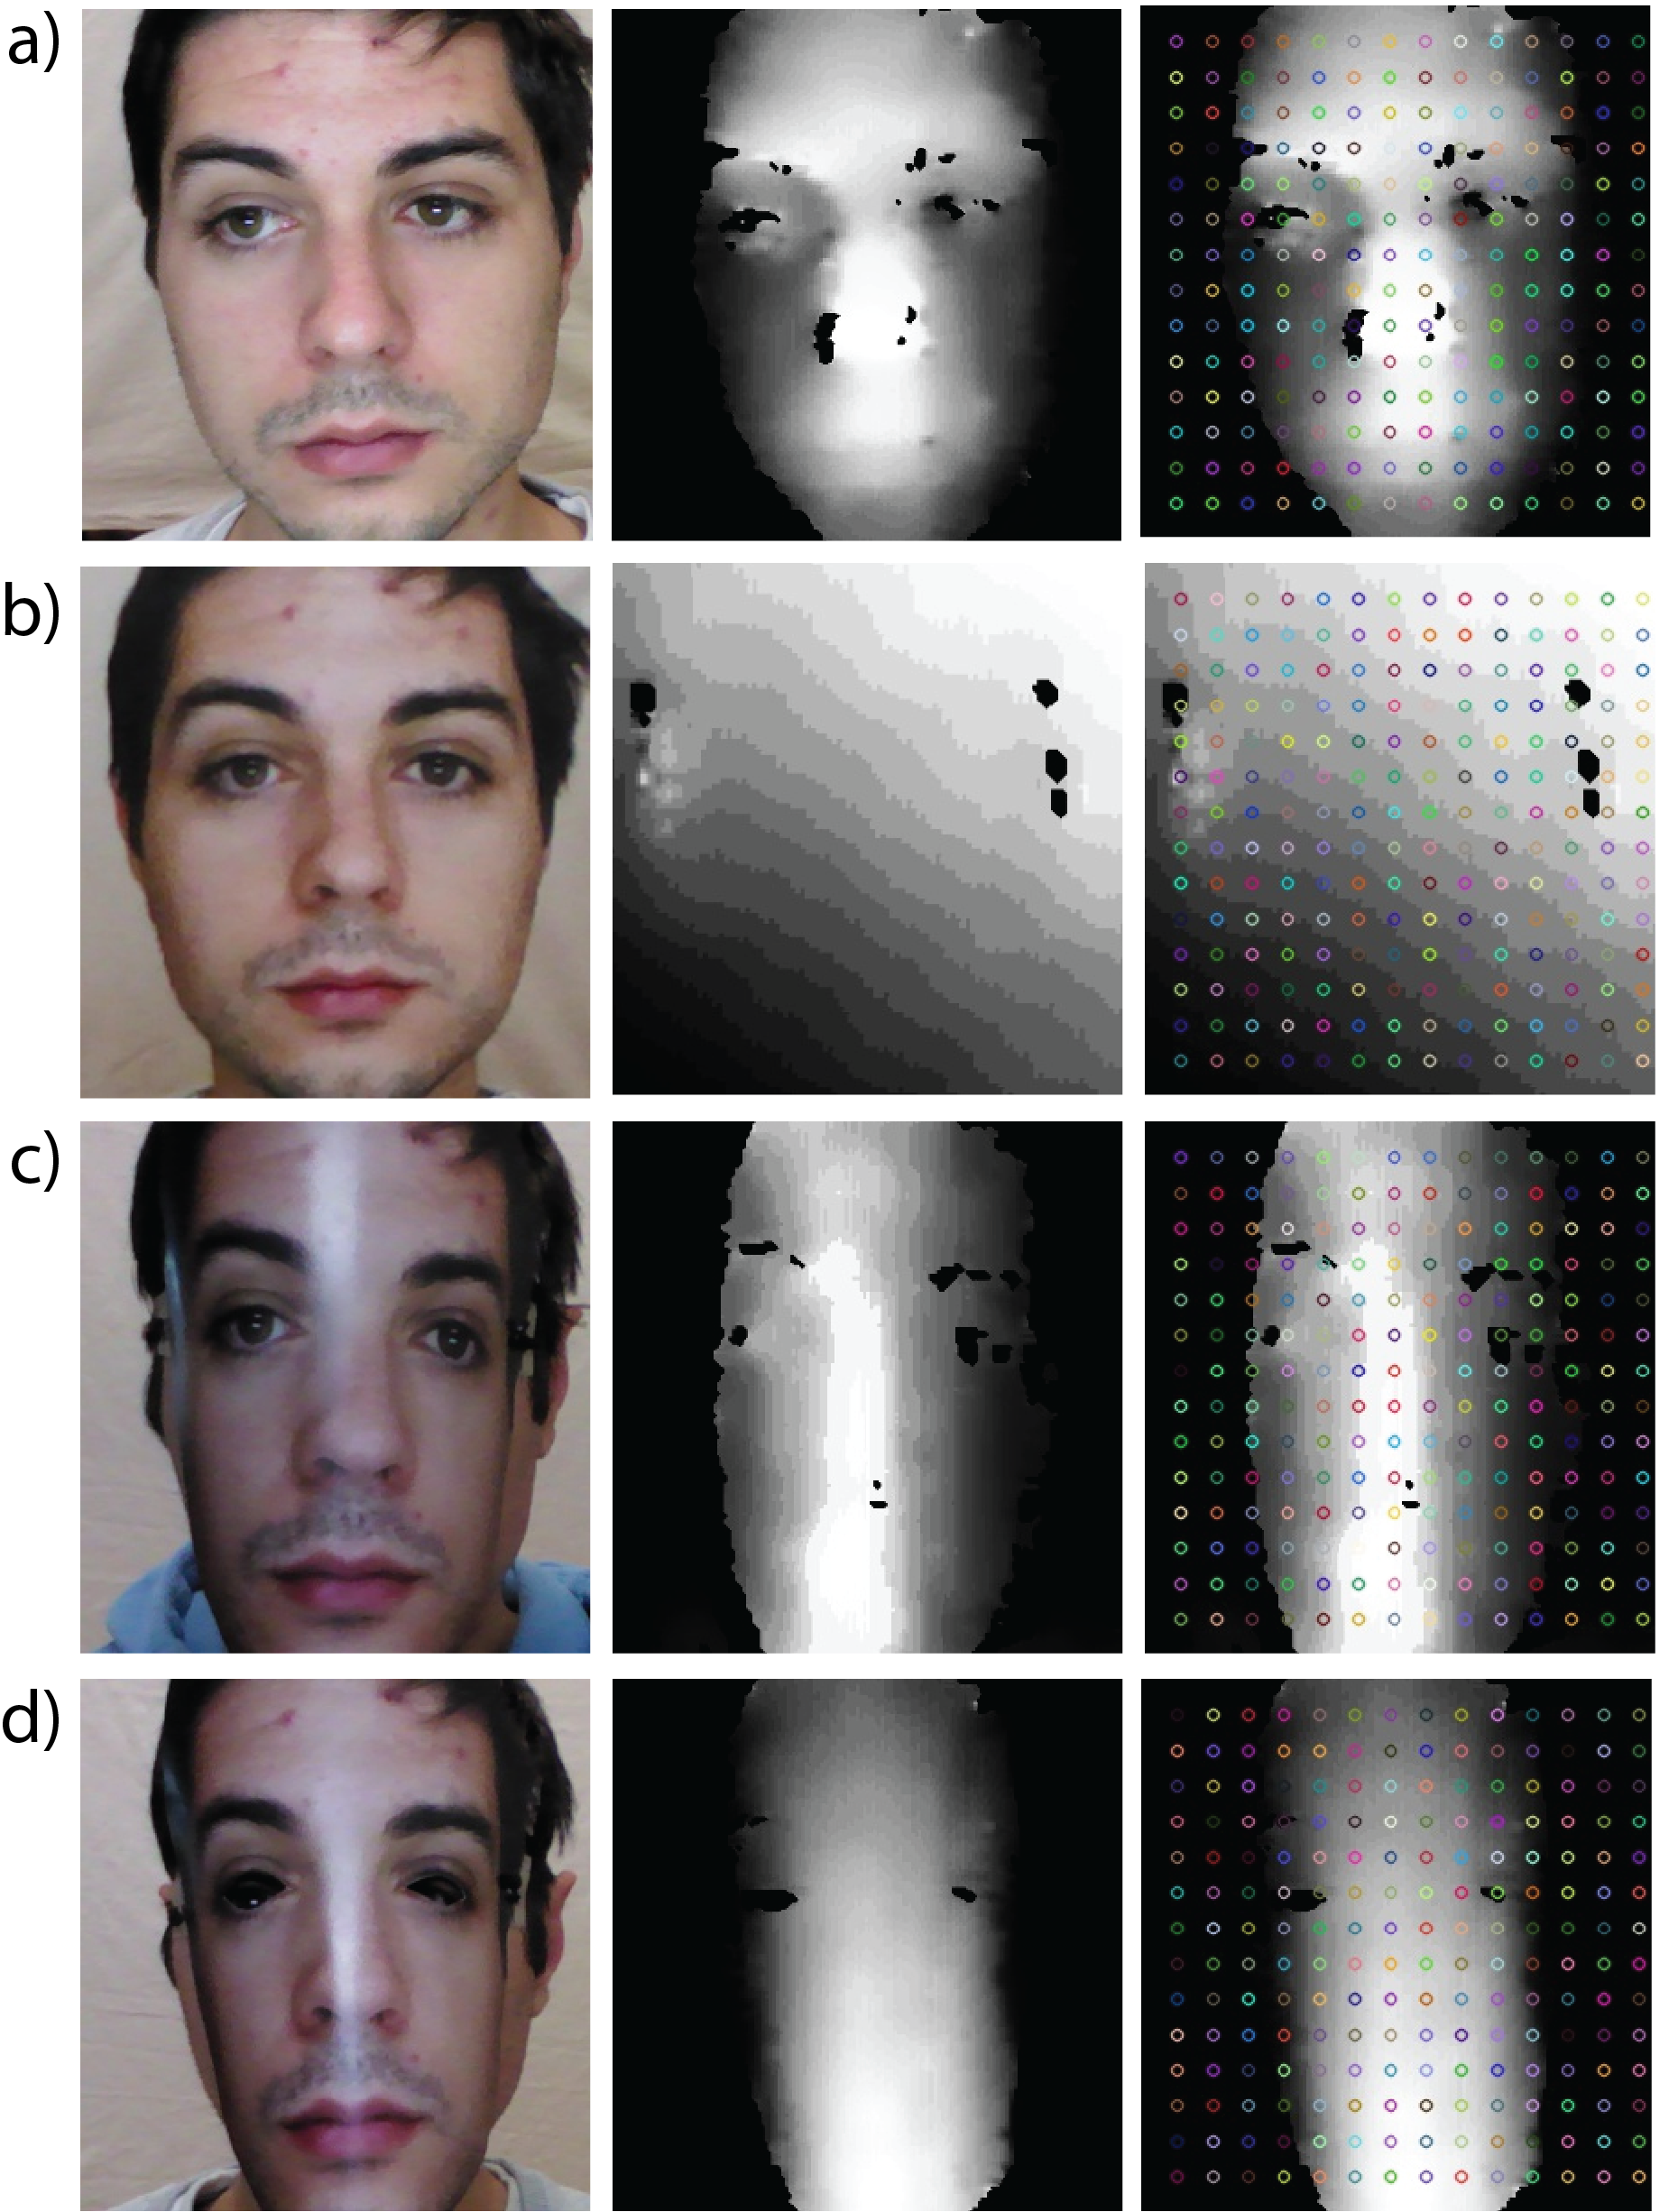
\includegraphics[width=0.6\textwidth]{ch-sistemasABC/images/ch-evaluacion_topologias/PUNTOS_DE_INTERES_EN_IMGS_PROFUNDIDAD_2.png}
    \caption{Puntos de interés en imágenes de profundidad en los distintos ataques de \Gls{FRAV-Attack}.}
    \label{fig:PUNTOS_DE_INTERES_EN_IMAGENES_DE_PROFUNDIDAD_EN_ATAQUES}
\end{figure}

Resultados de clasificación basada en el análisis de profundidad de las imágenes analizándolas con una nube de puntos densa (Figura \ref{fig:RESULTADOS_PROFUNDIDAD_DENSA}).

\begin{figure}
\centering
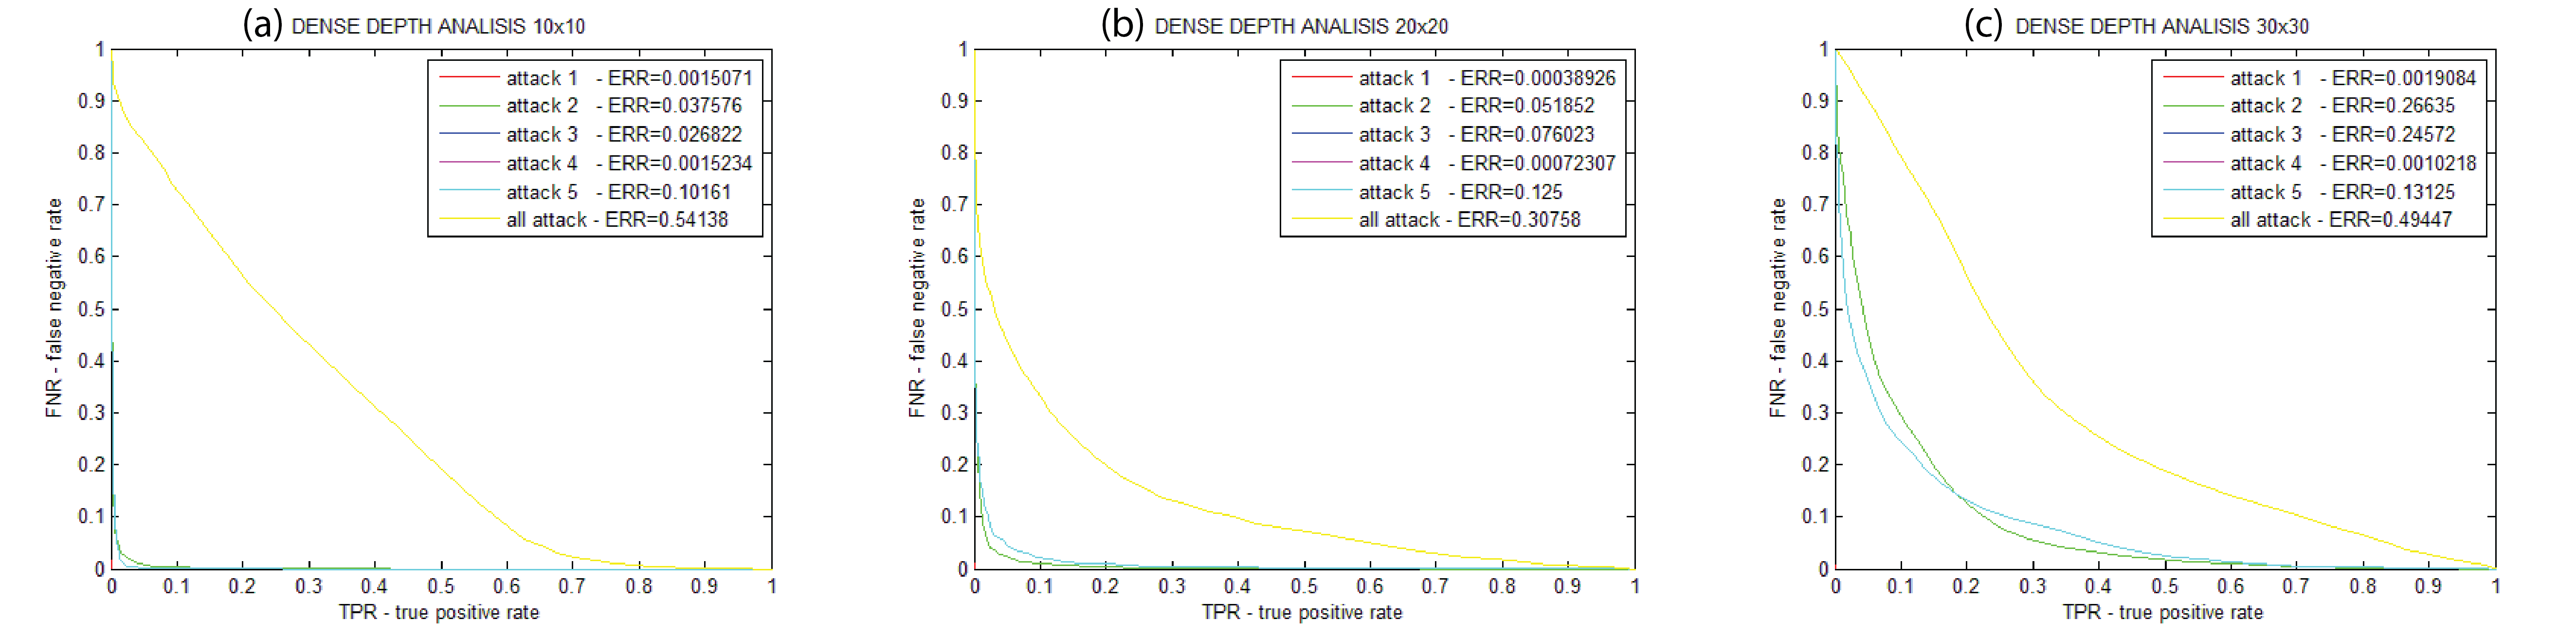
\includegraphics[width=1\textwidth]{ch-sistemasABC/images/ch-evaluacion_topologias/RESULTADOS_PROFUNDIDAD_DENSA.png}
    \caption{Resultados de clasificación basada en el análisis de profundidad de las imágenes analizándolas con una nube de puntos densa.}
    \label{fig:RESULTADOS_PROFUNDIDAD_DENSA}
\end{figure}

\paragraph{\textbf{Clasificación basada en el análisis de las profundidades en puntos de interés}}

Imágenes de clasificación basada en el análisis de profundidad de las imágenes analizándola en el punto de interés (Figura \ref{fig:SIFT_EN_IMAGENES_DE_PROFUNDIDAD_EN_ATAQUES}).

\begin{figure}
\centering
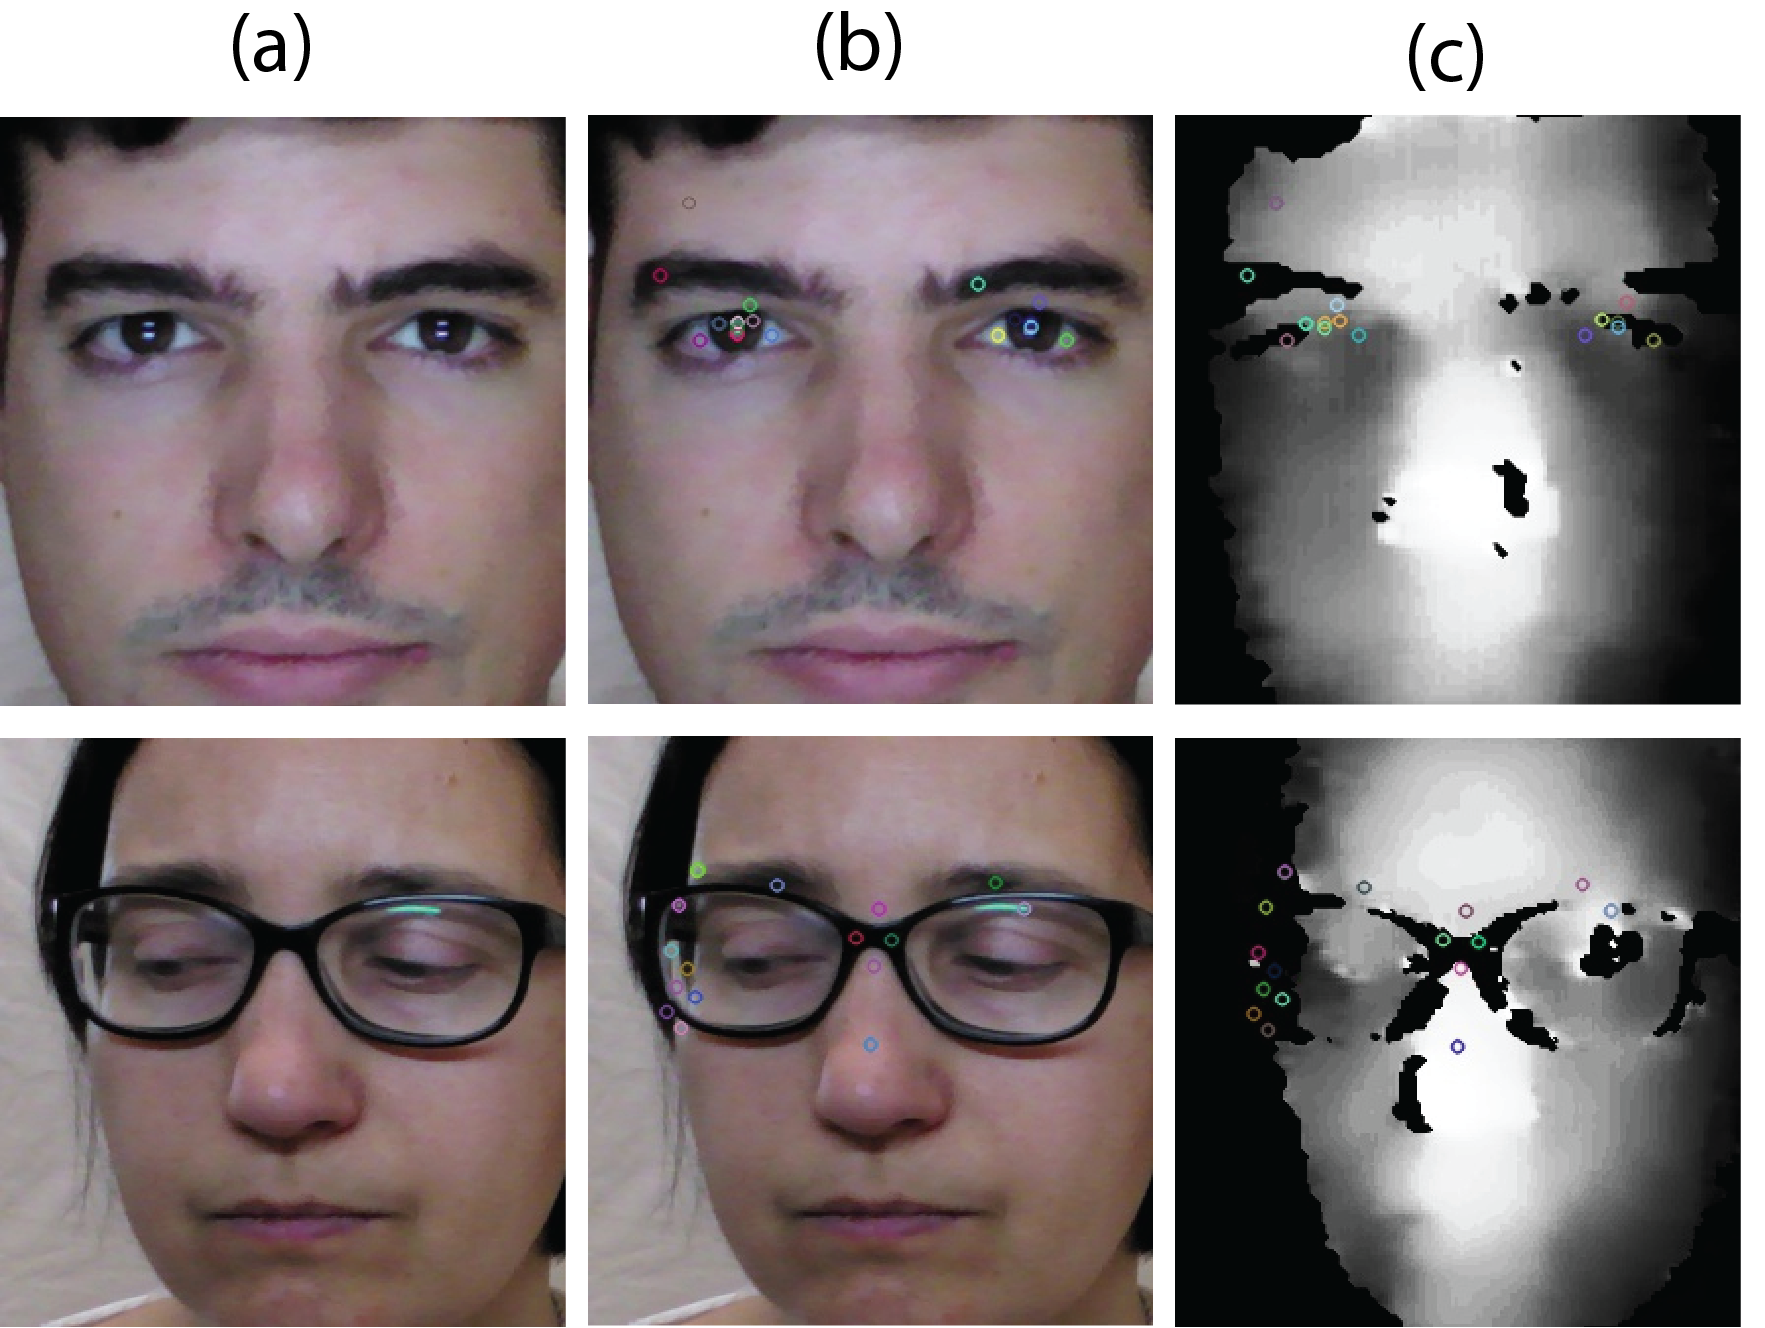
\includegraphics[width=0.6\textwidth]{ch-sistemasABC/images/ch-evaluacion_topologias/SIFT_EN_IMGS_PROFUNDIDAD.png}
    \caption{\gls{SIFT} en imágenes de profundidad en los distintos ataques de \textit{\Gls{FRAV-Attack}}.}
    \label{fig:SIFT_EN_IMAGENES_DE_PROFUNDIDAD_EN_ATAQUES}
\end{figure}

Resultados de clasificación basada en el análisis de profundidad de las imágenes analizándola en el punto de interés (Figura \ref{fig:RESULTADOS_PROFUNDIDAD_SIFT}).

\begin{figure}
\centering
\includegraphics[width=1\textwidth]{ch-sistemasABC/images/ch-evaluacion_topologias/RESULTADOS_PROFUNDIDAD_SIFT.png}
    \caption{Resultados de clasificación basada en el análisis de profundidad de las imágenes analizándola en el punto de interés.}
    \label{fig:RESULTADOS_PROFUNDIDAD_SIFT}
\end{figure}

\paragraph{\textbf{Clasificación basada en los histogramas de profundidad}}

Histogramas obtenidos de las imágenes de profundidad (Figura \ref{fig:HISTOGRAMAS_DE_PROFUNDIDAD}).

\begin{figure}
\centering
\includegraphics[width=1\textwidth]{ch-sistemasABC/images/ch-evaluacion_topologias/HISTOGRAMAS_DE_PROFUNDIDAD.png}
    \caption{Histogramas de profundidad.}
    \label{fig:HISTOGRAMAS_DE_PROFUNDIDAD}
\end{figure}

Resultados de clasificación basada en el análisis de profundidad de las imágenes analizándola en el punto de interés (Figura \ref{fig:RESULTADOS_HISTOGRAMAS_DE_PROFUNDIDAD}).

\begin{figure}
\centering
\includegraphics[width=1\textwidth]{ch-sistemasABC/images/ch-evaluacion_topologias/RESULTADOS_CLASIFICACION_POR_HISTROGRAMAS.png}
    \caption{Resultados obtenidos con los histogramas de profundidad.}
    \label{fig:RESULTADOS_HISTOGRAMAS_DE_PROFUNDIDAD}
\end{figure}

\paragraph{\textbf{Clasificación basada en los histogramas de profundidad teniendo en cuenta la información regional ($4$ regiones, $16$ regiones).}}

Se calcula el histograma con $20$ niveles de profundidad de cada una de estas regiones y se concatenan los histogramas.

Considerando $4$ particiones en la imagen y considerando la concatenación de los histogramas de $16$ regiones (Figura \ref{fig:HISTOGRAMAS_POR_REGIONES}).

\begin{figure}
\centering
\includegraphics[width=1\textwidth]{ch-sistemasABC/images/ch-evaluacion_topologias/HISTOGRAMAS_ANALIZADOS_POR_REGIONES.png}
    \caption{Considerando histogramas por regiones para conservar la información local.}
    \label{fig:HISTOGRAMAS_POR_REGIONES}
\end{figure}

Resultados de la clasificación basada en histogramas por regiones (Fig. \ref{fig:RESULTADOS_HISTOGRAMAS_POR_REGIONES} ).

\begin{figure}
\centering
\includegraphics[width=1\textwidth]{ch-sistemasABC/images/ch-evaluacion_topologias/RESULTADOS_HISTOGRAMAS_POR_REGIONES.png}
    \caption{Resultados obtenidos al considerar histogramas por regiones para conservar la información local.}
    \label{fig:RESULTADOS_HISTOGRAMAS_POR_REGIONES}
\end{figure}

\paragraph{\textbf{Clasificación basada en la profundidad de los puntos \textit{landmark} de la cara}}.

Se calculan los \textit{landmark} de la cara con la librería \Gls{Dlib}.

Se crea un vector con las profundidades de los puntos (ver Fig- \ref{fig:LANDMARK_DETECTADOS}). 

\begin{figure}
\centering
\includegraphics[width=1\textwidth]{ch-sistemasABC/images/ch-evaluacion_topologias/LANDMARK_DETECTADOS.png}
    \caption{\textit{landmark} faciales detectados.}
    \label{fig:LANDMARK_DETECTADOS}
\end{figure}

Se normaliza el vector de puntos (Se eliminan los \textit{outlayers} y se selecciona el máximo y el mínimo del vector CREO QUE ESTO NO ES CORRECTO DEBERÍA COGERSE LA MEDIA)

Los resultados obtenidos al considerar los \textit{landmark} son Fig. X. 

% \begin{figure}
% \centering
% \includegraphics[width=1\textwidth]{ch-sistemasABC/images/ch-evaluacion_topologias/RESULTADOS_OPTENIDOS_CON_LANDMARK.png}
%     \caption{Resultados obtenidos considerando los \textit{landmark} de la cara.}
%     \label{fig:RESULTADOS_CON_LANDMARK}
% \end{figure}


\chapter{Sistemas PAD para ABC \textit{<<Segregated Two Step>>}}\label{ch:EVALUACIONACION_TOPOLOGIAS}

A lo largo de este capítulo se describe el método \GLS{PAD} para sistemas \GLS{ABC} \textit{<<Segregated Two Step>>}, presentado en \textit{$14$th International Conference on Security and Cryptography, SECRYPT 2017}  \cite{del2017face}. La solución propuesta se diseñó e implantó en los sistemas pilotos \GLS{ABC} del proyecto a \GLS{ABC4EU}. En la Sección \ref{sec:SisABC4EU} se describe la operativa de este tipo sistemas que al tratarse de sistemas \textit{<<Segregated Two Step>>} requieren de dos verificaciones biométricas, es decir dos puntos débiles para ataques de presentación (para ver mas información sobre este tipo de sistemas ver Sección \ref{subsec:Topologias}). En el la Sección \ref{sec:PADSegregado} se describe el método \GLS{PAD} propuesto. En el apartado \ref{sec:ExperimentosABC4EU} se describen los experimentos realizados y a continuación los resultados obtenidos se detallan en la Sección \ref{sec:ResultadosABC4EU}. 


%%%%%  ABC de ABC4EU %%%%%%%%
\section{Sistemas ABC4EU}\label{sec:SisABC4EU}

\begin{figure}
\centering
    \includegraphics[width=\textwidth]{ch-sistemasABC/images/ch-evaluacion_topologias/ARQUIETECTURA_ABC_ABC4UE.png}
    \caption{Esquema de \GLS{ABC4EU}.}
    \label{fig:EsquemaABC4EU}
\end{figure}

Los sistemas \GLS{ABC4EU} son sistemas \GLS{ABC} \textit{<<Segregated Two Step>>}, con una etapa de registro \GLS{RTP} que puede realizarse de forma remota, para las pruebas se realizo de forma presencial en un \gls{e-kiosk} y una etapa de validación \GLS{EES} que se realiza en un \gls{e-gate} al cruzar la frontera (ver Fig. \ref{fig:EsquemaABC4EU}). 

\subsection{Registro: \textit{e-kiosk}}

\color{blue}Los \GLS{ABC} analizados son el prototipo de sistema propuesto en el proyecto \GLS{ABC4EU} por lo que ha sido posible evaluar el sistema en varios cruces de frontera reales durante la implantación de los pilotos del proyecto.
El proyecto europeo \GLS{ABC4EU} propone sistemas \GLS{ABC} para las fronteras de la \GLS{EU}. Los sistemas que propone es del tipo \GLS{ABC} \textit{<<Segregated Two Step>>}.\color{black}

En el registro el viajero presenta su \Gls{eMRTD}, el sistema lee sus datos del \gls{chip}. El proceso contrasta los datos del viajero con las bases de datos correspondientes, y certifica que el viajero es el verdadero titular del documento. Para ello, el sistema valida los datos biométricos \gls{chip} almacenados en el documento con los datos biométricos capturados en ese momento del registro (\gls{vivo registro}).

Cuando el proceso de registro ha realizado todos las comprobaciones con éxito, el sistema almacena los datos del viajero registrado durante un período limitado de tiempo, dependiendo del tipo de viajero. Durante este periodo, el viajero puede acceder a la \gls{e-gate} y cruzar la frontera si supera la etapa de validación.

\color{blue}Este sistema tiene operativas distintas dependiendo del tipo de viajeros: Si necesitan un visado o son viajeros frecuentes.

La operativa se compone de dos etapas el \GLS{RTP} y \GLS{EES} que llamaremos registro y validación.

Cada una de estas etapas tiene una verificación facial: en registro la verificación se realiza en entre la imagen de \gls{chip} y una imagen capturada en es momento \gls{vivo registro} y en validación la verificación se realiza entre la imagen \gls{vivo registro} y una nueva imagen que se captura del viajero en la \gls{e-gate} \gls{vivo validacion}. (ver Fig. \ref{fig:EsquemaABC4EU})


Los sistemas\GLS{ABC} \textit{<<Segregated Two Step>>} realizan los procesos \GLS{RTP} y \GLS{EES} en dos dispositivos distintos un \gls{e-kiosk} y una \gls{e-gate} (para más información sobre estos procesos ver Sección \ref{subsec:ArquitecturaLogicaABC}). Cada uno de estos dispositivos tiene un sistema de captura en el que se realiza una verificación facial.

En la etapa de \GLS{RTP} una verificación facial entre el \gls{chip} del pasaporte y una imagen de viajero capturada en el registro (\gls{vivo registro}) y en la etapa \GLS{EES} una verificación entre el \gls{vivo registro} capturado en la etapa anterior y una nueva imagen capturada en ese momento en la \gls{e-gate} (\gls{vivo validacion}).
\color{black}

El sistema considera dos protocolos diferentes dependiendo del tipo de viajero. Por un lado, los viajeros \GLS{TCNVE} que pueden hacer el registro  en el \gls{e-kiosk} al llegar al aeropuerto antes de su viaje. Y por otro lado, los viajeros \GLS{TCNVH}, que no pueden hacer el registro en el aeropuerto y obligatoriamente deben registrarse en el sistema en su consulado antes de la etapa de verificación en el aeropuerto. También, los viajeros \GLS{TCNVE} que sean viajeros frecuentes, pueden registrarse en el sistema, en su consulado y se evitan realizar un registro en cada viaje. 

\subsection{Validación: \textit{e-gate}}

El proceso de validación siempre tiene lugar en la \gls{e-gate} después de la etapa de registro. La etapa de validación consiste en comparar una nueva captura de los datos biométricos del viajero \gls{vivo validacion} con los datos biométricos capturados en la etapa del registro \gls{vivo registro}.

Tanto el los viajeros \GLS{TCNVE} como los viajeros \GLS{TCNVH} deben pasar esta etapa.

%%%%%  PAD SEGREGADO %%%%%%%%
\section{PAD \textit{<<Segregated Two Step>>}}\label{sec:PADSegregado}

\begin{figure}
    \centering
    \includegraphics[width=\textwidth]{ch-sistemasABC/images/ch-evaluacion_topologias/ESCENARIOS_VERIFICACION_DOS_PASOS_VER.png}
    \caption{Escenarios de verificación en sistemas \GLS{ABC} \textit{<<Segregated Two Step>>}.}
    \label{fig:escenariosVerifacionABC}
\end{figure}

Los ataques de presentación se producen en la fase de captura a nivel del sensor del subsistema biométrico (Ver Sección \ref{sec:ContextoAtaquesPresentacion}). Como los sistemas \GLS{ABC} del proyecto \GLS{ABC4EU} están organizados en dos etapas segregadas, se realizan dos capturas diferentes: una en el \gls{e-kiosk}, para el registro y la otra en la \gls{e-gate}, para la validación. Esto hace que el sistema tenga dos puntos vulnerables y que sea necesario considerar tres escenarios diferentes para un posible ataque (ver Fig. \ref{fig:escenariosVerifacionABC}).

\begin{itemize}
    \item
    \textit{Enrolment Presentation Attack} (\GLS{EPA}): Cuando el ataque se produce en la etapa de registro. Por ejemplo, un atacante se registra en el sistema con una documentación que pertenece a otra persona tratando de hacerse pasar por el verdadero titular de los documentos.
    \item
    \textit{Verification Presentation Attack} (\GLS{VPA}), Cuando el ataque de presentación se produce en la etapa de verificación. Un el atacante intenta hacerse pasar por un viajero que se ha registrado previamente en el sistema. Por ejemplo, cuando un viajero registrado correctamente pierde o le roban sus documentos entre la etapa del registro y la etapa de verificación. Entonces un atacante usa esos documentos para intentar para pasar la verificación.
    \item
    \textit{Enrolment and Verification Presentation Attack} (\GLS{EPA}+\GLS{VPA}). En este caso se trata de un doble ataque, la suplantación tiene lugar en el momento del registro y en la etapa de verificación, el atacante continúa haciéndose pasar por el verdadero viajero. Por ejemplo, un atacante presenta la documentación de otra persona y se registra con éxito. Y posteriormente, en la etapa de verificación, continúa haciéndose pasar por el verdadero poseedor de la documentos para cruzar la frontera.
\end{itemize}

Estos tres escenarios complican la evaluación del subsistema \GLS{PAD}.

En Fig. X a se pueden ver las curvas \GLS{ROC} de los resultados obtenidos en la verificación facial del registro, con distintos reconocedores faciales \GLSpl{COT}. Y en Fig. X b las curvas con los resultados obtenidos en la verificación  de la validación, con los mismos \GLSpl{COT}. En ambos caso los resultados son muy buenos, algo mejores en validación ya que el en esta etapa la verificación se realiza se realiza entre dos capturas relativamente recientes, \gls{vivo registro} y \gls{vivo validacion}. mientras que en registro la imagen \gls{chip} del pasaporte puede ser muy antigua (los pasaportes tienen distintos periodos de validez).
\color{red}figura con los \textit{score} de dgp de dos empresas que realmente son ABCS\color{black}

Cada uno de las gráficas de la figura Y muestra tres distribuciones de densidad de \textit{scores} obtenidos con uno de los reconocedores \GLSpl{COT} usados en las verificaciones del sistema: la distribución con los \textit{scores} de cruces negativos (en rojo), \textit{scores} de cruces positivos (en verde) y \textit{scores} de cruces de ataque (en azul). En cada una de las gráficas los \textit{scores} de ataque corresponde a cruces con tipo de \GLS{PAI} diferente. Como se puede ver en todas ellas el umbral que serviría para distinguir cruces positivos de cruces negativos (se ha elegido el umbral del \GLS{EER}) hace que los ataques sean considerado como cruces positivos lo que indica que los reconocedores empleados pueden ser engañados fácilmente con casi cualquier tipo de ataque.
\color{red}figura con una matriz de distribuciones, una por ataque los \textit{scores} de dgp de dos empresas que realmente son ABCS\color{black}

Cuando se pone a prueba el sistema con ataques se observa la cantidad de ataques que se cuelan ver tabla \color{red}quizás una tabla con los ataque que se cuelan\color{black} y por eso es imprescindible un sistema de detección de ataques de presentación. En la tabla se puede ver que ataques resultan más peligrosos. Además se puede apreciar que la validación es más sensible a los ataques que el registro. Esto se explica por las imágenes que se usan para realizar cada una de las verificaciones. A la hora de realizar los \GLS{PAI} se suelen usar imágenes mas recientes por lo que \gls{vivo validacion ataque} sera más parecido a \gls{vivo registro} que el propio \gls{vivo registro} a la imagen \gls{chip} del pasaporte.

Se propone un sistema \GLS{PAD} como el descrito en el capitulo \ref{ch:PAD_MULTIATAQUE} tanto para la etapa de registro como para la validación. Primero se entreno con la base de datos de \Gls{FRAV-Attack} (ver \ref{sec:BBDD-FRAV-Attack})  que incluye distintos tipos de ataques y se puso a prueba en los sistemas \GLS{ABC4EU} en un cruce de frontera real (Se pueden ver los datos obtenidos en la etapa de registro y en la etapa de validación).
Posteriormente se volvió a entrenar, esta vez con los datos capturados en el escenario real con los que se construyó un subconjunto de \Gls{FRAV-ABC-Attack} con imágenes \gls{vivo registro} e imágenes \gls{vivo validacion} (ver \ref{subsec:FRAV-ABC-ATTACK-DOS_PASOS}). Como era de esperar Los resultados del sistema entrenado con imágenes capturadas en el propio sistema mejoran mucho.


%% EXPERIMENTOS %%%%
\section{Experimentos realizados}\label{sec:ExperimentosABC4EU}

Los sistemas \GLS{ABC4EU} capturan la huella dactilar y una imagen de la cara en el sistema biométrico subsistema. Algunos estudios se han centrado en la verificación dactilar con este tipo de sistemas  \cite{donida2016emerging}, pero este estudio se centra en el reconocimiento facial por dos razones. Por un lado, la imagen de la cara es la única biométrica referencia obligatoria en todos pasaportes en el mundo (en la zona \Gls{Schengen} también el huellas dactilares de la mano izquierda). Y por otro lado, la cara es un rasgo que, en caso de error un agente siempre puede contrastar la información con una fácil inspección visual. Los experimentos realizados analizan los ataques en el registro (\GLS{EPA}) y en la validación (\GLS{VPA}), ambos de forma aislada aislamiento.

Para el registro, se emplearon pasaportes originales y todos los \GLS{PAI} se construyeron con características biométricas de $9$ propietarios legítimos de esos pasaportes. Así, cada \gls{chip bona-fide} se verificó con un \gls{vivo bona-fide} y con $6$ \gls{vivo ataque} con diferentes \GLS{PAI}. 

En la validación, sólo los casos en los que el registro se ha hecho con un \gls{bona-fide} se utilizan presentaciones. De esta manera, una presentación \gls{bona-fide} La presentación (\gls{vivo registro}) se cruza contra una presentación de \gls{bona-fide} (muestra \gls{vivo validacion} y contra 6 ataques con diferentes \GLSpl{PAI}.

El \GLS{PAD} devuelve la probabilidad de que la presentación sea un \gls{bona-fide}.

Para verificar la integridad del sistema contra el y analizar los datos obtenidos por el \GLS{PAD}, se han calculado las curvas \GLS{DET} con el resultado  obtenido de \GLS{APCER} y \GLS{BPCER}. 

Por razones de seguridad (el piloto fue realizado en una zona crítica con una frontera real cruce), la cantidad de sujetos de prueba era limitada. Esta restricción es la razón por la que se ha reducido relativamente el número de número de algunos de los ataques Durante la etapa de registro, véase el cuadro $2$, $61$ se hicieron presentaciones con $6$ viajeros diferentes, teniendo en cuenta los intentos de presentaciones de buena fe y ataques con los diferentes \GLS{PAI}. En la validación, se hicieron $93$ presentaciones en total, pero vamos a sólo usan 48, aquellos en los que se hizo el registro con una presentación \gls{bona-fide}. Se han ignorado el escenario de doble ataque (\GLS{EPA}+\GLS{VPA}).

%%%%%%%%%%%% RESULTADOS %%%%%%%%%%%%%%%%%%%%%%%%
\section{Resultados}\label{sec:ResultadosABC4EU}

\begin{table}
\centering
\begin{tabular}{|l|c|c|}
\hline
\GLS{PAI} & \GLS{D-EER} (registro) & \GLS{D-EER} (verificación) \\ \hline
\textbf{Foto} & $0.2000$ & $0.2071$ \\ \hline
\textbf{Máscara} & $0.0333$ & $0.2071$ \\ \hline
\textbf{Pantalla} & $0.1505$ & $0.1714$  \\ \hline
\textbf{Máscara $3$D} & $0.0000$ & $0.0000$  \\ \hline
\textbf{Morphing} & $0.0000$ & $0.5000$  \\ \hline
\textbf{Camiseta} & $0.2583$ & $0.0000$  \\ \hline
\textbf{Todos los \GLSpl{PAI}} & $0.1210$ & $0.2106$ \\ \hline
\end{tabular}
\caption{Error de detección \GLS{D-EER} obtenido con cada uno de los \GLS{PAI} en la etapa de registro y etapa de verificación.}
\label{tab:EPCERRegistroVerificacion}
\end{table}


\begin{figure}
\centering
    \includegraphics[width=1\textwidth]{ch-sistemasABC/images/ch-evaluacion_topologias/APCER_BPCER_CURVE_ENROLMENT.png}
    \caption{Curva \GLS{DET} con \GLS{APCER}-\GLS{BPCER} en la etapa de registro (Escenario \GLS{EPA}).}
    \label{fig:APCERBPCERRegistro}
\end{figure}

\begin{figure}
\centering
    \includegraphics[width=1\textwidth]{ch-sistemasABC/images/ch-evaluacion_topologias/APCER_BPCER_CURVE_IN_THE_VERIFICACION.png}
    \caption{Curva \GLS{DET} con \GLS{APCER}-\GLS{BPCER} en la etapa de registro (Escenario \GLS{VPA}).}
    \label{fig:APCERBPCERVerificacion}
\end{figure}

\color{blue}Se presentan los resultados de las dos verificaciones faciales que se realizan: Una la etapa de registro y otra en la etapa de cruce. También se analiza la resistencia a ataques de presentación en ambas etapas.\color{black}

En la Tabla \ref{tab:resultadosEnRegistro} se pueden ver los valores \GLS{APCER}, \GLS{BPCER} y el \GLS{D-EER} del \GLS{PAD} para diferentes umbrales en el registro y en la Tabla \ref{tab:resultadosEnVerificacion} los mimos umbrales en la validación. La disminución del \GLS{APCER} implica un aumento del \GLS{BPCER}, pero primando la seguridad como objetivo, un umbral de $80$ en el registro y $95$ en la validación sería el más adecuado. Como se puede ver en ambas tablas la tabla, esos dos umbrales son aproximadamente el \GLS{D-EER} en cada escenario.

En Fig. (\ref{fig:APCERBPCERRegistro}), se presenta la curva \GLS{DET} de \GLS{APCER}-\GLS{BPCER} para lo ataques en la etapa de registro. Se presentan los resultados considerado cada tipo de \GLS{PAI} de forma aislada y también con  todos los ataques en conjunto. La Fig. \ref{fig:APCERBPCERVerificacion} presenta la misma información para la etapa de validación en la \gls{e-gate}. En la curva obtenida para la etapa de registro (Fig. \ref{fig:APCERBPCERRegistro}), se observa que los ataques más peligrosos son los realizados con un dispositivo de vídeo y los ataques de fotografías (el ataque con camiseta tiene más \GLS{APCER} pero este resultado probablemente sea debido a la escasez de presentaciones disponibles con ese \GLS{PAI}), mientras que los otros ataques son fácilmente detectables en esta etapa. Aunque en verificación la mayoría de los ataques tienen un \GLS{APCER} más alto que en registro, el orden de  peligrosidad de los ataques se mantiene (ver Fig. \ref{fig:APCERBPCERVerificacion}). Este comportamiento (dejar pasar más ataques en verificación que en registro) puede explicarse la imagen de referencia que se usa para en cada etapa. , en el registro, el \gls{chip} del pasaporte, mientras que en la validación, la imagen de referencia es la \gls{vivo registro}. 

La baja calidad de las características biométrica presentada en el \gls{chip} del pasaporte dificulta la detección de ataques \gls{morphing} que en el caso de una imagen \gls{vivo} recientemente adquirida usada en la puerta electrónica. 

Con los resultados, es posible ver que para la mayoría de de los ataques, el \GLS{BPCER} en el registro es mayor que en validación. Esto indica que el registro es menos amigable y rechazará más presentaciones, incluso si cuando son  presentaciones \gls{bona-fide}.

En general, los valores \GLS{D-EER} de las pruebas realizadas en el registro son más bajos que en la validación (Tabla \ref{tab:EPCERRegistroVerificacion}). Esto indica que la etapa de registro es más robusta frente a ataques que la etapa de validación, es decir, se han clasificado menos ataques como \gls{bona-fide} (\GLS{APCER}) y también menos presentaciones \gls{bona-fide} como ataques (\GLS{BPCER}). Todo esto muestra que es mejor el uso de la información biométrica de los pasaportes como referencia para detectar ataque (muestra \gls{chip} vs. muestra \gls{vivo registro}), es más fiable que la comparación de la captura \gls{vivo validacion} con la captura \gls{vivo registro}, dos actuales imágenes del viajero.

La razón de esta diferencia es que los \GLS{PAI} para los ataques se construyen normalmente con fotos más recientes  del viajero. Por ejemplo, en los experimentos realizados, los \GLS{PAI} se construyeron con fotos tomadas pocos días antes. Esto significa que las diferencias entre el \GLS{PAI} y la apariencia del viajero actual se añade a la diferencia entre la imagen más antigua del pasaporte (en euro unos 7 años de vigencia de los pasaporte) y el aspecto actual del viajero.

%%%%%%%%%%%%%%%% CONCLUSIONES %%%%%%%%%%%%%%%%%%%%%%%%%
% \section{Conclusiones}\label{sec:ConclusionesABC4EU}

En este capítulo,se han presentado los resultados de los experimentos llevados a cabo con un sistema \GLS{ABC} \textit{<<Segregated Two Step>>} desarrollado en el proyecto \GLS{ABC4EU}. Este piloto se implanto en sistema \GLS{ABC} con dos dispositivos: un \gls{e-kiosk} y una \gls{e-gate} en un cruce de fronteras real, en la terminal T$4$-S de Adolfo Suárez Aeropuerto de Madrid Barajas en diciembre de $2016$.

El sistema se compone de dos etapas que se llevan a cabo en dos dispositivos diferentes. Por un lado, el \gls{e-kiosk} donde el viajero se registra después de que el sistema compruebe sus características biométricas con los rasgos biométricos almacenados en los archivos presentados pasaporte. Y por otro lado, la \gls{e-gate} donde el sistema verifica que el viajero es el mismo que hizo el registro, comparando las características biométricas del viajero registrado contra el característica biométrica del viajero presente \gls{e-gate}. 

Con los experimentos se pone a prueba la seguridad del sistema, especialmente la verificación del subsistema biométrico, probando su respuesta ante presentación ataques. Se han probado diferentes tipos de ataques con los \GLS{PAI} más comúnmente utilizados, como fotos, máscaras de cartón, pantallas de vídeo, máscara $3$d o camisetas serigrafiadas.

Los resultados obtenidos permiten extraer tres conclusiones importantes.

\begin{table}
\centering
\begin{tabular}{|c|c|c|c|c|c|}
\hline
\multicolumn{6}{|c|}{\textbf{Registro}}  \\ \hline
\textbf{umbral}  & $40$ & $70$ & $80$ & $90$ & $95$ \\ \hline
\textbf{APCER} & $0.7609$ & $0.3261$ & $0.1739$ & $0.1087$ & $0.0217$ \\ \hline
\textbf{BPCER} & $0.0000$ & $0.0000$ & $0.0667$ & $0.7333$ & $1.0000$ \\ \hline
\textbf{ACER} & $0.3804$ & $0.1630$ & $0.1203$ & $0.421$ & $0.5217$ \\ \hline
\end{tabular}
\caption{Valores de \GLS{APCER}, \GLS{BPCER} y \GLS{ACER} para diferentes umbrales en el registro.}
\label{tab:resultadosEnRegistro}
\end{table}

\begin{table}
\centering
\begin{tabular}{|c|c|c|c|c|c|}
\hline
\multicolumn{6}{|c|}{\textbf{Verificación : \gls{e-gate}}}  \\ \hline
\textbf{umbral} & $40$ & $70$ & $80$ & $90$ & $95$ \\ \hline
\textbf{APCER} & $0.8276$ & $0.6552$ & $0.5862$ & $0.4483$ & $0.2069$ \\ \hline
\textbf{BPCER} & $0.0000$ & $0.0000$ & $0.0000$ & $0.0000$ & $0.1429$ \\ \hline
\textbf{ACER} & $0,4138$ & $0,3276$ & $0,2931$ & $0,2241$ & $0,1749$ \\ \hline
\end{tabular}
\caption{Valores de \GLS{APCER}, \GLS{BPCER} y \GLS{ACER} para diferentes umbrales en la verificación.}
\label{tab:resultadosEnVerificacion}
\end{table}

Primero, los más peligroso para el sistema, ante los cuales la vigilancia debe ser incrementada: Ataque de vídeo o ataque fotográfico en el \gls{e-kiosk}, mientras que en la \gls{e-gate} es el \gls{morphing} as peligroso.

Además, hemos propuesto los umbrales que minimizan el error promedio (\GLS{D-EER}) en ambas etapas del sistema. Esos umbrales son diferentes para cada etapa, siendo más alto el umbral en la validación que en el registro.

La verificación que se lleva a cabo en el registro (\gls{e-kiosk}) es más segura que la que se realiza en la validación (\gls{e-gate}). Esto es debido a que la imagen facial del pasaporte normalmente es de menor calidad y mas antigua que la imagen facial capturada. Estos dos factores tienen un importante impacto en los resultados de la \GLS{PAD} y hacer dos las cosas están claras: Si los \glspl{PAI} fueron construidos con imágenes del viajeros muy similares a los de sus documentos, los errores de validación y registro serían similares y el sistema sería más vulnerable. Desde el punto de vista de la seguridad del sistema, una contramedida para detectar ataques en la validación, la \gls{e-gate} debería realizar una doble verificación: verificar la imagen \gls{vivo registro} con \gls{vivo validacion} como ahora hace y contrastar también la imagen \gls{vivo validacion} con la imagen \gls{chip} del pasaporte como se hace en el registro.

\color{blue}
Tengo que meterla información del PAD

En el piloto los protocolos de seguridad del sistema no son aún no se ha establecido completamente y el control \GLS{PAD} aún no ha se ha activado. En futuras pruebas, el desarrollo de la piloto será más avanzado y el sistema permitirá experimentos más exhaustivos. Por ejemplo, algunos Los futuros trabajos serán un análisis de diferentes posibilidades de cruce entre los ataques en el registro y los ataques en la puerta biométrica. Y otro experimento futuro sería comprobar la resultados si los \glspl{PAI} de los ataques se hicieron con las mismas imágenes de los documentos del viajero.
\color{black}



\chapter{DMN: Detección de ataques morphing\label{ch:morphing}}

% Sin embargo, el enfoque desarrollado por los autores se divide en dos objetivos. El primer objetivo consiste en desentrañar la identidad criminal. El segundo objetivo se basa en comparar la imagen obtenida en la etapa anterior con la imagen \gls{vivo} obtenida en la puerta \GLS{ABC}. Por lo tanto, los autores pueden concluir si el ataque de morphing ocurrió o no. Además, el proceso de \textit{\gls{de-morphing}} de \textit{Peng et al.} se basa en una \GLS{GAN}, pero el enfoque presentado se basa en una arquitectura de auto-codificador. En cuanto a la \GLS{DMN}, otro punto clave es que ninguno de los enfoques considera las imágenes de impresión y escaneo en sus estudios. Finalmente, los trabajos de \textit{Peng} y \textit{Ferrara} toman las imágenes para su base de datos en un ambiente controlado. Sin embargo, en este trabajo de investigación, se utilizan $1170$ imágenes tomadas en el sistema de control de embarque automatizado \glspl{e-gate}.

La idea de fusionar dos imágenes para conseguir un efecto visual sorprendente es algo muy antiguo. Desde las \textit{tabula scalatas} (tablas escaladas (fig. \ref{fig:tabula_scalata})) del renacimiento hasta las cámaras oscuras con disolución de imágenes (Dissolving Views) del siglo XIX (var Fig. \ref{fig:disolving_views}). Pero fue con la imagen digital cuando se consigue que estos efectos sean realmente convincentes. A finales de los años $80$, principios de los $90$, muchas producciones visuales, como películas, anuncios o vídeos musicales (ver Fig. \ref{fig:first_morphing_samples}) comenzaron a hacer uso de técnicas de \textit{\gls{morphing} digital} y aparecieron los primeros estudios científicos sobre el tema \cite{lee1998polymorph} \cite{ucicr1992feature}.

\begin{figure}[h!]
    \centering
    \includegraphics[width=0.6\textwidth]{ch-sistemasABC/images/ch-morphing/old/tabula_scalata.png}
    \caption{\textit{Tabula Scalata} \cite{rodrigo2011anamorfosis}.}
    \label{fig:tabula_scalata}
\end{figure}

\begin{figure}[h!]
    \centering
    \includegraphics[width=0.6\textwidth]{ch-sistemasABC/images/ch-morphing/old/DisolvingViews.png}
    \caption{Linternas mágicas con \textit{dissolving view} \cite{higson2016dissolving}.}
    \label{fig:disolving_views}
\end{figure}

\begin{figure}[t!]
     \centering
    \begin{subfigure}[b]{0.6\textwidth}
        \centering
        \includegraphics[width=\textwidth]{ch-sistemasABC/images/ch-morphing/old/artist_morphing_01.png}
        \caption{1991. Fotogramas de \textit{Star Trek VI}.}
    \end{subfigure}
    \newline
    \begin{subfigure}[b]{0.8\textwidth}
        \centering
        \includegraphics[width=\textwidth]{ch-sistemasABC/images/ch-morphing/old/artist_morphing_02.png}
        \caption{1991. \textit{Black and white} - vídeo musical Michael Jackson.}
    \end{subfigure}
    \caption{Ejemplos de uso del \textit{morphing} en la industria audiovisual.}
    \label{fig:first_morphing_samples}
\end{figure}

Debido a los buenos resultados conseguidos fusionando caras y a la dificultad que supone visualmente detectar si una imagen ha sido manipulada \cite{beale1995categorical} \cite{levin2000categorical} \cite{robertson2018detecting}, en poco tiempo, el \gls{morphing} paso de ser un recurso artístico a convertirse en una herramienta ideal para cometer delitos. La falsificación de documentos mediante \gls{morphing} se ha convertido en un gran problema \cite{scherhag2017vulnerability} \cite{makrushin2017automatic} y especialmente en documentos sensibles, como los pasaportes \cite{ferrara2014magic}.

En este capitulo se propone un mecanismo de \GLS{MAD} diferencial con \gls{de-morphing} que requiere de dos imágenes. En el caso de los sistemas \GLS{ABC}: La imagen almacenada en el \gls{eMRTD} (\gls{chip}), posiblemente alterada, y la imagen capturada en el cruce (\gls{vivo}) del viajero que se dispone a cruzar la frontera.

Cuando la imagen \gls{chip} de un pasaporte ha sido alterada, la imagen resultante del \gls{de-morphing} entre  la \gls{chip} y la \gls{vivo} del viajero \gls{impostor} tiene los rasgos del viajero \gls{genuino}, lo que permite detectar cuando un pasaporte ha sido atacado con \gls{morphing}.

La solución propuesta se implementa mediante una arquitectura de \textit{Convolutional Neural Network} (\GLS{CNN}) basada en dos codificadores y un decodificador (\GLS{DMN}). La tasa de obtenida es alta, en comparación con los valores alcanzados por otras propuestas en la literatura, incluso con imágenes de poca calidad. Algo crucial en sistemas \GLS{ABC} ya que las imágenes almacenadas en los \gls{eMRTD} han sido previamente impresas y escaneadas.

El trabajo se organiza de la siguiente manera: El problema de los ataques de \gls{morphing} en los sistemas \GLS{ABC} se presenta en la Sección \ref{sec:VerificationMorphingAttack}. A continuación en la sección \ref{sec:de-morphingApproach} se describe la solución propuesta. Y finalmente en las Secciones \ref{sec:morphingResultados} y \ref{sec:MorphingConclusiones}  presentan los resultados obtenidos y las conclusiones.

 %%% SISTEMAS DE VERICACION FACIAL CON ATAQUES DE MORPHING
\section{Sistemas de verificación facial frente a ataques de \textit{morphing}} \label{sec:VerificationMorphingAttack}

\begin{figure}[t!]
    \centering
    \includegraphics[width=1\textwidth]{ch-sistemasABC/images/ch-morphing/COMPARATIVA_DE_LOS_SCORES_DE_FACE_NET.png}
    \caption{Distribución de los \textit{scores} de similitud de \Gls{FaceNet} \cite{schroff2015facenet} calculados con imágenes de: (a) \Gls{FRAV-Morphing-Test} (b) \Gls{FRAV-Morphing-Test-PS-300} y (c) \Gls{FRAV-Morphing-Test-PS-150}.}
    \label{fig:FaceNetProbabilities}
\end{figure}

\begin{figure}[t!]
    \centering
    \includegraphics[width=1\textwidth]{ch-sistemasABC/images/ch-morphing/COMPARATIVA_DE_LOS_SCORES_DE_LUXAND.png}
    \caption{Distribución de los \textit{scores} de verificación con un \GLSpl{COT} calculados con imágenes de: (a) \Gls{FRAV-Morphing-Test} (b) \Gls{FRAV-Morphing-Test-PS-300} y (c) \Gls{FRAV-Morphing-Test-PS-150}.}
    \label{fig:LuxandProbabilities}
\end{figure}

La mayor parte de los sistemas de verificación facial no están preparados para hacer frente a los ataques de \gls{morphing} \cite{gomez2017your} \cite{spreeuwers2018towards} como puede verse en las figuras \ref{fig:FaceNetProbabilities} y \ref{fig:LuxandProbabilities}. En la Fig. \ref{fig:FaceNetProbabilities} se muestran las distribuciones de los \textit{scores} obtenidos con \gls{FaceNet} \cite{SandbergFaceNet}, un sistema de reconocimiento facial de código abierto y en Fig. \ref{fig:LuxandProbabilities} las obtenidas con un \GLSpl{COT} de referencia en la literatura \cite{ferrara2014magic}. En cada una de las figuras se presentan tres gráficas: a la izquierda los resultados obtenidos con las imágenes de la base de datos \Gls{FRAV-Morphing-Test}, en el centro los resultados con \Gls{FRAV-Morphing-Test-PS-300} y a la derecha con \Gls{FRAV-Morphing-Test-PS-150}. Cada gráfica, a su vez, presenta tres curvas: la distribución de \textit{scores} obtenidos con viajeros genuinos (azul, un viajero con su documentación), la segunda los obtenidos con viajeros impostores (naranja, un impostor con la documentación de otro viajero), y la tercera, los obtenidos con ataques de \gls{morphing} (lineas rojas discontinuas, un impostor con la documentación de otro viajero pero manipulada con \gls{morphing}).

En todas las gráficas se observa que los \textit{scores} de los individuos genuinos y de los impostores están bien separadas, y es posible definir un umbral de aceptación adecuado (lineas negras discontinuas) para lograr altas tasas de precisión tanto con \gls{FaceNet} como con el \GLSpl{COT}. Los \textit{scores} inferiores al umbral, son presentaciones genuinas mientras que los \textit{scores} que están por encima del umbral son de impostores. Pero el problema está en fijar el umbral de aceptación que permita distinguir si se produce o no un ataque de \gls{morphing} ya que los \textit{scores} de \gls{morphing} se superponen a los \textit{scores} de genuinos e impostores.

El problema con la superposición de los \textit{scores} es aun más complejo cuando las imágenes han sido impresas y escaneadas (como \Gls{FRAV-Morphing-Test-PS-300} y \Gls{FRAV-Morphing-Test-PS-150}. Por lo tanto, esta claro que es obligatorio el uso de sistemas \GLS{MAD} para prevenir ataques.


\subsection{Sistemas MAD con imágenes impresas y escaneadas} \label{ref:MADsystemUnderPrintScan} %%% DEMORPHINF CON IMAGENES IMPRESAS ESCANEDAS

\begin{figure}[t!]
    \centering
    \includegraphics[width=0.7\textwidth]{ch-sistemasABC/images/ch-morphing/COMPARATIVA_PRNU_CON_BONAFIDE_MORPHING.png}
    \caption{Imagen \GLS{PRNU} \cite{lukas2006digital} de imágenes con \gls{morphing} y de imágenes \gls{bona-fide}. Y comparación de los histogramas \GLS{PRNU} medios de $100$ imágenes con \gls{morphing} y  $100$ imágenes \gls{bona-fide} de las base de datos: (a) \Gls{FRAV-Morphing-Test}, (b) \Gls{FRAV-Morphing-Test-PS-300} y (c) \Gls{FRAV-Morphing-Test-PS-150}.}
    \label{fig:PRNU_COMPARATIVE}
\end{figure}

Gran parte de los métodos usados para la detección de ataques de presentación de tipo \gls{morphing} se basan en características de las imágenes muy sensibles al ruido (\GLS{LBP} \cite{jassim2018automatic}, \cite{spreeuwers2018towards}, \cite{damer2018morgan}, \cite{wandzik2018morphing}; \GLS{PRNU} \cite{debiasi2018prnu}, \cite{debiasi2018prnuvar}, \GLS{SIFT} \cite{lowe2004distinctive}, \cite{neubert2017face}), por lo que no resultan efectivos con imágenes con poca calidad, como imágenes impresas y escaneadas \cite{ferrara2019face}, \cite{raghavendra2017face}, Uno de estos métodos es por ejemplo el propuesto por \textit{Debiasi, Luca et al}. \cite{debiasi2018prnuvar}, \cite{debiasi2018prnu}, que propone como características discriminantes, histogramas \textit{Photo Response Non-Uniformity} (\GLS{PRNU}) \cite{lukas2006digital}, lo que se conoce como la huella dactilar de la imágenes.

Para poner a prueba este método y a su vez evaluar la resistencia a la detección que tienen las imágenes de las bases de datos usadas para futuros experimentos, en la Fig \ref{fig:PRNU_COMPARATIVE}) se presenta un análisis realizado del \GLS{PRNU} de imágenes \gls{chip} de (a) \Gls{FRAV-Morphing-Test}, (b) \Gls{FRAV-Morphing-Test-PS-300}, y (c) \Gls{FRAV-Morphing-Test-PS-150}. A la izquierda se presentan un par de muestras con los patrones \GLS{PRNU} de imágenes \gls{chip} \gls{bona-fide} y de imágenes \gls{chip} con \gls{morphing}. Y a la derecha de cada par de muestras, un gráfico con el histograma \gls{PRNU} medio de cien imágenes \textit{<<\gls{chip}>>} \gls{bona-fide} (rojo) enfrentado al de cien imágenes \textit{<<\gls{chip}>>} con \gls{morphing} (azul). Con la base de datos \Gls{FRAV-Morphing-Test} existe una pequeña diferencia entre los los histogramas \GLS{PRNU}, lo que indica que sería posible distinguir entre \gls{bona-fide} y \gls{morphing}. En \Gls{FRAV-Morphing-Test-PS-300} esta diferencia se reduce, y ya en la base de datos \Gls{FRAV-Morphing-Test-PS-300} los histogramas son idénticos lo que impide completamente la detección de ataques con este método.

%%% DEMORPHIG DMN
\section{Enfoque \textit{de-morphing}} \label{sec:de-morphingApproach}

El objetivo de un proceso \gls{de-morphing} es separar las dos identidades que se han fusionado en un \gls{morphing}. Para entender como puede usarse el proceso \gls{de-morphing} como mecanismo de \GLS{MAD} para detectar si una imagen ha sido manipulada se deben tener en cuanta dos propiedades del \gls{de-morphing}: 

 \renewcommand{\labelenumi}{\alph{enumi}}
 \renewcommand{\labelenumi}{\theenumi)}
\begin{enumerate}
\item 
Idealmente, como muestra la ecuación \ref{eq:demorph_ideal} (donde C es el morphing de las identidades de A y B), con una imagen \gls{morphing} y la imagen de una de las dos identidades fusionadas, se consigue extraer la imagen de la otra identidad. Pero normalmente no se dispone de la imagen original con la que se realizó el \gls{morphing} con lo que al aplicar el \gls{de-morphing}, con una imagen aproximada de la identidad, no se obtiene una imagen nítida de la otra identidad, pero si una aproximación, como se ve en la ecuación \ref{eq:demorph_no_ideal}.

\begin{equation}\label{eq:demorph_ideal}
  A \cap B = C; C - A = B;C - B = A
\end{equation}

\begin{equation}\label{eq:demorph_no_ideal}
  A \cap B = C; C - \tilde{A} \approx B;C - \tilde{B} \approx A
\end{equation}

\item
Idealmente, el resultado de aplicar el \gls{de-morphing} a una imagen sombre si misma,  es la misma imagen (ecuación \ref{eq:demorph_reflexivo_ideal}). Pero si la imagen con la que se aplica el \gls{de-morphing} no idéntica el resultado será una aproximación de la misma imagen, como se ve en la ecuación \ref{eq:demorph_reflexivo_no_ideal}. 

\begin{equation}\label{eq:demorph_reflexivo_ideal}
  A - A = A;B - B = B
\end{equation}

\begin{equation}\label{eq:demorph_reflexivo_no_ideal}
  A - \tilde{A} \approx A;B - \tilde{B} \approx B
\end{equation}

\end{enumerate}

El proceso de \gls{de-morphing} puede usarse para detectar si una imagen es un \gls{morphing}. Al aplicar el \gls{de-morphing} al posible \gls{morphing} con una imagen de la misma identidad, si la imagen resultante conserva la identidad, no hay \gls{morphing}, mientras que si no la conserva, se puede afirmar que la existe un \gls{morphing} con identidad resultante. Verificado el resultado del \gls{de-morphing} se puede detectar si una imagen es un \gls{morphing}. 

\begin{equation}\label{eq:similarOrNot}
\begin{split}
\textit{Si   } &C - A \sim A \Rightarrow \textit{  C no es un \gls{morphing}}\\
\textit{Si   } &C - A \nsim A \Rightarrow \textit{  C es un \gls{morphing}}
\end{split}
\end{equation}

\begin{figure}[t!]
    \centering
    \includegraphics[width=1\textwidth]{ch-sistemasABC/images/ch-morphing/ProcesoGeneralDemorphingVerificacion.png}
    \caption{Proceso \gls{de-morphing} y procesos de verificación de la identidad resultante.}
    \label{fig:de-morphingConYSinMorphing}
\end{figure}

En el escenario real de un sistema \GLS{ABC} (ver Fig. \ref{fig:de-morphingConYSinMorphing}), si el resultado del proceso \gls{de-morphing} entre la imagen \gls{chip} y la imagen \gls{vivo} verifica los rasgos biométricos de la imagen \gls{vivo} en viajero es el propietario \gls{genuino} del documento, mientras que si el resultado del \gls{de-morphing} no verifica, el viajero es un \gls{impostor} y el documento ha sido alterado con la imagen de un \gls{morphing} entre el propietario \gls{genuino} y el viajero \gls{impostor}.

%%% PROCESO DEMORPHING
\section{Proceso de \textit{de-morphing}} \label{ref:de-morphingProcess}

\begin{figure}[t!]
    \centering
    \includegraphics[width=0.8\textwidth]{ch-sistemasABC/images/ch-morphing/DemorphingCrisBeaSimple.png}
    \caption{Proceso de \gls{de-morphing} en pasaportes (a) sin ataque \gls{morphing} y (b) con \gls{morphing}.}
    \label{fig:SamplesImagesde-morphing}
\end{figure}

\begin{figure}[t!]
    \centering
    \includegraphics[width=0.8\textwidth]{ch-sistemasABC/images/ch-morphing/DIS_COMPARA_DEMO_CHIP_DEMO_VIVO_AND_MORPHING_TO_BONAFIDE.png}
    \caption{Distribución de los \textit{scores} de similitud de \gls{FaceNet} \cite{schroff2015facenet} entre la imagen \gls{de-morphing} y la imagen \gls{vivo} (a) cuando la imagen \gls{chip} no tiene \gls{morphing} y (b) cuando la imagen \gls{chip} tiene \gls{morphing}. (c) Distribución probabilidad cuando hay \gls{morphing} y cuando no hay \gls{morphing}}
    \label{fig:Distancesde-morphing}
\end{figure}

Fig. \ref{fig:SamplesImagesde-morphing} describe el comportamiento del proceso con pasaportes manipulados (a) y no manipulados (b). Se utilizan pictogramas: El pasaporte verde significa una imagen genuina, el pasaporte rojo una imagen fraudulenta con \gls{morphing} y el símbolo de la cámara azul para señalar la imagen \gls{vivo} capturada en el\GLS{ABC}.


\color{cyan}
% En la ecuación \ref{eq:similarOrNot}, se ilustran los procesos de \textit{\gls{morphing}} y \textit{\gls{de-morphing}}. Las operaciones en los \textit{sets} ayudan a entender el papel que las diferentes imágenes (\textit{<<\gls{vivo}>>} o de \textit{<<chip>>}) juegan en el proceso. 

% \begin{equation}\label{eq:similarOrNot}
%   A \cap B = C; C - A \sim B; C - A \nsim A
% \end{equation}

% La intersección de dos imágenes (A y B) es la representación del proceso de \textit{\gls{morphing}}, donde C es la imagen \textit{\gls{morphing}}. La diferencia entre C-A representa el proceso de \textit{\gls{de-morphing}}. C-A debe ser una imagen similar a B (en el caso de que C sea una imagen transformada); sin embargo C-A no será similar a la imagen A. Si se presenta una imagen transformada en una puerta \GLS{ABC}, sólo se obtiene la imagen C y A (C del \textit{chip} y A de la imagen \textit{\gls{vivo}}). Si C-A no es similar a A, se puede suponer que se ha utilizado una imagen B para componer un ataque de \textit{\gls{morphing}}. 

% Por lo tanto, si la instantánea de salida comparada y la imagen del \textit{\gls{vivo}} son similares y la imagen del \textit{\gls{vivo}} es también similar a la imagen del \textit{chip} antes del proceso de \textit{\gls{de-morphing}}, entonces se puede notar que la salida no es un ataque de \textit{\gls{morphing}}, como se ilustra en la Fig. \ref{fig:SamplesImagesde-morphing} (a)
% % % Editor de control de calidad: Por favor, asegúrese de que el significado deseado se ha mantenido en las ediciones de la frase anterior.
% Sin embargo, si la imagen de salida no es similar a la imagen \textit{\gls{vivo}}  (independientemente de la similitud con la imagen \textit{chip} antes del proceso de \textit{\gls{de-morphing}}), entonces se realizó un ataque de \textit{\gls{morphing}}, como se muestra en la Fig.\ref{fig:SamplesImagesde-morphing} (b).
\color{black}

La salida del proceso de \gls{de-morphing} se verifica con las imágenes \gls{vivo} y \gls{chip}. En la Fig. \ref{fig:Distancesde-morphing}, se muestran las distribuciones de los \textit{scores} obtenidos en dichas verificaciones: Cuando el \gls{de-morphing} se aplica en un \gls{chip} no manipulado (a) y cuando el \textit{<<\gls{chip}>>} es un \gls{morphing} (b),  

Cuando un \textit{<<chip>>} no ha sido alterado (Fig. \ref{fig:Distancesde-morphing} (a)), el \textit{score} de verificación entre el resultado del \gls{de-morphing} y el \gls{vivo} es equivalente al \textit{score} de variación entre el \gls{de-morphing} y el \textit{<<\gls{chip}>>}. En otras palabras al aplicar \gls{de-morphing} a un pasaporte no manipulado, el aspecto de la imagen resultante continua pareciéndose al \gls{chip} y al \gls{vivo}.

Sin embargo, cuando el \gls{chip} es un \gls{morphing} (Fig. \ref{fig:Distancesde-morphing} (b)), el \textit{score} de verificación entre el resultado del \gls{de-morphing} y el \gls{vivo} es menor que el \textit{score} de verificación entre el resultado del \gls{de-morphing} y el \gls{chip}. En otras palabras al aplicar un \gls{de-morphing} a un pasaporte manipulado, el aspecto de la imagen resultante aunque se siga pareciendo a la imagen del pasaporte ya no se parece al \gls{vivo}.

Teniendo en cuenta los \textit{scores} de verificación obtenidos después de aplicar el \gls{de-morphing} se puede establecer un \textit{score} de detección que determine la probabilidad de que el pasaporte haya sido manipulado o no. En Fig. \ref{fig:Distancesde-morphing} (c)) se presenta la distribución de estos \textit{scores} de detección en pasaportes con \gls{morphing} y sin \gls{morphing}. 

\begin{figure}[t!]
    \centering
    \includegraphics[width=1\textwidth]{ch-sistemasABC/images/ch-morphing/ARQUITECTURAS_LEYENDA_GRANDE.png}
    \caption{Arquitecturas \GLS{CNN}: (a) \GLS{VGG-Face} \cite{parkhi2015deep}, (b) \Gls{autoencoder} y (c) \textit{\Gls{de-morphing} network} (\GLS{DMN}).}
    \label{fig:Arquitecturas}
\end{figure}

\begin{figure}[t!]
    \centering
    \includegraphics[width=1\textwidth]{ch-sistemasABC/images/ch-morphing/De-moprhingProcess.png}
    \caption{\textit{Resultado capas intermedias de \GLS{DMN}.}}
    \label{fig:MorphingAndDe-morphingExplanation}
\end{figure}

El proceso de \gls{de-morphing} se implementa mediante una \GLS{CNN} (ver Fig. \ref{fig:Arquitecturas} c)), con dos ramas de entrada que se encargan de la extracción de las características, una concatenación de estas características y una sucesión de capas de convolución transpuesta que reconstruyen la imagen discriminando las características que se encuentran en ambas imágenes. 

Las ramas de entrada copian su arquitectura del codificador de una arquitectura \gls{autoencoder} (ver Fig. \ref{fig:Arquitecturas} (b)) que a su vez copia las primeras capas de \Gls{VGG-Face} \cite{parkhi2015deep}, \cite{cao2018vggface2}, arquitectura especializada en reconocimiento facial (ver Fig. \ref{fig:Arquitecturas} (a)). 

% VGGFace (Parkhi, Vedaldi, Zisserman, \& Andrew, 2015) tiene una arquitectura similar a la de FACENet que al ser entrenada específicamente con caras, consiguiendo una precisión de 98,95 con LFW (Labeled Faces in the Wild  (G.B.Huang, 2007)) y de 97.3 con YTF (YouTube Faces (Wolf, Hassner, \& Maoz, 2011)).


%%% AUTOENCODER
\subsection{\textit{Autoencoder}}  \label{ref:Autoencoderfaces}

\begin{figure}[t!]
    \centering
    \includegraphics[width=0.5\textwidth]{ch-sistemasABC/images/ch-morphing/AUTOENCODER_CRISTINA_BEA.png}
    \caption{\textit{\Gls{autoencoder}} process with face image. \textit{\Gls{autoencoder}} process example: Original images (a) and Reconstructed images after \textit{\gls{autoencoder}} information extraction (b).}
    \label{fig:autoencoderImages}
\end{figure}

El \gls{autoencoder} (ver Fig. \ref{fig:Arquitecturas} (b)) tiene una arquitectura \GLS{CNN} similar a la descrita en \cite{deepLearningBook} que se divide en dos etapas: codificación y decodificación. Durante la codificación (línea discontinua azul), la imagen de entrada, de $224\times224\times3$ se reduce a un código o \textit{\gls{embedding}} de $28\times28\times256$, sin perder información descriptiva. En la decodificación (línea roja discontinua) se restaura la imagen de entrada partiendo del código usando una sucesión de capas de convolución transpuesta \cite{zeiler2010deconvolutional}. En la Fig. \ref{fig:autoencoderImages} con las imágenes de entrada (a) y de salida (b) del \gls{autoencoder}, se puede ver que las imágenes resultantes pierden algo de nitidez, pero conservan los rasgos que permiten una verificación facial.

La arquitectura del codificación en el \gls{autoencoder} es la idéntica a las capas iniciales de la red \Gls{VGG-Face} \cite{parkhi2015deep} (linea discontinua azul en Fig. \ref{fig:Arquitecturas} (a)), arquitectura \GLS{CNN} diseñada para la verificación facial, con altas tasas de precisión ($98.95\%$ con \textit{Labeled Faces in the Wild} (\GLS{LFW}) \cite{huang2008labeled} y $97.3\%$ con \textit{YouTube Faces} (\GLS{YTF}) \cite{wolf2011face}). Copiar la estructura de capas iniciales de \Gls{VGG-Face} garantiza una arquitectura adecuada para extraer información de imágenes faciales.

% Además de usar los pesos pre-entrenados de \textit{\Gls{VGG-Face}} para las capas de codificación, el autoencoder (codificador y decodificador) se entrenar para ajustar y optimizar los pesos atendiendo a las imágenes del problema actual.

La implementación del \gls{autoencoder} se llevó a cabo con la biblioteca \textit{TensorFlow Core v1.15} y se entrenó con imágenes de la base de datos \textit{CASIAWebFace} \cite{CASIAWebFace_DataBase}, utilizando de entrada y salida, en cada iteración, imágenes de una misma identidad con de $512$ muestras por \textit{batch}, durante $3000$ \textit{epochs} (exactamente $3206$ usando la opción \textit{<<early stopping>>} con valor de \textit{<<patience>>} de $500$ \textit{epochs}). Como función de perdida se uso \textit{Mean Squared Error} (\GLS{MSE}) y como algoritmo de optimización \textit{adaptive momentum} (\textit{Adam}) \cite{kingma2014adam} con una tasa de aprendizaje inicial de $0.005$ y disminuye a $0.001$. Respecto al \textit{hardware} se ha entrenado con una tarjeta gráfica \textit{NVIDIA GeForce GTX} $1050$ con $8$ GB RAM. 

% Por otra parte, es necesario evaluar la similitud entre las imágenes de entrada y de salida para comprobar el rendimiento del \textit{\gls{autoencoder}}. Para realizar esta evaluación, se procesaron imágenes \textit{chip} de $170$ dólares del corpus \Gls{FRAV-Morphing-Test} y se calcularon las probabilidades de aceptación del \textit{\gls{autoencoder}} y de la verificación facial \textit{\Gls{FaceNet}}. Además, se utilizó \textit{\Gls{FaceNet}} en lugar del corpus \textit{\gls{VGG-Face}} porque el primero evitaba los resultados ruidosos causados por el uso de la misma arquitectura de \textit{\gls{autoencoder}}.

%%% DEMORPHED NET
\subsection{DMN: \textit{Demorphing Network}} \label{ref:Decoderfaces}

Una vez que el proceso de codificación ha terminado, los dos \textit{\glspl{embedding} generados, de $28\times28\times256$, se concatenan en una única matriz de $28\times28\times512$}. Esta matriz contiene la información codificada de las imágenes de entrada. Y finalmente, mediante un decodificador que consiste en una sucesión de capas de convolución transpuestas, como se muestra en la Fig. \ref{fig:Arquitecturas} (c), se construye una imagen de salida con la misma resolución que las imágenes de entrada ($224\times224\times3$).

Para el entrenamiento se utilizaron $1000$ sujetos de \Gls{FRAV-Morphing-Test}: $700$ como conjunto de entrenamiento y $300$ como conjunto de validación. La repartición de los conjuntos se ha realizado a nivel sujeto para evitar el sobre-ajuste en el entrenamiento que se podría producir al mezclar identidades entre el entrenamiento y la validación.

Fusionado los \gls{chip} de los $1000$ sujetos de entrenamiento (todos con todos, menos cada uno consigo mismo) se consiguieron aproximadamente un millón de \gls{morphing} para entrenamiento. Como cada muestra de entrenamiento se compone de dos imágenes de entrada: el \gls{morphing} y el \gls{vivo} de una de las identidad, y el \gls{chip} de la otra identidad, como salida, realmente se entrenó con dos millones de muestras al poder alternar las identidades de dos sujetos por cada \gls{morphing}. 

Como el \gls{autoencoder}, \GLS{DMN} se implementó y entrenó con la biblioteca \textit{TensorFlow Core v1.15} durante $5000$ \textit{epochs}, con muestras de $512$ por \textit{batch}, con \textit{Mean Squared Error} (\GLS{MSE}) como función de perdida y \textit{adaptive momentum} (\textit{Adam}) \cite{kingma2014adam}  como algoritmo de optimización, con una tasa de aprendizaje inicial de $0.005$ y disminuye a $0.001$. Y en la misma tarjeta gráfica \textit{NVIDIA GeForce GTX} $1050$ con $8$ GB RAM. 

%%% RESULTADOS
\section{Resultados} \label{sec:morphingResultados}

\begin{figure}[t!]
    \centering
    \includegraphics[width=0.6\textwidth]{ch-sistemasABC/images/ch-morphing/DEMORPHING_TEXT_PS300_PS150_CON_FORMAS.png}
    \caption{Curva de \GLS{DET} con \GLS{APCER} y \GLS{BPCER} con \Gls{FRAV-Morphing-Test}, \Gls{FRAV-Morphing-Test-PS-300} y \Gls{FRAV-Morphing-Test-PS-150}.}
    \label{fig:Morphingde-morphing}
\end{figure}

\begin{table}[t!]
\centering
\caption{Detección de \gls{morphing} en imágenes digitales y en imágenes impresas y escaneadas.}
\begin{tabular}{|c|c|c|c|c|}
\hline
\textbf{Tipo} & \textbf{Entorno} & \textbf{Enfoque} & \textbf{D-EER (\%)} & \textbf{ACC (\%)} \\ \hline
\multirow{4}{*}{Digital} & Lab & \cite{scherhag2017vulnerability} & 7.10 & - \\ \cline{2-5} 
 & Lab & \cite{raghavendra2017transferable} & 8.20 & - \\ \cline{2-5} 
 & Lab &  \cite{ferrara2019face} & 0.90 & 99.3 \\ \cline{2-5} 
 & ABC & DMN & \textbf{0.78} & \textbf{98.7} \\ \hline
\multirow{5}{*}{P\&S} & Lab & \cite{scherhag2017vulnerability} & 20.70 & - \\ \cline{2-5} 
 & Lab & \cite{raghavendra2017transferable} & 12.50 & - \\ \cline{2-5} 
 & Lab & \cite{ferrara2019face} & 6.10 & 93.5 \\ \cline{2-5} 
 & ABC (300dpi) & DMN & \textbf{0.80} & \textbf{98.2} \\ \cline{2-5} 
 & ABC (150dpi) & DMN & \textbf{1.20} & \textbf{98.1} \\ \hline
\end{tabular}\label{tab:comparative}
\end{table}

La Fig. \ref{fig:Morphingde-morphing} muestra las curvas \GLS{DET} de los errores \GLS{APCER} y \GLS{BPCER} obtenidos con \GLS{DMN} en las bases de datos: (\Gls{FRAV-Morphing-Test}, \Gls{FRAV-Morphing-Test-PS-300} y \Gls{FRAV-Morphing-Test-PS-150} (para  más información de estas bases de datos ver Sección \ref{sec:BBDD_Morphing}). La precisión del sistemas en la detección de ataques de \gls{morphing} es mayor del $98$\% con todas las bases datos y el \GLS{D-EER} no supera en ningún caso el $1.2$\%. 
 
En \Gls{FRAV-Morphing-Test} con imágenes digitales se obtiene un \GLS{D-EER} de $0,78$ y una precisión del $98,7$\% en la detección de ataques. En las otras bases de datos \Gls{FRAV-Morphing-Test-PS-300} y \Gls{FRAV-Morphing-Test-PS-150}, con imágenes impresas y escaneadas se obtienen resultados análogos. En \Gls{FRAV-Morphing-Test-PS-300}, un \GLS{D-EER} de $0,80$ y una precisión del $98,2$\%. Y en \Gls{FRAV-Morphing-Test-PS-150} un $1,20$ de \GLS{D-EER} de y un $98,1$\% de precisión.

Los mejores resultados se obtienen usando imágenes digitales pero lo más destacable, dado que es el procedimiento seguido por las autoridades de expedición de pasaportes, es que los resultados se mantienen con imágenes impresas y escaneadas tanto a una resolución de $150$ y como de $300$ \gls{DPI}, no apreciándose que exista una influencia significativa de la resolución del escaneo en los resultados de la detección. 

La Tabla \ref{tab:comparative} muestra una comparativa entre \GLS{DMN} y algunos de los enfoques \GLS{MAD} con mejores tasas de detección en el estado de arte. Se compara tanto el \GLS{D-EER} como la precisión, con imágenes digitales y con imágenes impresas y escaneadas. A la tabla también se han añadido las condiciones de adquisición de los datos procesados. Los resultados de este trabajo son los únicos que se han adquirido en las condiciones reales de un sistema \GLS{ABC}, el resto usan datos capturados en las condiciones controladas de laboratorio. 

Los resultados de \GLS{DMN} son mejores que los obtenidos con cualquiera de los estudios presentados. El \GLS{D-EER} con imágenes digitales es $14$\% inferior al mejor resultado logrado en la literatura y un orden de magnitud mejor que los otros.Y en el caso de las imágenes impresas y escaneadas el \GLS{D-EER} es un orden de magnitud mejor que todos los demás, tanto a $300$ como a $150$ \gls{DPI}.

El tiempo medio de ejecución del proceso de completo de detección es de $4,532$ segundos: $3.726$ el proceso del \GLS{DMN} y $0.403$ para cada una de las verificaciones (\gls{de-morphing} vs \gls{vivo} y \gls{de-morphing} vs \gls{chip}). Estos tiempos se han calculado con imágenes de prueba en un ordenador personal estándar sin requisitos especiales: Placa madre \textit{Intel \textregistered Core \texttrademark i$7$} con $8$ GB de RAM. Con lo que se cumplen ampliamente los requisitos mínimos de \Gls{frontex} que recomienda un tiempo inferior a $30$ segundos \cite{FRONTEX2016TechReport}.

%%% CONCLUSIONES
\section{Conclusiones} \label{sec:MorphingConclusiones}

En este capitulo se propone un nuevo enfoque de \GLS{MAD} para sistemas \GLS{ABC}, basado en \gls{de-morphing} e implementado con una \GLS{CNN} cuya arquitectura se compone de dos ramas de codificación y una de decodificación. El sistema ha sido entrenado y puesto a prueba con imágenes \gls{vivo} y \gls{chip} de un sistema \GLS{ABC} en un entorno real.

Se ha llevado a cabo una evaluación profunda del sistema propuesto y se ha comparado con tres estudios diferentes. obteniendo unos resultados con los que se puede concluir que el sistema resulta adecuado para detección de ataques. Cave destacar especialmente que los resultados obtenidos con imágenes impresas y escaneadas resultan notablemente mejores que los demás trabajos de investigación mencionados, siendo este el procedimiento que habitualmente se lleva a cabo en la expedición de pasaportes. 

Otro aspecto que distingue positivamente el enfoque propuesto es la posibilidad de extraer la identidad oculta del impostor o del cómplice lo podría ser de utilidad para otras aplicaciones. En futuros trabajos se hará hincapié en la mejora de calidad en la apariencia de las imágenes resultantes del proceso.

También en el futuro, se prevé aumentar el número de sujetos de las bases de datos, lo que permitirá un entrenamiento más intensivo del sistema para obtener mejores resultados y un mayor rendimiento.





\chapter{Sistemas ABC On-the-fly}\label{ch:ABC_OnTheFly}

La tendencia es el despliegue de sistemas \GLS{ABC} \gls{OnTheFly} \cite{raghavendra2013robust}. Este enfoque es mucho más cómodo para el viajero porque todo el proceso se puede hacer mientras el pasajero está caminando. Esto significa que los algoritmos de verificación facial tienen que funcionar tan pronto como una cara es detectada, sin requerir una pose estática o la colaboración del usuario. Gran parte de los estudios sobre sistemas \GLS{ABC} \gls{OnTheFly} se centran en la verificación facial y no se ha encontrado ninguno que analice la problemática específica de los \GLS{PAD} para este tipo de sistemas.

En este capitulo se presenta un sistema \GLS{PAD} para para sistemas \GLS{ABC} \gls{OnTheFly} (\gls{FlyPAD}) que implementa un conjunto de técnicas dinámicas para detectar múltiples tipos de ataques de presentación en biometría facial (fotos impresas, máscaras de papel, máscaras de papel sin ojos, vídeos en pantalla y máscaras $3$D), mientras el viajero cruza el sistema, sin necesidad de detenerse frente a las cámaras. 

Para ilustrar el comportamiento del sistema y medir su rendimiento se han llevado a cabo experimentos en un entorno controlado (es decir, en un laboratorio) y experimentos un escenario fronterizo real, comparando las capacidades del sistema \GLS{PAD} en situaciones estáticas y dinámicas.

El capitulo se organiza de la siguiente manera: En la Sección \ref{sec:SistemaFlayPAD} se presentan los fundamentos del sistema propuesto y en la Sección \ref{sec:ArquitecturaFlayPAD} se detalla su arquitectura, mientras que la sección \ref{sec:ExpermentosFlayPAD} aborda los diferentes experimentos realizado y los resultados obtenidos. Y por último, la Sección \ref{sec:ConclusuionesFlayPAD} concluye y proporciona las futuras directrices.

%%%%%%%%%%%%%% SISTEMA FlyPAD %%%%%%%%
\section{Sistema FlyPAD}\label{sec:SistemaFlayPAD}

\begin{figure}[t!]
    \centering
    \includegraphics[width=.5\textwidth]{ch-sistemasABC/images/ch-onthefly/GraficaKioskGate.png}
    \caption{Vista esquemática superior de la puerta electrónica, con el quiosco de registro (izquierda) y la puerta electrónica (derecha). Abajo: Adquisición de la cara para la captura estática y dinámica.}
    \label{fig:staticvsdynamic}
\end{figure}

\gls{FlyPAD} es un sistema de detección de ataques de presentación diseñado para sistemas \textit{<<Segregated Two Step>>} \GLS{ABC} (ver topologías \GLS{ABC} en Sección \ref{subsec:Topologias}) donde existe una etapa de registro (en un dispositivo \gls{e-kiosk} para los experimentos), previa al cruce real de la frontera en un \gls{e-gate}. La captura en el registro se realiza de forma estática mientras que la en el cruce es dinámica.

Aunque la captura la \gls{e-gate} sea \gls{OnTheFly}, el cruce de fronteras deber realizarse de forma individual y los viajeros deben haber sido previamente registrados. Es necesario que cada viajero haya presentado su documentación de viaje y el sistema haya capturado su información biométrica antes proceder al cruce.

Aunque \gls{FlyPAD} tiene el \GLS{PAD} dinámico como su principal objetivo, el sistema también puede realizar su tarea con una configuración estática (ver Fig. \ref{fig:staticvsdynamic}). Por eso el sistema ha sido puesto a prueba tanto en la etapa registro como en el cruce y se ha instalando en el \gls{e-kiosk} y en el \gls{e-gate}.


%%%%%%%%%%%%%% ARQUITECTURA FlyPAD %%%%%%%%
\section{Arquitectura del sistema FlyPAD}\label{sec:ArquitecturaFlayPAD}

\begin{figure}[t!]
    \centering
    \includegraphics[width=.8\textwidth]{ch-sistemasABC/images/ch-onthefly/GRAFICA-PROCESO.png}
    \caption{Arquitectura del sistemas \gls{FlyPAD}.}
    \label{fig:architecture}
\end{figure}

Parámetros como la iluminación, la pose o la distancia a la cámara están extremadamente controlados en los sistemas \GLS{PAD} estáticos, pero son muy difíciles de controlar en escenarios dinámicos. Para ello se requiere de el desarrollo de técnicas capaces de resolver estos problemas que en el caso de \gls{FlyPAD} han sido incluidas en los diferentes componentes de la arquitectura del sistema.

La arquitectura de \gls{FlyPAD} se compone de cuatro módulos: \textit{Tracking}, Detección, Verificación y \GLS{PAD}. Y además hay que considerar tres componentes esenciales: el dispositivo de captura, el repositorio de modelos y el \textit{Tracking Token} (ver Fig. \ref{fig:architecture}).

El módulo de \textit{tracking} es el elemento subyacente y supervisa el movimiento de los viajeros durante su aproximación a la puerta electrónica: localiza a los viajeros mediante el módulo de detección, valida su identidad mediante el de verificación y detecta los posibles ataques con el módulo \GLS{PAD}.

%%%%%%%% MODULO DE TRACKING
\subsection{Módulo de Tracking}

\begin{figure}[t!]
    \centering
    \includegraphics[width=1\textwidth]{ch-sistemasABC/images/ch-onthefly/DIAGRAMA_FLUJO_FLYPAD.png}
    \caption{Diagrama del proceso del módulo de \textit{Tracking} de \gls{FlyPAD}.}
    \label{fig:diagramaTracking}
\end{figure}

El módulo de \textit{tracking} funciona en consonancia con el resto de módulos con los que intercambia información. De esta forma, recibe $25$ fps (fotogramas por segundo)  de $1,920\times1,080$ píxeles del dispositivo de captura. Sólo {uno de cada cinco fotogramas capturados es procesado} por el módulo de detección. Si se detecta una cara, el módulo de detección devuelve la región en la que se encontraba la cara y estima la distancia al dispositivo de captura. Cada cara es evaluada por el módulo de verificación para identificar al viajero y por el módulo \GLS{PAD} para detectar posibles ataques (ver Fig. \ref{fig:diagramaTracking}). 

Cuando se localiza por primera vez la cara de alguno de los viajeros registrados el módulo de \textit{tracking} instancia un \textit{Tracking Token} asociado a la identidad de este viajero. Este \textit{Token} estará activo hasta que el viajero cruce la frontera. Cada vez que se detecte una nueva cara, ésta se compara con el \textit{Token} activo para decidir si corresponde a la misma identidad. En caso de verificación positiva, se actualiza la información del \textit{Token} incrementando el número de coincidencias de la identidad. Si durante cinco\footnote{El número de verificaciones negativas consecutivas ha sido estimado mediante en base a la experiencia adquirida con las pruebas realizadas.} verificación negativas consecutivas con el \textit{Token} activo, el modulo de \textit{Tracking} considerará que se ha producido un fallo de adquisición y el \textit{Token} actual será descartado.

El \textit{Token} además de la información de identidad también almacena información del \textit{tracking} del viejo, como los resultados del módulo de verificación o los resultados del módulo \GLS{PAD}. Cuando los viajeros se encuentran finalmente frente al \gls{e-gate}, la información del \textit{Token} se utiliza para decidir si pueden cruzar o no la frontera. Si el \textit{Token} contiene más de una cierta cantidad de pasos de \textit{tracking} autenticados (es decir, presentaciones \gls{bona-fide} \cite{ramachandra2017presentation}), entonces el sistema permite el cruce del viajero. De lo contrario, si el módulo \GLS{PAD} detecta marcos de seguimiento anómalos, el sistema considera al viajero como un atacante. En este caso se requiere una verificación manual por parte de los agentes de seguridad.

%%%%%%%% MODULO DE DETECCION
\subsection{Módulo de detección}

Este módulo se encarga de localizar caras en cada uno de los fotogramas recibidos, mediante el algoritmo \textit{Viola-Jones} \cite{viola2004robust} y calcula una estimación de la distancia del viajero al \gls{e-gate}, considerando la resolución de la cámara y el tamaño de la región detectada.

Con el fin de optimizar el sistema. se consideran tres rangos de distancias como los establecidos para \Gls{FRAV-OnTheFly} y para \Gls{FRAV-ABC-OnTheFly} (ver Sección \ref{sec:BBDD-OnTheFly}): El primer rango, cuando la distancia al dispositivo de captura es superior a $2$ m, el segundo, para distancias mayores de $1$ m y menores de $2$ m. Y el tercero con distancias menores de $1$ m al dispositivo de captura. 

Para establecer el rango de distancias se considera el tamaño de las regiones detectadas respecto a la resolución de la cámara. Las regiones con menos de $50\times50$ píxeles son descartadas, ya que están demasiado lejos y son muy pequeñas para ser verificadas. Las regiones entre $50\times50$ y $150\times150$ píxeles se consideran del primer rango. Las regiones entre $150 \times 150$ y $250\times250$ píxeles del segundo rango, y las regiones mayores de $250\times250$ píxeles del tercer rango (ver Tabla \ref{tab:facesranges_FRAV_OnTheFly}. 

%%%%%%%% MODULO DE VERIFCACION
\subsection{Módulo de verificación}

Este módulo debe verificar la identidad de la cara detectada. Si existe un \textit{token} activo, es decir, si se está realizando el \textit{tracking} de una determinada identidad, la verificación (($1$:$1$)) se realiza entre la cara detectada y la cara registrada correspondiente a dicho \textit{token}. Mientras que si aun no se está realizando un \textit{tracking}, es necesario un proceso de identificación ($1$:$n$) entre los usuarios registrados. para localizar la identidad del viajero y crear un nuevo \textit{Tracking Token} con ella.

Tanto la identificación como la verificación se realizan con un \textit{software} comercial de reconocimiento facial \textit{Cognitec} \cite{cognitec2019url}, especializado en documentos de viaje y cuyo algoritmo está en el \textit{top-ten} del \textit{ranking} de rendimiento en la prueba \GLS{NIST} FRVT $1$:$1$ (\textit{Face Recognition Vendor Test}) con imágenes de visado \cite{chen2016unconstrained}.

%%%%%%%% MODULO DE VERIFCACION
\subsection{Módulo PAD}

El módulo \GLS{PAD} evalúa si la cara detectada es un ataque o una presentación \textit{\gls{bona-fide}}. Esta tarea de detección se realiza en tres etapas (ver Fig. \ref{fig:architecture}): La selección del modelos, la evaluación y la toma de decisión.

\medskip
\textbf{Selección de modelos} % SELECCION DE MODELOS

En la primera etapa, se seleccionan del reposición de modelos, los clasificadores apropiados para evaluar la captura realizara. Se seleccionan cinco clasificadores (uno por cada tipo de ataque) atendiendo a la distancia detección.

\medskip
\textbf{Evaluación} % EVALAUCION

La región con la cara capturada se escala a una resolución de $100\times100$ píxeles y se calcula el histograma \GLS{LBP} \cite{ojala1996comparative}, usado como vector de características por los clasificadores. De cada clasificador se obtiene un \textit{score} con la probabilidad de que la cara sea el ataque que cada uno de ellos es capaz de detectar.  

\medskip
\textbf{Toma de decisión} % DECISION

Calculando la media de los \textit{scores} obtenidos de cada clasificador se obtiene la probabilidad conjunta de que la cara detectada, sea alguno de ataques contemplado. 
\medskip

Determinar finamente si la cara es o no un ataque requiere la selección de un umbral para la probabilidad media. El umbral depende del valor de confianza deseado (es decir, ponderar entre seguridad y conveniencia: ¿cuántos ataques puede aceptar el sistema? o ¿cuántas alarmas innecesarias generará?). En el caso de los sistemas \GLS{ABC}, \Gls{frontex} establece unos criterios para fijar este umbral \cite{FRONTEX2016OpeReport}.


%%%%%%%% REPOSITORIO DE MODELOS
\subsection{Repositorio de modelos} 

El repositorio de modelos almacena los diferentes modelos de aprendizaje entrenados para el sistema. Cada modelo consiste en clasificador \GLS{SVM} \cite{ma2014support} bi-clase lineal (ataque o \textit{\gls{bona-fide}}) similar a los descritos en \cite{chingovska2012effectiveness}.

Los clasificadores se organizan en tres conjuntos ateniendo a los rangos distancias (Rango-1, Rango-2 o Rango-3), con cinco clasificadores por conjunto, uno por cada \GLS{PAI} considerado (foto, máscara de papel, máscara de papel sin ojos, vídeo o máscara $3$D). Esta organización está motivada por el hecho de que los clasificadores especializados presentan mejores resultados que un único clasificador entrenado con todos los ataques y para todas las distancias \cite{goto2011pedestrian}). Y además, resulta flexible, permitiendo que se añadan nuevos \GLS{PAI} sin necesidad de volver a entrenar todos los clasificadores o alterar la arquitectura del sistema.

Todos los \GLSpl{SVM} han sido entrenados utilizando el $70$\% de los vídeos almacenados en la base de datos \Gls{FRAV-OnTheFly} (Sección \ref{subsec:BBDD-FRAV-OnTheFly}).

%%%%%%%%%%%%%% EPERIMENTOS Y RESULTADOS %%%%%%%%
\section{Experimentos y resultados}\label{sec:ExpermentosFlayPAD}

Esta sección presenta el conjunto de experimentos realizados para ilustrar la viabilidad de \gls{FlyPAD}. Se han realizado pruebas en dos escenarios, con los que se han construido dos bases de datos: \Gls{FRAV-OnTheFly} que contiene vídeos obtenidos en un ambiente controlado, simulando, en un laboratorio el comportamiento de los viajeros que cruzan un sistema \GLS{ABC} \gls{OnTheFly}. Y \Gls{FRAV-ABC-OnTheFly} con vídeos de viajeros en un cruce de frontera real (Para ver una descripción más detallada de las base de datos ver las secciones \ref{subsec:BBDD-FRAV-ABC-OnTheFly} y \ref{subsec:BBDD-FRAV-ABC-OnTheFly}).

La precisión del sistema depende del número de \textit{frames} consecutivos detectados con una misma identidad necesarios para considerar un \textit{tracking} como \textit{tracking} válido (\textit{consecutive frames}, \GLS{CF}), y del  porcentaje de \textit{bona-fide} \textit{frames} \GLS{BFF} necesarios para etiquetar el \textit{tracking} válido como \textit{tracking \gls{bona-fide}}. Por ejemplo, en Fig. \ref{fig:ranges-APCER-BPCER-RESULT_OnTheFly} (b), el sistema obtiene una precisión del $89,5$\% cuando se establece que un \textit{tracking} valido debe tener como mínimo $15$ \GLS{CF} y un porcentaje del $10$\% de \GLS{BFF}. Sin embargo, la precisión es sólo del $60,2$\%, cuando se requieren  $60$ \GLS{CF} y un $30$\% de \GLS{BFF}.

\begin{itemize}
    \item 
    \textbf{\GLS{CF} (\textit{Consecutive Frames})}: Número de \textit{frames} consecutivos en los que se ha detectado una identidad para considera un \text{tracking} como \textit{tracking} valido.
    \item 
    \textbf{\GLS{BFF} (\textit{\Gls{bona-fide} Frames})}: Porcentaje de \textit{frames} que el módulo \gls{PAD} considera \textit{bona-fide}, en un \textit{tracking valido}, para sea considerado un \textit{tracking bona-fide}.
\end{itemize}

A continuación se presentan los resultados obtenidos con los vídeos para test de \Gls{FRAV-OnTheFly}, y con todos los vídeos de \Gls{FRAV-ABC-OnTheFly}. En ambas situaciones, se incluyen los resultados con y sin el módulo de \textit{tracking} activado (es decir, situaciones dinámicas y estáticas).

\subsection{Resultados del escenario de línea de base controlada}%% EN LABORATORIO

\begin{figure}[t!]
    \centering
    \begin{subfigure}{.45\textwidth}
        \centering
        \includegraphics[width=1\linewidth]{ch-sistemasABC/images/ch-onthefly/APCER-BPCER-AT-DEVICE_b.png}
        \caption{Resultados del modulo \GLS{PAD} por rango.}
        \label{fig:pad-result-DATABASE}
    \end{subfigure}
    \begin{subfigure}{.45\textwidth}
        \centering
        \includegraphics[width=1\linewidth]{ch-sistemasABC/images/ch-onthefly/TRACKING-FRAV-ABC.png}
        \caption{Resultados del módulo \textit{Tracking}.}
        \label{fig:pad-result-REAL-SCENARIO}
    \end{subfigure}
    \caption{Resultados del módulo \GLS{PAD} y del módulo \textit{tracking} con los vídeos base de datos \Gls{FRAV-ABC-OnTheFly}.}
    \label{fig:ranges-APCER-BPCER-RESULT_OnTheFly}
\end{figure}

\begin{table}[t!]
\centering
\begin{tabular}{|c|c|c|c|c|}
\hline
\textbf{Range} & \textbf{PAI} & \textbf{APCER(\%)} & \textbf{BPCER(\%)} & \textbf{D-EER(\%)} \\ \hline 
\multirow{5}{*}{\textbf{Range-1}} &Photo& $0.180$ & $0.112$ & $0.146$ \\ \cline{2-5} 
                                  &Mask & $0.425$ & 0.062 & $0.243$ \\ \cline{2-5} 
                                  & Mask w/o eyes& $0.280$ & $0.152$ & $0.216$ \\ \cline{2-5} 
                                  & Video   & $0.075$ & $0.385$ & $0.422$ \\ \cline{2-5} 
                                  & $3$D Mask & $0.412$ & $0.022$ & $0.217$ \\ \cline{2-5}
                                  & \textbf{All attacks} & $\textbf{0.102}$ & $\textbf{0.086}$ & $\textbf{0.094}$ \\ \hline
\multirow{5}{*}{\textbf{Range-2}} &Photo& $0.033$ & $0.052$ & $0.042$ \\ \cline{2-5} 
                                  &Mask& $0.044$ & $0.085$ & $0.064$ \\ \cline{2-5} 
                                  &Mask w/o eyes& $0.098$ & $0.015$ & $0.056$ \\ \cline{2-5} 
                                  &Video& $0.093$ & $0.102$ & $0.097$ \\ \cline{2-5} 
                                  & $3$D Mask & $0.091$ & $0.013$ & $0.052$ \\ \cline{2-5}
                                  & \textbf{All attacks} & $\textbf{0.026}$ & $\textbf{0.019}$ & $\textbf{0.022}$ \\ \hline
\multirow{5}{*}{\textbf{Range-3}} &Photo & $0.103$ & $0.052$ & $0.077$ \\ \cline{2-5} 
                                  &Mask& $0.345$ & $0.090$ & $0.217$ \\ \cline{2-5} 
                                  &Mask w/o eyes& $0.141$ & $0.285$ & $0.213$ \\ \cline{2-5} 
                                  &Video& $0.258$ & $0.281$ & $0.269$ \\ \cline{2-5} 
                                  &$3$D Mask& $0.587$ & $0.030$ & $0.308$ \\ \cline{2-5}
                                  & \textbf{All attacks} & $\textbf{0.098}$ & $\textbf{0.106}$ & $\textbf{0.102}$ \\ \hline
\end{tabular}
\caption{Resultados del módulo \GLS{PAD} por rango y por tipo de \GLS{PAI} en los vídeos de la base de datos \Gls{FRAV-ABC-OnTheFly}.}
\label{tab:result_PAD_Database}
\end{table}


La Fig. \ref{fig:ranges-APCER-BPCER-RESULT_OnTheFly} (a) muestra los resultados del módulo \GLS{PAD} de forma aislada, con imágenes extraídas de los vídeos de la base de datos \Gls{FRAV-ABC-OnTheFly}. Y Fig. \ref{fig:ranges-APCER-BPCER-RESULT_OnTheFly} (b), presenta los resultados de procesar estos mismos vídeos al completo, con el módulo de \textit{tracking}, es decir, teniendo en cuenta los fallos de detección, además de los ataques de presentación detectados.

\medskip
\textbf{\Gls{FRAV-OnTheFly} anaálisis \gls{OnTheFly}} % Onthefly en lab
\medskip

Cuando se trata de sistemas \GLS{ABC} en los que prevalece la seguridad, resulta apropiado aumentar el porcentaje de \textit{frames bona-fide}. Al menos un $30$\% de \GLS{BFF} es valor que garantiza la seguridad del sistema. Y atendiendo a las pruebas realizadas, un $15$ de \GLS{CF} es una opción fiable para una distancia de $3$ metros. Bajo estos criterios de configuración el sistema alcanza una precisión del $71,1$\%.


\medskip
\textbf{\Gls{FRAV-OnTheFly} análisis estático} % Estatico en lab
\medskip

La Fig. \ref{fig:ranges-APCER-BPCER-RESULT_OnTheFly} (a) presenta los resultados del sistema sin tener en cuenta el \textit{tracking}, sólo el módulo \GLS{PAD}. Para aislar la detección de ataques, se han segmentado todas las caras en los vídeos de test de base de datos \Gls{FRAV-OnTheFly} y se han agrupado estimando el rango al que pertenece la cara detectada. Las imágenes de cada conjunto se ha clasificado con los \GLSpl{SVM} del rango de distancias correspondiente del repositorio de modelos.

Las curvas \GLS{DET} con los errores \GLS{APCER} y \GLS{BPCER} obtenidos en cada rango muestran que el \textit{Rango-2} es el que tiene la menor tasa de error \GLS{D-EER}, lo que indica que la distancia a la que mejor se detectan los errores es una distancia intermedia mayor de $1$ m e inferior a $2$ m. Analizando en detalle las curvas para cada rango, aunque las tasas de error son bajas en los tres, se puede ver que las imágenes que están a más de $2$ m de distancia tienen el peor resultado en el módulo \GLS{PAD}. Esto se debe al tipo de características empleadas para clasificar, al estar basado en texturas (\GLS{LBP}) no son discriminantes cuando las imágenes están demasiado alejadas del dispositivo y la captura es demasiado ruidosas y con artefactos.

La tabla \ref{tab:result_PAD_Database} muestra las tasas \GLS{APCER} y \GLS{BPCER} y el \GLS{D-EER} de cada uno de los clasificadores del depósito para un rango dado y con un \GLS{PAI} determinado. Se confirma que las tasas de error en la detección de ataque son más bajas en el rango $2$ para todos los ataques. Y además, se puede observar que el ataque más fácil de detectar es el ataque con foto. Mientras que los ataques con vídeo y con máscaras $3$D son los más difícilmente detectables.
\medskip

\subsection{Resultados del escenario de la frontera real}%% EN FRONTERA REAL

\begin{figure}[t!]
    \centering
    \begin{subfigure}{.45\textwidth}
        \centering
        \includegraphics[width=1\linewidth]{ch-sistemasABC/images/ch-onthefly/APCER-BPCER-WITH-FRAV-ABC_b.png}
        \caption{Resultados del modulo \emph{PAD} por rangos}
        \label{fig:result_matrix_database}
    \end{subfigure}
    \begin{subfigure}{.45\textwidth}
        \centering
        \includegraphics[width=1\linewidth]{ch-sistemasABC/images/ch-onthefly/TRACKING-DEVICE.png}
        \caption{Precisión del modulo \emph{Tracking}}
        \label{fig:result_matrix_real}
    \end{subfigure}
    \caption{Resultados del módulo \GLS{PAD} y del módulo \textit{tracking} con los vídeos base de datos \Gls{FRAV-ABC-OnTheFly}.}
    \label{fig:APCER-BPCER-RESULT-ABC-OnTheFly}
\end{figure}


\begin{table}[t!]
\centering
\begin{tabular}{|c|c|c|c|c|}
\hline
\textbf{Range} & \textbf{PAI} & \textbf{APCER(\%)} & \textbf{BPCER(\%)} & \textbf{D-EER(\%)} \\ \hline 
\multirow{5}{*}{\textbf{Range-1}} &Photo& $0.144$ & $0.100$ & $0.123$ \\ \cline{2-5} 
                                  &Mask& $0.416$ & $0.050$ & $0.234$ \\ \cline{2-5} 
                                  &Mask w/o eyes& $0.252$ & $0.123$ & $0.188$ \\ \cline{2-5} 
                                  &Video& $0.058$ & $0.382$ & $0.220$ \\ \cline{2-5} 
                                  &$3$D Mask& $0.403$ & $0.000$ & $0.202$ \\ \cline{2-5}
                                  &$\textbf{all attacks}$&$\textbf{0.092}$ &$\textbf{0.070}$ &$\textbf{0.085}$ \\ \hline
\multirow{5}{*}{\textbf{Range-2}} &Photo& $0.024$ & $0.037$ & $0.031$ \\ \cline{2-5} 
                                  &Mask& $0.037$ & $0.063$ & $0.050$ \\ \cline{2-5} 
                                  &Mask w/o eyes & $0.063$ & $0.024$ & $0.043$ \\ \cline{2-5} 
                                  &Video& $0.116$ & $0.074$ & $0.095$ \\ \cline{2-5} 
                                  &$3$D Mask& $0.050$ & $0.000$ & $0.025$ \\ \cline{2-5}
                                  &$\textbf{all attacks}$ & $\textbf{0.018}$ & $\textbf{0.020}$ & $\textbf{0.016}$ \\ \hline
\multirow{5}{*}{\textbf{Range-3}} &Photo & $0.096$ & $0.037$ & $0.067$ \\ \cline{2-5} 
                                  &Mask& $0.340$ & $0.100$ & $0.221$ \\ \cline{2-5} 
                                  &Mask w/o eyes& $0.126$ & $0.296$ & $0.211$ \\ \cline{2-5} 
                                  &Video& $0.290$ & $0.234$ & $0.262$ \\ \cline{2-5} 
                                  &$3$D Mask & $1.209$ & $0.000$ & $0.605$ \\ \cline{2-5}
                                  &$\textbf{all attacks}$ & $\textbf{0.080}$ & $\textbf{0.078}$ & $\textbf{0.078}$ \\ \hline
\end{tabular}
\caption{Resultados del módulo \GLS{PAD} por rango y por tipo de \GLS{PAI} en los vídeos de la base de datos \Gls{FRAV-ABC-OnTheFly}.}
\label{tab:result_PAD_Real}
\end{table}

\medskip
\textbf{\Gls{FRAV-ABC-OnTheFly} análisis \gls{OnTheFly}} % Onthefly en real
\medskip

La Fig. \ref{fig:APCER-BPCER-RESULT-ABC-OnTheFly} presenta los resultados del sistema con los vídeos de la base de datos \Gls{FRAV-ABC-OnTheFly}, que se obtuvo en el escenario real de cruce de fronteras. Aunque algunas condiciones como la iluminación o el fondo de la captura, no están tan controladas, los resultados son similares a los obtenidos en la base de datos \Gls{FRAV-OnTheFly}.

Aunque se logran valores de precisión más altos considerando un porcentaje menor de \textit{frames} detectados como \textit{\gls{bona-fide}} (\GLS{BFF}), es conveniente que el sistema sea más restrictivo, ya que los sistemas \GLS{ABC} requieren un alto nivel de seguridad y una alerta falsa con un viajero \textit{\gls{bona-fide}}) siempre puede ser atendida manualmente por los agentes de seguridad. Al igual que con la base de datos \Gls{FRAV-OnTheFly}, un $30$\% de \GLS{BFF} de un \textit{tracking} de al menos $15$ \GLS{CF}, es una buena elección y garantiza una precisión del $76,2$\%. 

\medskip
\textbf{\Gls{FRAV-ABC-OnTheFly} análisis Estático} % Estatico en real
\medskip

La Fig. \ref{fig:APCER-BPCER-RESULT-ABC-OnTheFly} (a) muestra la \textit{curva \GLS{DET} con las tasas de error de \GLS{APCER} y \GLS{BPCER} por rango en el escenario real}. Aunque las tasas de error son bajas en los tres rangos, el rango con el menor error de detección es el \textit{Rango-2}. La pérdida de calidad de las imágenes (capturadas demasiado lejos o demasiado cerca) penaliza el rendimiento del módulo \GLS{PAD}. Al igual que en los datos del laboratorio (Tabla \ref{tab:result_PAD_Database}), esto también se desprende claramente de los resultados presentados en la Tabla \ref{tab:result_PAD_Real} donde se detalla el rendimiento de cada clasificador en el depósito de modelos con las caras segmentadas en el entorno real. 
\medskip

Lo experimentos muestran la viabilidad del sistema \gls{FlyPAD}. El sistema alcanza valores de precisión muy similares a otros sistemas que funcionan en escenarios reales con captura estática \cite{komulainen2019review}. Se puede establecer que la propuesta funciona con éxito tanto en situaciones estáticas como dinámicas. Esta cuestión lleva a pensar en una futura implantación del sistema en cruces fronterizo, incrementado el flujo de viajeros, reduciendo los tiempos de cruce  y con procedimientos biométricos menos intrusivos.

%%%%%%%%%%%%%% CONCLUSIONES %%%%%%%%
\section{Conclusiones}\label{sec:ConclusuionesFlayPAD}

En este capitulo se ha presentado \gls{FlyPAD}, un \GLS{PAD} para sistemas \GLS{ABC} capaz de llevar a cabo la detección de ataques de presentación dinámicamente mientras los viajeros cruzan la frontera. Cubre cinco tipos diferentes de ataque relacionados con la biometría facial: fotos impresas, máscaras de papel, máscaras de papel sin ojos, vídeos en pantalla y máscaras $3$D. 

La arquitectura de sistema consta de cuatro módulos: el principal es el módulo de \textit{tracking} que genera un \textit{token} con la información del viajero. Está apoyado por el módulo de detección, el módulo de verificación y el módulo \GLS{PAD}. Este último utiliza diferentes modelos de aprendizaje automático previamente entrenados para tres distancias de adquisición diferentes para realizar la detección de ataques de presentación.

Para probar la propuesta se han llevado a cabo varios experimentos en un entorno controlado y también en un entorno real. Los resultados obtenidos permiten concluir que \gls{FlyPAD} es capaz de detectar dinámicamente, posibles ataques de presentación. La precisión de esta detección detección puede configurarse atendiendo a un umbral para reducir el número de falsos positivos, aumentando la robustez del sistema en un entorno real. En cuanto a las tres distancias de adquisición, los peores resultados fueron para el Rango-3, el más cercano al dispositivo de captura. En este caso, las imágenes tienen una mayor resolución y producen un mayor \GLS{D-EER} en comparación con los otros intervalos. Esto está relacionado con las texturas calculadas en el algoritmo \GLS{LBP}, que pueden variar demasiado para dicha resolución.

Como conclusión general, los resultados obtenidos en el entorno real son mejores que los obtenidos en el laboratorio, probablemente porque las pruebas de laboratorio han sido más exhaustivas y también porque se disponía de más muestras. Además, se ha detectado que ciertos ataques pierden su eficacia directamente en el enfoque \gls{OnTheFly}, porque a ciertas distancias no se detectan los \gls{PAI} como los rasgos biométricos de los individuos. Este problema inhabilita estas situaciones como posibles ataques.

El sistema \gls{FlyPAD} es un prototipo funcional que ha sido puesto a prueba con éxito. Sin embargo, puede resultar interesante validar algunas directrices futuras que podrían mejorar sus capacidades. Por ejemplo, se pueden incluir ataques con nuevos \GLS{PAI} como máscaras de silicona ( \cite{agarwal2017swapped}; \cite{manjani2017detecting}) y también implementar otros algoritmos en el módulo \GLS{PAD} que consideren la información temporal del desplazamiento del viajero y las características espaciales, como redes \textit{Long short-term memory} (\GLS{LSTM}) ( \cite{xu2015learning}) podrían ser interesantes en este momento.


% En el caso del \Gls{FlyPAD}, ha sido probado preliminarmente en un laboratorio que simula un cruce de frontera. Luego, se ha incluido en un sistema \GLS{ABC} con puertas electrónicas en un escenario fronterizo real. Ambas perspectivas han demostrado la viabilidad del prototipo. Sin embargo, este marco tiene como objetivo principal la \GLS{PAD} dinámica. Esto hace que el sistema se adapte mejor a la topología Segregada de Dos Pasos, ya que el sistema realiza una verificación facial después de haber registrado previamente la información del viajero. También es interesante mencionar que la detección de documentos de viaje manipulados está fuera del alcance del \Gls{FlyPAD}.


\chapter{Conclusión\label{ch:conclusion}}

\section{Conclusiones}
In this work, we explain how to use the puthesis.cls class file and the accompanying template.  


\section{Contribuciones}


\section{Trabajos futuros}
Future work should include options in the template for a masters thesis or an undergraduate senior thesis. It should also support running headings in the headers using the `headings' pagestyle.  The print mode and proquest mode included in the template might also be candidates to include in the class itself. 

\appendix 

\chapter{Documentos de Viaje}\label{apendix:DocDeViaje}

%%%%%%%% TIPOS DE DOCUMENTOS 
\section{Tipos de documentos de viaje}\label{subsec:TiposDocumentosDeViaje}

Existe distintos documentos que permiten el cruce de fronteras, pero no todos pueden procesarse de manera automática, para ello deben cumplir la normativa fijada para los \textbf{\gls{eMRTD}} en \textbf{\GLS{ICAO}-Doc $9303$} \cite{doc20069303}. Esta normativa ofrece estándares para distintos documentos de identificación personal: \textit{Electronic Driver's License} (\textbf{\gls{eDL}}), \textit{Electronic Passport} (\textbf{\gls{e-passport}}), \textit{Electronic Vehicle Registration Card} (\textbf{\gls{eVRC}}), \textit{Electronic Visa} (\textbf{\gls{eVISA}}), \textit{Electronic Identity} (\textbf{\gls{eID}}), \textit{Electronic Residence Permit} (\textbf{\gls{eRP}}). Pero los documentos que comúnmente procesan los sistemas \GLS{ABC} son: \textbf{\gls{e-passport}}, \textbf{\gls{eVISA}} y en algunos países el \textbf{\gls{eID}}.

\medskip
\textbf{\gls{e-passport}}

Es el documento más habitual para la identificación en los cruces de frontera.

La \textbf{información de la identidad} se encuentra en la hoja de datos en la \textit{Visual Inspection Zone} (\textbf{\GLS{VIZ}} Figura \ref{fig:HojaDatos_MRZ} (a)) y en la \textit{Machine Readable Zone} (\textbf{\GLS{MRZ}} Figura \ref{fig:HojaDatos_MRZ} (b)).

Paralelamente, toda la información también se alanaceba en un chip, un circuito integrado leíble por radio frecuencia, \textit{Radio Frequency Identification} \textbf{\GLS{RFID}} en el que también se almacenan uno o varios rasgos biométricos encriptados con \textit{Public Key Infraestructure} (\textbf{\GLS{PKI}}), cuya clave de encriptación es gestionada por el país emisor.

Los rasgos biométricos recomendado por \GLS{ICAO} son la \textbf{cara}, las \textbf{huellas dactilares} y el \textbf{\gls{iris}}. Pero, aunque todos los países almacenan una imagen de la cara, sólo algunos almacenan dos imágenes con la huellas dactilares y muy pocos, imágenes con el \gls{iris} de ambos ojos \footnote{En el caso de España si se trata de un \gls{e-passport} de primera generación sólo una imagen de la cara, si es de segunda generación además de la cara, una imagen de las huellas dactilares.}. 

\medskip
\textbf{\gls{eVISA}}

Es un tipo de documentación requerido para la entrada en ciertos países y algunos sistemas \GLS{ABC} ya están preparados para leerlos. 

Como el \gls{e-passport}, tiene una zona de inspección visual \textbf{\GLS{VIZ}} y otra de lectura automática \textbf{\GLS{MRZ}} con los datos de la identidad del viajero y también puede contener datos biométricos como las huellas dactilares. 

La información de estos documentos debe ser verificada contra una base de datos \textit{Visa Information System} (\textbf{\GLS{VIS}}). 

\begin{figure}[ht]
    \centering
    \includegraphics[width=1.\textwidth]{ch-sistemasABC/images/ch-SistemasABC/CARNET_IDENTIDAD_ESPAÑOL_ALEMAN.png}
    \caption{Documentos de identificación nacional a) Español (\gls{DNI-e}) b) Alemán (\textit{\gls{Personalausweis}}).}
    \label{fig:DocIdentidadNacional}
\end{figure}

\medskip
\textbf{\Gls{nacional-ID}}

Actualmente muy pocos sistemas \GLS{ABC} son capaces de procesar este tipo de documentos, ya que su formato viene fijado por las reglas de cada país y sólo algunos países se ajustan al estándar \textbf{\gls{eID}} de \GLS{ICAO} \cite{doc20069303}, como España (Figura \ref{fig:DocIdentidadNacional} (a)) o Alemania (Figura \ref{fig:DocIdentidadNacional} (b)) que almacenan rasgos biométricos en este tipo de documentos. 

\begin{landscape}
 \begin{figure}
  \centering
  \includegraphics[scale=0.6]{ch-sistemasABC/images/ch-SistemasABC/HOJA_DE_DATOS_Y_MRZ_DEL_PASAPORTE.png}
  \caption{a) Hoja de la datos y b) \textit{Machine-Readable Zone} (\GLS{MRZ}) de los \textit{\gls{e-passport}}, definida en el informe \GLS{ICAO} Doc $9303$ \cite{doc20069303}.}
  \label{fig:HojaDatos_MRZ}
\end{figure}
\end{landscape}


%%%%%%%% SEGURIDAD DE DOCUMENTOS 
\begin{figure}
  \centering
  \includegraphics[width=1\textwidth]{ch-sistemasABC/images/ch-SistemasABC/MEDIDAS_SEGURIDAD_EN_PASAPORTES.png}
  \caption{Marcas de seguridad habituales en los documentos de viaje: a)Papel con fibras invisibles. b)Imágenes latentes. c)Guillones de distintos colores. d)Impresión offset de seguridad. e)Láminas holográficas. f)Marcas de agua. g)Micro-textos. h)Numeración perforada. i)Tramas especiales. j)Tintas opticamente variables. k)Tintas de seguridad. l)Tintas \GLS{UV} en la portada.}
  \label{fig:MarcasSeguridadDocumentos}
\end{figure}

\subsubsection{Documentos fraudulentos}\label{subsec:FalsificacionDocumentosDeViaje}

La creciente sofisticación alcanzada en el \textbf{fraude documental} ha obligado a la fabricación de  documentos cada vez más difíciles de falsificar con altas \textbf{medidas de seguridad} (Figura \ref{fig:MarcasSeguridadDocumentos}), pero en paralelo los delincuentes también van mejorando sus técnicas.

Se detectan cientos de documentos fraudulentos cada año \footnote{Durante $2017$, más de $6700$ documentos fraudulentos fueron detectados en las fronteras del área \gls{Schengen} \cite{FRONTEX2019Risk}.} y además, el fraude de documentos suele ir vinculado otras actividades delictivas, como el tráfico de drogas, armas o vehículos, la trata de seres humanos o incluso con delitos relacionados con el terrorismo.

Una clasificación de los distintos fraudes documentales, realizada por la \gls{INTERPOL} \cite{INTERPOLOnline},  agrupa los fraude en dos tipos: \textbf{Fraudes realizados con documentos falsos} y \textbf{fraudes con documentos originales}. 

\paragraph{Documentos falsos}
\begin{itemize}
    \item
    \textbf{Pseudodocumento} - Documento que puede tener el aspecto físico de un pasaporte o documento de identidad, pero realmente es producido sin la autoridad de ningún organismo oficial.

    \item
    \textbf{Falsificación} - Una reproducción completa no autorizada de un documento oficial.
    
    \item
    \textbf{Falsificación parcial} - Consiste en añadir o alterar un documento auténtico cuyo objetivo es de ofrecer información engañosa sobre la persona que lo presenta.
\end{itemize}

\paragraph{Documentos originales}
\begin{itemize}
    \item
    \textbf{Documento auténtico obtenido fraudulentamente} - Pasaporte o documento oficial de identidad obtenido mediante la presentación de documentos falsos o falsificados. Suele conseguirse gracias a la cooperación de un funcionario corrupto o la suplantación de la personalidad del titular legítimo.

    \item
    \textbf{Suplantación} - Uso indebido, por parte de un impostor, de un documento auténtico con la identidad de otra persona cuyos rasgos biométricos semejantes le facilitan hacerse pasar por el portador legítimo.
\end{itemize}

%%%%%%%% LECTOR DE DOCUMENTOS 
\subsubsection{Lectores documentos}\label{subsec:LectorDocumentos}

\begin{figure}
  \centering
  \includegraphics[width=0.5\textwidth]{ch-sistemasABC/images/ch-SistemasABC/LECTORES.png}
  \caption{Distintos tipos de lectores de \gls{eMRTD}.}
  \label{fig:lectoresDocumentos}
\end{figure}

Existen distintos tipos de lectores \GLS{eMRTD} (ver figura \ref{fig:lectoresDocumentos}), pero poder ser utilizados en sistemas \GLS{ABC} deben cumplir una serie de requisitos. \textbf{\GLS{ISO}/\GLS{IEC} $14443$} presenta un estándar para los lectores de documentos electrónicos, que al menos  debe cumplir los siguientes requisitos para poder ser homologado:

\begin{itemize}
    \item
    Debe ser capaz de leer los documentos \gls{eMRTD} definidos por \GLS{ICAO}-Doc $9303$ \cite{doc20069303}.

    \item
    Debe ser autoservicio, de fácil manejo y adaptado a personas diestras y zurdas.

    \item
    Debe tener un entrada amplia que no requiera de doblar las hojas y permita presentar el documento por la hoja de datos, donde se encuentra la zona \GLS{MRZ}, sin riesgo de deterioro.

    \item
    Debe ser capaz de escanear al menos a $385$ \gls{DPI}.
    
    \item
    Debe verificar todos los elementos ópticos de seguridad (Figura \ref{fig:MarcasSeguridadDocumentos}), por lo que es necesario que además de escanear una imagen de luz visible (\GLS{RGB}), escanee también una imagen infrarroja (\GLS{IR}) y otra ultravioleta (\GLS{UV}-A).
    
    \item
    Es recomendable que esté protegido de la luz exterior.

    \item
    Debe disponer de un módulo de lectura de radio frecuencia para poder leer el chip del \gls{eMRTD} con una velocidad mínima de $480$ Mbit/s. 

    \item
    Para conectarse con la unidad de procesos, se recomienda como mínimo una conexión USB $2.0$ a $480$ Mbits.
    
    \item
    Es recomendable que tenga una fuente de alimentación independiente al resto de sistema.

    \item
    La lectura de los datos debe realizarse en aproximadamente $2$ seg. y la verificación de los datos $8$ seg. dependiendo del número de comprobaciones con sistemas externos tengan que realizarse.

\end{itemize}




\chapter{Biometría}\label{apendix:Biometria}

%%%%%%%%%%%%%%%%%%%%%%%% BIOMETRIA Y SISTEMAS BIOMETRICOS    %%%%%%%%%%%%%%%%%%%%%%%%%%%%%%
\section{Biometría y sistemas biométricos}\label{sec:Biometria}

La necesidad de reconocerse entre congéneres es algo común y necesario entre la mayor parte de los animales. Cada especie hace uso de los sentidos que tiene más desarrollados: el tacto, la vista, el oído o el olfato. Pero en el caso de los seres humanos, se dispone además de otros mecanismos que les permiten identificarse.

\begin{itemize}
    \item
    \textbf{Eres lo que posees}: Consiste en identificarse mediante un \textbf{token físico}: un documento, una tarjeta o algún tipo de llave. Puede ser un buen sistema de identificación pero tiene un problema, el objeto que sirve para identificase se \textbf{puede perderse o ser robado}.
    \item
    \textbf{Eres lo que conoces}: Identificarse mediante alguna \textbf{\textit{``santo y seña''}} o alguna \textbf{contraseña} preestablecida. En este caso no existe el problema de perder la identificación, pero se corre el riesgo de \textbf{olvidarla}. 
    \item
    \textbf{Eres lo que eres}: Identificarse por \textbf{características fisiológicas} o de \textbf{comportamiento}, de manera que no se corre el riesgo ni de extraviar una llave, ni de olvidar una contraseña. Esta capacidad de identificarse se basa en la \textbf{\gls{biometria}}.
\end{itemize}

El origen etimológico del termino \gls{biometria} viene derivado de dos palabras griegas: \textit{<<bio>>} (vida) y \textit{<<métron>>} (medida) y se refiere al uso de \textbf{rasgos físicos} o de \textbf{comportamiento} para la \textbf{identificación de individuos}. Físicos como la huella dactilar o los rasgos faciales, y comportamientos como la forma de escribir o la manera de caminar.

El objetivo de la biometría es de encontrar un patrón único que identifique a cada individuo basándose en características físicos o de comportamiento. \cite{li2009encyclopedia}. Este patrón es lo que se conoce como rasgo biométrico.

A la hora de elegir un rasgo biométrico se deben de tener en cuenta los siguientes factores, que sirven para medir la \textbf{calidad del rasgo}: 

\begin{itemize}
    \item
    \textbf{Universalidad}: Todos los individuos que deseen ser identificados deben poseer el rasgo.
    \item
    \textbf{Singularidad}: El rasgo debe tener la capacidad de discriminación suficiente como para permitir diferenciar claramente a un individuo del resto.
    \item
    \textbf{Ponderabilidad}: Debe poder medirse de forma cuantitativa.
    \item
    \textbf{Persistencia} y \textbf{estabilidad}: El rasgo debe conservarse en el tiempo y no perderse por las condiciones ambientales o por factores como una enfermedad o un accidente. Algunos rasgos tienen un periodo de estabilidad corto, lo requiere que se actualice su registro cada cierto tiempo, como por ejemplo, los rasgos faciales).
    \item
    \textbf{Rendimiento} y \textbf{calidad}: Que el rasgo permita extraer datos claros, precisos y fácilmente analizables sin necesidad de costosos preprocesos.
    \textbf{Usabilidad}: El rasgo debe ser fácilmente adquirido incluso en personas con alguna restricción física o alguna discapacidad.
    \item
    \textbf{Vulnerabilidad}: El rasgo debe ser resistente frente a ataques, debe ser resistente frente a suplantaciones u ocultaciones.
    \item
    \textbf{Privacidad}: El acceso al rasgo biométrico debe ser lo más restringido posible y si es necesario almacenarlo debe ser posible encriptarlo.
    \item
    \textbf{Aceptación}: La adquisición del rasgo debe ser consentida por el individuo y no suponer un agravio sea cual se su cultura o creencias.   
    \item
    \textbf{Escalabilidad}: Los procesos necesarios para la identificación deben ser rápidos, especialmente, en sistemas con gran número de usuarios.
    \item
    \textbf{Mantenimiento}: Es deseable que los sensores no requieran demasiados cuidados de limpieza o que sufran un desgaste excesivo. 
    \item
    \textbf{Integración}: Que sea posible compatibilizar la identificación biométrica con otro tipo de identificación.
\end{itemize}


%%%%%%%%%%%%%%%%%%%%%%%%%%%%%%%%%%%% BIOMETRIA:SISTEMAS BIOMÉTRICOS %%%%%%%%%%%%%%%%%%%%%%
\section{Sistemas biométricos}\label{sec:SistemasBiometricos}

La verificación de la identidad mediante la biometría también se conoce como \textbf{identificación biométrica} \cite{li2009encyclopedia}. Los sistemas encargados de la identificación biométrica se conocen como \textbf{sistemas biométricos} y la mayoría de ellos están relacionadas con la seguridad..

% \color{red}
% En general los sistemas biométricos buscan mejorar la calidad de vida de las personas pero, antes de implantar un sistema biométrico se deben evaluar, los costes que conlleva (sensores, equipos, etc.) frente a los costes que ahorra (recursos humanos, perdidas de tarjetas etc.).

% La investigación en sensores biométricos comenzó en los años $60$ y ya en $70$ aparecieron los primeros sistemas automáticos que usaban la biometría.

% Actualmente los sistemas biométricos automáticos se han extendido a múltiples aplicaciones cada vez mejores cotas de aceptación y de seguridad.

% Una de las razones por las que la \gls{biometria} se ha extendido es por que resulta fácil y rápido.

% Reduce los costes y que no requiere tanta supervisión.
% \color{black}

Los sistemas biométricos se componen de dos etapas o procesos: \textbf{adquisición} y \textbf{verificación} y como el rendimiento del proceso de verificación depende de la calidad del rasgo biométrico adquirido, algunos sistemas incluyen otro módulo que evalúa la \textbf{calidad del rasgo}. Preferiblemente, para una mayor flexibilidad, cada proceso debe estar implementado en un módulo diferente, de forma que sea posible modificar un módulo sin tener que cambiar el sistema completo.

Dependiendo del módulo que que guíe la identificación se distinguen dos tipos de sistemas:
\begin{itemize}
    \item
    Sistemas biométricos \textbf{guiados por la calidad}:
    \item
    sistemas biométricos \textbf{guiados por el \textit{score} de verificación}:
\end{itemize}

Una parte fundamental de un sistema biométrico es el proceso de adquisición o \gls{captura}. Los factores a tener en cuenta para realizar una buena adquisición son:
\begin{itemize}
    \item 
    Disponer de bueno dispositivos de adquisición que permitan capturar de forma correcta toda la información que posteriormente se necesitará en la verificación o en la identificación.
    \item
    Tener en cuenta factores de \gls{ergonomia} que faciliten la \gls{captura}. Por ejemplo, usar varias cámaras para la \gls{captura} \gls{facial} o permitir que la lectura de ambas manos en la biometría dactilar o de la palma de la mano.
    \item
    Controlar, en la medida de lo posible las condiciones ambientales. Por ejemplo, la iluminación o el fondo a la hora de realizar una \gls{captura} facial o la humedad y la suciedad en el lector para las huellas dactilares.
    \item
    Conviene tener en cuenta la \gls{usabilidad} del sistema y sobretodo, la señalización y la información suministrada al usuario para que éste tenga claras las instrucciones que debe seguir. Por ejemplo, que pose tomar, que expresiones evitar o como presionar el sensor de huellas.
    \item
    otra buena practica es, implementar algoritmos de control de calidad para controlen que la \gls{captura} se ha realizado correctamente.
    \item
    El uso de \gls{multi-biometria} también puede solucionar problemas de adquisición ya que al capturar varios rasgos, es más probable que alguno de ellos esté correctamente capturado \cite{jain2007handbook} \cite{snelick2003multimodal} \cite{jain2004multibiometric}.  
\end{itemize}


%%%%%%%%%%%%%%%%%%%%%%%%%%%%%%%%%%%% BIOMETRIA:FASES DE UN SITEMA BIOMETRICO %%%%%%%%%%%%%%%%%%%%%%%%%%%
\section{Módulos de un sistema biométrico}\label{sec:ModulosSistemasBiometricos}

\begin{figure}[t]
    \centering
    \includegraphics[width=0.8\textwidth]{ch-sistemasABC/images/ch-sistemasBiometricos/esquemaSistemaBiometricos.png}
    \caption{Esquema sistema biométrico \cite{ISO/Biometric}}
    \label{fig:esquemaSistemaBiometrico}
\end{figure}

Los sistemas biométricos usan la biometría para \textbf{autenticar a usuarios registrados} en el sistema. En la figura \ref{fig:esquemaSistemaBiometrico} se puede ver la arquitectura básica de un sistemas biométrico propuesta por en \GLS{ISO}/\GLS{IEC} JTC$1$ SC$37$, que se compone a su vez de varios subsistemas: captura o adquisición, procesado de la señal, almacenamiento, comparación o \textit{matching} y toma de decisión.

\begin{itemize}
    \item 
    \textbf{Subsistema de captura}:
    
    Recoge la \textbf{información biométrica} de los individuos mediante un sensor.
    \item 
    \textbf{Subsistema de procesado de la señal}:
    
    Procesa la información capturada y extrae las \textbf{características biométricas} que describen de forma univoca al individuo.  
    
    Se no es posible procesar el rasgo o extraer las características, el sistemas puede proceder a una \textbf{recaptura} del rasgo.
    \item 
    \textbf{Subsistema de almacenamiento}:
    
    Repositorio que almacena las \textbf{plantillas de referencia} construidas con las características del individuo. Cada usuario del sistema debe tener una plantilla de referencia con sus características biométricas, registrada en el subsistema de almacenamiento. 
    \item 
    \textbf{Subsistema de comparación}:
    
    Permite obtener un \textbf{\textit{score} o puntuación de semejanza} entre las características biométricas extraídas del individuo a autenticar y las características de una plantilla de referencia de subsistema de almacenamiento.
    
    El \textit{score} de semejanza normalmente, es un valor en el rango [$0$,$1$], más cercano a $1$ cuanto más se parezcan las características del individuo a las características de la plantilla registrada.
    
    \item 
    \textbf{Subsistema de decisión}:
    
    El resultado final de un sistema biométrico debe ser un \textbf{\textit{matching-pair}} o un \textbf{\textit{non-matching-pair}}. O lo que es lo mismo, una \textbf{aceptación} o un\textbf{rechazo} de individuo. El subsistema de decisión determinará un resultado u otro, atendiendo a un \textbf{umbral de semejanza}. Si el \textit{score} de semejanza de la comparación, es mayor o igual que el umbral, el resultado será un \textit{matching-pair} y el usuario será aceptado, mientras que si es menor, el resultado será un \textit{non-matching-pair} y el usuario será rechazado.
\end{itemize}

Los sistemas biométricos tienen dos fases: el \textbf{registro} y la \textbf{autenticación}, y cada una de ellas define un proceso diferente. Además el proceso de autenticación puede tratarse de un proceso de identificación o un proceso de verificación.

\begin{itemize}
    \item 
    \textbf{Registro}:
    Es el proceso de inscribir a un individuo como \textbf{usuario del sistema} y consiste en: Capturar los \textbf{datos biométricos} del individuo, construir un \textbf{plantilla de referencia} con las características extraídas de los datos y almacenar dicha plantilla en el \textbf{subsistema de almacenamiento}. 
    \item 
    \textbf{Autenticación}:
    Es el proceso de compro abar si un individuo es un usuario registrado del sistema. Este proceso puede ser una verificación o una identificación. \textbf{Verificación} cuando se busca saber si el individuo es un \textbf{usuario determinado} del sistema y \textbf{identificación} cuando se busca saber si el individuo es alguno de los usuarios del sistema \textbf{sin importar quien}. 
    
    Los primeros pasos de una verificación y de una identificación, son los mismos: Capturar los datos biométricos del individuo y extraer sus características. La diferencia radica en el subsistema de comparación y en el subsistema de decisión. En una verificación la comparación se realiza $1$:$1$ con la plantilla de referencia de un \textbf{usuario especifico} del sistema, mientras que en la identificación la comparación es $1$:n con las plantillas de todos los usuarios registrados o al menos, con un \textbf{conjunto de candidatos}. El subsistema de decisión en el caso de la identificación será aceptación cuando al menos una de las comparaciones supere el umbral de semejanza fijado. 
\end{itemize}



%%%%%%%%%%%%%%%%%%%%%%%%%%%%%%%%%%%% BIOMETRIA:ERRORES EN LOS SISTEMAS BIOMÉTRICOS %%%%%%%%%%%%%%%%%%%%%%
\section{Errores en sistemas biométricos}\label{sec:ErroresSistemasBiometricos}   
   
Los sistemas biométricos pueden tener distintos tipos de errores en sus subsistemas\footnote{\GLS{ISO}/\GLS{IEC} $19795$-$2$:$2017$ \cite{ISO/BiometricErrors} describe los errores que puede sufrir un sistema biométrico en sus diferentes componentes.}:

\begin{itemize}
    \item 
    \textbf{Errores en la captura}:
    
    En el subsistema de captura se pueden producir dos tipos de errores: \textit{Failure to Detect} (\textbf{\GLS{FTD}}) o \textit{Failure to Capture} (\textbf{\GLS{FTC}}). Que pueden venir producidos por distintas \textbf{causas}:
    \begin{itemize}
    \item 
    \textbf{Distorsiones}: El mal uso del sensor o una mala pose del individuo pueden producir que el rasgo se deforme de forma no pueda ser localizado. 
    \item 
    \textbf{Oclusiones}: El rasgo biométrico puede quedar parcial o totalmente oculto por suciedad en el sensor, por prendas de vestir o por la propia pose del individuo.
    \item 
    \textbf{Ergonómicos} o de \textbf{usabilidad}: Algún tipo de lesión puede impedir la adquisición del rasgo o directamente, personas con alguna discapacidad o con problemas movilidad no pueden acceder al sensor. 
    \item 
    Condiciones del \textbf{entorno}: Algunas condiciones ambientales, como la iluminación o el ruido, pueden impedir la adquisición de determinados rasgos. 
    \end{itemize}
    
    \item 
    \textbf{Errores en la extracción de características}:
    
    Se conocen como \textit{Failure to Process} (\textbf{\GLS{FTP}}) y se producen cuando se ha realizado una captura de poca calidad que no permite extraer las características del rasgo. Estos errores están muy relacionados con los errores que se producen en el subsistema de captura por eso a los errores \GLS{FTD}, \GLS{FTC} y \GLS{FTP} se le conoce también como \textit{failure to Acquire} (\textbf{\GLS{FTA}}).
    
    Este tipo de errores producen que el resto de los subsistemas no puedan realizar sus procesos correctamente. Una manera de minimizarlos consiste en implementar métodos para evaluar la \textbf{calidad de la captura}. 
    
    \item 
    \textbf{Errores en la construcción de plantillas}:
    
    Cuando se produce una captura de mala calidad o se extraen características de forma errónea, es posible que se produzcan fallos al construir la plantilla de referencia del usuario. Estos errores se conocen como \textit{Failure to Enroll} (\textbf{\GLS{FTE}}). Si no se controlan estos errores el sistema puede registrar \textbf{plantillas incorrectas} difíciles de detectar posteriormente, y que afectarán al subsistema de comparación y al rendimiento general del sistema.  
    
    \item 
    \textbf{Errores en la comparación o en la decisión}:
    
    Como se explica en el punto \ref{sec:ModulosSistemasBiometricos}, el subsistema de decisión debe terminar considerando al usuario como aceptado o como rechazado, atendiendo al \textit{score} obtenido en la comparación. Por eso, un error en la comparación o en la decisión, sucede cuando el resultado final es una \textbf{falsa aceptación} o un \textbf{falso rechazo}. Este tipo de errores se usan para evaluar el rendimiento general del sistema y se describen en profundidad en el punto \ref{sec:MetricasYEvaluacionSistemasbiometricos}.
\end{itemize}


%%%%%%%%%%%%%%%%%%%%%%%%%%%%%%%%%%%% BIOMETRIA:EVALUACION DE SISTEMAS BIOMÉTRICOS %%%%%%%%%%%%%%%%%%%%%%
\section{Métricas y evaluación en sistemas biométricos}\label{sec:MetricasYEvaluacionSistemasbiometricos}

El modulo de decisión pude cometer dos tipos de errores: errores de \textbf{\textit{false match}} o \textbf{falsa aceptación} cuando un individuo no registrado en el sistema (impostor) es aceptado como un usuario valido del sistema, o errores de \textbf{\textit{false non-match}} o de \textbf{falso rechazo} cuando un individuo es un usuario registrado del sistema (genuino) es rechazado.

Para evaluar la precisión de un sistema se requieren un gran número de comparaciones de usuarios registrados con plantillas de referencia correctas, lo que permite obtener \textbf{\textit{genuine distribution}} (la distribución de los \textit{scores} de similitud para comparaciones genuinas). Y también un gran número de comparaciones de usuarios con plantillas de referencia que no les corresponde, para obtener \textbf{\textit{impostor distribution}} (la distribución de los \textit{scores} de similitud para comparaciones no genuinas).  

\textbf{\textit{False Aceptation Rate}} (\textbf{\GLS{FAR}} o \textit{fase match rate} (\GLS{FMR})) es la probabilidad de que se produzca un error de falsa aceptación en el sistema mientras que \textbf{\textit{False Reject Rate}} (\textbf{\GLS{FRR}} o \textit{fase non-match rate} (\GLS{FNMR})) es la probabilidad de que se produzca un error de falso rechazo en un sistema. Como las falsas aceptaciones y los falsos rechazos depende del \textbf{umbral de semejanza t}, el \textbf{\GLS{FAR}(t)} a el \textbf{\GLS{FRR}(t)} también dependen del umbral (ver Figura \ref{fig:distribucionesGenuinoImpostor}).

\begin{figure}[t]
    \centering
    \includegraphics[width=0.5\textwidth]{ch-sistemasABC/images/ch-sistemasBiometricos/curves_DistribucionGenuinoImpostor-01.png}
    \caption{Distribución de genuinos e impostores con errores \textit{False Reject Rate} (\GLS{FRR}) y \textit{False Accept Rate} (\GLS{FAR})}
    \label{fig:distribucionesGenuinoImpostor}
\end{figure}

\begin{figure}[t]
    \centering
    \includegraphics[width=0.9\textwidth]{ch-sistemasABC/images/ch-sistemasBiometricos/curves_ROC_DET_FARvsFRR-01.png}
    \caption{(a) Curva \GLS{ROC}. (b) Curva \GLS{DET}. (c) Curva \GLS{FAR}vs\GLS{FRR}.}
    \label{fig:tiposCurvas}
\end{figure}

Si el umbral se hace mas pequeño el sistema será más tolerante, aumentará el \GLS{FAR}(t), mientras que si el umbral es mayor, aumentará el \GLS{FRR}(t), se hará restrictivo.

Para visualizar el rendimiento de los sistemas biométricos se pueden dibujar dos tipos de curvas: \textit{Receiver Operating Characteristic} (\textbf{\GLS{ROC} curve}) y \textit{Detection Error Tradeoff} (\textbf{\GLS{DET} curve}). La curva \GLS{ROC} presenta e \GLS{FAR}(t) contra \textit{True Accept Rate} ($1$ - \GLS{FRR}(t)) para los distintos umbrales \textit{t} ver curva (a) en figura \ref{fig:tiposCurvas}. Mientras que la curva \GLS{DET} presenta el \GLS{FAR}(t) y el \GLS{FRR}(t) también para los distintos umbrales ver curva (b) en \ref{fig:tiposCurvas}. 

En ambas curvas cada punto de la curva se corresponde con un valor de umbral t.

Además de analizar visualmente las curvas para analizar el sistema, existen una serie de valores descriptivos del rendimiento del sistema, como el \textit{Equal Error Rate} \textbf{\GLS{EER}} o el \textbf{\textit{\Gls{ZeroFAR}}} o \textbf{\textit{\Gls{ZeroFRR}}} ver curva (c) en figura \ref{fig:tiposCurvas}.


%%%%%%%%%%%%%%%%%%%%%%%%%%%%%%%%%%%% BIOMETRIA:SEGURIDAD DE SISTEMAS BIOMÉTRICOS %%%%%%%%%%%%%%%%%%%%%%
\section{Ataques en sistemas biométricos}\label{sec:AtaquesSistemasbiometricos}

La introducción de datos biométricos en la seguridad requiere de nuevas medidas de protección, ya que si la información biométrica personal es robada, no es posible reemplazarla o sustituirla. De ahí que muchas investigaciones se centren en el estudio de medidas de protección y en la encriptación de este tipo de datos \cite{barni2010privacy} \cite{sasse2013usable}. 

Es necesario proteger la información tanto en su almacenaje como en las comunicaciones del sistema.

Otro de los aspecto de seguridad a tener en cuenta es la suplantación de identidad conocidos como \textit{\gls{spoofing}} o ataques de presentación, \cite{marcel2014handbook} \cite{marcel2019handbook}, \cite{ISO/PADFramework}.

Todos los subsistemas de un sistema biométrico son susceptibles de ser atacados. La imagen \ref{fig:esquemaSistemaBiometricoAtaques} muestra los puntos de un sistema biométrico donde se puede producir un ataque.

Es inevitable que surjan nuevos tipos de ataques a medida que aparecen nuevos materiales para la fabricación de artefactos y las instrucciones para fabricarlos se difundan más fácilmente.

\begin{figure}[t]
    \centering
    \includegraphics[width=0.8\textwidth]{ch-sistemasABC/images/ch-sistemasBiometricos/esquemaSistemaBiometricosAtaques.png}
    \caption{Ataques en un sistema biométrico \cite{ISO/Biometric}}
    \label{fig:esquemaSistemaBiometricoAtaques}
\end{figure}

\begin{itemize}
    \item 
    \textbf{(1) Ataque en la presentación}:
    Los ataques en este punto del sistema consisten en usar algún \textbf{artefacto} para \textbf{suplantar} el rasgo biométrico real, o en \textbf{alterar} u \textbf{ocultar} el rasgo biométrico propio. Dependiendo de la sofisticación del ataque, éste puede ser más o menos detectable.
    \item 
    \textbf{(2) Ataque en la identificación}:
    Este ataque consiste en el uso de documentación falsa, manipulada o robada. Una forma de llevar a cabo ataques de este tipo consiste en registrar los rasgos biométricos del atacante con la identidad a suplantar. Dependiendo del país, existe un mayor o menor control, a la hora de registrar una identidad. (En el capítulo \ref{ch:morphing} se analizan el ataque de morphing que es uno de estos tipos de ataques). 
    \item 
    \textbf{(3) Ataque en la sensor}:
    Este ataque consiste en manipular o reemplazar el sensor de captura de forma que se eviten ciertos controles de seguridad que el sensor original debería estar haciendo. (Por ejemplo, cambiar un lector de huellas con detección de huellas sintéticas por un sensor sin detección).
    
    Manipular el sensor de captura también puede usarse para el robo de rasgos biométricos, para un posterior ataque.
    
    Este ataque es difícil de llevar a cabo en sistemas de alta seguridad, donde los sensores están muy integrados con el resto del sistema, como los \GLS{ABC}. 
    \item 
    \textbf{(4) Ataque en la transmisión del rasgo}:
    El ataque consiste en interceptar la comunicación entre el sensor y el sistema de identificación. Los sistemas móviles son más sensibles a este tipo de ataques que los sistemas compactos, en los que se requeriría un mayor conocimiento interno del sistema.
    
    Interferir la lectura del chip en un \textit{\gls{eMRTD}} también se puede considerar un ataque de transmisión del rasgo. 
    \item 
    \textbf{(5) Ataque en la extracción de características o en el sistema de calidad}:
    Si no hay un estricto control de calidad del rasgo capturado es posible presentar un rasgo con poca calidad, por ejemplo una huella dactilar sucia o borrosa, y conseguir engañar al sistema.
    \item 
    \textbf{(6) Ataque en la recaptura}:
    Si no se limita el número de recapturas, el atacante puede ir modificando la presentación, hasta conseguir una aceptación por parte del sistema. 
    \item 
    \textbf{(7) Ataque en la creación de la plantilla de referencia}:
    Si se consigue acceder al módulo que construye las plantillas de referencia se puede modificar una de las plantillas de referencia para que valide con un determinado individuo. Este ataque requiere altos conocimientos de la implementación interna del sistema. 
    \item 
    \textbf{(8) Ataque en la transmisión de la plantilla de referencia}:
    De forma similar al ataque anterior se puede conseguir insertar en la base de datos de plantillas de referencia una plantilla que valide a un posterior atacante.
    \item 
    \textbf{(9) Ataque en la transmisión de las características}:
    Consiste en alterar las características extraídas del rasgo capturado, de forma que validen contra la plantilla de alguno de los usuarios registrados.
    \item 
    \textbf{(10) Ataque en el almacenamiento}:
    Insertar o modificar un registro de la base de datos.
    \item 
    \textbf{(11) Ataque en la transmisión de la plantilla de referencia al subsistema de almacenamiento}:
    Modificar la plantilla de referencia que va a usarse para realizar la comparación.
    \item 
    \textbf{(12) Ataque en el proceso de comparación}:
    Alterar el algoritmo de comparación para conseguir que devuelva un \textit{score} de semejanza alto entre una plantilla registrada y las características biométricas del atacante. 
    \item 
    \textbf{(13) Ataque en la transmisión del \textbf{score}}:
    Si se interceptan las comunicaciones entre el subsistema de comparación y el subsistema de decisión se puede alterar el \textit{score} de semejanza obtenido y engañar al sistema de decisión.
    \item 
    \textbf{(14) Ataque en proceso del umbral}:
    Alterar el umbral usado para tomar una decisión, de forma que se cual sea el \textit{score} de semejanza obtenido por el rasgo presentado, el resultado sea una aceptación.
    \item 
    \textbf{(15) Ataque en la lista de candidatos}:
    Cuando el sistema está realizando una identificación, se puede atacar la lista de cándidos, añadiendo uno nuevo o eliminando alguno, para que el atacante sea o no identificado por el sistema., dependiendo si el ataque es una ocultación o una suplantación. 
    \item 
    \textbf{(16) Ataque en la toma de decisiones}:
    Accediendo al sistema de decisión el atacante puede alterar el resultado final. 
    \item 
    \textbf{(17) Ataque en la transmisión de la decisión}:
    Accediendo la transmisión de salida del subsistema de decisión, se puede alterar el resultado final del sistema. 
\end{itemize}    

\textbf{Ataque en la administración del sistema}: Además de los ataques a los subsistemas físicos del sistema biométrico, también es posible que el ataque afecte al control interno o a la administración del sistema en sí. Accediendo a los propios sistemas de control o bien mediante un colaborador dentro del equipo administrativo. 
    
\textbf{Ataque al sistema de detección de ataques de presentación}: Algunos sistemas biométricos disponen de subsistemas de detección de ataques de presentación. Y estos subsistemas también son susceptibles de ser atacados, de forma que no se detecten ataques de presentación y dejen al sistema expuesto a ellos.
    

%%%%%%%%%%%%%%%%%%%%%%%%%%%%%%%%%%%% BIOMETRIA:FALLOS EN LOS SISTEMAS BIOMETRICOS %%%%%%%%%%%%%%%%%%%%%%
\section{Fallos en los sistemas biométricos.}\label{sec:fallosBiometricos}

% \color{cyan}Los errores habituales en cualquier sistema biométrico son la falsa aceptación y el falso rechazo.\color{black} 


La reducción de la interacción humana en los sistemas biométricos hace que se incrementen los riesgos de seguridad y que requieran unas medidas de control especificas.

Todos los errores deberían quedar registrados en el sistema para que con futuros controles de calidad y de satisfacción puedan ser detectados, analizados y subsanados.

En los sistemas \GLS{ABC} se pueden considerar errores de tres tipos: \textbf{Errores técnicos}, producidos por el mal funcionamiento del sistema y \textbf{errores operacionales} causados algún comportamiento indebido del viajero. 

\paragraph{Errores técnicos}:

Son los fallos eléctricos, mecánicos o de conexión.

También son los errores causados por deterioro o suciedad en los sensores que dificulta o impide la adquisición correcta.

Errores en las operaciones o comunicaciones internas del sistema (Fallos en el protocolo de comunicaciones o incompatibilidad de formatos de imagen) 

Son fáciles de localizar si el sistema está bien trazado, combine que las trazas del sistema estén organizadas por niveles, para identificar más rápidamente la causa de estos errores.  

\paragraph{Errores operacionales}:

Los errores operacionales son los errores producidos por le mal uso del sistema. Este mal uso puede estar provocado por el propio usuario o puede producirse de manera involuntaria por fallos en el diseño del sistema. Normalmente los fallos en diseño del sistema degeneran en fallos del usuario. 

Son más difícilmente detectables y reproducibles que los errores técnicos ya que estos errores suelen terminar en un falso rechazo sin causa aparente. 
\textbf{Errores operacionales provocados por el viajero}:
\begin{itemize}
    \item 
    Colocar el dedo incorrecto sobre el sensor.
    \item
    No colocarse en la pose correcta para la captura \gls{facial}.
    \item
    Llevar algún complemento no permitido que oculte el rasgo biométrico: gafas de sol, bufandas, gorra, etc. 
    \item
    Retirar el pasaporte o moverlo en el escáner antes de que que haya podido ser leído. 
    \item
    Mover el dedo o la cara mientras se está produciendo la adquisición. Esto produce capturas de baja calidad.
\end{itemize}

\textbf{Errores operacionales por las características del sistema}:
\begin{itemize}
    \item 
    Lector de huellas erróneamente colocados. Por ejemplo, solicitar la mano derecha cuando el lector está a la derecha.
    \item
    No colocar un espejo o algún sistema que sirva al usuario para controlar su pose.  
    \item
    Interfaz mal diseñado o colocado de forma que dificulte la interacción del usuario.
\end{itemize}

Este tipo de errores se pueden minimizar si se toman las medidas de usabilidad adecuadas, descritas en el punto 
%\ref{sec:ErgonomiaBiometricosABC}. 
O si los sistemas de adquisición se hacen más robustos con métodos de medición de la calidad de la adquisición o tomando varias capturas de un mismo rasgo. 
% \color{cyan} quizás aquí pega la imagen con el sistemas de medición calidad de la adquisición\color{black}.


%%%%%%%%%%%%%%%%%%%%%%%%%%%%%%%%%%%% ABC_BIOMETRICO:BIOMETRIA FACIAL EN ABC %%%%%%%%%%%%%%%%%%%%%%
\section{Biometría facial en los ABC}\label{sec:BiometriaFacialABC}

La cara es la \gls{biometria} mas natural ya que es la forma en la que tenemos los seres humanos de identificarnos.

Usar la \gls{biometria} \gls{facial} como rasgo para la identificación biométrica tiene una serie de ventajas:
\begin{itemize}
    \item 
    Tiene una alta aceptación, para la mayoría de las culturas.
    \item
    Su \gls{captura} resulta muy poco intrusiva, en comparación con otras \glspl{biometria}.
    \item
    Los agentes de seguridad están familiarizados con el concepto de verificación \gls{facial}.
\end{itemize}

Por estas razones ICAO, incluye en los estándares para la primera generación de \textit{\gls{e-passport}} una imagen \gls{facial}. Tanto ISO/EIC en ISO/EIC 19794-5 como ICAO \cite{doc20069303} establecen una serie de requisitos que deben cumplir estas imágenes con el fin de facilitar la verificación \gls{facial} \cite{jafri2009survey} \cite{del2015face}.

El rendimiento de los reconocedores faciales se ve alterado por las condiciones de: iluminación, pose, oclusión expresión, resolución y otros factores que reducen su fiabilidad.

Algunos estudios tratan de hacer frente a estos problemas. Por ejemplo \cite{abiantun2014sparse} propone modelos elásticos 3D para hacer frente al problema de la pose.

\color{red} quizás una tabla con las problemáticas y con los papers que se enfrentan a dicha problemática y con que algoritmo \color{black}

\color{red} AÑADIR DE ALGUIEN POSANDO DELANTE DE UN ABC \color{black}

% Para llevar un control de la calidad y del rendimiento del sistema biométrico, es necesario guardar \textbf{trazas de cada una de las operaciones} que realiza. Por cada una de las operaciones se debe guardarse:

% \begin{itemize}
%     \item
%     El \textbf{\textit{score} de verificación} resultante y el \textbf{\textit{score} de calidad} de la captura del rasgo.
%     \item
%     El \textbf{umbral de aceptación} que se está usando tanto para el \textit{score} de verificación como para el \textbf{score} de calidad.
%     \item
%     Los \textbf{Errores} producidos.
%     El \textbf{tiempo completo} del proceso desde que se realiza la captura hasta que se obtiene un resultado.
%     \item
%     El \textit{tiempo de adquisición} que es el tiempo transcurrido desde que comienza el proceso de adquisición hasta que se consigue capturar el rasgo y permite evaluar los retrasos que se producen por el comportamiento del viajero.
% \end{itemize}

% Es siempre recomendable usar métodos de \GLS{PAD} y de \gls{liveness detection}, (Ver capitulo \ref{ch:PAD}).

% Los estándares de \GLS{ISO}/\GLS{IEC} $19794$ \cite{ISO/Format} para formatos de imagen en sistemas biométricos recomiendan el uso de imágenes de tipo \GLS{PNG} o \GLS{JPG2000}, sin compresión para evitar la perdida de información. 
% Dentro de las trazas de los sistemas \GLS{ABC} se debería añadir un traza especificas del sistema biométrico, que incluya información como:
% \begin{itemize}
%     \item
%     \textit{Score} de oclusión.
%     \item
%     \textit{Score} de pose, especialmente en las \gls{biometria} \gls{facial} y en la \gls{biometria} del \gls{iris}.
%     \item
%     \textit{Score} de ruido.
%     \item
%     \textit{Score} de opacidad en las gafas, especialmente en la \gls{biometria} del \gls{iris}.
% \end{itemize}

\color{red}
\GLS{ICAO} en doc $9303$ \cite{doc20069303} define la cara como \textbf{primer rasgo biométrico} para los documentos \gls{eMRTD}.


Los componentes a tener en cuenta en la \gls{biometria} \gls{facial}:

\begin{itemize}
    \item
    \textbf{Cámaras de adquisición:} Cámaras que puedan adaptarse a las distintas alturas de los viajeros.
    \item
    Sistemas de \textbf{iluminación:} Luz uniforme y simétrica que no deslumbre al viajero y que compense las luces de ambiente.
    \item
    Módulo de \textbf{evaluación de la calidad}: Modulo que garantice la calidad de la imagen para que la verificación funcione correctamente, rechazando que no permitan extraer las características del rasgo. Debe comprobar que la captura cumple los estándares fijados por \GLS{ICAO}en doc $9303$ \cite{doc20069303} y \GLS{ISO}/GLS{IEC} $19794$-$5$:$2011$ \cite{ISO/Face}. APENDICE CON LA CARA?
    \item
    Modulo de verificación facial: Compara la imagen capturada con la imagen almacenada en el documento o con la imagen almacenada en la base de datos, dependiendo del tipo de sistema.
\end{itemize}

Los pasos de proceso de biometria facial son:

\begin{enumerate}
    \item 
    El viajero se acerca o entra al dispositivo dependiendo del tipo.
    \item
    Se selecciona la cámara en la que se detecta la cara del viajero. En el caso de que se trate de una cámara ajustable, ésta se desplazará hasta encontrar la cara del viajero.
    \item 
    Se indica al viajero la pose que debe tomar.
    \item
    El sistema de iluminación se ajusta para corregir los problemas generados por la luz de ambiente.
    \item
    Si el modulo de calidad de imagen del sistema no considera que la imagen pueda ser verificada, se puede solicitar al viajero una recaptura, solo un número determinado de veces para garantizar la seguridad del sistema (ver punto que habla de esto).
    \item
    Cuando la imagen tiene la calidad suficiente se compara la imagen de la cara capturada con la imagen almacenada en el pasaporte o con la almacenada en la base de datos, depende el tipo de sistema. 
\end{enumerate}

\color{black}


%%%%%%%%%%%%%%%%%%%%%%%%%%%%%%%%%%%%  ABC_BIOMETRICO:ADQUISICÓN FACIAL ABC %%%%%%%%%%%%%%%%%%%%%%
\subsubsection{Adquisición en la biometría facial}\label{subsec:AdquisicionFacialABC}

Para el diseño de los sistemas \GLS{ABC}, es conveniente tener en cuenta otra serie de medidas cuando la biometría empleada es facial;

\begin{itemize}
    \item
    Hacer que la dirección del flujo de pasajeros y la \textbf{orientación del dispositivo} de captura no difieran en más de $45$º ya que esto ralentizaría el flujo de pasajeros.
    
    \item
    Evitar que el viajero tenga que realizar alguna acción que pueda distraerle durante la adquisición. Y colocar los elementos del \textit{interface} del sistema (botones, pantallas, leds, etc.) lo más cerca posible del dispositivo de captura, para que el viajero \textbf{no tenga necesidad de desviar la mirada}.
    
    \item
    La \textbf{profundidad de campo} de la cámara depende del tipo de dispositivo \GLS{ABC} (\gls{mantrap}, \gls{e-kiosk}, etc.), pero preferiblemente debe ajustarse al área donde normalmente se sitúa la cara, para de está forma, evitar problemas con el fondo de la imagen capturada. 
    
    \item
    Cuando la captura sea un vídeo se recomienda una velocidad de grabación de al menos de \textbf{$10$ \textit{frames per second} (fps)}.
    
    \item
    Conseguir que la imagen capturada cumpla las mismas \textbf{especificaciones que fija \GLS{ICAO} doc $9303$ \cite{doc20069303}} para las imágenes faciales de los \GLS{eMRTD}, facilitará una posterior verificación. Por ejemplo, la imagen de la cara capturada debe tener al manos $90$ píxeles entre los centros de los ojos.
    
    \item
    El sistema debe estar preparado para capturar el rostro de forma frontal de viajeros con una estatura entre $140$  y $200$ cm. Para ello se pueden usar varias estrategias para realizar la \textbf{adquisición frontal a distintas alturas}.
    \begin{itemize}
    \item 
    Cámaras móviles
    \item
    Cámaras basculantes.
    \item
    Espejos móviles.
    \item
    Lentes con gran amplitud de campo.
    \item
    Varias cámaras a distintas alturas.
    \end{itemize}

    \item
    Tratar que la zona del rostro tenga una \textbf{buena iluminación}, evitando los efectos del contraluz o reflejos en los cistales de las gafas o en la piel del viajero.
    
    \item
    En la medida de lo posible se debe \textbf{minimizar el tiempo} de la captura. Por ejemplo, Hacer \textbf{\textit{tracking}} de la cara desde que el viajero se sitúa frente al dispositivo, puede hacer que la captura sea mas rápida y precisa. 
    
    \item
    Es recomendable usar un \textbf{espejo} para que el viajero pude comprobar su pose. Si en vez de un espejo, se presenta un vídeo con lo que está capturando la cámara (\textbf{espejo digital}), se pueden incluir indicaciones al viajero para que corrija su pose o avisarle cuando la cara está correctamente colocada. \color{cyan} referenciar aquí lo de el sistema de mediccion de la calidad de la captura cuando lo meta en algún sitio, debería estar en sistemas biométricos \color{black} 
    
    \item 
    Si se emplean \textbf{cámaras de alta resolución} se evita el uso del zoom o de lentes que pueden producir efectos de desenfoque o imágenes ruidosas.  
    
    \item
    Intentar evitar la perdida de de información, que puede resultar contraproducente para los algoritmos de verificación, por culpa de la \textbf{compresión de la imágenes}\footnote{\GLS{ISO}/\GLS{IEC} $194794$-$5$ \cite{ISO/BioApi} propone una serie de recomendaciones para los formatos de imagen que deben usarse en los sistemas \GLS{ABC}.}.
\end{itemize}

\begin{figure}[t]
    \centering
    \includegraphics[width=1\linewidth]{ch-sistemasABC/images/ch-biometricosABC/adquisicionesDactilares.png}
    \caption{Tipos de adquisición de huellas dactilares \cite{ted2008biometric}.}
    \label{fig:AdquisicionDactilares}
\end{figure}



%%%%%%%%%%%%%%%%%%%%%%%%%%%%%%%%%%%%  ABC_BIOMETRICO:VERIFICACION FACIAL ABC %%%%%%%%%%%%%%%%%%%%%%
\subsubsection{Verificación en la biometría facial}\label{subsec:VerificacionFacialABC}

La verificación \gls{facial} debe realizarse siempre que sea posible con la imagen almacenada en el chip del \gls{eMRTD} y \textbf{no con la imagen de la zona \GLS{VIZ}} del documento, que al estar impresa, tiene menos calidad y además puede estar deteriorada.   

No debería tardar más de \textbf{30 segundos}, contando la adquisición  y el proceso de lectura de la información almacenada en el \gls{eMRTD}.

Es recomendable que el rendimiento del verificador sea al menos de un \textbf{\GLS{FAR}} del $0,1$\% y comprobar que para ese \GLS{FAR} el \textbf{\GLS{FRR}} no debe superar el $5$\%.  

Los sistemas de verificación facial están en continua evolución y mejora, por lo que es recomendable al menos, \textit{revisarlo una vez al año}, evaluando sus \GLS{FAR} y \GLS{FRR}.



%%%%%%%%%%%%%%%%%%%%%%%%%%%%%%%%%%%%  ABC_BIOMETRICO:BIOMETRIA DACTILAR EN ABC %%%%%%%%%%%%%%%%%%%%%%
\section{Biometría huella dactilar en los ABC}\label{subsec:BiometriaDactilarABC}

Las huellas dactilares son los patrones complejos que se forman en la yemas de los dedos durante la gestación. Son únicos en cada individuo y al no tener una implicación genética incluso los hermanos gemelos tienen huellas dactilares diferentes entre si. Son unos de los primeros rasgos biométricos usados para la identificación, primero en el campo de la criminología pero, actualmente, su usó esta completamente extendido, siendo uno de los rasgos más comunes en los sistemas biométricos.

Las huellas dactilares son otro de los rasgos más habituales en los sistemas \GLS{ABC} desde que \gls{ICAO} añadió las huellas dactilares como rasgo  opcional, además de la cara, para la segunda generación de \textit{\gls{e-passport}}.

También existe un estándar (\GLS{ISO}/\GLS{EIC} $19794$-$4$) que especifica los requisitos de calidad que deben tener las imágenes de huella dactilar almacenadas en el los \textit{\gls{e-passport}}. 

Aunque las tasas de reconocimiento y verificación alcanzadas por la \gls{biometria} dactilar son altas, factores como la suciedad en el sensor o en las manos, hacen que su rendimiento se vea muy mermado.

Gran parte de los problemas de la biométrica \gls{facial} vienen del proceso de adquisición \cite{labati2015automatic}.


Es una rasgo susceptible de suplantación mediante la construcción de huellas falsas o directamente mediante dedos reales amputados o de cadáveres

Huellas sintéticas construidas con la colaboración del viajero a suplantar o sin colaboración, mediante huellas latentes \cite{galbally2011evaluation} \cite{espinoza2011vulnerabilities}.

\color{red}En los años $70$ Shearon Nonil Indetimat creó el primer centro de acceso mediante huella dactilar\color{black}

El primer uso de que se le dio a la identificación con huellas dactilares en el terreno judicial para identificar criminales.

En $1979$ US Federal Bureau of Investigation empezó a usar el primer sistema automático de verificación de huellas y en $1983$ creó la primera aplicación para ser usada a tiempo real. \textit{Automated Fingerprint Identification System \GLS{AFIS}}.

Es una biométrica con sensores baratos.

La mayoría de los sistemas \GLS{ABC} usan sensores ópticos con imágenes de alta resolución.

Determinadas condiciones dificultan o incluso imposibilitan la lectura de las huellas dactilares 

\begin{itemize}
    \item 
    Por \textbf{condiciones médicas}: 

    Los \textbf{cambios de peso}

    Determinados \textbf{medicamentos} contra el cáncer borran las huellas dactilares. (http://news.bbc.co.uk/z/hi/healdrth/8064332.stm)

    \textbf{Artritis}, \textbf{Parkinson} u otras enfermedades dificultan colocar as manos en sensor.
    
    \item
    Por \textbf{ocupación}:
    
    Algunas profesiones usan \textbf{sustancias abrasivas} que borran las huellas dactilares.
    
    \item
    Por \textbf{condiciones de viaje}:
    
    La \textbf{presión} de cargar el equipaje dificulta la lectura.
    
    La \textbf{suciedad}.
    
    \item
    Por \textbf{etnia}:
    
    Algunas etnias, como los orientales, tienen los \textbf{rasgos dactilares menos señalados}, lo que dificulta su lectura.
    
\end{itemize}



\color{red}
No todos los pasaportes tienen  información sobre la huella dactilar del viajero. \GLS{ICAO} en doc $9303$ \cite{doc20069303} establece las huellas dactilares como rasgo biométrico opcional.

Es un rasgo biométrico muy preciso y socialmente aceptado.

El $61$\% de los sistemas \GLS{ABC} en \GLS{EU} usan las huellas dactilares para la verificación de la identidad del viajero.

Los principales componentes del sistema de \gls{biometria} \gls{dactilar}:

\begin{itemize}
    \item 
    Escáner de huellas dactilares: Los sistemas \GLS{ABC} pueden usar una única huella o cuatro. Normalmente son sensores ópticos, pero se pueden encontrar otro tipo de sensores (ver \ref{sec:AdquisicionDactilarABC}).  
    \item
    Modulo de evaluación de calidad de la imagen dactilar: Debe garantizar la calidad de la imagen de la huella para ser verificable. Debe comprobar que se cumplan los estándares \GLS{ISO}/\GLS{IEC} $19794$-$4$ \cite{ISO/Finger} y NIST Finger Print Image Quality (\GLS{NFIQ}).
    \item
    Módulo de verificación facial: Se compara la imagen de la huella capturada por el sistema con la almacenada en el documento o en la base de datos. Uno de los métodos de verificación más usados es la comparación de minucias \cite{gamassi2005fingerprint}\cite{gamassi2005robust}\cite{maltoni2009handbook}. 
\end{itemize}

Los pasos del proceso de la \gls{biometria} \gls{dactilar}:

\begin{enumerate}
    \item
    Si el dispositivo lo permite, se ajusta automáticamente la altura del sensor y del ángulo.
    
    \item
    Debe indicarse al usuario que dedo debe colocar en el lector. A veces el dedo a colocar se selecciona de forma aleatoria de forma que se pueda verificar el \gls{liveness} del viajero.
    
    \item
    Se evalúa la calidad de la la imagen capturada, si no tiene la calidad suficiente para extraer las características a verificar se solicita una recaptura del rasgo.
    
    \item
    Si el sistema requiere más de una huela, se solicitan el resto delas huellas.
    
    \item
    Se compara la huella o huellas con las almacenadas en los documentos o en el la base datos dependiendo del tipo de sistema. 
    
\end{enumerate}

Los principales retos en la \gls{biometria} \gls{dactilar} son:

\begin{itemize}
    \item 
    Es necesario desarrollar sistemas para evaluar la calidad de la huella.
    
    \item
    Resulta necesario estandarizar la encriptación de los datos biométricos entre países para facilitar el acceso conservando la seguridad. 
    
    \item
    Reducir los tiempo de adquisición con sensores más rápidos y con algoritmos de evaluación de calidad y de verificación más optimizados.
    
    \item
    Mejorar los sistemas de \GLS{PAD} \cite{marasco2015survey}.
\end{itemize}

\color{black}


%%%%%%%%%%%%%%%%%%%%%%%%%%%%%%%%%%%%  ABC_BIOMETRICO:ADQUISICION DACTILAR EN ABC %%%%%%%%%%%%%%%%%%%%%%
\subsubsection{Adquisición en la biometría dactilar}\label{sec:AdquisicionDactilarABC}

Existen distintos tres tipos de \textbf{tecnologías} especializadas en la \textbf{captura} de huellas dactilares: Sensores ópticos, sensores de estado solido, sensores de ultrasonido. 

\begin{itemize}
    \item 
    \textbf{Lectores ópticos}:
    
    Este tipo de lectores usan \textbf{sensores ópticos}, similares a los de las caparas digitales, \textbf{\GLS{CCD}} o \textbf{\GLS{CMOS}}.
    
    \textbf{FTIR-Reflexión interna} (\textit{Frustrated Total Internal Reflexion}):
    
    Mediante un \textbf{sensor óptico} se lee la luz que atraviesa un \textbf{prisma} (ver (a) en Figura \ref{fig:SensoresDactilares}). Los valles permiten el paso de la luz por lo que en la imagen aparecerán en blanco, mientras que las crestas no permiten el paso de la luz, por lo que en la imagen aparecen en negro.
    
    Este tipo de sensores no pueden ser engañados mediante una fotografía ya que ésta no permite el paso de la luz. 
    
    \textbf{FTIR-Lámina de prismas}:
    
    Es una versión del tipo de sensor anterior en la que se reemplaza el prisma por una \textbf{lámina de pequeños prismas} con las que se consigue una \textbf{mayor resolución} en la imagen capturada (ver (b) en Figura \ref{fig:SensoresDactilares}).
      
    \textbf{FTIR-Fibra óptica} (\textit{Frustrated Total Internal Reflexion}):
    
    Otra versión del sensor \textbf{\GLS{FTIR}} en el que la \textbf{fuente de luz} es reemplazada por \textbf{fibra óptica}, lo que hace el sensor más \textbf{compacto} y reduce considerablemente su tamaño (ver (c) en Figura \ref{fig:SensoresDactilares}). 
    
    \textbf{Electro-opticos}:
    
    Formado por un \textbf{polímero sensible} que emite luz dependiendo de la \textbf{presión} que se le aplica y una \textbf{lamina fotosensible} (lamina de fotodiodos) que convierte la luz emitida en imagen  (ver (d) en Figura \ref{fig:SensoresDactilares}). Al estar las crestas en relieve emiten más luz que los valles, esto hace que imagen capturada será inversa a la obtenida por los sensores \textbf{\GLS{FTIR}}.  
    
    Este tipo de sensores tampoco pueden ser engañados por una fotografía ya que detecta el volumen de la huella.   
    
    \textbf{De lectura directa}:
    
    Captura la huella con una \textbf{cámara de alta resolución}, por lo que no requiere un contacto directo entre la huella y el sensor, lo que hace que sea un proceso más higiénico. Pero, al no tener contacto, resulta difícil conseguir una imagen nítida por lo que se puede colocar un soporte para ser conseguir imágenes más uniformes. 
    
    \textbf{Imágenes multiespectrales}:
    
    Usan una \textbf{iluminación con distintas frecuencias de onda} para leer huellas en condiciones no óptimas de iluminación y capturar determinadas características de la piel que permiten detectar huellas sintéticas.
    
    \item
    \textbf{Sensores de estado solido}:
    
    La huella se coloca sobre una \textbf{matriz de sensores} de silicio que captura una imagen en la que \textbf{cada sensor es un píxel} (ver (e) en Figura \ref{fig:SensoresDactilares}). Dependiendo del tipo de sensores existen diferentes lectores.
    
    \textbf{Capacitivos}:
    
    Basado en \textbf{sensores capacitivos} que crean cargas eléctricas entre la superficie del dedo y el sensor. Dependiendo de la proximidad al sensor la carga generada sera menor o menor, lo que genera un patrón con las crestas y los valles. 
    
    Este tipo de sensores son capaces de detectar suplantaciones con una fotografías o con huellas sintéticas que no tienen capacidad de transmisión eléctrica.
    
    Para que este tipo de sensores funcionen correctamente requieren una lamina protectora muy fina, lo que los hace \textbf{muy sensibles}. Se deterioran fácilmente con el sudor y requieren una limpieza continua para evitar la \textbf{corrosión química}. 
    
    \textbf{Térmicos}:
    
    En este tipo de lectores usa \textbf{sensores térmicos} que generan un \textbf{diferencial térmico} entre la huella y el lector. La diferencia de temperatura entre valles y crestas se convierte en una imagen.  
    Son más robustos que los lectores capacitivos ya que pueden protegerse mejor, pero se ven \textbf{afectados por las condiciones climáticas externas}.
    
    \textbf{Radio-frecuencia}:
    
    Emite una señal de \textbf{radio-frecuencia} y lee la respuesta de la señal al rebotar en la \textbf{epidermis}. Con la intensidad de la respuesta de la señal genera la imagen de la huella. Este tipo de sensores requiere un \textbf{contacto directo} con la superficie del dedo.  
    
    \textbf{Piezo-eléctricos}:
    
    Usa \textbf{sensores sensibles a la presión}, produciendo una señal eléctrica dependiendo de la presión ejercida. Con esas señales eléctricas producidas se genera la imagen de la huella.
    
    \item
    \textbf{Sensores de ultrasonido}:
    
    Lee los rasgos dactilares mediante reflexión acústica.
    
    El lector envía una serie de \textbf{señales con pulsos acústicos} y la lee el \textbf{eco} producido por el dedo  (ver (f) en Figura \ref{fig:SensoresDactilares}). Con este eco se calcula la \textbf{profundidad de las crestas y de los valles} componiendo la imagen de la huella. Estos sensores son \textbf{caros} y algo \textbf{lentos} ya que tardan unos pocos segundos en realizar la lectura.
    
\end{itemize}

\begin{figure}[t]
    \centering
    \includegraphics[width=1\linewidth]{ch-sistemasABC/images/ch-biometricosABC/sensores_dactilares.png}
    \caption{Tipos de lectores de huellas \cite{maltoni2009handbook}.}
    \label{fig:SensoresDactilares}
\end{figure}

El sensor debe tener una \textbf{resolución mínima de $500$ \gls{DPI}}.

Es recomendable usar lectores de huellas con mecanismos que eviten \textbf{fallos de lectura} por las condiciones de la piel. Por ejemplo, si la huella o el sensor tienen algo de \textbf{humedad}, la captura suele resultar demasiado oscura para extraer las características o también, si hay una diferencia de temperatura entre el dedo y el sensor, se genera un artefacto conocido como \textbf{<<halo>>} que dificulta la lectura. 
 
Mantener el \textbf{sensor limpio}, limpiándolo cuidadosamente, sin dañarlo y siguiendo las instrucciones del fabricante.

Los sensores no suelen realizar bien la captura cuando reciben una luz directa, producen un efecto similar al contraluz en al \gls{biometria} \gls{facial}, por ello, es conveniente \textbf{cubrir el sensor}. Esto también protege el sensor de otros factores ambiénteles, como la suciedad. 

Es importante tener en cuenta el \textbf{ángulo} y la \textbf{posición} del sensor. Al viajero le resulta más fácil colocar el \textbf{dedo índice} que el resto de los dedos. Y también, suele resultar mas cómodo usar la \textbf{mano derecha} que la izquierda.

También hay que tener el cuenta el \textbf{tamaño} del sensor si está cubierto, para que cualquier viajero pueda introducir la mano. 

Se puede pensar en usar \textbf{lectores móviles} para facilitar el proceso a personas con alguna discapacidad.


%%%%%%%%%%%%%%%%%%%%%%%%%%%%%%%%%%%%  ABC_BIOMETRICO:VERIFICACION DACTILAR EN ABC %%%%%%%%%%%%%%%%%%%%%%
\subsubsection{Verificación en la biometría dactilar}\label{subsec:VerificacionDactilarABC}

La verificación \gls{dactilar} consiste en comparar las características extraídas de la \textbf{huella capturada} con las características de la \textbf{huella pre-registrada} o las de la \textbf{huella del \gls{eMRTD}}. Por eso es importante que el sensor empleado para adquirir los tres rasgos tenga las \textbf{mismas especificaciones}\footnote{\GLS{ISO}/\GLS{IEC} $19794$-$4$:$2011$ \cite{ISO/Finger}, \GLS{EBTS} \cite{FBIBioOnline} y \GLS{BSI} TR-$03121$ \cite{BSI-TR-03121} proponen una serie de especificaciones y estándares para los lectores de huellas dactilares a la que deben atenerse todos los fabricantes dispositivos \GLS{ABC}.} para que se posible extraer las \textbf{mismas características}.

Es recomendable un \textbf{análisis de calidad} de la huella antes de proceder a la verificación ya que es una biometría en la que el usuario no tolera bien los \GLS{FRR}. 

El rendimiento del verificador deber ser al menos de un \textbf{\GLS{FAR}} del $0,1$\% y comprobar que para ese \GLS{FAR} el \textbf{\GLS{FRR}} no debe superar el $3$\%. 

Si se han registrado las \textbf{huellas de todos los dedos}, el sistema puede realizar también, la lectura de todos los dedos de una mano y elegir la huella leída con más calidad para minimizar el \GLS{FRR}, o solicitar una huella especifica, implementando una estrategia \textit{\gls{challenge response}} de \textbf{\textit{\gls{liveness detection}}}.   


%%%%%%%%%%%%%%%%%%%%%%%%%%%%%%%%%%%%  ABC_BIOMETRICO:BIOMETRIA DEL IRIS EN ABC %%%%%%%%%%%%%%%%%%%%%%
\section{Biometría del iris en los ABC}\label{sec:BiometriaIrisABC}

El \gls{iris} un rasgo biométrico también opcional, como la huella dactilar, en la segunda generación de \textit{\gls{e-passport}}\footnote{\GLS{ISO}/\GLS{EIC} $19794$-$6$ \cite{ISO/Iris} propone un estándar para las imágenes del \gls{iris} en los sistemas biométricos.} propuestos en \GLS{ICAO} doc 9309 \cite{doc20069303}.  

No es una \gls{biometria} muy aceptada debido a que resulta más intrusiva que la huella dactilar o la cara. Además, tiene algunos problemas, especialícenme en su adquisición, por razones de mala iluminación, parpadeo o movimiento involuntario de los ojos, que penalizan su rendimiento al verificar. 

\color{red} También hay sistemas que tratan de procesar el \gls{iris} en movimiento \cite{matey2006iris}. \color{black}

En la biometría del \gls{iris}, como en la \gls{facial}, la pose también puede ser un problema que penalice el rendimiento del sistema por lo algunos estudios tratan de darle una solución \cite{chou2009non}. 

La adquisición del \gls{iris} es similar a la adquisición en la biométrica facial por lo que es conveniente seguir las mismas recomendaciones que se exponen en el punto \ref{subsec:AdquisicionFacialABC}. Pero también hay algunas \textbf{recomendaciones especificas} para la biometría del \gls{iris}.

La \textbf{iluminación} afecta mucho en la captura del \gls{iris} ya que demasiada luz, puede hacer que la pupila se dilate y no sea posible leer la zona de textura del \gls{iris}.

La \textbf{distancia del viajero al sensor} debe estar más controlada, entre $80$ y $120$ cm, para poder conseguir imágenes de calidad, el estándar \GLS{ISO}/\GLS{EIC} $19794$-$6$ \cite{ISO/Iris}, recomienda una \textbf{resolución mínima} de $10$ píxeles por milímetro.  

Las gafas de sol no están permitidas en los sistemas \GLS{ABC}, pero la \gls{biometria} del \gls{iris} es más estricta y necesita que los cristales sean \textbf{completamente trasparentes} e incluso que \textbf{no provoquen reflejos}. 

Al viajero se le deben dar mensajes con \textbf{instrucciones más específicas}. Por ejemplo: Acercarse o alejarse, abrir más los ojos, retirarse las gafas o las lentes de contacto. 

Debe tener un rendimiento de al menos un \textbf{\GLS{FAR}} del $0,01$\% y para ese \GLS{FAR} el \textbf{\GLS{FRR}} no debe superar el $1$\%. 

\color{red}

IRIS RECOGNITION AT AIRPORT AND BORDER CROSSING ENCICLOPEDIA OF BIOMETRIC 

\GLS{ICAO} establece el iris como rasgo biométrico opcional para los \gls{e-passport}.

El $8$\% de los sistemas \GLS{ABC} en \GLS{EU} usan la biometria del iris para la verificación del viajero.

Los componentes principales de un sistema de \gls{biometria} de \gls{iris} son:

\begin{itemize}
    \item 
    Cámara de alta resolución que debe colocarse a distancia apropiada del viajero. Unos $25$cm si solo se requiere la adquisición de un ojo y a uno $100$cm si se requieren los dos ojos. Normamente ademas de una camara en el espctro visible, se requiere de una cámara \GLS{IR}.

    \item
    El sistema de iluminación suele requerir una luz en el infrarrojo cercano para evitar la influencia de la luz exterior.
    
    \item
    El módulo de verificación realiza la comparación entre la imagen del iris capturado y la imagen almacenada en los documentos o en la base de datos, dependiendo del sistema \GLS{ABC}. El algoritmo mas habitual para la comparación es el presentado en los estudios \cite{daugman2009iris} \cite{daugman2015iris}.

\end{itemize}

Los pasos a seguir en un sistema con \gls{biometria} del \gls{iris} son:

\begin{enumerate}
    \item 
    Indicar al viajero la pose.
    
    \item
    El sistema de iluminación controla sirve para controlar la posición del iris y la apertura de la pupila. Mediante un pulso de luz infrarroja se controla la dilatación de pupila para que aplicar la región del iris y que resulte mas fácil su captura.
    
    \item
    Se verifica la imagen capturada del iris con la almacenada en la documentación o la base de datos, dependiendo del tipo de sistema. 
\end{enumerate}

Los principales retos en la \gls{biometria} del \gls{iris} \cite{palmer2012ten}:

\begin{itemize}
    \item 
    Los sistemas de \gls{biometria} del \gls{iris} son más caros que otros sistemas biométricos.
    
    \item
    Aun o no están bien integrados con los sistemas externos. No todos los países almacenan información sobre el iris.
    
    \item
    Algunos viajeros consideran la \gls{biometria} del \gls{iris} como demasiado intrusiva. Es necesario desarrollar un métodos que simplifique la adquisición.
\end{itemize}

\color{black}



%\chapter{Restos de ABC}\label{apendix:restosDeABC}

%%%%%%%%%%%%%%%%%%%%%%%%%%%%%%%%%%%% SISTEMAS ABC:TRAZABILIDAD %%%%%%%%%%%%%%%%%%%%%%
\section{Trazabilidad}\label{sec:Trazabilidad}

Para posteriormente analizar y realizar controles de calidad, toda la información generada por los sistemas \GLS{ABC} debe ser almacenada de forma estructurada (bases de datos, o ficheros XML) y anónima, sin indicar la identidad del viajero. 

La información referente a los accesos y a la monitorización en general debe almacenarse de forma centralizada a nivel instalación. Mientras que la información de las operaciones y la traza de la aplicación es conveniente guardarla a nivel local.

Es recomendable guardar la mayor cantidad de información posible por cada cruce.
\begin{enumerate}
    \item 
    Viajeros con documentos no aceptados, documentos no \GLS{MRTD} o pasaportes abiertos por una página distinta a la de datos.
    \item 
    Viajeros con documentos válidos pero no elegibles, por su nacionalidad o por no cumplir los requerimientos del país.
    \item 
    Viajeros elegibles, con documentos aceptados pero que no han conseguido ser verificados en la verificación biométrica.   
\end{enumerate}


%%%%%%%%%%% SISTEMAS ABC:PROTECCION DE DATOS %%%%%%%%%%%%%%%%%%%%%%
\section{Protección de datos}\label{sec:ProtecionDatosABC}

\color{magenta} CRISTINA: Ampliarlo y meter algo del RGPD y de la LOPDGDD \color{black}

\color{cyan}
Los sistemas deben atender a las leyes de protección de datos de cada país y deben tener en cuenta ésta protección tanto en su diseño como en su implementación.

En el caso de Europa \cite{EUOnline} las leyes de protección de datos viene definida en:

Europe Data protection regulation $2012$ General data protección regulation.

Articulo 8 de la convención de derechos humanos Europea.

European Data Protection Supervisor
\color{black}

\begin{figure}[t]
    \centering
    \includegraphics[width=0.9\textwidth]{ch-sistemasABC/images/ch-SistemasABC/proteccionDatosPaises.png}
    \caption{Leyes de protección de datos en el mundo \cite{DLAPiperOnline}.}
    \label{fig:mapaLeyesProteccionDatos}
\end{figure}


%%%%%%%%%%%%%%%%%%%%%%%%%%%%%%%%%%%% SISTEMAS ABC:PERSONAL HUMANO %%%%%%%%%%%%%%%%%%%%%%
\section{Personal humano en los sistemas ABC.}\label{sec:PersonalABC}

Existen dos roles necesarios en el trabajo con los sistemas \GLS{ABC}: Operadores y asistentes.

\paragraph{Operadores\\}

Se encargan de la monitorización del sistema.

\begin{itemize}
    \item
    Monitorizan los sistemas.
    \item
    Atender las incidencias y decidir sobre ellas.
    \item
    Vigilar el orden de la cola de espera.
    \item
    Controlar si los viajeros que están esperando cumplen los requisitos para acceder, por nacionalidad o por edad.
    \item
    Detectar a los viajeros sospechosos que requieran un control más exhaustivo. Por su vestimenta o por su comportamiento.
\end{itemize}

\paragraph{Asistentes\\}

Son los guardias de seguridad del control de fronteras.

\begin{itemize}
    \item 
    Ayudan a los operadores en el manejo de las excepciones y en la detección de pasajeros sospechosos.
    \item
    Redirigir a los pasajeros a los controles manuales si es necesario.
    \item
    Informar y ayudar a los viajeros
    \item
    Asistir a las personas con problemas para el manejo de los sistemas.
\end{itemize}
    
El número de dispositivos \GLS{ABC} a instalar también depende del número de agentes disponibles. Cada agente de seguridad puede vigilar aproximadamente de $3$ a $10$ sistemas \GLS{ABC} \cite{FRONTEX2016OpeReport}. Dependiendo de distintos factores como:

\begin{itemize}
    \item 
    La calidad del sistema biométrico, la fiabilidad de los reconocedores faciales y de las huellas. Y también del sistema de detección de ataques de suplantación de identidad.
    \item
    De la frecuencia de pasajeros.
    \item
    De la disposición de los dispositivos si están en la salida o en la entrada de la frontera.
    \item
    Del perfil de los pasajeros. Si es la primera vez que usan el sistema o ya lo han usado antes.
    \item
    Del diseño del interfaz, si es o más o menos fácil de usar.
    \item
    De la formación o de la capacitación de los agentes de seguridad.
\end{itemize}

Con el tiempo el número de agentes puede ajustarse atendiendo a las necesidades. 

 
 
%%%%%%%%%%%%%%%%%%%%%%%%%%%%%%%%%%%% SISTEMAS ABC:METRICAS Y EVALUACION %%%%%%%%%%%%%%%%%%%%%%
\section{Métricas y Evaluación??}
\color{cyan} aquí seran los rechazos mas que los errores biométricos\color{black}

Métricas como \GLS{FAR} o \GLS{FRR} miden el aspecto técnico del sistema pero no tienen en cuenta el factor humano o la experiencia de usuario de los viajeros \cite{el2010study}. Si la primera experiencia de un viajero con el sistema es mala, no volverá a usarlo \cite{macleod2011methodology} \cite{graves2011role}.

Que muchos usuarios hagan uso de los sistemas \GLS{ABC} no garantiza que el proceso del cruce de fronteras sea más eficiente, incluso podría ser contraproducente. Hasta que los usuarios no aprenden el manejo del sistema no habrá optimización alguna. Por lo que es importante tener en cuenta la experiencia de usuario y la curva de aprendizaje del sistema.   

Existen casos en que los viajeros son reticentes a usar los sistemas ABC. Es posible distinguir los siguientes tipos de viajero reticentes \cite{oostveen2014non}:

\begin{itemize}
    \item 
    \textbf{Resistentes}: Aquellos viajeros que se niegan directamente a usar la tecnología.
    \item
    \textbf{Rechazadores}: Antiguos usuarios del sistema que por alguna mala experiencia no quieren volver a usarlo.
    \item
    \textbf{Excluidos}: Usuarios que quieran o no usar el sistema, no pueden por limitaciones físicas o intelectuales.
    \item
    \textbf{Expulsados}; Usuarios que no cumplen los requisitos para usar el sistema.
    \item
    \textbf{Desconocedores}: Los viajero que directamente no saben que existe.
\end{itemize}

Desde el punto de vista de la \gls{usabilidad} se deben tener en cuenta aquellos factores que influyan en el acceso al sistema de viajeros con características especiales;. Por ejemplo personas con alguna discapacidad, movilidad reducida o personas de edad avanzada\cite{sasse2013usable}.



%%%%%%%%%%%%%%%%%%%%%%%%%%%%%%%%%%%% SISTEMAS ABC:VENTAJAS DEL USO DE LOS ABC %%%%%%%%%%%%%%%%%%%%%%
\section{Ventajas}\label{sec:VentajasABC}

Facilita el proceso de los viajero y maximiza la seguridad.

Incrementar el número de viajero sin necesidad de incrementar el numero de agente de control.

El proceso automatizado de los \GLS{ABC} ofrece una serie de ventajas:

\begin{itemize}
     \item
     Identificación de grandes grupos de personas.
      \item
      Reducir los tiempos de de transito.
      \item
      Reducir el tamaño de los dispositivos para instalaciones reducidas.
      \item
      Mejorar la \gls{usabilidad}.
      \item
      Reducir los costos de los dispositivos y las instalaciones.
      \item
      El incremento del número de viajeros.
\end{itemize}

\begin{itemize}
    \item 
    Comparado con el proceso manual se reducen considerablemente los tiempos de espera y se acelera el flujo de viajeros.
    \item 
    Incrementa la seguridad ya que se incluye la validación biométrica de los datos almacenados en el \gls{eMRTD}. De forma que es posible detectar falsificaciones e impostores.
    \item
    Disminuye la carga de trabajo de los agentes fronterizos, además de que un único agente puede controlar varias puertas.
    \item
    Mejora la experiencia del viajero.
\end{itemize}

En algunos tipos de fronteras Las ventajas que pueden ofrecer los \GLS{ABC} son aun mayores. Por ejemplo para trasportes como trenes o autobuses en fronteras terrestres o cruceros en fronteras marítimas, donde no seria necesario el desembarco de los viajeros.

A la par que avanza la tecnología se incrementan las ventajas que ofrecen los \GLS{ABC}.

Algunos \GLS{ABC} utilizan la biometría del \gls{iris} para la identificación. Esta biométrica se basa en el patrón muscular de esta parte del ojo y se suele leer con cámaras \gls{IR}. Se trata de una biometría poco intrusiva y con una alta aceptación por parte de ciertas culturas.

El uso de lectores de huellas dactilares sin contacto supone una importante mejora ya que se tienen mayor aceptación que los lectores actuales que se consideran menos higiénicos.


%%%%%%%%%%%%%%%%%%%%%%%%%%%%%%%%%%%% SISTEMAS ABC:RETOS DE ABC %%%%%%%%%%%%%%%%%%%%%%%%%%%%%%%%%%%5
\section{Retos}\label{sec:RetosABC}

Desde el punto de vista del sistema biométrico los retos con los que se enfrentan los \GLS{ABC} son:
\begin{itemize}
    \item
    Buscar rasgos biométricos menos intrusivos: 
    
    Huellas dactilares sin contacto\cite{labati2015touchless} \cite{labati2015toward}, palma de la mano sin contacto, \cite{genovese2014touchless}, iris a distancia \cite{matey2006iris}.
    
    \item
    Verificación en condiciones menos controladas:
    
    Iluminación natural, grandes distancias, \gls{captura} en movimiento
    
    \item
    \Gls{captura} sin contacto (\textit{\gls{contactless}} o \textit{\gls{touchless}})
    
    \item
    Dispositivos de adquisición apropiados para los retos planteados:
    
    Escáneres y cámaras de alta resolución, sensores multiespectrales, software dedicado. 
    
    Dispositivos móviles que faciliten la accesibilidad \cite{FastPassOnline}.
    
    \item
    Software dedicado y algoritmos adaptados \cite{abiantun2014sparse}.

\end{itemize}

\color{red}NFC??\color{black}


%%%%%%%%%%%%%%%%%%%%%%%%%%%%%%%%%%%% SISTEMAS ABC:ERGONOMIA %%%%%%%%%%%%%%%%%%%%%%
\section{Requisitos de los sistemas ABC: ergonomía y usabilidad}\label{sec:ErgonomiaABC}

\color{red}

Siempre debe haber un agente de seguridad controlando los sistemas automáticos y debe estar capacitado para dar respuesta ante cualquier tipo de fallos.

El numero de sistemas dependerá del número de viajeros y del numero de agentes disponibles para controlarlos. La configuración de los sistemas debe ser flexible para que sea posible activar o desactivar algunos sistemas dependiendo del flujo de viajeros en un momento dado.

Los sistemas \GLS{ABC} deben de ser intuitivos y fáciles de manejar por los viajeros.

No debe ser posible esquivar el control.

Controlar que no crucen menores.

Deben existir procedimientos de contingencia para todos los posibles problemas.

Seleccionar la mejor pose atendiendo a dos factores de calidad:
\begin{itemize}
     \item
     Factores de la imagen: Nitidez. contraste, artefactos.
     \item
     Factores de la cara: Pose, expresiones, sombras, oclusiones (gorros, gafas, etc.)
\end{itemize}

\color{black}

\color{red}ESTO ES PARA COLOCAR Y VERIFICAR SI NO ESTA DUPLICADO

Los dispositivos deben ser compactos para evitar que los sensores o los componentes periféricos sean manipulados por los viajeros.

Deben ser robustos para que una personas sin acceso no puedan derribarlos, pasar por encima de las barreras o por debajo.

Modulares para poder modificar o reemplazar componentes aislados sin tener que afecte al resto del sistema.

Evitar anclajes fijos, para poder cambiar la distribución de los sistemas en el área del cruce de frontera, si resulta necesario. 

Estar cerca de la primera linea para que los agentes puedan atender las incidencias y para que el viajero pueda ser redirigido al control manual en caso de fallo.

Tener en cuenta el tamaño de los equipaje y las necesidades especiales que puedan tener alguno viajeros.
\color{black}


La usabilidad de los sistemas \GLS{ABC} debe considerar aspectos de ergonomía de los dispositivos que intervienen en el sistemas (dispositivos de adquisición, sensores, \textit{interfaces}, \textit{displays}, etc.) y otros aspectos relacionados con la señalización, las indicaciones o las ayudas al viajero. 

Los procesos a realizar en el sistema deben tener una secuencia lógica 

Debe prestar especial atención a las personas discapacitadas.

Debe ser flexible para adaptarse y hacer frente a las posibles incidencias.

Los estándares definidos en \GLS{CEN}/TS 16634:2014 \cite{CEN/TS16634:2014}, ISO \cite{ISO/Biometric} y \Gls{frontex} \cite{FRONTEX2016OpeReport} \cite{FRONTEX2016TechReport} recomiendan las siguientes medidas para mejorar la usabilidad y la \gls{ergonomia} de los sistemas \GLS{ABC}:

\begin{itemize}
    \item
    El sistema debe usarse con el mínimo esfuerzo posible. Minimizar las interacciones con sistema y reducir número de veces que el usuario tiene que usar las manos para evitar que el viajero tenga que estar dejando o cambiando de mano su equipaje. 
    \item
    Adecuar la altura de adquisición de lectores del pasaporte y del resto de sensores deben estar a una altura adecuada para la mayoría de las personas.
\end{itemize}

Los estándares también proponen una serie de consejos a tener en cuenta sobre la información que debe ser suministrada al viajero y el formato que ésta debería tener.

\begin{itemize}
    \item
    Indicar con la mayor antelación posible los requisitos que debe cumplir el viajero para usar el sistema. Indicar que viajeros pueden usar o no, el sistema.  
    \item
    Informar de forma anticipada del estado del sistema. No sólo si se encuentra disponible si no también de los tiempos estimados de espera y de proceso.
    \item
    Toda las instrucciones que se suministren al viajero deben de ser intuitivas, inequívocas y autoesplicativas.
    \item
    La información debe proporcionarse en distintos formatos: visuales, audibles y simbólicas. Se recomiendan señales parpadeantes que atraigan la atención del viajero.
    Una buena práctica es guiar la atención del viajero en los distintos pasos del proceso a realzar, activando y desactivando una señal luminosa o sonora en el elemento del dispositivo con el que debe interactuar en cada momento. Por ejemplo, escáner de documento, escáner dactilar, cámara para la captura \gls{facial}, etc.
    \item
    Información en distintos idiomas que el viajero pueda entender.
    \item
    Que todos los fabricantes de dispositivos \GLS{ABC} usen los mismos símbolos\footnote{ISO/\GLS{IEC} JTC1 SC37 \textit{in project} 24779 \cite{ISO/Biometric} propone un estándar para la mayoría de los símbolos usados en la  señalización de los sistemas \GLS{ABC}.} para su señalización facilita la ejecución de los procesos, al viajero.
    \item
    El sistema debe dar un \textit{feedback} continuo al viajero, indicando que proceso se esta realizando en cada momento, especialmente cuando se estén realizando procesos de adquisición, que pueden resultar más lentos. También se debe devolver una respuesta clara para confirmar si los procesos se han realizando correctamente
\end{itemize}

Es también aconsejable realizar una labor de divulgación y de formación previa al viajero.

\begin{itemize}
    \item
    Distribuir folletos, anuncios o vídeos ilustrativos del proceso que enseñen cómo usar el sistema y quienes pueden acceder al él. 
    \item
    Ubicar personal de información cerca de los dispositivos. 
    \item
    Explicar los beneficios que tienen los sistemas automáticos, explicando lo fácil y rápido que resulta usarlos.
\end{itemize}

Es aconsejable que lo sistemas se instalen en una ubicación interior donde las condiciones ambientales están más controladas, pero aun así, cuando es necesaria una instalación en algún lugar público, transitado o en el exterior se deben tener en cuenta aspectos específicos para este tipo de instalaciones.

\begin{itemize}
    \item 
    Condiciones de luminosidad.
    \item
    Condiciones climáticas.
    \item
    Condiciones de contaminación o deterioro.
\end{itemize}
    
Además de tener en cuenta los aspectos técnicos a la hora de realizar la instalación de los sistemas \GLS{ABC}, como la electricidad, las conexiones o el cableado. \Gls{frontex} en \cite{FRONTEX2016OpeReport}, también señala una serie de medidas a tener en cuenta en la infraestructura que tiene más que ver con la usabilidad de los sistemas.

\begin{itemize}
    \item
    Los sistemas \GLS{ABC} deben estar cerca de las controles manuales, para facilitar el paso de unos a otros en caso de que sea necesario y para que los agentes de seguridad puedan asistir rápidamente las incidencias que puedan producirse en lo sistemas automáticos.
    \item
    Los sistemas automáticos deben estar colocados de forma que sean visibles al entrar en el área del cruce de frontera. Normalmente si lo viajeros divisan primero los controles manuales no accederán a los controles automáticos.
    \item
    Los sistemas debe instalarse facilitando el flujo normal de los viajeros y tratando de evitar las aglomeraciones.
    \item
    Es aconsejable que los controles se coloquen en paralelo y de forma que resulte visibles para el resto de viajeros que están esperando. De esta forma, los viajeros pueden ir aprendiendo viendo el uso del sistema mientras esperan.
    
    Cuando los sistemas se colocan en paralelo, conviene analizar previamente, las interferencias que pueden producirse entre unos y otros. Como por ejemplo, interferencias de las señales sonoras o de las fuentes de luz.  
    \item
    Es importante controlar la iluminación de área en la que van a instalarse los sistemas de instalación especialmente para la adquisición \gls{facial}, ya que que una mala iluminación puede alterar el resultado del sistema.
    \item
    El número de sistemas a instalar depende del flujo de viajeros, pero también se debe considerar que cada maquina incrementa los costes de mantenimiento, de control y de monitorización. La calidad del sistema se mide en el tiempo que un sistema tarda por cada viajero. El objetivo debe ser reducir el tiempo por viajero y aumentar el número de viajeros.
    \item
    Los sistemas deben diseñarse de forma modular para que se posible aplicarse fácilmente y adaptarse a las nuevas necesidades y requisitos.
\end{itemize}

Las personas de con alguna discapacidad tienen preferencia para acceder a los controles manuales. Aun así los sistemas automáticos deben tener en cuenta para viajeros con alguna discapacidad.


\begin{itemize}
    \item 
    Verificar que la localización del \GLS{ABC} para que sea accesible a todas las personas.
    \item
    Señalización correcta para acceder al sistema: Guías en el suelo, bandas sonoras y señalización para personas invidentes.
    \item
    Información en distintos formatos (audio, visuales con fuentes grandes y de fáciles de leer).
    \item
    Adaptar los dispositivos para el acceso de sillas de ruedas.
    \item
    Dispositivos de captura colocados a una altura adecuada para personas en sillas de ruedas.
    \item
    Controlar el sistema de cierre de compuertas para personas de edad avanzada con dificultad de movimiento o con movilidad reducida.
    \item
    Instalación de intercomunicadores en los dispositivos que permitan comunicarse con los agentes encargados de la monitorización.
    \item
    tener en cuenta en los interfaces y en la señalización los colores, para viajeros con problemas de percepción cromática (personas con acromatopsia o daltonismo).
    \item
    Agentes especializados en la asistencia a personas con alguna discapacidad.
\end{itemize}

A la hora de diseñar dispositivos \GLS{ABC} también se deber tener en cuenta una serie de factores para la usabilidad y la \gls{ergonomia}. 

\begin{itemize}
    \item 
    Deben diseñarse para que resulten eficientes para los viajero y para los agentes.
    \item
    Debe resultar atractivo para los viajero. Por ejemplo, los dispositivos \textit{\gls{mantrap}} intimidan más a los viajeros que los dispositivos de tipos \textit{\gls{e-kiosk}}. O también, los cristales trasparentes en las barreras, dan más confianza al viajero que los materiales opacos o los cristales ahumados.
    \item
    Tener en cuenta el tamaño del equipaje de los viajeros y facilitar la movilidad en el dispositivo.
\end{itemize}

En las sección sec:ErgonomiaBiometricosABC se proponen otras medias para mejorar la ergonomía y la usabilidad de los sistemas \GLS{ABC}, especialmente en aspectos que afectan al sistema biométrico.


%%%%%%%%%%%%%%%%%%%%%%%  ABC_BIOMETRICO:ERGONOMIA EN EL SUBSISTEMA BIMETRICO DE LOS ABC %%%%%%%%%%%%%%%%%%%%%%
\section{Ergonomía y usabilidad en los ABC}\label{sec:ErgonomiaBiometricosABC}

Algunas de las recomendaciones para mejorar la \gls{ergonomia} de los \GLS{ABC}, se refieren al subsistema biométrico, más específicamente al proceso de adquisición. 

\begin{itemize}
    \item
    Minimizar el número de capturas biométricas necesarias para la identificación. 
    \item
    Usar información pictográfica para informar al viajero, indicando la pose correcta del viajero para la adquisición facial, o la posición de la mano para una lectura palmar o indicando claramente que dedo debe colocarse en el lector de huellas. \footnote{\gls{ISO}/\GLS{IEC} JTC 1/SC 37 \cite{ISO/Biometric} recomienda una serie de pictogramas para este tipo de sistemas}.
    \color{red} alguna imagen de los pictogramas de captura\color{black}
    \item
    Guiar el proceso de adquisición con señales luminosas o sonoras cercanas a cada uno de los distintos sensores cuando se esté realizando la captura en ellos, especialmente en la captura facial para fijar la atención del viajero en la cámara.
    \item
    Colocar un espejo frente al viajero que ayuden al viajero a colocarse de forma que éste pueda darse cuenta de si está tomando la pose correcta. 
    \item
    Indicar que se está realizando una adquisición biométrica y una respuesta que indique claramente al viajero si el proceso de adquisición se ha realizado de forma correcta o no.
    \item
    Señalización clara y bien posicionada.

\end{itemize}

Si varios dispositivos están colocados en serie se debe controlar que las señales, acústicas o luminosas de unos sistema no interfieran con las de los otros.

Para los usuarios que puedan usar el sistema biométrico siempre debe haber una solución alternativa.

Se recomienda usar el estándar para sistemas biométricos bioAPI definido en \GLS{ISO}/\GLS{IEC} 19084 - 1 2006 \cite{ISO/BioApi}.

Es necesario controlar que el sistema es siendo usado sólo por una única persona a la vez. Por ejemplo, controlar que sólo hay una persona frente al dispositivo de captura. Aunque, en un futuro, se debe plantear la posibilidad de que los sistemas admitan a dos individuos para personas con necesidades especiales. 


%%%%%%  CRONOLOGIA ABCS  %%%%%%
\chapter{Cronología de publicaciones sobre sistemas ABC}\label{apendix:ApendiceCronologiaABC}

Sistemas \GLS{ABC} que usan biometría palmar como rasgo identificativo en su sistema biométrico.

\cite{nanavati2011biometric}.

\begin{landscape}
 \begin{figure}
  \centering
  \includegraphics[width=1.4\textwidth]{ch-sistemasABC/images/ch-ImagenesApendices/00_CRONOLOGIA_ABC.png}
  \label{fig:00_CRONOLOGIA_ABC}
 \end{figure}
\end{landscape}

\begin{landscape}
 \begin{figure}
  \centering
  \includegraphics[width=1.4\textwidth]{ch-sistemasABC/images/ch-ImagenesApendices/01_CRONOLOGIA_ABC.png}
  \label{fig:01_CRONOLOGIA_ABC}
 \end{figure}
\end{landscape}

% $\textbf{2002}$

% \cite{mansfield2002best}
% Define cuales deben de ser las partes de un sistema biométrico. Analiza cada uno de estos módulos y como evaluarlos.

% $\textbf{2005}$

% \cite{kim2005intelligent}
% Presenta un sistema de lectura de pasaportes con reconocimiento facial y \GLS{OCR}, antes de que se estandarizarán los \gls{e-passport}.

% \cite{gamassi2005multi}
% Describe la arquitectura de un sistema biométrico distribuido. Este tipo de arquitectura es que el implementan la mayoría de los sistemas \GLS{ABC}.

% $\textbf{2006}$

% \cite{kosmerlj2006face}
% Compara la verificación facial realizada por agentes de frontera con una verificación facial automática realizada con un sistema biométrico.

% $\textbf{2008}$

% \cite{kwon2008biometric}
% Analiza el uso de sistemas biométricos automáticos en los cruces de frontera.

% \cite{karanja2008transparency}
% Descripción del sistema \GLS{SIS} de la zona \Gls{Schengen}.

% $\textbf{2010}$
% \cite{brom2010greedy}
% Descripción de todas las tecnologías presentes en un cruce de fronteras de la zona \Gls{Schengen}. 

% Descripción del sistemas \GLS{VIS}.

% $\textbf{2011}$
% \cite{macleod2011methodology}
% Define el proceso de cruce de fronteras de un aeropuerto con sistemas \GLS{ABC}.

% También define una metodología para evaluar el rendimiento del cruce de fronteras completo incluyendo los sistemas \GLS{ABC}

% Pone de manifiesto la importancia del factor humano en los sistemas \GLS{ABC} y propone una serie de factores a tener en cuenta para evaluar la experiencia de usuario de los sistemas \GLS{ABC}. 

% \cite{graves2011role}
% Analiza la experiencia de usuario de todos los procesos que un viajero lleva a cabo en los aeropuertos, incluidos los sistemas \GLS{ABC}.

% $\textbf{2012}$

% \cite{FRONTEX2012OpeReport}
% Informe de de \Gls{frontex} \cite{FRONTEXOnLine} con especificaciones sobre los sistemas \GLS{ABC} desde un punto de vista práctico.

% \cite{spreeuwers2012evaluation}
% Evaluación del reconocimiento facial con pasaportes y viajeros reales en el aeropuerto de Schiphol en Amsterdam. 

% $\textbf{2013}$

% \cite{cantarero2013multi}
% Análisis del uso de la biometría multimodal en sistemas \GLS{ABC}. 

% \cite{raghavendra2013robust}
% Sistemas de reconocimiento facial \textit{OnTheFly}.

% $\textbf{2014}$

% \cite{oostveen2014non}
% Analiza los factores por los que los pasajeros son reticentes a usar los sistemas \GLS{ABC}.

% \cite{gorodnichy2014automated}
% Presenta los distintos tipo de dispositivos \GLS{ABC} y clasifica los sistemas \GLS{ABC} en tres generaciones.  

% $\textbf{2015}$

% \cite{del2015face}
% Estado del arte de los sistemas \GLS{ABC}.

% \cite{labati2015advanced}
% Descripción de un sistema \GLS{ABC}, sus subsistemas y su arquitectura.

% \cite{daugman2015iris}
% Analiza el uso de la \gls{biometria} del IRIS en sistemas de cruce de frontera como los \GLS{ABC}.

% \cite{labati2015automated}
% Recopilatorio sobre los sistemas \GLS{ABC} que plantea cuales serán los retos futuros a los que deberán enfrentarse este tipo de sistemas.

% $\textbf{2016}$

% \cite{FRONTEX2016OpeReport}
% Informe de de \Gls{frontex} \cite{FRONTEXOnLine} con especificaciones sobre los sistemas \GLS{ABC} desde un punto de vista práctico.

% Actualiza el informe de $2013$ \cite{FRONTEX2012OpeReport}.

% \cite{donida2016emerging}
% Analiza los distintos rasgos biométricos que se usan en los sistemas \GLS{ABC}. Y también presenta los retos futuros que tienen estos sistemas. 

% \cite{FRONTEX2016TechReport}
% Informe de de \Gls{frontex} \cite{FRONTEXOnLine} con especificaciones sobre los sistemas \GLS{ABC} desde un punto de vista técnico.

% \cite{labati2016biometric}
% Descripción de un sistema \GLS{ABC}.

% $\textbf{2017}$

% \cite{del2017face}
% Análisis de los sistemas \GLS{ABC} \text{OnTheFly} en un entorno real. 

% \cite{ABC4EUOnline}
% Proyecto europeo para el análisis de los nuevos sistemas \GLS{ABC} en Europa.

% \cite{MobilePassOnline}
% Proyecto europeo de sistemas \GLS{ABC} móviles. 

% $\textbf{2018}$

% \cite{blanco2018mobile}
% Estudio sobre los sistemas \GLS{ABC} móviles.

%%%%%%  CRONOLOGIA BIOMETRIA  %%%%%%
\chapter{Cronología de publicaciones sobre biometría}\label{apendix:ApendiceCronologiaBiometria}

\begin{landscape}
 \begin{figure}
  \centering
  \includegraphics[width=1.4\textwidth]{ch-sistemasABC/images/ch-ImagenesApendices/CRONOLOGIA_BIOMETRIA-01.png}
  \label{fig:00_CRONOLOGIA_BIOMETRIA}
 \end{figure}
\end{landscape}

\begin{landscape}
 \begin{figure}
  \centering
  \includegraphics[width=1.4\textwidth]{ch-sistemasABC/images/ch-ImagenesApendices/CRONOLOGIA_BIOMETRIA-02.png}
  \label{fig:01_CRONOLOGIA_BIOMETRIA}
 \end{figure}
\end{landscape}


%IMPLEMENNTACION DE FACENET
$\textbf{2020}$
\cite{SandbergFaceNet}
Implementación de FaceNet


% %%%%%%%%%%%%%%%%%%%%%%%%%%%%%%%%%%%%%%%% BIOMETRIA DACTILAR %%%%%%%%%%%%%%%%%%%%%%%%
% \section{Cronología de publicaciones sobre biometría dactilar}\label{apendix:BiometriaDactilar}

% $\textbf{2005}$

% \cite{gamassi2005fingerprint}
% Verificación dactilar mediante el algoritmo de comparación de minucias.

% \cite{gamassi2005robust}
% Verificación dactilar mediante el algoritmo de comparación de minucias.


% $\textbf{2008}$

% \cite{piuri2008fingerprint}
% Verificación dactilar mediante el algoritmo de comparación de minucias.


% $\textbf{2009}$

% \cite{maltoni2009handbook}
% Libro recopilatorio sobre la biometría dactilar.

% $\textbf{2015}$

% \cite{marasco2015survey}

% Articulo recopilatorio de de \gls{biometria} dactilar.

% Define y clasifica los distintos tipo de ataques que pueden producirse a un sistema de \gls{biometria} dactilar.

% Define y clasifica los distintos métodos de \GLS{PAD} para sistemas de \gls{biometria} dactilar.


% %%%%%%%%%%%%%%%%%%%%%%%%%%%%%%%%%%%%%%%% BIOMETRIA IRIS %%%%%%%%%%%%%%%%%%%%%%%%
% \section{Cronología de publicaciones sobre biometría DEL iris}\label{apendix:BiometriaIris}

% $\textbf{2006}$

% \cite{matey2006iris}
% Presenta un sistema de reconocimiento basado en el iris con adquisición en movimiento \textit{Iris on the Move} (\GLS{IOM})

% $\textbf{2009}$

% \cite{daugman2009iris}
% Algoritmo para la identificación de individuos mediante el iris.

% \cite{chou2009non}
% Propone un algoritmo para reconocimiento del iris con el uso de sensores \GLS{RGB} e \GLS{IR}. Es un algoritmo robusto a los problemas con la pose y que no necesita una vista completamente frontal del iris.

% $\textbf{2012}$

% \cite{palmer2012ten}
% Presenta los problemas de la \gls{biometria} del \gls{iris} en sistemas \GLS{ABC}.

% $\textbf{2015}$

% \cite{daugman2015iris}
% Biometría del iris aplicada en los sistemas \GLS{ABC}


% $\textbf{2016}$

% \cite{bowyer2016handbook}
% Libro recopilatorio sobre la biometría del iris.

% %%%%%%%%%%%%%%%%%%%%%%%%%%%%%%%%%%%%%%%% MULTIBIOMETRIA %%%%%%%%%%%%%%%%%%%%%%%%
% \section{Cronología de publicaciones sobre multibiometría}\label{apendix:Multibiometria}

% $\textbf{2003}$

% \cite{snelick2003multimodal}
% Análisis de sistemas biométricos \gls{multi-modal}

% $\textbf{2004}$

% \cite{jain2004multibiometric}
% Describe las ventajas de usar varios rasgos biométricos en vez de uno sólo.

% \cite{gamassi2004high}
% Define la arquitectura de un sistema multibiometrico con fusión en el subsistema de decisión.

% $\textbf{2006}$

% \cite{ross2006handbook}
% Libro recopilatorio con los distintos métodos de multibiometria.

% \cite{cimato2006personal}
% Describe un sistema multibiometrico con \gls{biometria} facial y \gls{biometria} dactilar.

% El sistema descrito se basa en los \gls{e-passport}, es un sistema similar a los sistemas \GLS{ABC}

% $\textbf{2007}$

% \cite{ISO/Multibiometria}
% Estándar para sistemas biométricos con multibiometria

% \cite{jain2007handbook} 
% libro recopilatorio de \gls{biometria}, con un capitulo deddicado a la \gls{multi-biometria} 

% $\textbf{2008}$

% \cite{cimato2008privacy}
% Propone un sistema multibiométrico que usa \gls{biometria} del iris y \gls{biometria} dactilar.

% $\textbf{2013}$

% \cite{cantarero2013multi}
% Propone un sistema multibiometrico para los sistemas \GLS{ABC}.

% Realiza pruebas con sistemas \GLS{ABC} de un aeropuerto español.

% \cite{wei2013biometrics}  

% Detección de ataques de presentación con biometría multi-modal.


% %%%%%%%%%%%%%%%%%%%%%%%%%%%%%%%%%%%%%%%% BIOMETRIA ON THE FLY %%%%%%%%%%%%%%%%%%%%%%%%
% \section{Cronología de publicaciones sobre biometría OntheFly}\label{apendix:BiometriaOnTheFly}

% $\textbf{2003}$

% \cite{matey2006iris}
% Presenta un sistema con \Gls{biometria} del iris, basado en cámaras de alta resolución, que no requiere que el individuo se detenga frente a la cámara para realizar la adquisición. 


% $\textbf{2011}$
% \cite{goto2011pedestrian}
% Detección y seguimiento de peatones.

% $\textbf{2015}$

% \cite{labati2015touchless}
% Libro recopilatorio de los distintos métodos de \gls{biometria} dactilar sin contacto.

% \cite{labati2015toward}
% Describe un mecanismo para la lecturas de huellas dactilares, sin necesidad contacto. 

% Se basa en la reconstrucción de la huella en $3$D mediante visión estereoscópica.




% %%%%%%%%%%%%%%%%%%%%%%%%%%%%%%%%%%%%%%%% BIOMETRIA GENERAL %%%%%%%%%%%%%%%%%%%%%%%%
% \section{Cronología de publicaciones sobre biometría general}\label{apendix:BiometriaGeneral}

% $\textbf{2003}$

% \cite{snelick2003multimodal}
% Analiza un sistemas biométrica multimodal y presenta distintas técnicas de fusión de la información biométrica.

% $\textbf{2004}$

% \cite{viola2004robust}
% Algoritmo para la detección de caras.

% $\textbf{2009}$

% \cite{li2009encyclopedia}
% Compendio enciclopédico de todos los términos relacionados con la \gls{biometria}.

% \cite{maltoni2009handbook}.
% Libro recopilatorio de biometría dactilar. Estudios, tecnologías y algoritmos.  

% $\textbf{2010}$

% \cite{el2010study}

% \cite{barni2010privacy}
% Analiza los controles y las precauciones necesarias en la \gls{biometria} de huella dactilar para proteger la privacidad de los usuarios.

% $\textbf{2011}$

% \cite{labati2011biometric}
% Detalla las medidas seguridad que deben tomarse en los sistemas biométricos con los datos sensibles de los usuarios.

% $\textbf{2013}$

% \cite{sasse2013usable}
% Analiza los factores a tener en cuenta en un sistema biométricos para su usabilidad por parte de personas de edad avanzada.

% $\textbf{2014}$

% \cite{genovese2014touchless}
% Libro sobre biometría de la palma de la mano sin contacto.

% \cite{abiantun2014sparse}
% Propone un algoritmo para el reconocimiento facial que pretende hacer frente al problema de la pose, basado en modelos 3D elásticos. 


% $\textbf{2015}$

% \cite{labati2015touchless}
% Libro sobre biometría de las huellas dactilares sin contacto. 

% \cite{labati2015toward}
% Reconocimiento de huellas dactilares sin contacto mediante la construcción de un modelo 3D mediante \gls{estereovision}.

% \cite{labati2015automatic}
% Analiza los problemas de adquisición que se pueden dar en la biométrica de huellas dactilares.


% $\textbf{2016}$

% \cite{chen2016unconstrained}
% Reconocimiento facial con redes CNN.


%%%%%% CRONOLOGIA PAD %%%%%%%
\chapter{Cronología de publicaciones sobre PAD}\label{apendix:ApendiceCronologiaPAD}

\begin{landscape}
 \begin{figure}
  \centering
  \includegraphics[width=1.4\textwidth]{ch-sistemasABC/images/ch-ImagenesApendices/CRONOLOGIA_PAD-01.png}
  \label{fig:00_CRONOLOGIA_PAD}
 \end{figure}
\end{landscape}

\begin{landscape}
 \begin{figure}
  \centering
  \includegraphics[width=1.4\textwidth]{ch-sistemasABC/images/ch-ImagenesApendices/CRONOLOGIA_PAD-02.png}
  \label{fig:01_CRONOLOGIA_PAD}
 \end{figure}
\end{landscape}


% $\textbf{2007}$

% \cite{pan2007eyeblink}
% Reconocimiento de vida detectando el parpadeo involuntario mediante \gls{HMM} y un clasificador en cascada \textit{Adaboost} 

% $\textbf{2011}$
% \cite{galbally2011evaluation}
% Análisis de la respuesta de distintos algoritmos de verificación de huellas frente a huellas falsas. Emplea huellas falsas construidas con la colaboración y sin la colaboración del usuario a suplantar.

% %ANALIZA LA RESPUESTA DE UN SENSOR DE HUELLA DIGITALES DE ALTA RESOLUCIÓN CON HUELLAS FALSAS CREADAS DE FORMA NO COOPERATIVA 

% \cite{espinoza2011vulnerabilities}
% Analiza la respuesta de un sensor de huella dactilar de alta resolución con huellas falsas creada de forma no cooperativa.

% $\textbf{2012}$

% \cite{ali2012liveness}
% Detección del ataques mediante un algoritmo de \textit{\gls{liveness}} basado en el seguimiento de la mirada.

% \cite{zhang2012face}
% Presenta una base de datos con diversos ataques.

% \cite{chingovska2012effectiveness}
% El primer estudio que usa \gls{LBP} y \gls{SVM} para detectar ataques de presentación.

% Para las pruebas crea una base de datos de ataques llamada \gls{Replay Attack}.

% $\textbf{2013}$

% \cite{de2013can}
% Usa el mismo algoritmo que \cite{chingovska2012effectiveness}, pero prueba distintos tipos de \gls{LBP} y se pone a prueba en un un entorno real.

% Usa la base de datos \gls{Replay Attack} y \gls{CASIA} Face Anti-Spoofing.

% \gls{Replay Attack}, \gls{Replay Mobile} and \gls{MSU MFSD}

% \cite{wei2013biometrics}
% Análisis general de los principales métodos de \gls{antispoofing}.

% $\textbf{2014}$

% \cite{galbally2014face}
% Detección de ataques mediante factores de calidad de la imagen.

% \cite{marcel2014handbook}
% Libro recopilación sobre ataques de presentación en \gls{biometria}.

% \cite{sousedik2014presentation}
% Recopilatorio de métodos para la detección de ataques de presentación con huellas dactilares.

% \cite{erdogmus2014spoofing}
% Detección de ataques de presentación con mascaras $3$D

% $\textbf{2015}$

% \cite{xu2015learning}
% Detección de ataques en vídeos considerando además de la información espacial, la información temporal.

% \cite{rigas2015eye}
% Detección de ataques de presentación con fotos analizando el movimiento de ocular.

% \cite{shoukry2015pycra}
% Detección de ataques de presentación mediante métodos de reto-respuesta.

% $\textbf{2016}$

% \cite{damer2016practical}
% Recopila artículos sobre los ataques de presentación y sobre los algoritmos de \gls{PAD}.

% \cite{raja2016color}
% Detección de ataques de presentación en biometría ocular.

% \cite{li2016generalized}
% Detección de ataques en biometría facial con mascaras 3D en vídeos.

% $\textbf{2017}$

% \cite{ramachandra2017presentation}
% Recopilatorio de sistemas \gls{PAD} para sistemas biométricos faciales. 

% \cite{li2017face}
% Ataques en lo sistemas de reconocimiento facial.

% \cite{manjani2017detecting}
% Detección de ataques con mascaras de silicona.

% \cite{agarwal2017face}
% Detección de ataques con mascaras de silicona con cámaras \GLS{IR}.

% $\textbf{2018}$

% \cite{nikisins2018effectiveness}

% Busca anomalías en imágenes para detectar el ataque, de esta forma intenta hacer frente a ataque no contemplados en principio.

% Hace pruebas con las distintas bases de datos publicas \gls{Replay Attack}, \gls{Replay Mobile} y \gls{MSU MFSD}.

% \cite{bhattacharjee2018spoofing}

% Analiza la peligrosidad de los ataques con mascaras de silicona frente a otros ataques.

% Implementa un sistema de PAD basado en CNN.

% $\textbf{2019}$

% \cite{komulainen2019review}
% Recopilatorio de los resultados obtenidos por distintos algoritmos en la competición de antispoofing.

% \cite{jia2019survey}
% Recopilatorio de sistemas PAD con ataques de mascaras 3D.

% \cite{scherhag2019face}
% Recopilatorio de sistemas PAD con ataques de morphing.

% \cite{pan2019spatio}
% Analiza características espacio temporales para detectar ataques. Usa LBP y CNN.

% \cite{pan2019spatio}
% Libro que presenta los principales estudios sobre PAD.

% \cite{marcel2019handbook}
% Libro recopilación sobre los ataques de presentación en biometría. 

% \cite{hernandez2019introduction}
% Recopilatorio de tipos de ataques de presentación en biométrica facial.


%%%%%%%   CRONOLOGIA MORPHING %%%%%%
\chapter{Cronología de publicaciones sobre morphing}\label{apendix:ApendiceCronologiaMorphing}

\begin{landscape}
 \begin{figure}
  \centering
  \includegraphics[width=1.4\textwidth]{ch-sistemasABC/images/ch-ImagenesApendices/CRONOLOGIA_MORPHING-02.png}
  \label{fig:01_CRONOLOGIA_MORPHING}
 \end{figure}
\end{landscape}

\begin{landscape}
 \begin{figure}
  \centering
  \includegraphics[width=1.4\textwidth]{ch-sistemasABC/images/ch-ImagenesApendices/CRONOLOGIA_MORPHING-03.png}
  \label{fig:02_CRONOLOGIA_MORPHING}
 \end{figure}
\end{landscape}

% NO METIDOS

% $\textbf{2000}$

% \cite{levin2000categorical}


%RECOPILATORIO DE MAD 
% \cite{makrushin2018overview}


% $\textbf{2018}$

% \cite{robertson2018detecting}

% $\textbf{2020}$

%competicion de nist
% \cite{frvtMorphOnLine}
%Competición de algoritmos para la detección de ataques de morphing \GLS(MAD), organizada por \GLS{NIST}.

%DETECCION DE ATAQUES DE MORPHING CON DEMORPHING Y CNN 
%\cite{scherhag2020deep}


% $\textbf{1992}$

% \cite{ucicr1992feature}
% Describe el proceso de morphing para generar efectos visuales que se combinan dos imágenes.

% Es el algoritmo para construir las imágenes del vídeo musical "Black and White" de Michael Jackson.  

% $\textbf{1998}$

% \cite{lee1998polymorph} 
% Describe un algoritmo para la construcción de morphing entre imágenes.

% \cite{wolberg1998image}
% Recopilatorio de algoritmos de construcción de imágenes morphing

% $\textbf{2011}$

% \cite{wu2011face}
% Descripción detallada de la construcción del morphing mediante triangulación, de las posibles mejoras y de la problemática.

% $\textbf{2013}$

% \cite{lokhande2013morphing}
% Recopilatorio de técnicas para la construcción de morphing. Incluye la construcción mediante \textit{Delaunay-Voronoi triangulation} (\GLS{DVT}).

% $\textbf{2014}$ 

% \cite{ferrara2014magic}
% Definición del problema del morphing como ataque de presentación.

% $\textbf{2016}$

% \cite{ferrara2016effects}
% Detección de modificaciones en la imagen desde el espectro de frecuencia de la imagen. 

% \cite{raghavendra2016Detecting}
% Detección de ataques de morphing con distintos descriptores: \GLS{LBP}, \GLS{BSIF} y con un clasificador \GLS{SVM}. 

% \cite{goodfellow2016deep}
% Detección de los ataques de morphing con distintas arquitecturas de red convolución (AlexNet, GoogleLeNet y VGG19), entrenadas desde cero o pre-entrenadas.  

% $\textbf{2017}$

% \cite{ferrara2016feasibility}
% \Gls{morphing} con huellas dactilares.

% \cite{rathgeb2017feasibility}
% \Gls{morphing} con imágenes del iris.

% \cite{raghavendra2017face}
% Estudia la detección del morphing con \gls{LBP} y \gls{SVM}.

% Compara los resultados de una fusión calculando la media entre dos imágenes faciales y el morphing completo.

% Prueba con imágenes impresas y escaneadas.

% \cite{asaad2017topological}
% Estudia la detección del morphing en imágenes basándose su \textit{Topological Data Analysis} (\GLS{TDA}).

% Analiza la textura de las imágenes morphing con \GLS{LBP}.

% \cite{neubert2017face}
% Busca detectar el morphing con descriptores espaciales como \GLS{SIFT} o \GLS{SURF}. Y se centra en analizar como afecta la compresión \GLS{JPEG} en la detección.

% \cite{hildebrandt2017benchmarking}
% Evalúa la detección de morphing, cuando se le aplican distintas mejoras al proceso de construcción del morphing.

% \cite{scherhag2017biometric}
% Analizar ataques de morphing en los sistemas biométricos.

% Proponen unas métricas: \GLS{MMPMR} \GLS{RMMR} para evaluar el impacto de los ataques de morphing en los sistemas de reconocimiento facial. 

% Recomendaciones a tener en cuenta para la construcción de morphing.

% Propone el uso de un índice para medir la calidad de las imágenes \GLS{BRISQUE}\cite{mittal2011blind}. 

% AtaquesMorphingASistemasBiometricos

% \cite{scherhag2017vulnerability}
% Analizar ataques de morphing en los sistemas biométricos.

% Recopilación programas, métricas y técnicas de morphing.  

% \cite{makrushin2017automatic}
% Específica como deberían construirse los morphing de forma automática y evalúa la peligrosidad del ataque para los sistemas de reconocimiento facial.

% Analiza las diferencia de compresión entre una imagen con morphing y una imagen sin morphing. Y clasifica con SVM.

% \cite{kraetzer2017modeling}
% Detección de ataques de morphing basándose en la perdida de calidad y de nitidez de las imágenes modificadas. Usa distintos descriptores \gls{SIFT}, \gls{SURF}, \gls{ORB},\gls{FAST} o \gls{AGAST}.

% \cite{ferrara2017face}
% Implementa un sistema para separar las identidades involucradas en un morphing.

% Es el primero que habla de \textit{\gls{de-morphing}}.

% \cite{agarwal2017swapped}
% Detecta ataques de morphing analizando las micro-texturas de la imagen con un descriptor propuesto por ellos mismos \textit{Wighted Local Magnitude Pattern} (\gls{WLMP}), similar a \GLS{LBP} pero en vez de binarizar el descriptor de cada píxel, almacena las diferencias de intensidad entre ellos.

% \cite{raghavendra2017transferable}
% Detecta ataques de morphing extrayendo características con \GLS{CNN}.

% Prueba con imágenes digitales y también con imágenes impresas y escaneadas.


% $\textbf{2018}$

% \cite{wandzik2018morphing}
% Detecta los ataques de morphing con \GLS{CNN} usando características similares a las de un reconocedor facial.

% \cite{ferrara2018face}
% Implementa un sistema para separar las identidades involucradas en un morphing. 
% En este caso, la imagen que se usa para deshacer el morphing es diferente a la que se uso para hacer el morphing. 

% En sistemas \GLS{ABC}

% \cite{seibold2018accurate}
% Detección del morphing con \gls{CNN}, aumentando la muestra de entrenamiento mediante modificaciones en las imágenes de morphing. De esta forma evita el sobreajuste. 

% \cite{spreeuwers2018towards}
% Presenta un sistema de detección de ataques de morphing mediante un clasificador \gls{SVM} y \gls{LBP} como vector de características. 

% Demuestra como baja el rendimiento del sistemas \gls{PAD} cuando las imágenes pierden calidad. Añadiendo ruido, reduciéndolas u oscureciéndolas    

% \cite{seibold2018reflection}
% Detección de los ataques de morphing analizando la reflexión y la luminosidad de las imágenes.

% \cite{jassim2018automatic}
% Detecta el morphing mediante \gls{TDA} analizando las texturas de la imagen con LBP.

% \cite{damer2018morgan}
% Presenta un sistema para construir morphing con redes \gls{GAN}.

% Construye una base de datos, \gls{MorGAN}, con este tipo de morphing.

% Plantea un sistema \gls{PAD} para este tipo de morphing basado en LBP y SVM.

% \cite{makrushin2018generalized}
% Detecta el morphing basándose en el la perdida de calidad que se produce en la imagen al ser fusionada. Analiza si se ha producido una doble compresión \gls{JPEG}.

% \cite{neubert2017face}
% Demuestra que los algoritmo de detección basados en texturas tienen problemas.

% Usa dos imágenes, por lo que se adapta al escenario de los sistemas ABC.

% Propone un método basado en la diferencia entre los \gls{landmark} detectados en la imagen real y los detectados en la imagen del pasaporte.

% \cite{scherhag2018towards}
% Detección de ataques de morphing en pasaportes

% \cite{scherhag2018morph}
% Detecta el morphing con el enfoque de una sola imagen.

% Mezcla varios algoritmos para obtener mejores resultados.

% \cite{scherhag2018performance}
% Detecta el morphing con distintos algoritmos entro otro \gls{HOG} y para contrastar los datos también usa distintas bases de datos.

% \cite{debiasi2018prnu}
% Detectar los ataques de morphing analizando parámetros de calidad de la imagen como el \textit{Photo Response Non-Uniformity} (\gls{PRNU})

% Analiza el espectro de la imagen.

% Determina el \textit{detection equal error rate} (\gls{D-EER}) como medida de calidad del \GLS{PAD}.

% \cite{debiasi2018prnuvar}
% Detectar los ataques de morphing analizando parámetros de calidad de la imagen como el \textit{Photo Response Non-Uniformity} (\gls{PRNU}). A diferencia de \cite{debiasi2018prnu}, lo realiza por regiones.

% Analiza el espectro de la imagen.

% Determina el \textit{detection equal error rate} (\gls{D-EER}) como medida de calidad del \GLS{PAD}.

% %DETECTA EL MORPHING CON SVM APOYANDOSE EN FS-SPN (FURIER ESPECTRO)
% \cite{zhang2018face}
% Detecta el morphing analizando el \gls{FS-SPN} de una imagen con morphing y de una imagen sin morphing. 

% Para clasificar las imágenes usa \gls{SVM}.

% \textbf{2019}

% \cite{ferrara2019face}
% Analiza ataques de morphing en imágenes impresas y escaneadas con algoritmos \GLS{CNN}. 

% \cite{scherhag2019face}
% Recopilación de técnicas y algoritmos para la detección del morphing facial.

% \cite{debiasi2019detection}
% Detección de ataques de morphing con redes \GLS{GAN}.

% \cite{ramachandra2019towards}
% Análisis de distintos algoritmos de \gls{MAD} en el ámbito de los sistemas \GLS{ABC}.


% \chapter{Aportaciones\label{ch:aportaciones}}\label{apendix:ApendiceAportaciones}

FRAV-PAD API

Morphing Detect API 
\url{https://bitbucket.org/dortegad/morphing_nn}

IDAP  FRAV-Attack

IDIAP FRAV-Morphing-Attack





% \chapter{Publicaciones y difusión de los resultados}\label{apendix:ApendicePublicaciones}

Publicaciones y difusión 
% \chapter{Printing and Binding\label{ch:printing}}

% \section{Printing}

% For the library copies of your dissertation, you must use archival quality printing and binding. This means acid-free paper, containing at least 25\% cotton fiber. Triangle Repocenter on Nassau Street in Princeton offers both 25\% cotton paper and 100\% cotton paper. Most people choose the 25\% cotton paper, and this is generally recommended by the binders. The 100\% copy paper is somewhat thicker and the extra expense is unnecessary. 

% Triangle offers online submission of your printing and binding order at: \url{http://triangleprinceton.com/collegiatebinding/thesis/}. If you request binding from them, they will deliver the paper copies to Smith-Shattuck Bookbinding for you and allow you to pick up the completed copies at their store on Nassau Street. The whole process takes 2-3 business days, but check with them in advance during the busy thesis-printing season in April and May. 

% Currently, your printed and bound dissertation copies can be single spaced. Only the electronic copy submitted to ProQuest must be double spaced. All copies must be printed single-sided, with specific margins. 

% \section{Binding}

% An archival-quality sewn binding is required for the library copies of your dissertation. Smith-Shattuck Bookbinding is highly recommended, and is used by most students. Triangle Repocenter will send your copies there for you, greatly simplifying the process, but you can call Smith-Shattuck with special requests. 

% The ``library standard'' sewn binding is sufficient for the copies to be sent to Mudd Library. It uses a black buckram cloth cover, which is the most popular option. For extra copies for yourself and your family members, you can choose ``buckram roundback binding'', which adds decorative lines on the spine, and printing of the title and author on the front cover. For a small additional fee, you can include the Princeton University shield on the front cover and a ribbon bookmark. Leather covers are also available. See Smith-Shattuck's website for more details at: \url{http://www.thesisbookbinding.com/}. 



% Hacer la bibliografía a espacio sencillo.
\singlespacing
\bibliographystyle{plain}
% Añadir la bibliografía a la tabla de contenidos
\cleardoublepage
\ifdefined\phantomsection
  \phantomsection  
\else
\fi
\addcontentsline{toc}{chapter}{Bibliografía}
\bibliography{thesis}


% Hacer el glosario a la tabla de contenidos
\singlespacing
\cleardoublepage
\ifdefined\phantomsection
  \phantomsection  
\else
\fi
\addcontentsline{toc}{chapter}{Glosario}
\printnoidxglossaries

\end{document}



%%%%%%%%%%%%%%%%%%%%%%%%%%%%%%%%%%%%%%%%%%%%%%%%%%%%%%%%%%%%%\
%%%% Hide some chapters
%%% If you want to produce a pdf that includes only certain chapters, specify them with includeonly, in addition to including all chapters below.
%\includeonly{ch-intro/chapter-intro}
%%% You can also specify multiple chapters.
%\includeonly{ch-intro/chapter-intro,ch-usage/chapter-usage}
%\includeonly{chap1,chap2,chap3}
%%%%%%%%%%%%%%%%%%%%%%%%%%%%%%%%%%%%%%%%%%%%%%%%%%%%%%%%%%%%%
%%%% Notes:
% De las notas al pie deben colocarse después de la puntuación. \ Footnote %{colocar aquí.} En general, coloque las citas antes del período ~ \ cite %{anotherauthor}.
% El uso adecuado para es decir, y por ejemplo, incluye comas `` (por ejemplo, %opción A, opción B) ''
